\documentclass[twoside]{book}

% Packages required by doxygen
\usepackage{fixltx2e}
\usepackage{calc}
\usepackage{doxygen}
\usepackage[export]{adjustbox} % also loads graphicx
\usepackage{graphicx}
\usepackage[utf8]{inputenc}
\usepackage{makeidx}
\usepackage{multicol}
\usepackage{multirow}
\PassOptionsToPackage{warn}{textcomp}
\usepackage{textcomp}
\usepackage[nointegrals]{wasysym}
\usepackage[table]{xcolor}

% Font selection
\usepackage[T1]{fontenc}
\usepackage[scaled=.90]{helvet}
\usepackage{courier}
\usepackage{amssymb}
\usepackage{sectsty}
\renewcommand{\familydefault}{\sfdefault}
\allsectionsfont{%
  \fontseries{bc}\selectfont%
  \color{darkgray}%
}
\renewcommand{\DoxyLabelFont}{%
  \fontseries{bc}\selectfont%
  \color{darkgray}%
}
\newcommand{\+}{\discretionary{\mbox{\scriptsize$\hookleftarrow$}}{}{}}

% Page & text layout
\usepackage{geometry}
\geometry{%
  a4paper,%
  top=2.5cm,%
  bottom=2.5cm,%
  left=2.5cm,%
  right=2.5cm%
}
\tolerance=750
\hfuzz=15pt
\hbadness=750
\setlength{\emergencystretch}{15pt}
\setlength{\parindent}{0cm}
\setlength{\parskip}{3ex plus 2ex minus 2ex}
\makeatletter
\renewcommand{\paragraph}{%
  \@startsection{paragraph}{4}{0ex}{-1.0ex}{1.0ex}{%
    \normalfont\normalsize\bfseries\SS@parafont%
  }%
}
\renewcommand{\subparagraph}{%
  \@startsection{subparagraph}{5}{0ex}{-1.0ex}{1.0ex}{%
    \normalfont\normalsize\bfseries\SS@subparafont%
  }%
}
\makeatother

% Headers & footers
\usepackage{fancyhdr}
\pagestyle{fancyplain}
\fancyhead[LE]{\fancyplain{}{\bfseries\thepage}}
\fancyhead[CE]{\fancyplain{}{}}
\fancyhead[RE]{\fancyplain{}{\bfseries\leftmark}}
\fancyhead[LO]{\fancyplain{}{\bfseries\rightmark}}
\fancyhead[CO]{\fancyplain{}{}}
\fancyhead[RO]{\fancyplain{}{\bfseries\thepage}}
\fancyfoot[LE]{\fancyplain{}{}}
\fancyfoot[CE]{\fancyplain{}{}}
\fancyfoot[RE]{\fancyplain{}{\bfseries\scriptsize Generated by Doxygen }}
\fancyfoot[LO]{\fancyplain{}{\bfseries\scriptsize Generated by Doxygen }}
\fancyfoot[CO]{\fancyplain{}{}}
\fancyfoot[RO]{\fancyplain{}{}}
\renewcommand{\footrulewidth}{0.4pt}
\renewcommand{\chaptermark}[1]{%
  \markboth{#1}{}%
}
\renewcommand{\sectionmark}[1]{%
  \markright{\thesection\ #1}%
}

% Indices & bibliography
\usepackage{natbib}
\usepackage[titles]{tocloft}
\setcounter{tocdepth}{3}
\setcounter{secnumdepth}{5}
\makeindex

% Hyperlinks (required, but should be loaded last)
\usepackage{ifpdf}
\ifpdf
  \usepackage[pdftex,pagebackref=true]{hyperref}
\else
  \usepackage[ps2pdf,pagebackref=true]{hyperref}
\fi
\hypersetup{%
  colorlinks=true,%
  linkcolor=blue,%
  citecolor=blue,%
  unicode%
}

% Custom commands
\newcommand{\clearemptydoublepage}{%
  \newpage{\pagestyle{empty}\cleardoublepage}%
}

\usepackage{caption}
\captionsetup{labelsep=space,justification=centering,font={bf},singlelinecheck=off,skip=4pt,position=top}

%===== C O N T E N T S =====

\begin{document}

% Titlepage & ToC
\hypersetup{pageanchor=false,
             bookmarksnumbered=true,
             pdfencoding=unicode
            }
\pagenumbering{roman}
\begin{titlepage}
\vspace*{7cm}
\begin{center}%
{\Large Pitch Analyzer }\\
\vspace*{1cm}
{\large Generated by Doxygen 1.8.11}\\
\end{center}
\end{titlepage}
\clearemptydoublepage
\tableofcontents
\clearemptydoublepage
\pagenumbering{arabic}
\hypersetup{pageanchor=true}

%--- Begin generated contents ---
\chapter{Namespace Index}
\section{Namespace List}
Here is a list of all namespaces with brief descriptions\+:\begin{DoxyCompactList}
\item\contentsline{section}{\hyperlink{namespaceffft}{ffft} }{\pageref{namespaceffft}}{}
\item\contentsline{section}{\hyperlink{namespacestd}{std} }{\pageref{namespacestd}}{}
\item\contentsline{section}{\hyperlink{namespaceupc}{upc} }{\pageref{namespaceupc}}{}
\item\contentsline{section}{\hyperlink{namespaceupc_1_1ascii}{upc\+::ascii} }{\pageref{namespaceupc_1_1ascii}}{}
\end{DoxyCompactList}

\chapter{Hierarchical Index}
\section{Class Hierarchy}
This inheritance list is sorted roughly, but not completely, alphabetically\+:\begin{DoxyCompactList}
\item \contentsline{section}{upc\+:\+:Circular\+Index}{\pageref{classupc_1_1CircularIndex}}{}
\item \contentsline{section}{upc\+:\+:Digital\+Filter}{\pageref{classupc_1_1DigitalFilter}}{}
\item \contentsline{section}{ffft\+:\+:Dyn\+Array$<$ T $>$}{\pageref{classffft_1_1DynArray}}{}
\item \contentsline{section}{ffft\+:\+:Dyn\+Array$<$ Data\+Type $>$}{\pageref{classffft_1_1DynArray}}{}
\item \contentsline{section}{ffft\+:\+:Dyn\+Array$<$ ffft\+:\+:Osc\+Sin\+Cos $>$}{\pageref{classffft_1_1DynArray}}{}
\item \contentsline{section}{ffft\+:\+:Dyn\+Array$<$ long $>$}{\pageref{classffft_1_1DynArray}}{}
\item \contentsline{section}{Features}{\pageref{structFeatures}}{}
\item \contentsline{section}{ffft\+:\+:F\+F\+T\+Real$<$ DT $>$}{\pageref{classffft_1_1FFTReal}}{}
\item \contentsline{section}{upc\+:\+:File\+Info}{\pageref{classupc_1_1FileInfo}}{}
\item \contentsline{section}{upc\+:\+:Key\+Value}{\pageref{classupc_1_1KeyValue}}{}
\item \contentsline{section}{upc\+:\+:matrix$<$ \+\_\+\+Ty $>$}{\pageref{classupc_1_1matrix}}{}
\item \contentsline{section}{ffft\+:\+:Osc\+Sin\+Cos$<$ T $>$}{\pageref{classffft_1_1OscSinCos}}{}
\item \contentsline{section}{upc\+:\+:Pitch\+Analyzer}{\pageref{classupc_1_1PitchAnalyzer}}{}
\item string\begin{DoxyCompactList}
\item \contentsline{section}{upc\+:\+:Ext}{\pageref{classupc_1_1Ext}}{}
\item \contentsline{section}{upc\+:\+:Path}{\pageref{classupc_1_1Path}}{}
\begin{DoxyCompactList}
\item \contentsline{section}{upc\+:\+:Directory}{\pageref{classupc_1_1Directory}}{}
\item \contentsline{section}{upc\+:\+:Filename}{\pageref{classupc_1_1Filename}}{}
\end{DoxyCompactList}
\end{DoxyCompactList}
\item \contentsline{section}{V\+A\+D\+\_\+\+D\+A\+TA}{\pageref{structVAD__DATA}}{}
\item valarray\begin{DoxyCompactList}
\item \contentsline{section}{upc\+:\+:array$<$ \+\_\+\+Tptr $>$}{\pageref{classupc_1_1array}}{}
\item \contentsline{section}{upc\+:\+:array$<$ \+\_\+\+Ty $>$}{\pageref{classupc_1_1array}}{}
\end{DoxyCompactList}
\end{DoxyCompactList}

\chapter{Class Index}
\section{Class List}
Here are the classes, structs, unions and interfaces with brief descriptions\+:\begin{DoxyCompactList}
\item\contentsline{section}{\hyperlink{classupc_1_1array}{upc\+::array$<$ \+\_\+\+Ty $>$} }{\pageref{classupc_1_1array}}{}
\item\contentsline{section}{\hyperlink{classupc_1_1CircularIndex}{upc\+::\+Circular\+Index} \\*Circular Index used to go through state circular buffer (u) }{\pageref{classupc_1_1CircularIndex}}{}
\item\contentsline{section}{\hyperlink{classupc_1_1DigitalFilter}{upc\+::\+Digital\+Filter} \\*Digital filter implemented using direct form }{\pageref{classupc_1_1DigitalFilter}}{}
\item\contentsline{section}{\hyperlink{classupc_1_1Directory}{upc\+::\+Directory} }{\pageref{classupc_1_1Directory}}{}
\item\contentsline{section}{\hyperlink{classffft_1_1DynArray}{ffft\+::\+Dyn\+Array$<$ T $>$} }{\pageref{classffft_1_1DynArray}}{}
\item\contentsline{section}{\hyperlink{classupc_1_1Ext}{upc\+::\+Ext} }{\pageref{classupc_1_1Ext}}{}
\item\contentsline{section}{\hyperlink{structFeatures}{Features} }{\pageref{structFeatures}}{}
\item\contentsline{section}{\hyperlink{classffft_1_1FFTReal}{ffft\+::\+F\+F\+T\+Real$<$ D\+T $>$} }{\pageref{classffft_1_1FFTReal}}{}
\item\contentsline{section}{\hyperlink{classupc_1_1FileInfo}{upc\+::\+File\+Info} }{\pageref{classupc_1_1FileInfo}}{}
\item\contentsline{section}{\hyperlink{classupc_1_1Filename}{upc\+::\+Filename} }{\pageref{classupc_1_1Filename}}{}
\item\contentsline{section}{\hyperlink{classupc_1_1KeyValue}{upc\+::\+Key\+Value} }{\pageref{classupc_1_1KeyValue}}{}
\item\contentsline{section}{\hyperlink{classupc_1_1matrix}{upc\+::matrix$<$ \+\_\+\+Ty $>$} }{\pageref{classupc_1_1matrix}}{}
\item\contentsline{section}{\hyperlink{classffft_1_1OscSinCos}{ffft\+::\+Osc\+Sin\+Cos$<$ T $>$} }{\pageref{classffft_1_1OscSinCos}}{}
\item\contentsline{section}{\hyperlink{classupc_1_1Path}{upc\+::\+Path} }{\pageref{classupc_1_1Path}}{}
\item\contentsline{section}{\hyperlink{classupc_1_1PitchAnalyzer}{upc\+::\+Pitch\+Analyzer} }{\pageref{classupc_1_1PitchAnalyzer}}{}
\item\contentsline{section}{\hyperlink{structVAD__DATA}{V\+A\+D\+\_\+\+D\+A\+TA} }{\pageref{structVAD__DATA}}{}
\end{DoxyCompactList}

\chapter{File Index}
\section{File List}
Here is a list of all files with brief descriptions\+:\begin{DoxyCompactList}
\item\contentsline{section}{get\+\_\+pitch/\hyperlink{get__pitch_8cpp}{get\+\_\+pitch.\+cpp} }{\pageref{get__pitch_8cpp}}{}
\item\contentsline{section}{get\+\_\+pitch/\hyperlink{pitch__analyzer_8cpp}{pitch\+\_\+analyzer.\+cpp} }{\pageref{pitch__analyzer_8cpp}}{}
\item\contentsline{section}{get\+\_\+pitch/\hyperlink{pitch__analyzer_8h}{pitch\+\_\+analyzer.\+h} }{\pageref{pitch__analyzer_8h}}{}
\item\contentsline{section}{get\+\_\+pitch/\hyperlink{pitch__evaluate_8cpp}{pitch\+\_\+evaluate.\+cpp} }{\pageref{pitch__evaluate_8cpp}}{}
\item\contentsline{section}{include/\hyperlink{digital__filter_8h}{digital\+\_\+filter.\+h} }{\pageref{digital__filter_8h}}{}
\item\contentsline{section}{include/\hyperlink{filename_8h}{filename.\+h} }{\pageref{filename_8h}}{}
\item\contentsline{section}{include/\hyperlink{keyvalue_8h}{keyvalue.\+h} }{\pageref{keyvalue_8h}}{}
\item\contentsline{section}{include/\hyperlink{matrix_8h}{matrix.\+h} }{\pageref{matrix_8h}}{}
\item\contentsline{section}{include/\hyperlink{pav__analysis_8h}{pav\+\_\+analysis.\+h} }{\pageref{pav__analysis_8h}}{}
\item\contentsline{section}{include/\hyperlink{vad_8h}{vad.\+h} }{\pageref{vad_8h}}{}
\item\contentsline{section}{include/\hyperlink{wavfile__mono_8h}{wavfile\+\_\+mono.\+h} }{\pageref{wavfile__mono_8h}}{}
\item\contentsline{section}{include/ffft/\hyperlink{def_8h}{def.\+h} }{\pageref{def_8h}}{}
\item\contentsline{section}{include/ffft/\hyperlink{DynArray_8h}{Dyn\+Array.\+h} }{\pageref{DynArray_8h}}{}
\item\contentsline{section}{include/ffft/\hyperlink{DynArray_8hpp}{Dyn\+Array.\+hpp} }{\pageref{DynArray_8hpp}}{}
\item\contentsline{section}{include/ffft/\hyperlink{FFTReal_8h}{F\+F\+T\+Real.\+h} }{\pageref{FFTReal_8h}}{}
\item\contentsline{section}{include/ffft/\hyperlink{FFTReal_8hpp}{F\+F\+T\+Real.\+hpp} }{\pageref{FFTReal_8hpp}}{}
\item\contentsline{section}{include/ffft/\hyperlink{OscSinCos_8h}{Osc\+Sin\+Cos.\+h} }{\pageref{OscSinCos_8h}}{}
\item\contentsline{section}{include/ffft/\hyperlink{OscSinCos_8hpp}{Osc\+Sin\+Cos.\+hpp} }{\pageref{OscSinCos_8hpp}}{}
\item\contentsline{section}{pav/\hyperlink{digital__filter_8cpp}{digital\+\_\+filter.\+cpp} }{\pageref{digital__filter_8cpp}}{}
\item\contentsline{section}{pav/\hyperlink{filename_8cpp}{filename.\+cpp} }{\pageref{filename_8cpp}}{}
\item\contentsline{section}{pav/\hyperlink{keyvalue_8cpp}{keyvalue.\+cpp} }{\pageref{keyvalue_8cpp}}{}
\item\contentsline{section}{pav/\hyperlink{pav__analysis_8c}{pav\+\_\+analysis.\+c} }{\pageref{pav__analysis_8c}}{}
\item\contentsline{section}{pav/\hyperlink{vad_8c}{vad.\+c} }{\pageref{vad_8c}}{}
\item\contentsline{section}{pav/\hyperlink{wavfile__mono_8cpp}{wavfile\+\_\+mono.\+cpp} }{\pageref{wavfile__mono_8cpp}}{}
\item\contentsline{section}{test\+\_\+fft/\hyperlink{test__fft_8cpp}{test\+\_\+fft.\+cpp} }{\pageref{test__fft_8cpp}}{}
\item\contentsline{section}{vad/\hyperlink{main__vad_8c}{main\+\_\+vad.\+c} }{\pageref{main__vad_8c}}{}
\end{DoxyCompactList}

\chapter{Namespace Documentation}
\hypertarget{namespaceffft}{}\section{ffft Namespace Reference}
\label{namespaceffft}\index{ffft@{ffft}}
\subsection*{Classes}
\begin{DoxyCompactItemize}
\item 
class \hyperlink{classffft_1_1DynArray}{Dyn\+Array}
\item 
class \hyperlink{classffft_1_1FFTReal}{F\+F\+T\+Real}
\item 
class \hyperlink{classffft_1_1OscSinCos}{Osc\+Sin\+Cos}
\end{DoxyCompactItemize}
\subsection*{Variables}
\begin{DoxyCompactItemize}
\item 
const double \hyperlink{namespaceffft_a74ffcd4c90202b5240bbca7374dfd6fa}{PI} = 3.\+1415926535897932384626433832795
\item 
const double \hyperlink{namespaceffft_a489004390ad7d791bf53a724c0f07abb}{S\+Q\+R\+T2} = 1.\+41421356237309514547462185873883
\end{DoxyCompactItemize}


\subsection{Variable Documentation}
\index{ffft@{ffft}!PI@{PI}}
\index{PI@{PI}!ffft@{ffft}}
\subsubsection[{\texorpdfstring{PI}{PI}}]{\setlength{\rightskip}{0pt plus 5cm}const double ffft\+::\+PI = 3.\+1415926535897932384626433832795}\hypertarget{namespaceffft_a74ffcd4c90202b5240bbca7374dfd6fa}{}\label{namespaceffft_a74ffcd4c90202b5240bbca7374dfd6fa}
\index{ffft@{ffft}!S\+Q\+R\+T2@{S\+Q\+R\+T2}}
\index{S\+Q\+R\+T2@{S\+Q\+R\+T2}!ffft@{ffft}}
\subsubsection[{\texorpdfstring{S\+Q\+R\+T2}{SQRT2}}]{\setlength{\rightskip}{0pt plus 5cm}const double ffft\+::\+S\+Q\+R\+T2 = 1.\+41421356237309514547462185873883}\hypertarget{namespaceffft_a489004390ad7d791bf53a724c0f07abb}{}\label{namespaceffft_a489004390ad7d791bf53a724c0f07abb}

\hypertarget{namespacestd}{}\section{std Namespace Reference}
\label{namespacestd}\index{std@{std}}

\hypertarget{namespaceupc}{}\section{upc Namespace Reference}
\label{namespaceupc}\index{upc@{upc}}
\subsection*{Namespaces}
\begin{DoxyCompactItemize}
\item 
 \hyperlink{namespaceupc_1_1ascii}{ascii}
\end{DoxyCompactItemize}
\subsection*{Classes}
\begin{DoxyCompactItemize}
\item 
class \hyperlink{classupc_1_1array}{array}
\item 
class \hyperlink{classupc_1_1CircularIndex}{Circular\+Index}
\begin{DoxyCompactList}\small\item\em Circular Index used to go through state circular buffer (u) \end{DoxyCompactList}\item 
class \hyperlink{classupc_1_1DigitalFilter}{Digital\+Filter}
\begin{DoxyCompactList}\small\item\em Digital filter implemented using direct form. \end{DoxyCompactList}\item 
class \hyperlink{classupc_1_1Directory}{Directory}
\item 
class \hyperlink{classupc_1_1Ext}{Ext}
\item 
class \hyperlink{classupc_1_1FileInfo}{File\+Info}
\item 
class \hyperlink{classupc_1_1Filename}{Filename}
\item 
class \hyperlink{classupc_1_1KeyValue}{Key\+Value}
\item 
class \hyperlink{classupc_1_1matrix}{matrix}
\item 
class \hyperlink{classupc_1_1Path}{Path}
\item 
class \hyperlink{classupc_1_1PitchAnalyzer}{Pitch\+Analyzer}
\end{DoxyCompactItemize}
\subsection*{Typedefs}
\begin{DoxyCompactItemize}
\item 
typedef vector$<$ string $>$ \hyperlink{namespaceupc_ab61343ef80507c505066d99a281645ee}{vstring}
\item 
typedef \hyperlink{classupc_1_1array}{array}$<$ int $>$ \hyperlink{namespaceupc_a31ef55c6b4d2d73fd78e70710297c8f4}{ivector}
\item 
typedef \hyperlink{classupc_1_1matrix}{matrix}$<$ int $>$ \hyperlink{namespaceupc_a6bb820f56fc4cc2c976ac0ceeaa8e611}{imatrix}
\item 
typedef \hyperlink{classupc_1_1array}{array}$<$ \hyperlink{FFTReal__readme_8txt_a0ea2fae2a8106200bf378b90eae003cf}{float} $>$ \hyperlink{namespaceupc_a12a5d4885a36892c03181736f8b3089c}{fvector}
\item 
typedef \hyperlink{classupc_1_1matrix}{matrix}$<$ \hyperlink{FFTReal__readme_8txt_a0ea2fae2a8106200bf378b90eae003cf}{float} $>$ \hyperlink{namespaceupc_a9f26dfcf21c4c5cee20f5733be78ba11}{fmatrix}
\item 
typedef \hyperlink{classupc_1_1array}{array}$<$ double $>$ \hyperlink{namespaceupc_a226c72b20137fbf8cc10b0c0ca887b5d}{dvector}
\item 
typedef \hyperlink{classupc_1_1matrix}{matrix}$<$ double $>$ \hyperlink{namespaceupc_a53f2db863d6ef79ba43159171dce9612}{dmatrix}
\end{DoxyCompactItemize}
\subsection*{Functions}
\begin{DoxyCompactItemize}
\item 
int \hyperlink{namespaceupc_a97b8e57e112ba7b34bf233ad20b82751}{get\+Cols} (istream \&is, \hyperlink{namespaceupc_ab61343ef80507c505066d99a281645ee}{vstring} \&cols)
\item 
bool \hyperlink{namespaceupc_a3caf6fbcaba76b586577cab2d8b8bea0}{key\+Stroke} (char key=0)
\item 
{\footnotesize template$<$class \+\_\+\+Ty $>$ }\\std\+::ostream \& \hyperlink{namespaceupc_ab2fd910b16bf8e101ab813f01ca242e9}{operator$<$$<$} (std\+::ostream \&os, const \hyperlink{classupc_1_1array}{array}$<$ \+\_\+\+Ty $>$ \&\hyperlink{FFTReal__readme_8txt_abbf3cc73d1e3e4714ab1639819396eca}{f})
\item 
{\footnotesize template$<$class \+\_\+\+Ty $>$ }\\std\+::istream \& \hyperlink{namespaceupc_ac501f17fd16a4120101674beee8802b5}{operator$>$$>$} (std\+::istream \&is, \hyperlink{classupc_1_1array}{array}$<$ \+\_\+\+Ty $>$ \&\hyperlink{FFTReal__readme_8txt_abbf3cc73d1e3e4714ab1639819396eca}{f})
\item 
{\footnotesize template$<$class \+\_\+\+Ty $>$ }\\std\+::ostream \& \hyperlink{namespaceupc_ac42418ad9ea80d45b868329d67c315c5}{operator$<$$<$} (std\+::ostream \&os, const \hyperlink{classupc_1_1matrix}{matrix}$<$ \+\_\+\+Ty $>$ \&\hyperlink{FFTReal__readme_8txt_abbf3cc73d1e3e4714ab1639819396eca}{f})
\item 
{\footnotesize template$<$class \+\_\+\+Ty $>$ }\\std\+::istream \& \hyperlink{namespaceupc_a9d33040c9285f9e546a2cdccb017e246}{operator$>$$>$} (std\+::istream \&is, \hyperlink{classupc_1_1matrix}{matrix}$<$ \+\_\+\+Ty $>$ \&\hyperlink{FFTReal__readme_8txt_abbf3cc73d1e3e4714ab1639819396eca}{f})
\item 
\hyperlink{classupc_1_1FileInfo}{File\+Info} \hyperlink{namespaceupc_a4c5e814ef76fc815a67f0de482283ff5}{file\+Info} (const \hyperlink{classupc_1_1Path}{Path} \&fname)
\end{DoxyCompactItemize}
\subsection*{Variables}
\begin{DoxyCompactItemize}
\item 
const \hyperlink{FFTReal__readme_8txt_a0ea2fae2a8106200bf378b90eae003cf}{float} \hyperlink{namespaceupc_ae8ed4ce6dc2c05dfc1aa6432db41e1ae}{M\+I\+N\+\_\+\+F0} =20.\+0F
\item 
const \hyperlink{FFTReal__readme_8txt_a0ea2fae2a8106200bf378b90eae003cf}{float} \hyperlink{namespaceupc_ab69be42753266b6e1a0deaa8eba56a19}{M\+A\+X\+\_\+\+F0} =10000.\+0F
\end{DoxyCompactItemize}


\subsection{Typedef Documentation}
\index{upc@{upc}!dmatrix@{dmatrix}}
\index{dmatrix@{dmatrix}!upc@{upc}}
\subsubsection[{\texorpdfstring{dmatrix}{dmatrix}}]{\setlength{\rightskip}{0pt plus 5cm}typedef {\bf matrix}$<$double$>$ {\bf upc\+::dmatrix}}\hypertarget{namespaceupc_a53f2db863d6ef79ba43159171dce9612}{}\label{namespaceupc_a53f2db863d6ef79ba43159171dce9612}
\index{upc@{upc}!dvector@{dvector}}
\index{dvector@{dvector}!upc@{upc}}
\subsubsection[{\texorpdfstring{dvector}{dvector}}]{\setlength{\rightskip}{0pt plus 5cm}typedef {\bf array}$<$double$>$ {\bf upc\+::dvector}}\hypertarget{namespaceupc_a226c72b20137fbf8cc10b0c0ca887b5d}{}\label{namespaceupc_a226c72b20137fbf8cc10b0c0ca887b5d}
\index{upc@{upc}!fmatrix@{fmatrix}}
\index{fmatrix@{fmatrix}!upc@{upc}}
\subsubsection[{\texorpdfstring{fmatrix}{fmatrix}}]{\setlength{\rightskip}{0pt plus 5cm}typedef {\bf matrix}$<${\bf float}$>$ {\bf upc\+::fmatrix}}\hypertarget{namespaceupc_a9f26dfcf21c4c5cee20f5733be78ba11}{}\label{namespaceupc_a9f26dfcf21c4c5cee20f5733be78ba11}
\index{upc@{upc}!fvector@{fvector}}
\index{fvector@{fvector}!upc@{upc}}
\subsubsection[{\texorpdfstring{fvector}{fvector}}]{\setlength{\rightskip}{0pt plus 5cm}typedef {\bf array}$<${\bf float}$>$ {\bf upc\+::fvector}}\hypertarget{namespaceupc_a12a5d4885a36892c03181736f8b3089c}{}\label{namespaceupc_a12a5d4885a36892c03181736f8b3089c}
\index{upc@{upc}!imatrix@{imatrix}}
\index{imatrix@{imatrix}!upc@{upc}}
\subsubsection[{\texorpdfstring{imatrix}{imatrix}}]{\setlength{\rightskip}{0pt plus 5cm}typedef {\bf matrix}$<$int$>$ {\bf upc\+::imatrix}}\hypertarget{namespaceupc_a6bb820f56fc4cc2c976ac0ceeaa8e611}{}\label{namespaceupc_a6bb820f56fc4cc2c976ac0ceeaa8e611}
\index{upc@{upc}!ivector@{ivector}}
\index{ivector@{ivector}!upc@{upc}}
\subsubsection[{\texorpdfstring{ivector}{ivector}}]{\setlength{\rightskip}{0pt plus 5cm}typedef {\bf array}$<$int$>$ {\bf upc\+::ivector}}\hypertarget{namespaceupc_a31ef55c6b4d2d73fd78e70710297c8f4}{}\label{namespaceupc_a31ef55c6b4d2d73fd78e70710297c8f4}
\index{upc@{upc}!vstring@{vstring}}
\index{vstring@{vstring}!upc@{upc}}
\subsubsection[{\texorpdfstring{vstring}{vstring}}]{\setlength{\rightskip}{0pt plus 5cm}typedef vector$<$string$>$ {\bf upc\+::vstring}}\hypertarget{namespaceupc_ab61343ef80507c505066d99a281645ee}{}\label{namespaceupc_ab61343ef80507c505066d99a281645ee}


\subsection{Function Documentation}
\index{upc@{upc}!file\+Info@{file\+Info}}
\index{file\+Info@{file\+Info}!upc@{upc}}
\subsubsection[{\texorpdfstring{file\+Info(const Path \&fname)}{fileInfo(const Path &fname)}}]{\setlength{\rightskip}{0pt plus 5cm}{\bf File\+Info} upc\+::file\+Info (
\begin{DoxyParamCaption}
\item[{const {\bf Path} \&}]{fname}
\end{DoxyParamCaption}
)}\hypertarget{namespaceupc_a4c5e814ef76fc815a67f0de482283ff5}{}\label{namespaceupc_a4c5e814ef76fc815a67f0de482283ff5}
\index{upc@{upc}!get\+Cols@{get\+Cols}}
\index{get\+Cols@{get\+Cols}!upc@{upc}}
\subsubsection[{\texorpdfstring{get\+Cols(istream \&is, vstring \&cols)}{getCols(istream &is, vstring &cols)}}]{\setlength{\rightskip}{0pt plus 5cm}int upc\+::get\+Cols (
\begin{DoxyParamCaption}
\item[{istream \&}]{is, }
\item[{{\bf vstring} \&}]{cols}
\end{DoxyParamCaption}
)}\hypertarget{namespaceupc_a97b8e57e112ba7b34bf233ad20b82751}{}\label{namespaceupc_a97b8e57e112ba7b34bf233ad20b82751}
\index{upc@{upc}!key\+Stroke@{key\+Stroke}}
\index{key\+Stroke@{key\+Stroke}!upc@{upc}}
\subsubsection[{\texorpdfstring{key\+Stroke(char key=0)}{keyStroke(char key=0)}}]{\setlength{\rightskip}{0pt plus 5cm}bool upc\+::key\+Stroke (
\begin{DoxyParamCaption}
\item[{char}]{key = {\ttfamily 0}}
\end{DoxyParamCaption}
)}\hypertarget{namespaceupc_a3caf6fbcaba76b586577cab2d8b8bea0}{}\label{namespaceupc_a3caf6fbcaba76b586577cab2d8b8bea0}
\index{upc@{upc}!operator$<$$<$@{operator$<$$<$}}
\index{operator$<$$<$@{operator$<$$<$}!upc@{upc}}
\subsubsection[{\texorpdfstring{operator$<$$<$(std\+::ostream \&os, const array$<$ \+\_\+\+Ty $>$ \&f)}{operator<<(std::ostream &os, const array< _Ty > &f)}}]{\setlength{\rightskip}{0pt plus 5cm}template$<$class \+\_\+\+Ty $>$ std\+::ostream\& upc\+::operator$<$$<$ (
\begin{DoxyParamCaption}
\item[{std\+::ostream \&}]{os, }
\item[{const {\bf array}$<$ \+\_\+\+Ty $>$ \&}]{f}
\end{DoxyParamCaption}
)\hspace{0.3cm}{\ttfamily [inline]}}\hypertarget{namespaceupc_ab2fd910b16bf8e101ab813f01ca242e9}{}\label{namespaceupc_ab2fd910b16bf8e101ab813f01ca242e9}
\index{upc@{upc}!operator$<$$<$@{operator$<$$<$}}
\index{operator$<$$<$@{operator$<$$<$}!upc@{upc}}
\subsubsection[{\texorpdfstring{operator$<$$<$(std\+::ostream \&os, const matrix$<$ \+\_\+\+Ty $>$ \&f)}{operator<<(std::ostream &os, const matrix< _Ty > &f)}}]{\setlength{\rightskip}{0pt plus 5cm}template$<$class \+\_\+\+Ty $>$ std\+::ostream\& upc\+::operator$<$$<$ (
\begin{DoxyParamCaption}
\item[{std\+::ostream \&}]{os, }
\item[{const {\bf matrix}$<$ \+\_\+\+Ty $>$ \&}]{f}
\end{DoxyParamCaption}
)\hspace{0.3cm}{\ttfamily [inline]}}\hypertarget{namespaceupc_ac42418ad9ea80d45b868329d67c315c5}{}\label{namespaceupc_ac42418ad9ea80d45b868329d67c315c5}
\index{upc@{upc}!operator$>$$>$@{operator$>$$>$}}
\index{operator$>$$>$@{operator$>$$>$}!upc@{upc}}
\subsubsection[{\texorpdfstring{operator$>$$>$(std\+::istream \&is, array$<$ \+\_\+\+Ty $>$ \&f)}{operator>>(std::istream &is, array< _Ty > &f)}}]{\setlength{\rightskip}{0pt plus 5cm}template$<$class \+\_\+\+Ty $>$ std\+::istream\& upc\+::operator$>$$>$ (
\begin{DoxyParamCaption}
\item[{std\+::istream \&}]{is, }
\item[{{\bf array}$<$ \+\_\+\+Ty $>$ \&}]{f}
\end{DoxyParamCaption}
)\hspace{0.3cm}{\ttfamily [inline]}}\hypertarget{namespaceupc_ac501f17fd16a4120101674beee8802b5}{}\label{namespaceupc_ac501f17fd16a4120101674beee8802b5}
\index{upc@{upc}!operator$>$$>$@{operator$>$$>$}}
\index{operator$>$$>$@{operator$>$$>$}!upc@{upc}}
\subsubsection[{\texorpdfstring{operator$>$$>$(std\+::istream \&is, matrix$<$ \+\_\+\+Ty $>$ \&f)}{operator>>(std::istream &is, matrix< _Ty > &f)}}]{\setlength{\rightskip}{0pt plus 5cm}template$<$class \+\_\+\+Ty $>$ std\+::istream\& upc\+::operator$>$$>$ (
\begin{DoxyParamCaption}
\item[{std\+::istream \&}]{is, }
\item[{{\bf matrix}$<$ \+\_\+\+Ty $>$ \&}]{f}
\end{DoxyParamCaption}
)\hspace{0.3cm}{\ttfamily [inline]}}\hypertarget{namespaceupc_a9d33040c9285f9e546a2cdccb017e246}{}\label{namespaceupc_a9d33040c9285f9e546a2cdccb017e246}


\subsection{Variable Documentation}
\index{upc@{upc}!M\+A\+X\+\_\+\+F0@{M\+A\+X\+\_\+\+F0}}
\index{M\+A\+X\+\_\+\+F0@{M\+A\+X\+\_\+\+F0}!upc@{upc}}
\subsubsection[{\texorpdfstring{M\+A\+X\+\_\+\+F0}{MAX_F0}}]{\setlength{\rightskip}{0pt plus 5cm}const {\bf float} upc\+::\+M\+A\+X\+\_\+\+F0 =10000.\+0F}\hypertarget{namespaceupc_ab69be42753266b6e1a0deaa8eba56a19}{}\label{namespaceupc_ab69be42753266b6e1a0deaa8eba56a19}
\index{upc@{upc}!M\+I\+N\+\_\+\+F0@{M\+I\+N\+\_\+\+F0}}
\index{M\+I\+N\+\_\+\+F0@{M\+I\+N\+\_\+\+F0}!upc@{upc}}
\subsubsection[{\texorpdfstring{M\+I\+N\+\_\+\+F0}{MIN_F0}}]{\setlength{\rightskip}{0pt plus 5cm}const {\bf float} upc\+::\+M\+I\+N\+\_\+\+F0 =20.\+0F}\hypertarget{namespaceupc_ae8ed4ce6dc2c05dfc1aa6432db41e1ae}{}\label{namespaceupc_ae8ed4ce6dc2c05dfc1aa6432db41e1ae}

\hypertarget{namespaceupc_1_1ascii}{}\section{upc\+:\+:ascii Namespace Reference}
\label{namespaceupc_1_1ascii}\index{upc\+::ascii@{upc\+::ascii}}
\subsection*{Variables}
\begin{DoxyCompactItemize}
\item 
const char \hyperlink{namespaceupc_1_1ascii_a9cd56052c84609b89d09985a4651c436}{CR} = 0x0d
\item 
const char \hyperlink{namespaceupc_1_1ascii_a8c3d9f1660792c0a53398e5cc64f4bcf}{NL} = 0x0a
\item 
const char \hyperlink{namespaceupc_1_1ascii_a628dd589ffd58739bc253012809d38fb}{LF} = 0x0a
\item 
const char \hyperlink{namespaceupc_1_1ascii_af5ddbbb8830f0005861ff0a7c859c062}{FF} = 0x0c
\item 
const char \hyperlink{namespaceupc_1_1ascii_a864f71ae1e9d63e7f14baadb84584e57}{T\+AB} = 0x09
\item 
const char \hyperlink{namespaceupc_1_1ascii_a801ade1e26388b0096aabd57c126a99e}{E\+SC} = 0x1b
\end{DoxyCompactItemize}


\subsection{Variable Documentation}
\index{upc\+::ascii@{upc\+::ascii}!CR@{CR}}
\index{CR@{CR}!upc\+::ascii@{upc\+::ascii}}
\subsubsection[{\texorpdfstring{CR}{CR}}]{\setlength{\rightskip}{0pt plus 5cm}const char upc\+::ascii\+::\+CR = 0x0d}\hypertarget{namespaceupc_1_1ascii_a9cd56052c84609b89d09985a4651c436}{}\label{namespaceupc_1_1ascii_a9cd56052c84609b89d09985a4651c436}
\index{upc\+::ascii@{upc\+::ascii}!E\+SC@{E\+SC}}
\index{E\+SC@{E\+SC}!upc\+::ascii@{upc\+::ascii}}
\subsubsection[{\texorpdfstring{E\+SC}{ESC}}]{\setlength{\rightskip}{0pt plus 5cm}const char upc\+::ascii\+::\+E\+SC = 0x1b}\hypertarget{namespaceupc_1_1ascii_a801ade1e26388b0096aabd57c126a99e}{}\label{namespaceupc_1_1ascii_a801ade1e26388b0096aabd57c126a99e}
\index{upc\+::ascii@{upc\+::ascii}!FF@{FF}}
\index{FF@{FF}!upc\+::ascii@{upc\+::ascii}}
\subsubsection[{\texorpdfstring{FF}{FF}}]{\setlength{\rightskip}{0pt plus 5cm}const char upc\+::ascii\+::\+FF = 0x0c}\hypertarget{namespaceupc_1_1ascii_af5ddbbb8830f0005861ff0a7c859c062}{}\label{namespaceupc_1_1ascii_af5ddbbb8830f0005861ff0a7c859c062}
\index{upc\+::ascii@{upc\+::ascii}!LF@{LF}}
\index{LF@{LF}!upc\+::ascii@{upc\+::ascii}}
\subsubsection[{\texorpdfstring{LF}{LF}}]{\setlength{\rightskip}{0pt plus 5cm}const char upc\+::ascii\+::\+LF = 0x0a}\hypertarget{namespaceupc_1_1ascii_a628dd589ffd58739bc253012809d38fb}{}\label{namespaceupc_1_1ascii_a628dd589ffd58739bc253012809d38fb}
\index{upc\+::ascii@{upc\+::ascii}!NL@{NL}}
\index{NL@{NL}!upc\+::ascii@{upc\+::ascii}}
\subsubsection[{\texorpdfstring{NL}{NL}}]{\setlength{\rightskip}{0pt plus 5cm}const char upc\+::ascii\+::\+NL = 0x0a}\hypertarget{namespaceupc_1_1ascii_a8c3d9f1660792c0a53398e5cc64f4bcf}{}\label{namespaceupc_1_1ascii_a8c3d9f1660792c0a53398e5cc64f4bcf}
\index{upc\+::ascii@{upc\+::ascii}!T\+AB@{T\+AB}}
\index{T\+AB@{T\+AB}!upc\+::ascii@{upc\+::ascii}}
\subsubsection[{\texorpdfstring{T\+AB}{TAB}}]{\setlength{\rightskip}{0pt plus 5cm}const char upc\+::ascii\+::\+T\+AB = 0x09}\hypertarget{namespaceupc_1_1ascii_a864f71ae1e9d63e7f14baadb84584e57}{}\label{namespaceupc_1_1ascii_a864f71ae1e9d63e7f14baadb84584e57}

\chapter{Class Documentation}
\hypertarget{classupc_1_1array}{}\section{upc\+:\+:array$<$ \+\_\+\+Ty $>$ Class Template Reference}
\label{classupc_1_1array}\index{upc\+::array$<$ \+\_\+\+Ty $>$@{upc\+::array$<$ \+\_\+\+Ty $>$}}


{\ttfamily \#include $<$matrix.\+h$>$}

Inheritance diagram for upc\+:\+:array$<$ \+\_\+\+Ty $>$\+:\begin{figure}[H]
\begin{center}
\leavevmode
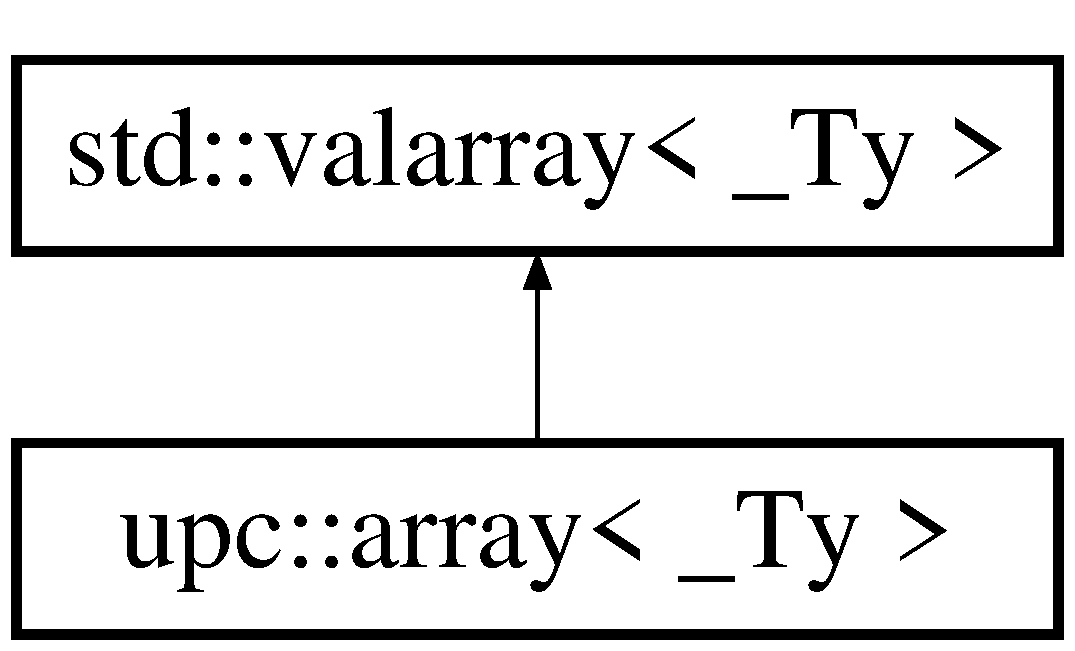
\includegraphics[height=2.000000cm]{classupc_1_1array}
\end{center}
\end{figure}
\subsection*{Public Types}
\begin{DoxyCompactItemize}
\item 
typedef \hyperlink{classupc_1_1array}{array}$<$ \+\_\+\+Ty $>$ \hyperlink{classupc_1_1array_a9c800a9bf971fc1d7c02a34803f87115}{\+\_\+\+Myt}
\item 
typedef uint32\+\_\+t \hyperlink{classupc_1_1array_a85501f086a20ed6686ef78a242b2f302}{size\+\_\+type}
\item 
typedef \+\_\+\+A\+::pointer \hyperlink{classupc_1_1array_a4ef66945898a2c393cff5be41de077d2}{\+\_\+\+Tptr}
\item 
typedef \+\_\+\+A\+::const\+\_\+pointer \hyperlink{classupc_1_1array_a420718228a4d845721303a19755f0d42}{\+\_\+\+Ctptr}
\item 
typedef \+\_\+\+A\+::reference \hyperlink{classupc_1_1array_a99066373537d57ee780ce4d3396314f8}{reference}
\item 
typedef \+\_\+\+A\+::const\+\_\+reference \hyperlink{classupc_1_1array_a3b639eaadbf9a2c410d7c02d3d1c01e4}{const\+\_\+reference}
\end{DoxyCompactItemize}
\subsection*{Public Member Functions}
\begin{DoxyCompactItemize}
\item 
\hyperlink{classupc_1_1array_a91a96a5d4ba2076aa8d221916d8376a2}{array} (unsigned int size=0)
\item 
\hyperlink{classupc_1_1array_a420718228a4d845721303a19755f0d42}{\+\_\+\+Ctptr} \hyperlink{classupc_1_1array_a160dca0372cf7ec405a44e6c43852381}{v} () const 
\item 
\hyperlink{classupc_1_1array_a4ef66945898a2c393cff5be41de077d2}{\+\_\+\+Tptr} \hyperlink{classupc_1_1array_a1b5e50b24d426dd6652139190c0d5b62}{v} ()
\item 
void \hyperlink{classupc_1_1array_aeb72a62336fc9474afdf3fa6f5cea9ca}{reset} ()
\end{DoxyCompactItemize}
\subsection*{Private Types}
\begin{DoxyCompactItemize}
\item 
typedef std\+::valarray$<$ \+\_\+\+Ty $>$ \hyperlink{classupc_1_1array_a2d2187ace46e59d689195d96a53e9965}{Tvalarray}
\item 
typedef std\+::allocator$<$ \+\_\+\+Ty $>$ \hyperlink{classupc_1_1array_a5eeaa143aa0b098c7402952d1f9c7ea7}{\+\_\+A}
\end{DoxyCompactItemize}


\subsection{Member Typedef Documentation}
\index{upc\+::array@{upc\+::array}!\+\_\+A@{\+\_\+A}}
\index{\+\_\+A@{\+\_\+A}!upc\+::array@{upc\+::array}}
\subsubsection[{\texorpdfstring{\+\_\+A}{_A}}]{\setlength{\rightskip}{0pt plus 5cm}template$<$class \+\_\+\+Ty$>$ typedef std\+::allocator$<$\+\_\+\+Ty$>$ {\bf upc\+::array}$<$ \+\_\+\+Ty $>$\+::{\bf \+\_\+A}\hspace{0.3cm}{\ttfamily [private]}}\hypertarget{classupc_1_1array_a5eeaa143aa0b098c7402952d1f9c7ea7}{}\label{classupc_1_1array_a5eeaa143aa0b098c7402952d1f9c7ea7}
\index{upc\+::array@{upc\+::array}!\+\_\+\+Ctptr@{\+\_\+\+Ctptr}}
\index{\+\_\+\+Ctptr@{\+\_\+\+Ctptr}!upc\+::array@{upc\+::array}}
\subsubsection[{\texorpdfstring{\+\_\+\+Ctptr}{_Ctptr}}]{\setlength{\rightskip}{0pt plus 5cm}template$<$class \+\_\+\+Ty$>$ typedef \+\_\+\+A\+::const\+\_\+pointer {\bf upc\+::array}$<$ \+\_\+\+Ty $>$\+::{\bf \+\_\+\+Ctptr}}\hypertarget{classupc_1_1array_a420718228a4d845721303a19755f0d42}{}\label{classupc_1_1array_a420718228a4d845721303a19755f0d42}
\index{upc\+::array@{upc\+::array}!\+\_\+\+Myt@{\+\_\+\+Myt}}
\index{\+\_\+\+Myt@{\+\_\+\+Myt}!upc\+::array@{upc\+::array}}
\subsubsection[{\texorpdfstring{\+\_\+\+Myt}{_Myt}}]{\setlength{\rightskip}{0pt plus 5cm}template$<$class \+\_\+\+Ty$>$ typedef {\bf array}$<$\+\_\+\+Ty$>$ {\bf upc\+::array}$<$ \+\_\+\+Ty $>$\+::{\bf \+\_\+\+Myt}}\hypertarget{classupc_1_1array_a9c800a9bf971fc1d7c02a34803f87115}{}\label{classupc_1_1array_a9c800a9bf971fc1d7c02a34803f87115}
\index{upc\+::array@{upc\+::array}!\+\_\+\+Tptr@{\+\_\+\+Tptr}}
\index{\+\_\+\+Tptr@{\+\_\+\+Tptr}!upc\+::array@{upc\+::array}}
\subsubsection[{\texorpdfstring{\+\_\+\+Tptr}{_Tptr}}]{\setlength{\rightskip}{0pt plus 5cm}template$<$class \+\_\+\+Ty$>$ typedef \+\_\+\+A\+::pointer {\bf upc\+::array}$<$ \+\_\+\+Ty $>$\+::{\bf \+\_\+\+Tptr}}\hypertarget{classupc_1_1array_a4ef66945898a2c393cff5be41de077d2}{}\label{classupc_1_1array_a4ef66945898a2c393cff5be41de077d2}
\index{upc\+::array@{upc\+::array}!const\+\_\+reference@{const\+\_\+reference}}
\index{const\+\_\+reference@{const\+\_\+reference}!upc\+::array@{upc\+::array}}
\subsubsection[{\texorpdfstring{const\+\_\+reference}{const_reference}}]{\setlength{\rightskip}{0pt plus 5cm}template$<$class \+\_\+\+Ty$>$ typedef \+\_\+\+A\+::const\+\_\+reference {\bf upc\+::array}$<$ \+\_\+\+Ty $>$\+::{\bf const\+\_\+reference}}\hypertarget{classupc_1_1array_a3b639eaadbf9a2c410d7c02d3d1c01e4}{}\label{classupc_1_1array_a3b639eaadbf9a2c410d7c02d3d1c01e4}
\index{upc\+::array@{upc\+::array}!reference@{reference}}
\index{reference@{reference}!upc\+::array@{upc\+::array}}
\subsubsection[{\texorpdfstring{reference}{reference}}]{\setlength{\rightskip}{0pt plus 5cm}template$<$class \+\_\+\+Ty$>$ typedef \+\_\+\+A\+::reference {\bf upc\+::array}$<$ \+\_\+\+Ty $>$\+::{\bf reference}}\hypertarget{classupc_1_1array_a99066373537d57ee780ce4d3396314f8}{}\label{classupc_1_1array_a99066373537d57ee780ce4d3396314f8}
\index{upc\+::array@{upc\+::array}!size\+\_\+type@{size\+\_\+type}}
\index{size\+\_\+type@{size\+\_\+type}!upc\+::array@{upc\+::array}}
\subsubsection[{\texorpdfstring{size\+\_\+type}{size_type}}]{\setlength{\rightskip}{0pt plus 5cm}template$<$class \+\_\+\+Ty$>$ typedef uint32\+\_\+t {\bf upc\+::array}$<$ \+\_\+\+Ty $>$\+::{\bf size\+\_\+type}}\hypertarget{classupc_1_1array_a85501f086a20ed6686ef78a242b2f302}{}\label{classupc_1_1array_a85501f086a20ed6686ef78a242b2f302}
\index{upc\+::array@{upc\+::array}!Tvalarray@{Tvalarray}}
\index{Tvalarray@{Tvalarray}!upc\+::array@{upc\+::array}}
\subsubsection[{\texorpdfstring{Tvalarray}{Tvalarray}}]{\setlength{\rightskip}{0pt plus 5cm}template$<$class \+\_\+\+Ty$>$ typedef std\+::valarray$<$\+\_\+\+Ty$>$ {\bf upc\+::array}$<$ \+\_\+\+Ty $>$\+::{\bf Tvalarray}\hspace{0.3cm}{\ttfamily [private]}}\hypertarget{classupc_1_1array_a2d2187ace46e59d689195d96a53e9965}{}\label{classupc_1_1array_a2d2187ace46e59d689195d96a53e9965}


\subsection{Constructor \& Destructor Documentation}
\index{upc\+::array@{upc\+::array}!array@{array}}
\index{array@{array}!upc\+::array@{upc\+::array}}
\subsubsection[{\texorpdfstring{array(unsigned int size=0)}{array(unsigned int size=0)}}]{\setlength{\rightskip}{0pt plus 5cm}template$<$class \+\_\+\+Ty$>$ {\bf upc\+::array}$<$ \+\_\+\+Ty $>$\+::{\bf array} (
\begin{DoxyParamCaption}
\item[{unsigned int}]{size = {\ttfamily 0}}
\end{DoxyParamCaption}
)\hspace{0.3cm}{\ttfamily [inline]}, {\ttfamily [explicit]}}\hypertarget{classupc_1_1array_a91a96a5d4ba2076aa8d221916d8376a2}{}\label{classupc_1_1array_a91a96a5d4ba2076aa8d221916d8376a2}


\subsection{Member Function Documentation}
\index{upc\+::array@{upc\+::array}!reset@{reset}}
\index{reset@{reset}!upc\+::array@{upc\+::array}}
\subsubsection[{\texorpdfstring{reset()}{reset()}}]{\setlength{\rightskip}{0pt plus 5cm}template$<$class \+\_\+\+Ty$>$ void {\bf upc\+::array}$<$ \+\_\+\+Ty $>$\+::reset (
\begin{DoxyParamCaption}
{}
\end{DoxyParamCaption}
)\hspace{0.3cm}{\ttfamily [inline]}}\hypertarget{classupc_1_1array_aeb72a62336fc9474afdf3fa6f5cea9ca}{}\label{classupc_1_1array_aeb72a62336fc9474afdf3fa6f5cea9ca}
\index{upc\+::array@{upc\+::array}!v@{v}}
\index{v@{v}!upc\+::array@{upc\+::array}}
\subsubsection[{\texorpdfstring{v() const }{v() const }}]{\setlength{\rightskip}{0pt plus 5cm}template$<$class \+\_\+\+Ty$>$ {\bf \+\_\+\+Ctptr} {\bf upc\+::array}$<$ \+\_\+\+Ty $>$\+::v (
\begin{DoxyParamCaption}
{}
\end{DoxyParamCaption}
) const\hspace{0.3cm}{\ttfamily [inline]}}\hypertarget{classupc_1_1array_a160dca0372cf7ec405a44e6c43852381}{}\label{classupc_1_1array_a160dca0372cf7ec405a44e6c43852381}
\index{upc\+::array@{upc\+::array}!v@{v}}
\index{v@{v}!upc\+::array@{upc\+::array}}
\subsubsection[{\texorpdfstring{v()}{v()}}]{\setlength{\rightskip}{0pt plus 5cm}template$<$class \+\_\+\+Ty$>$ {\bf \+\_\+\+Tptr} {\bf upc\+::array}$<$ \+\_\+\+Ty $>$\+::v (
\begin{DoxyParamCaption}
{}
\end{DoxyParamCaption}
)\hspace{0.3cm}{\ttfamily [inline]}}\hypertarget{classupc_1_1array_a1b5e50b24d426dd6652139190c0d5b62}{}\label{classupc_1_1array_a1b5e50b24d426dd6652139190c0d5b62}


The documentation for this class was generated from the following file\+:\begin{DoxyCompactItemize}
\item 
include/\hyperlink{matrix_8h}{matrix.\+h}\end{DoxyCompactItemize}

\hypertarget{classupc_1_1CircularIndex}{}\section{upc\+:\+:Circular\+Index Class Reference}
\label{classupc_1_1CircularIndex}\index{upc\+::\+Circular\+Index@{upc\+::\+Circular\+Index}}


Circular Index used to go through state circular buffer (u)  




{\ttfamily \#include $<$digital\+\_\+filter.\+h$>$}

\subsection*{Public Member Functions}
\begin{DoxyCompactItemize}
\item 
\hyperlink{classupc_1_1CircularIndex_a80c03ec94380d80132ca01b39ef9b0e7}{Circular\+Index} (int s=1)
\begin{DoxyCompactList}\small\item\em buffer size; index goes from 0 ... size-\/1 \end{DoxyCompactList}\item 
\hyperlink{classupc_1_1CircularIndex_abca2976e157594a74d4aa1c06b0c4c2e}{Circular\+Index} (\hyperlink{classupc_1_1CircularIndex}{Circular\+Index} \&ci)
\begin{DoxyCompactList}\small\item\em constructor defining size based on other \hyperlink{classupc_1_1CircularIndex}{Circular\+Index} \end{DoxyCompactList}\item 
void \hyperlink{classupc_1_1CircularIndex_aa8bfc28723ab87c1ab66262843aac2a5}{resize} (int s)
\begin{DoxyCompactList}\small\item\em Set size of circular index. \end{DoxyCompactList}\item 
\hyperlink{classupc_1_1CircularIndex}{Circular\+Index} \& \hyperlink{classupc_1_1CircularIndex_a8c02bb1020495ad418f1c0770a03a9f6}{operator++} ()
\begin{DoxyCompactList}\small\item\em Increment. \end{DoxyCompactList}\item 
\hyperlink{classupc_1_1CircularIndex}{Circular\+Index} \& \hyperlink{classupc_1_1CircularIndex_a687ae675e4a3f8a95fc69eb0b961c0a5}{operator+=} (int i)
\begin{DoxyCompactList}\small\item\em Increment \textquotesingle{}i\textquotesingle{} positions. \end{DoxyCompactList}\item 
\hyperlink{classupc_1_1CircularIndex}{Circular\+Index} \& \hyperlink{classupc_1_1CircularIndex_a1e03db5aad51600b2804b7866af81b01}{operator+} (int i)
\begin{DoxyCompactList}\small\item\em Increment \textquotesingle{}i\textquotesingle{} positions. \end{DoxyCompactList}\item 
\hyperlink{classupc_1_1CircularIndex}{Circular\+Index} \& \hyperlink{classupc_1_1CircularIndex_a4527e57789e25c6157111ab491cc38a9}{operator-\/-\/} ()
\begin{DoxyCompactList}\small\item\em Decrement. \end{DoxyCompactList}\item 
\hyperlink{classupc_1_1CircularIndex}{Circular\+Index} \& \hyperlink{classupc_1_1CircularIndex_a4b2892d8a0b891b90bcb34ee55c3d613}{operator-\/=} (int i)
\begin{DoxyCompactList}\small\item\em Decrement \textquotesingle{}i\textquotesingle{} positions. \end{DoxyCompactList}\item 
\hyperlink{classupc_1_1CircularIndex}{Circular\+Index} \& \hyperlink{classupc_1_1CircularIndex_a7745755030622a01389f2133632d7f76}{operator-\/} (int i)
\begin{DoxyCompactList}\small\item\em Decrement \textquotesingle{}i\textquotesingle{} positions. \end{DoxyCompactList}\item 
\hyperlink{classupc_1_1CircularIndex_ab0961d598cc0a51a2990e8823f71a332}{operator int} ()
\item 
\hyperlink{classupc_1_1CircularIndex}{Circular\+Index} \& \hyperlink{classupc_1_1CircularIndex_ab23f2d6ba2b5781153bcf6383cce8afc}{operator=} (const \hyperlink{classupc_1_1CircularIndex}{Circular\+Index} \&ci)
\begin{DoxyCompactList}\small\item\em !\+Casting from \hyperlink{classupc_1_1CircularIndex}{Circular\+Index} to int, returning int. \end{DoxyCompactList}\end{DoxyCompactItemize}
\subsection*{Private Attributes}
\begin{DoxyCompactItemize}
\item 
int \hyperlink{classupc_1_1CircularIndex_a0d0973d1fc7fa4200ac39dc2880e0081}{index}
\item 
int \hyperlink{classupc_1_1CircularIndex_ab53d382eeb825c3583964729c477ffae}{size}
\begin{DoxyCompactList}\small\item\em the index (value) \end{DoxyCompactList}\end{DoxyCompactItemize}


\subsection{Detailed Description}
Circular Index used to go through state circular buffer (u) 

The circular index is a simple class to address a circular buffer. Once the buffer size is defined, you can add or substract and the index remains inside the buffer. A casting operator to int is provided.

Example\+: 
\begin{DoxyCode}
\textcolor{keywordtype}{float} \hyperlink{FFTReal__readme_8txt_a9c92ac89d1560f812393ca39a19e581e}{x}[8]=\{0,1,2,4,5,6,7\};
\hyperlink{classupc_1_1CircularIndex_a80c03ec94380d80132ca01b39ef9b0e7}{CircularIndex} ci(8);
\textcolor{keywordtype}{int} n=10; \textcolor{keywordtype}{float} z=0.0F;
\textcolor{keywordflow}{for} (n=0; n< 10; ++n, ++ci)
    z += x[ci+1] - x[ci-1];
\end{DoxyCode}
 Operations +, +=, ++, -\/, -\/=, -- are defined 

\subsection{Constructor \& Destructor Documentation}
\index{upc\+::\+Circular\+Index@{upc\+::\+Circular\+Index}!Circular\+Index@{Circular\+Index}}
\index{Circular\+Index@{Circular\+Index}!upc\+::\+Circular\+Index@{upc\+::\+Circular\+Index}}
\subsubsection[{\texorpdfstring{Circular\+Index(int s=1)}{CircularIndex(int s=1)}}]{\setlength{\rightskip}{0pt plus 5cm}upc\+::\+Circular\+Index\+::\+Circular\+Index (
\begin{DoxyParamCaption}
\item[{int}]{s = {\ttfamily 1}}
\end{DoxyParamCaption}
)\hspace{0.3cm}{\ttfamily [inline]}}\hypertarget{classupc_1_1CircularIndex_a80c03ec94380d80132ca01b39ef9b0e7}{}\label{classupc_1_1CircularIndex_a80c03ec94380d80132ca01b39ef9b0e7}


buffer size; index goes from 0 ... size-\/1 

default\+: size=1; not very useful (index can only be 0) \index{upc\+::\+Circular\+Index@{upc\+::\+Circular\+Index}!Circular\+Index@{Circular\+Index}}
\index{Circular\+Index@{Circular\+Index}!upc\+::\+Circular\+Index@{upc\+::\+Circular\+Index}}
\subsubsection[{\texorpdfstring{Circular\+Index(\+Circular\+Index \&ci)}{CircularIndex(CircularIndex &ci)}}]{\setlength{\rightskip}{0pt plus 5cm}upc\+::\+Circular\+Index\+::\+Circular\+Index (
\begin{DoxyParamCaption}
\item[{{\bf Circular\+Index} \&}]{ci}
\end{DoxyParamCaption}
)\hspace{0.3cm}{\ttfamily [inline]}}\hypertarget{classupc_1_1CircularIndex_abca2976e157594a74d4aa1c06b0c4c2e}{}\label{classupc_1_1CircularIndex_abca2976e157594a74d4aa1c06b0c4c2e}


constructor defining size based on other \hyperlink{classupc_1_1CircularIndex}{Circular\+Index} 



\subsection{Member Function Documentation}
\index{upc\+::\+Circular\+Index@{upc\+::\+Circular\+Index}!operator int@{operator int}}
\index{operator int@{operator int}!upc\+::\+Circular\+Index@{upc\+::\+Circular\+Index}}
\subsubsection[{\texorpdfstring{operator int()}{operator int()}}]{\setlength{\rightskip}{0pt plus 5cm}upc\+::\+Circular\+Index\+::operator int (
\begin{DoxyParamCaption}
{}
\end{DoxyParamCaption}
)\hspace{0.3cm}{\ttfamily [inline]}}\hypertarget{classupc_1_1CircularIndex_ab0961d598cc0a51a2990e8823f71a332}{}\label{classupc_1_1CircularIndex_ab0961d598cc0a51a2990e8823f71a332}
\index{upc\+::\+Circular\+Index@{upc\+::\+Circular\+Index}!operator+@{operator+}}
\index{operator+@{operator+}!upc\+::\+Circular\+Index@{upc\+::\+Circular\+Index}}
\subsubsection[{\texorpdfstring{operator+(int i)}{operator+(int i)}}]{\setlength{\rightskip}{0pt plus 5cm}{\bf Circular\+Index}\& upc\+::\+Circular\+Index\+::operator+ (
\begin{DoxyParamCaption}
\item[{int}]{i}
\end{DoxyParamCaption}
)\hspace{0.3cm}{\ttfamily [inline]}}\hypertarget{classupc_1_1CircularIndex_a1e03db5aad51600b2804b7866af81b01}{}\label{classupc_1_1CircularIndex_a1e03db5aad51600b2804b7866af81b01}


Increment \textquotesingle{}i\textquotesingle{} positions. 

\index{upc\+::\+Circular\+Index@{upc\+::\+Circular\+Index}!operator++@{operator++}}
\index{operator++@{operator++}!upc\+::\+Circular\+Index@{upc\+::\+Circular\+Index}}
\subsubsection[{\texorpdfstring{operator++()}{operator++()}}]{\setlength{\rightskip}{0pt plus 5cm}{\bf Circular\+Index}\& upc\+::\+Circular\+Index\+::operator++ (
\begin{DoxyParamCaption}
{}
\end{DoxyParamCaption}
)\hspace{0.3cm}{\ttfamily [inline]}}\hypertarget{classupc_1_1CircularIndex_a8c02bb1020495ad418f1c0770a03a9f6}{}\label{classupc_1_1CircularIndex_a8c02bb1020495ad418f1c0770a03a9f6}


Increment. 

\index{upc\+::\+Circular\+Index@{upc\+::\+Circular\+Index}!operator+=@{operator+=}}
\index{operator+=@{operator+=}!upc\+::\+Circular\+Index@{upc\+::\+Circular\+Index}}
\subsubsection[{\texorpdfstring{operator+=(int i)}{operator+=(int i)}}]{\setlength{\rightskip}{0pt plus 5cm}{\bf Circular\+Index}\& upc\+::\+Circular\+Index\+::operator+= (
\begin{DoxyParamCaption}
\item[{int}]{i}
\end{DoxyParamCaption}
)\hspace{0.3cm}{\ttfamily [inline]}}\hypertarget{classupc_1_1CircularIndex_a687ae675e4a3f8a95fc69eb0b961c0a5}{}\label{classupc_1_1CircularIndex_a687ae675e4a3f8a95fc69eb0b961c0a5}


Increment \textquotesingle{}i\textquotesingle{} positions. 

\index{upc\+::\+Circular\+Index@{upc\+::\+Circular\+Index}!operator-\/@{operator-\/}}
\index{operator-\/@{operator-\/}!upc\+::\+Circular\+Index@{upc\+::\+Circular\+Index}}
\subsubsection[{\texorpdfstring{operator-\/(int i)}{operator-(int i)}}]{\setlength{\rightskip}{0pt plus 5cm}{\bf Circular\+Index}\& upc\+::\+Circular\+Index\+::operator-\/ (
\begin{DoxyParamCaption}
\item[{int}]{i}
\end{DoxyParamCaption}
)\hspace{0.3cm}{\ttfamily [inline]}}\hypertarget{classupc_1_1CircularIndex_a7745755030622a01389f2133632d7f76}{}\label{classupc_1_1CircularIndex_a7745755030622a01389f2133632d7f76}


Decrement \textquotesingle{}i\textquotesingle{} positions. 

\index{upc\+::\+Circular\+Index@{upc\+::\+Circular\+Index}!operator-\/-\/@{operator-\/-\/}}
\index{operator-\/-\/@{operator-\/-\/}!upc\+::\+Circular\+Index@{upc\+::\+Circular\+Index}}
\subsubsection[{\texorpdfstring{operator-\/-\/()}{operator--()}}]{\setlength{\rightskip}{0pt plus 5cm}{\bf Circular\+Index}\& upc\+::\+Circular\+Index\+::operator-\/-\/ (
\begin{DoxyParamCaption}
{}
\end{DoxyParamCaption}
)\hspace{0.3cm}{\ttfamily [inline]}}\hypertarget{classupc_1_1CircularIndex_a4527e57789e25c6157111ab491cc38a9}{}\label{classupc_1_1CircularIndex_a4527e57789e25c6157111ab491cc38a9}


Decrement. 

\index{upc\+::\+Circular\+Index@{upc\+::\+Circular\+Index}!operator-\/=@{operator-\/=}}
\index{operator-\/=@{operator-\/=}!upc\+::\+Circular\+Index@{upc\+::\+Circular\+Index}}
\subsubsection[{\texorpdfstring{operator-\/=(int i)}{operator-=(int i)}}]{\setlength{\rightskip}{0pt plus 5cm}{\bf Circular\+Index}\& upc\+::\+Circular\+Index\+::operator-\/= (
\begin{DoxyParamCaption}
\item[{int}]{i}
\end{DoxyParamCaption}
)\hspace{0.3cm}{\ttfamily [inline]}}\hypertarget{classupc_1_1CircularIndex_a4b2892d8a0b891b90bcb34ee55c3d613}{}\label{classupc_1_1CircularIndex_a4b2892d8a0b891b90bcb34ee55c3d613}


Decrement \textquotesingle{}i\textquotesingle{} positions. 

\index{upc\+::\+Circular\+Index@{upc\+::\+Circular\+Index}!operator=@{operator=}}
\index{operator=@{operator=}!upc\+::\+Circular\+Index@{upc\+::\+Circular\+Index}}
\subsubsection[{\texorpdfstring{operator=(const Circular\+Index \&ci)}{operator=(const CircularIndex &ci)}}]{\setlength{\rightskip}{0pt plus 5cm}{\bf Circular\+Index}\& upc\+::\+Circular\+Index\+::operator= (
\begin{DoxyParamCaption}
\item[{const {\bf Circular\+Index} \&}]{ci}
\end{DoxyParamCaption}
)\hspace{0.3cm}{\ttfamily [inline]}}\hypertarget{classupc_1_1CircularIndex_ab23f2d6ba2b5781153bcf6383cce8afc}{}\label{classupc_1_1CircularIndex_ab23f2d6ba2b5781153bcf6383cce8afc}


!\+Casting from \hyperlink{classupc_1_1CircularIndex}{Circular\+Index} to int, returning int. 

\index{upc\+::\+Circular\+Index@{upc\+::\+Circular\+Index}!resize@{resize}}
\index{resize@{resize}!upc\+::\+Circular\+Index@{upc\+::\+Circular\+Index}}
\subsubsection[{\texorpdfstring{resize(int s)}{resize(int s)}}]{\setlength{\rightskip}{0pt plus 5cm}void upc\+::\+Circular\+Index\+::resize (
\begin{DoxyParamCaption}
\item[{int}]{s}
\end{DoxyParamCaption}
)\hspace{0.3cm}{\ttfamily [inline]}}\hypertarget{classupc_1_1CircularIndex_aa8bfc28723ab87c1ab66262843aac2a5}{}\label{classupc_1_1CircularIndex_aa8bfc28723ab87c1ab66262843aac2a5}


Set size of circular index. 



\subsection{Member Data Documentation}
\index{upc\+::\+Circular\+Index@{upc\+::\+Circular\+Index}!index@{index}}
\index{index@{index}!upc\+::\+Circular\+Index@{upc\+::\+Circular\+Index}}
\subsubsection[{\texorpdfstring{index}{index}}]{\setlength{\rightskip}{0pt plus 5cm}int upc\+::\+Circular\+Index\+::index\hspace{0.3cm}{\ttfamily [private]}}\hypertarget{classupc_1_1CircularIndex_a0d0973d1fc7fa4200ac39dc2880e0081}{}\label{classupc_1_1CircularIndex_a0d0973d1fc7fa4200ac39dc2880e0081}
\index{upc\+::\+Circular\+Index@{upc\+::\+Circular\+Index}!size@{size}}
\index{size@{size}!upc\+::\+Circular\+Index@{upc\+::\+Circular\+Index}}
\subsubsection[{\texorpdfstring{size}{size}}]{\setlength{\rightskip}{0pt plus 5cm}int upc\+::\+Circular\+Index\+::size\hspace{0.3cm}{\ttfamily [private]}}\hypertarget{classupc_1_1CircularIndex_ab53d382eeb825c3583964729c477ffae}{}\label{classupc_1_1CircularIndex_ab53d382eeb825c3583964729c477ffae}


the index (value) 



The documentation for this class was generated from the following file\+:\begin{DoxyCompactItemize}
\item 
include/\hyperlink{digital__filter_8h}{digital\+\_\+filter.\+h}\end{DoxyCompactItemize}

\hypertarget{classupc_1_1DigitalFilter}{}\section{upc\+:\+:Digital\+Filter Class Reference}
\label{classupc_1_1DigitalFilter}\index{upc\+::\+Digital\+Filter@{upc\+::\+Digital\+Filter}}


Digital filter implemented using direct form.  




{\ttfamily \#include $<$digital\+\_\+filter.\+h$>$}

\subsection*{Public Member Functions}
\begin{DoxyCompactItemize}
\item 
\hyperlink{classupc_1_1DigitalFilter_a3d8e61b92170380d06b26aee1ebc1f16}{Digital\+Filter} (const std\+::vector$<$ \hyperlink{FFTReal__readme_8txt_a0ea2fae2a8106200bf378b90eae003cf}{float} $>$ \&\+\_\+a, const std\+::vector$<$ \hyperlink{FFTReal__readme_8txt_a0ea2fae2a8106200bf378b90eae003cf}{float} $>$ \&\+\_\+b, \hyperlink{FFTReal__readme_8txt_a0ea2fae2a8106200bf378b90eae003cf}{float} g=1.\+0\+F)
\begin{DoxyCompactList}\small\item\em Create filter. \end{DoxyCompactList}\item 
\hyperlink{classupc_1_1DigitalFilter_ac3c32e0d51a88354482f13528e9a7842}{Digital\+Filter} ()
\begin{DoxyCompactList}\small\item\em create void filter H(z) = 1 \end{DoxyCompactList}\item 
void \hyperlink{classupc_1_1DigitalFilter_ade3c3a24bbfbc1b2edbf4bcd0885a9e6}{set\+\_\+a} (std\+::vector$<$ \hyperlink{FFTReal__readme_8txt_a0ea2fae2a8106200bf378b90eae003cf}{float} $>$ const \&A)
\begin{DoxyCompactList}\small\item\em Change denominator (state conditions only cleaned if order changes) \end{DoxyCompactList}\item 
void \hyperlink{classupc_1_1DigitalFilter_a9f23a5e9db027eb0c9b70bd9b5d08e09}{set\+\_\+b} (const std\+::vector$<$ \hyperlink{FFTReal__readme_8txt_a0ea2fae2a8106200bf378b90eae003cf}{float} $>$ \&B)
\begin{DoxyCompactList}\small\item\em Change denominator (state conditions only cleaned if order changes) \end{DoxyCompactList}\item 
\hyperlink{classupc_1_1DigitalFilter_a54937beb73f0789cb9265498522da628}{Digital\+Filter} (const \hyperlink{classupc_1_1DigitalFilter}{Digital\+Filter} \&\hyperlink{FFTReal__readme_8txt_abbf3cc73d1e3e4714ab1639819396eca}{f})
\item 
\hyperlink{classupc_1_1DigitalFilter}{Digital\+Filter} \& \hyperlink{classupc_1_1DigitalFilter_a26527559b1b71aad240deca22f5599ec}{operator=} (const \hyperlink{classupc_1_1DigitalFilter}{Digital\+Filter} \&\hyperlink{FFTReal__readme_8txt_abbf3cc73d1e3e4714ab1639819396eca}{f})
\begin{DoxyCompactList}\small\item\em Asign operator (copy a filter from other) \end{DoxyCompactList}\item 
void \hyperlink{classupc_1_1DigitalFilter_a2b97aaeacac8b5a8b52e1bd8fc295970}{set\+\_\+resonator} (\hyperlink{FFTReal__readme_8txt_a0ea2fae2a8106200bf378b90eae003cf}{float} norm\+\_\+central\+\_\+freq, \hyperlink{FFTReal__readme_8txt_a0ea2fae2a8106200bf378b90eae003cf}{float} norm\+\_\+bandwidth)
\begin{DoxyCompactList}\small\item\em Second order AR band-\/pass filter defined by central frequency and bandwidth. \end{DoxyCompactList}\item 
void \hyperlink{classupc_1_1DigitalFilter_a506905346c44ac46c292ea1fa1212c3e}{set\+\_\+gain} (\hyperlink{FFTReal__readme_8txt_a0ea2fae2a8106200bf378b90eae003cf}{float} g)
\item 
void \hyperlink{classupc_1_1DigitalFilter_ad6c0f9584687642434081448f85d89f9}{clear} ()
\begin{DoxyCompactList}\small\item\em clean state conditions \end{DoxyCompactList}\item 
\hyperlink{FFTReal__readme_8txt_a0ea2fae2a8106200bf378b90eae003cf}{float} \hyperlink{classupc_1_1DigitalFilter_a8d8f578b514a2dd58a545a68fdf441ee}{operator()} (\hyperlink{FFTReal__readme_8txt_a0ea2fae2a8106200bf378b90eae003cf}{float} \hyperlink{FFTReal__readme_8txt_a9c92ac89d1560f812393ca39a19e581e}{x})
\begin{DoxyCompactList}\small\item\em Filter one sample. \end{DoxyCompactList}\item 
std\+::vector$<$ \hyperlink{FFTReal__readme_8txt_a0ea2fae2a8106200bf378b90eae003cf}{float} $>$ \hyperlink{classupc_1_1DigitalFilter_aea8cdd6504cf9c4ae1a6d9a28e1bcaa4}{operator()} (const std\+::vector$<$ \hyperlink{FFTReal__readme_8txt_a0ea2fae2a8106200bf378b90eae003cf}{float} $>$ \&\hyperlink{FFTReal__readme_8txt_a9c92ac89d1560f812393ca39a19e581e}{x})
\begin{DoxyCompactList}\small\item\em Filter a vector of samples. \end{DoxyCompactList}\item 
void \hyperlink{classupc_1_1DigitalFilter_a08b53e2a3884053f4a48d6860194cccb}{operator()} (std\+::vector$<$ \hyperlink{FFTReal__readme_8txt_a0ea2fae2a8106200bf378b90eae003cf}{float} $>$\+::const\+\_\+iterator beg\+Src, std\+::vector$<$ \hyperlink{FFTReal__readme_8txt_a0ea2fae2a8106200bf378b90eae003cf}{float} $>$\+::const\+\_\+iterator end\+Src, std\+::vector$<$ \hyperlink{FFTReal__readme_8txt_a0ea2fae2a8106200bf378b90eae003cf}{float} $>$\+::iterator beg\+Dst)
\begin{DoxyCompactList}\small\item\em Filter several samples, from beg\+Src to end\+Src, and save at beg\+Dst and following positions. \end{DoxyCompactList}\item 
std\+::vector$<$ \hyperlink{FFTReal__readme_8txt_a0ea2fae2a8106200bf378b90eae003cf}{float} $>$ \hyperlink{classupc_1_1DigitalFilter_a81e5fab2bf8cbab0e70622b7fa2cfe91}{freqz} (std\+::vector$<$ \hyperlink{FFTReal__readme_8txt_a0ea2fae2a8106200bf378b90eae003cf}{float} $>$ const freq, bool db=true) const 
\item 
std\+::vector$<$ \hyperlink{FFTReal__readme_8txt_a0ea2fae2a8106200bf378b90eae003cf}{float} $>$ \hyperlink{classupc_1_1DigitalFilter_a580b4f2584d0b993e1fc6f9d9256b9f8}{freqz} (unsigned int \hyperlink{FFTReal__readme_8txt_a049dd452c22185832440207517cffdaa}{N}, bool db=true) const 
\item 
\hyperlink{FFTReal__readme_8txt_a0ea2fae2a8106200bf378b90eae003cf}{float} \hyperlink{classupc_1_1DigitalFilter_a9589b9615fbd51754afb757c5431b1e0}{sfreqz} (\hyperlink{FFTReal__readme_8txt_a0ea2fae2a8106200bf378b90eae003cf}{float} freq, bool db=true) const 
\end{DoxyCompactItemize}
\subsection*{Private Member Functions}
\begin{DoxyCompactItemize}
\item 
void \hyperlink{classupc_1_1DigitalFilter_a66ebd4fb1a26af461c4845efbc528236}{prepare\+\_\+state} ()
\begin{DoxyCompactList}\small\item\em Allocate memory for stated conditions. \end{DoxyCompactList}\end{DoxyCompactItemize}
\subsection*{Private Attributes}
\begin{DoxyCompactItemize}
\item 
std\+::vector$<$ \hyperlink{FFTReal__readme_8txt_a0ea2fae2a8106200bf378b90eae003cf}{float} $>$ \hyperlink{classupc_1_1DigitalFilter_a2452cdde3d6845b838d9ebed8099dc4e}{a}
\begin{DoxyCompactList}\small\item\em Denominator A(z) = a0+a1 z$^\wedge$-\/1 + a2 z$^\wedge$-\/2 ... an z$^\wedge$-\/n) \end{DoxyCompactList}\item 
std\+::vector$<$ \hyperlink{FFTReal__readme_8txt_a0ea2fae2a8106200bf378b90eae003cf}{float} $>$ \hyperlink{classupc_1_1DigitalFilter_ad72194d793b429b0f0eea9fab017da68}{b}
\begin{DoxyCompactList}\small\item\em Numerator B(z) = b0+b1 z$^\wedge$-\/1 + b2 z$^\wedge$-\/2 ... bm z$^\wedge$-\/m) \end{DoxyCompactList}\item 
std\+::vector$<$ \hyperlink{FFTReal__readme_8txt_a0ea2fae2a8106200bf378b90eae003cf}{float} $>$ \hyperlink{classupc_1_1DigitalFilter_ad8b8d1c7bde2fca050aa297b66d69179}{u}
\begin{DoxyCompactList}\small\item\em State conditions, implemented as circular buffer; call \char`\"{}clear()\char`\"{} to reset them. \end{DoxyCompactList}\item 
\hyperlink{FFTReal__readme_8txt_a0ea2fae2a8106200bf378b90eae003cf}{float} \hyperlink{classupc_1_1DigitalFilter_aaa94a0d08f87c98612d9471719bd773a}{gain}
\item 
\hyperlink{classupc_1_1CircularIndex}{Circular\+Index} \hyperlink{classupc_1_1DigitalFilter_ae2b58018045cfca38cad387dd4b82e83}{index}
\begin{DoxyCompactList}\small\item\em additional gain factor \end{DoxyCompactList}\end{DoxyCompactItemize}


\subsection{Detailed Description}
Digital filter implemented using direct form. 

This class implements digital filtering. The filter is stored as rational funcion H(z) = g B(z)/A(z) Being g\+: gain B(z) = b0 +b1 z$^\wedge$-\/1 + b2 z$^\wedge$-\/2 ... bm z$^\wedge$-\/m A(z) = a0 +a1 z$^\wedge$-\/1 + a2 z$^\wedge$-\/2 ... an z$^\wedge$-\/n

The state conditions are saved after each call to the filter. The filter is implemented using the direct form. Y(z) = B(z)/A(z) X(z) =$>$ U(z) = X(z)/A(z); Y(z) = B(z) U(z) State conditions\+: u\mbox{[}n\mbox{]}

The state conditions are only cleared either\+:
\begin{DoxyItemize}
\item explicitely calling clean()
\item by a change in filter coeficients that imply an order filter
\end{DoxyItemize}

The filters coefficients are set using \hyperlink{classupc_1_1DigitalFilter_ade3c3a24bbfbc1b2edbf4bcd0885a9e6}{set\+\_\+a()}, \hyperlink{classupc_1_1DigitalFilter_a9f23a5e9db027eb0c9b70bd9b5d08e09}{set\+\_\+b()}, \hyperlink{classupc_1_1DigitalFilter_a506905346c44ac46c292ea1fa1212c3e}{set\+\_\+gain()}. An alternative convinient method exist for 2nd order resonators, using the central frequency and the resonator bandwidth\+: \hyperlink{classupc_1_1DigitalFilter_a2b97aaeacac8b5a8b52e1bd8fc295970}{set\+\_\+resonator()} 

\subsection{Constructor \& Destructor Documentation}
\index{upc\+::\+Digital\+Filter@{upc\+::\+Digital\+Filter}!Digital\+Filter@{Digital\+Filter}}
\index{Digital\+Filter@{Digital\+Filter}!upc\+::\+Digital\+Filter@{upc\+::\+Digital\+Filter}}
\subsubsection[{\texorpdfstring{Digital\+Filter(const std\+::vector$<$ float $>$ \&\+\_\+a, const std\+::vector$<$ float $>$ \&\+\_\+b, float g=1.\+0\+F)}{DigitalFilter(const std::vector< float > &_a, const std::vector< float > &_b, float g=1.0F)}}]{\setlength{\rightskip}{0pt plus 5cm}upc\+::\+Digital\+Filter\+::\+Digital\+Filter (
\begin{DoxyParamCaption}
\item[{const std\+::vector$<$ {\bf float} $>$ \&}]{\+\_\+a, }
\item[{const std\+::vector$<$ {\bf float} $>$ \&}]{\+\_\+b, }
\item[{{\bf float}}]{g = {\ttfamily 1.0F}}
\end{DoxyParamCaption}
)\hspace{0.3cm}{\ttfamily [inline]}}\hypertarget{classupc_1_1DigitalFilter_a3d8e61b92170380d06b26aee1ebc1f16}{}\label{classupc_1_1DigitalFilter_a3d8e61b92170380d06b26aee1ebc1f16}


Create filter. 

\index{upc\+::\+Digital\+Filter@{upc\+::\+Digital\+Filter}!Digital\+Filter@{Digital\+Filter}}
\index{Digital\+Filter@{Digital\+Filter}!upc\+::\+Digital\+Filter@{upc\+::\+Digital\+Filter}}
\subsubsection[{\texorpdfstring{Digital\+Filter()}{DigitalFilter()}}]{\setlength{\rightskip}{0pt plus 5cm}upc\+::\+Digital\+Filter\+::\+Digital\+Filter (
\begin{DoxyParamCaption}
{}
\end{DoxyParamCaption}
)\hspace{0.3cm}{\ttfamily [inline]}}\hypertarget{classupc_1_1DigitalFilter_ac3c32e0d51a88354482f13528e9a7842}{}\label{classupc_1_1DigitalFilter_ac3c32e0d51a88354482f13528e9a7842}


create void filter H(z) = 1 

\index{upc\+::\+Digital\+Filter@{upc\+::\+Digital\+Filter}!Digital\+Filter@{Digital\+Filter}}
\index{Digital\+Filter@{Digital\+Filter}!upc\+::\+Digital\+Filter@{upc\+::\+Digital\+Filter}}
\subsubsection[{\texorpdfstring{Digital\+Filter(const Digital\+Filter \&f)}{DigitalFilter(const DigitalFilter &f)}}]{\setlength{\rightskip}{0pt plus 5cm}upc\+::\+Digital\+Filter\+::\+Digital\+Filter (
\begin{DoxyParamCaption}
\item[{const {\bf Digital\+Filter} \&}]{f}
\end{DoxyParamCaption}
)\hspace{0.3cm}{\ttfamily [inline]}}\hypertarget{classupc_1_1DigitalFilter_a54937beb73f0789cb9265498522da628}{}\label{classupc_1_1DigitalFilter_a54937beb73f0789cb9265498522da628}
Create filter 

\subsection{Member Function Documentation}
\index{upc\+::\+Digital\+Filter@{upc\+::\+Digital\+Filter}!clear@{clear}}
\index{clear@{clear}!upc\+::\+Digital\+Filter@{upc\+::\+Digital\+Filter}}
\subsubsection[{\texorpdfstring{clear()}{clear()}}]{\setlength{\rightskip}{0pt plus 5cm}void upc\+::\+Digital\+Filter\+::clear (
\begin{DoxyParamCaption}
{}
\end{DoxyParamCaption}
)\hspace{0.3cm}{\ttfamily [inline]}}\hypertarget{classupc_1_1DigitalFilter_ad6c0f9584687642434081448f85d89f9}{}\label{classupc_1_1DigitalFilter_ad6c0f9584687642434081448f85d89f9}


clean state conditions 

\index{upc\+::\+Digital\+Filter@{upc\+::\+Digital\+Filter}!freqz@{freqz}}
\index{freqz@{freqz}!upc\+::\+Digital\+Filter@{upc\+::\+Digital\+Filter}}
\subsubsection[{\texorpdfstring{freqz(std\+::vector$<$ float $>$ const freq, bool db=true) const }{freqz(std::vector< float > const freq, bool db=true) const }}]{\setlength{\rightskip}{0pt plus 5cm}std\+::vector$<$ {\bf float} $>$ upc\+::\+Digital\+Filter\+::freqz (
\begin{DoxyParamCaption}
\item[{std\+::vector$<$ {\bf float} $>$ const}]{freq, }
\item[{bool}]{db = {\ttfamily true}}
\end{DoxyParamCaption}
) const}\hypertarget{classupc_1_1DigitalFilter_a81e5fab2bf8cbab0e70622b7fa2cfe91}{}\label{classupc_1_1DigitalFilter_a81e5fab2bf8cbab0e70622b7fa2cfe91}
Get freq. response of filter in the given frequencies (freq). \hyperlink{classupc_1_1DigitalFilter_a9589b9615fbd51754afb757c5431b1e0}{sfreqz()} is called for each given frequency \index{upc\+::\+Digital\+Filter@{upc\+::\+Digital\+Filter}!freqz@{freqz}}
\index{freqz@{freqz}!upc\+::\+Digital\+Filter@{upc\+::\+Digital\+Filter}}
\subsubsection[{\texorpdfstring{freqz(unsigned int N, bool db=true) const }{freqz(unsigned int N, bool db=true) const }}]{\setlength{\rightskip}{0pt plus 5cm}std\+::vector$<$ {\bf float} $>$ upc\+::\+Digital\+Filter\+::freqz (
\begin{DoxyParamCaption}
\item[{unsigned int}]{N, }
\item[{bool}]{db = {\ttfamily true}}
\end{DoxyParamCaption}
) const}\hypertarget{classupc_1_1DigitalFilter_a580b4f2584d0b993e1fc6f9d9256b9f8}{}\label{classupc_1_1DigitalFilter_a580b4f2584d0b993e1fc6f9d9256b9f8}
Get freq. response of filter in N discrite frequencies, from 0 to 0.\+5. \hyperlink{classupc_1_1DigitalFilter_a9589b9615fbd51754afb757c5431b1e0}{sfreqz()} is called for each given frequency \index{upc\+::\+Digital\+Filter@{upc\+::\+Digital\+Filter}!operator()@{operator()}}
\index{operator()@{operator()}!upc\+::\+Digital\+Filter@{upc\+::\+Digital\+Filter}}
\subsubsection[{\texorpdfstring{operator()(float x)}{operator()(float x)}}]{\setlength{\rightskip}{0pt plus 5cm}{\bf float} upc\+::\+Digital\+Filter\+::operator() (
\begin{DoxyParamCaption}
\item[{{\bf float}}]{x}
\end{DoxyParamCaption}
)}\hypertarget{classupc_1_1DigitalFilter_a8d8f578b514a2dd58a545a68fdf441ee}{}\label{classupc_1_1DigitalFilter_a8d8f578b514a2dd58a545a68fdf441ee}


Filter one sample. 

\index{upc\+::\+Digital\+Filter@{upc\+::\+Digital\+Filter}!operator()@{operator()}}
\index{operator()@{operator()}!upc\+::\+Digital\+Filter@{upc\+::\+Digital\+Filter}}
\subsubsection[{\texorpdfstring{operator()(const std\+::vector$<$ float $>$ \&x)}{operator()(const std::vector< float > &x)}}]{\setlength{\rightskip}{0pt plus 5cm}std\+::vector$<$ {\bf float} $>$ upc\+::\+Digital\+Filter\+::operator() (
\begin{DoxyParamCaption}
\item[{const std\+::vector$<$ {\bf float} $>$ \&}]{x}
\end{DoxyParamCaption}
)}\hypertarget{classupc_1_1DigitalFilter_aea8cdd6504cf9c4ae1a6d9a28e1bcaa4}{}\label{classupc_1_1DigitalFilter_aea8cdd6504cf9c4ae1a6d9a28e1bcaa4}


Filter a vector of samples. 

\index{upc\+::\+Digital\+Filter@{upc\+::\+Digital\+Filter}!operator()@{operator()}}
\index{operator()@{operator()}!upc\+::\+Digital\+Filter@{upc\+::\+Digital\+Filter}}
\subsubsection[{\texorpdfstring{operator()(std\+::vector$<$ float $>$\+::const\+\_\+iterator beg\+Src, std\+::vector$<$ float $>$\+::const\+\_\+iterator end\+Src, std\+::vector$<$ float $>$\+::iterator beg\+Dst)}{operator()(std::vector< float >::const_iterator begSrc, std::vector< float >::const_iterator endSrc, std::vector< float >::iterator begDst)}}]{\setlength{\rightskip}{0pt plus 5cm}void upc\+::\+Digital\+Filter\+::operator() (
\begin{DoxyParamCaption}
\item[{std\+::vector$<$ {\bf float} $>$\+::const\+\_\+iterator}]{beg\+Src, }
\item[{std\+::vector$<$ {\bf float} $>$\+::const\+\_\+iterator}]{end\+Src, }
\item[{std\+::vector$<$ {\bf float} $>$\+::iterator}]{beg\+Dst}
\end{DoxyParamCaption}
)}\hypertarget{classupc_1_1DigitalFilter_a08b53e2a3884053f4a48d6860194cccb}{}\label{classupc_1_1DigitalFilter_a08b53e2a3884053f4a48d6860194cccb}


Filter several samples, from beg\+Src to end\+Src, and save at beg\+Dst and following positions. 

\index{upc\+::\+Digital\+Filter@{upc\+::\+Digital\+Filter}!operator=@{operator=}}
\index{operator=@{operator=}!upc\+::\+Digital\+Filter@{upc\+::\+Digital\+Filter}}
\subsubsection[{\texorpdfstring{operator=(const Digital\+Filter \&f)}{operator=(const DigitalFilter &f)}}]{\setlength{\rightskip}{0pt plus 5cm}{\bf Digital\+Filter}\& upc\+::\+Digital\+Filter\+::operator= (
\begin{DoxyParamCaption}
\item[{const {\bf Digital\+Filter} \&}]{f}
\end{DoxyParamCaption}
)\hspace{0.3cm}{\ttfamily [inline]}}\hypertarget{classupc_1_1DigitalFilter_a26527559b1b71aad240deca22f5599ec}{}\label{classupc_1_1DigitalFilter_a26527559b1b71aad240deca22f5599ec}


Asign operator (copy a filter from other) 

\index{upc\+::\+Digital\+Filter@{upc\+::\+Digital\+Filter}!prepare\+\_\+state@{prepare\+\_\+state}}
\index{prepare\+\_\+state@{prepare\+\_\+state}!upc\+::\+Digital\+Filter@{upc\+::\+Digital\+Filter}}
\subsubsection[{\texorpdfstring{prepare\+\_\+state()}{prepare_state()}}]{\setlength{\rightskip}{0pt plus 5cm}void upc\+::\+Digital\+Filter\+::prepare\+\_\+state (
\begin{DoxyParamCaption}
{}
\end{DoxyParamCaption}
)\hspace{0.3cm}{\ttfamily [private]}}\hypertarget{classupc_1_1DigitalFilter_a66ebd4fb1a26af461c4845efbc528236}{}\label{classupc_1_1DigitalFilter_a66ebd4fb1a26af461c4845efbc528236}


Allocate memory for stated conditions. 

Allocate memory for state conditions. \index{upc\+::\+Digital\+Filter@{upc\+::\+Digital\+Filter}!set\+\_\+a@{set\+\_\+a}}
\index{set\+\_\+a@{set\+\_\+a}!upc\+::\+Digital\+Filter@{upc\+::\+Digital\+Filter}}
\subsubsection[{\texorpdfstring{set\+\_\+a(std\+::vector$<$ float $>$ const \&\+A)}{set_a(std::vector< float > const &A)}}]{\setlength{\rightskip}{0pt plus 5cm}void upc\+::\+Digital\+Filter\+::set\+\_\+a (
\begin{DoxyParamCaption}
\item[{std\+::vector$<$ {\bf float} $>$ const \&}]{A}
\end{DoxyParamCaption}
)\hspace{0.3cm}{\ttfamily [inline]}}\hypertarget{classupc_1_1DigitalFilter_ade3c3a24bbfbc1b2edbf4bcd0885a9e6}{}\label{classupc_1_1DigitalFilter_ade3c3a24bbfbc1b2edbf4bcd0885a9e6}


Change denominator (state conditions only cleaned if order changes) 

\index{upc\+::\+Digital\+Filter@{upc\+::\+Digital\+Filter}!set\+\_\+b@{set\+\_\+b}}
\index{set\+\_\+b@{set\+\_\+b}!upc\+::\+Digital\+Filter@{upc\+::\+Digital\+Filter}}
\subsubsection[{\texorpdfstring{set\+\_\+b(const std\+::vector$<$ float $>$ \&\+B)}{set_b(const std::vector< float > &B)}}]{\setlength{\rightskip}{0pt plus 5cm}void upc\+::\+Digital\+Filter\+::set\+\_\+b (
\begin{DoxyParamCaption}
\item[{const std\+::vector$<$ {\bf float} $>$ \&}]{B}
\end{DoxyParamCaption}
)\hspace{0.3cm}{\ttfamily [inline]}}\hypertarget{classupc_1_1DigitalFilter_a9f23a5e9db027eb0c9b70bd9b5d08e09}{}\label{classupc_1_1DigitalFilter_a9f23a5e9db027eb0c9b70bd9b5d08e09}


Change denominator (state conditions only cleaned if order changes) 

\index{upc\+::\+Digital\+Filter@{upc\+::\+Digital\+Filter}!set\+\_\+gain@{set\+\_\+gain}}
\index{set\+\_\+gain@{set\+\_\+gain}!upc\+::\+Digital\+Filter@{upc\+::\+Digital\+Filter}}
\subsubsection[{\texorpdfstring{set\+\_\+gain(float g)}{set_gain(float g)}}]{\setlength{\rightskip}{0pt plus 5cm}void upc\+::\+Digital\+Filter\+::set\+\_\+gain (
\begin{DoxyParamCaption}
\item[{{\bf float}}]{g}
\end{DoxyParamCaption}
)\hspace{0.3cm}{\ttfamily [inline]}}\hypertarget{classupc_1_1DigitalFilter_a506905346c44ac46c292ea1fa1212c3e}{}\label{classupc_1_1DigitalFilter_a506905346c44ac46c292ea1fa1212c3e}
\index{upc\+::\+Digital\+Filter@{upc\+::\+Digital\+Filter}!set\+\_\+resonator@{set\+\_\+resonator}}
\index{set\+\_\+resonator@{set\+\_\+resonator}!upc\+::\+Digital\+Filter@{upc\+::\+Digital\+Filter}}
\subsubsection[{\texorpdfstring{set\+\_\+resonator(float norm\+\_\+central\+\_\+freq, float norm\+\_\+bandwidth)}{set_resonator(float norm_central_freq, float norm_bandwidth)}}]{\setlength{\rightskip}{0pt plus 5cm}void upc\+::\+Digital\+Filter\+::set\+\_\+resonator (
\begin{DoxyParamCaption}
\item[{{\bf float}}]{norm\+\_\+central\+\_\+freq, }
\item[{{\bf float}}]{norm\+\_\+bandwidth}
\end{DoxyParamCaption}
)}\hypertarget{classupc_1_1DigitalFilter_a2b97aaeacac8b5a8b52e1bd8fc295970}{}\label{classupc_1_1DigitalFilter_a2b97aaeacac8b5a8b52e1bd8fc295970}


Second order AR band-\/pass filter defined by central frequency and bandwidth. 

\index{upc\+::\+Digital\+Filter@{upc\+::\+Digital\+Filter}!sfreqz@{sfreqz}}
\index{sfreqz@{sfreqz}!upc\+::\+Digital\+Filter@{upc\+::\+Digital\+Filter}}
\subsubsection[{\texorpdfstring{sfreqz(float freq, bool db=true) const }{sfreqz(float freq, bool db=true) const }}]{\setlength{\rightskip}{0pt plus 5cm}{\bf float} upc\+::\+Digital\+Filter\+::sfreqz (
\begin{DoxyParamCaption}
\item[{{\bf float}}]{freq, }
\item[{bool}]{db = {\ttfamily true}}
\end{DoxyParamCaption}
) const}\hypertarget{classupc_1_1DigitalFilter_a9589b9615fbd51754afb757c5431b1e0}{}\label{classupc_1_1DigitalFilter_a9589b9615fbd51754afb757c5431b1e0}
Get freq. response of filter in the given frequency (freq). freq is the digital frequency, f/fsampling, with range in \mbox{[}0,0.\+5\mbox{]} If db is true, provide the result in dB\+: 20log($\vert$H(e$^\wedge$j2pif)$\vert$; Otherwise, the results is the squared module, $\vert$\+H$\vert$$^\wedge$2 

\subsection{Member Data Documentation}
\index{upc\+::\+Digital\+Filter@{upc\+::\+Digital\+Filter}!a@{a}}
\index{a@{a}!upc\+::\+Digital\+Filter@{upc\+::\+Digital\+Filter}}
\subsubsection[{\texorpdfstring{a}{a}}]{\setlength{\rightskip}{0pt plus 5cm}std\+::vector$<${\bf float}$>$ upc\+::\+Digital\+Filter\+::a\hspace{0.3cm}{\ttfamily [private]}}\hypertarget{classupc_1_1DigitalFilter_a2452cdde3d6845b838d9ebed8099dc4e}{}\label{classupc_1_1DigitalFilter_a2452cdde3d6845b838d9ebed8099dc4e}


Denominator A(z) = a0+a1 z$^\wedge$-\/1 + a2 z$^\wedge$-\/2 ... an z$^\wedge$-\/n) 

\index{upc\+::\+Digital\+Filter@{upc\+::\+Digital\+Filter}!b@{b}}
\index{b@{b}!upc\+::\+Digital\+Filter@{upc\+::\+Digital\+Filter}}
\subsubsection[{\texorpdfstring{b}{b}}]{\setlength{\rightskip}{0pt plus 5cm}std\+::vector$<${\bf float}$>$ upc\+::\+Digital\+Filter\+::b\hspace{0.3cm}{\ttfamily [private]}}\hypertarget{classupc_1_1DigitalFilter_ad72194d793b429b0f0eea9fab017da68}{}\label{classupc_1_1DigitalFilter_ad72194d793b429b0f0eea9fab017da68}


Numerator B(z) = b0+b1 z$^\wedge$-\/1 + b2 z$^\wedge$-\/2 ... bm z$^\wedge$-\/m) 

\index{upc\+::\+Digital\+Filter@{upc\+::\+Digital\+Filter}!gain@{gain}}
\index{gain@{gain}!upc\+::\+Digital\+Filter@{upc\+::\+Digital\+Filter}}
\subsubsection[{\texorpdfstring{gain}{gain}}]{\setlength{\rightskip}{0pt plus 5cm}{\bf float} upc\+::\+Digital\+Filter\+::gain\hspace{0.3cm}{\ttfamily [private]}}\hypertarget{classupc_1_1DigitalFilter_aaa94a0d08f87c98612d9471719bd773a}{}\label{classupc_1_1DigitalFilter_aaa94a0d08f87c98612d9471719bd773a}
\index{upc\+::\+Digital\+Filter@{upc\+::\+Digital\+Filter}!index@{index}}
\index{index@{index}!upc\+::\+Digital\+Filter@{upc\+::\+Digital\+Filter}}
\subsubsection[{\texorpdfstring{index}{index}}]{\setlength{\rightskip}{0pt plus 5cm}{\bf Circular\+Index} upc\+::\+Digital\+Filter\+::index\hspace{0.3cm}{\ttfamily [private]}}\hypertarget{classupc_1_1DigitalFilter_ae2b58018045cfca38cad387dd4b82e83}{}\label{classupc_1_1DigitalFilter_ae2b58018045cfca38cad387dd4b82e83}


additional gain factor 

Used to avoid simplify access to circular buffer \textquotesingle{}u\textquotesingle{} for state conditions \index{upc\+::\+Digital\+Filter@{upc\+::\+Digital\+Filter}!u@{u}}
\index{u@{u}!upc\+::\+Digital\+Filter@{upc\+::\+Digital\+Filter}}
\subsubsection[{\texorpdfstring{u}{u}}]{\setlength{\rightskip}{0pt plus 5cm}std\+::vector$<${\bf float}$>$ upc\+::\+Digital\+Filter\+::u\hspace{0.3cm}{\ttfamily [private]}}\hypertarget{classupc_1_1DigitalFilter_ad8b8d1c7bde2fca050aa297b66d69179}{}\label{classupc_1_1DigitalFilter_ad8b8d1c7bde2fca050aa297b66d69179}


State conditions, implemented as circular buffer; call \char`\"{}clear()\char`\"{} to reset them. 



The documentation for this class was generated from the following files\+:\begin{DoxyCompactItemize}
\item 
include/\hyperlink{digital__filter_8h}{digital\+\_\+filter.\+h}\item 
pav/\hyperlink{digital__filter_8cpp}{digital\+\_\+filter.\+cpp}\end{DoxyCompactItemize}

\hypertarget{classupc_1_1Directory}{}\section{upc\+:\+:Directory Class Reference}
\label{classupc_1_1Directory}\index{upc\+::\+Directory@{upc\+::\+Directory}}


{\ttfamily \#include $<$filename.\+h$>$}

Inheritance diagram for upc\+:\+:Directory\+:\begin{figure}[H]
\begin{center}
\leavevmode
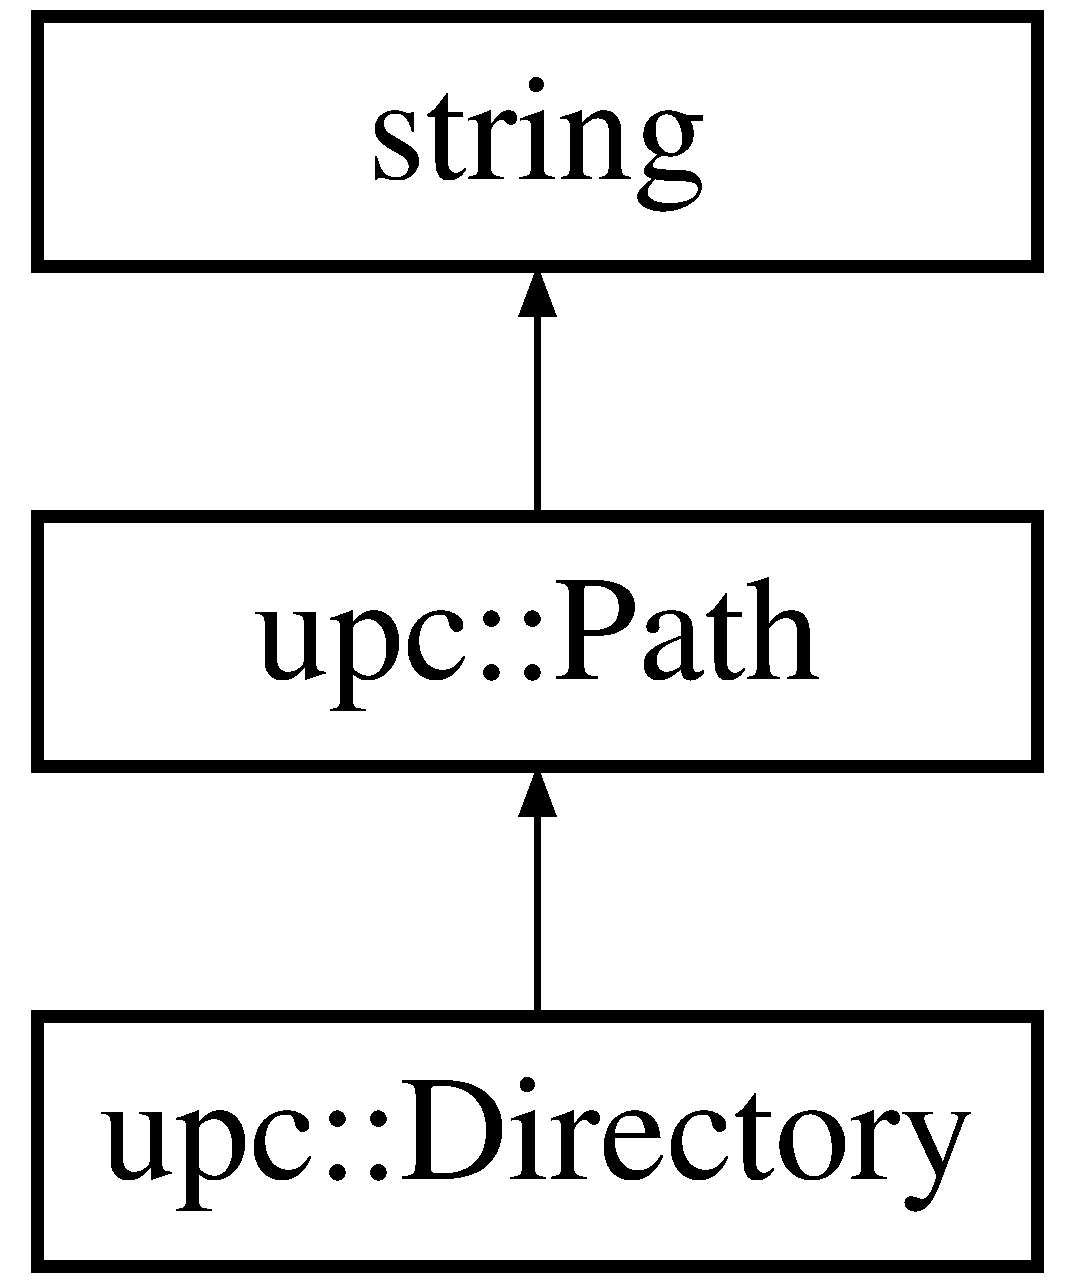
\includegraphics[height=3.000000cm]{classupc_1_1Directory}
\end{center}
\end{figure}
\subsection*{Public Member Functions}
\begin{DoxyCompactItemize}
\item 
\hyperlink{classupc_1_1Directory_a2b40221a7578b439c262c66ba964f6c2}{Directory} ()
\item 
\hyperlink{classupc_1_1Directory_a4b6321fb7644d3dcf225e2e666b837da}{Directory} (const \hyperlink{classupc_1_1Path}{Path} \&p)
\item 
\hyperlink{classupc_1_1Directory_aca9acc226940f166429185989023727f}{Directory} (const string \&p)
\item 
\hyperlink{classupc_1_1Directory_afb8c8e0bc50664d8505e0fa392f99657}{Directory} (const char $\ast$p)
\item 
bool \hyperlink{classupc_1_1Directory_aa2f4f4351b856d193eae61ea647151d4}{make} () const 
\item 
bool \hyperlink{classupc_1_1Directory_a08e6caef56b6ca56619de80260ea7a9c}{exist} () const 
\item 
virtual \hyperlink{classupc_1_1Directory_a543f3d4556bce36eee6a64e11678f68f}{$\sim$\+Directory} ()
\end{DoxyCompactItemize}


\subsection{Constructor \& Destructor Documentation}
\index{upc\+::\+Directory@{upc\+::\+Directory}!Directory@{Directory}}
\index{Directory@{Directory}!upc\+::\+Directory@{upc\+::\+Directory}}
\subsubsection[{\texorpdfstring{Directory()}{Directory()}}]{\setlength{\rightskip}{0pt plus 5cm}upc\+::\+Directory\+::\+Directory (
\begin{DoxyParamCaption}
{}
\end{DoxyParamCaption}
)\hspace{0.3cm}{\ttfamily [inline]}}\hypertarget{classupc_1_1Directory_a2b40221a7578b439c262c66ba964f6c2}{}\label{classupc_1_1Directory_a2b40221a7578b439c262c66ba964f6c2}
\index{upc\+::\+Directory@{upc\+::\+Directory}!Directory@{Directory}}
\index{Directory@{Directory}!upc\+::\+Directory@{upc\+::\+Directory}}
\subsubsection[{\texorpdfstring{Directory(const Path \&p)}{Directory(const Path &p)}}]{\setlength{\rightskip}{0pt plus 5cm}upc\+::\+Directory\+::\+Directory (
\begin{DoxyParamCaption}
\item[{const {\bf Path} \&}]{p}
\end{DoxyParamCaption}
)\hspace{0.3cm}{\ttfamily [inline]}}\hypertarget{classupc_1_1Directory_a4b6321fb7644d3dcf225e2e666b837da}{}\label{classupc_1_1Directory_a4b6321fb7644d3dcf225e2e666b837da}
\index{upc\+::\+Directory@{upc\+::\+Directory}!Directory@{Directory}}
\index{Directory@{Directory}!upc\+::\+Directory@{upc\+::\+Directory}}
\subsubsection[{\texorpdfstring{Directory(const string \&p)}{Directory(const string &p)}}]{\setlength{\rightskip}{0pt plus 5cm}upc\+::\+Directory\+::\+Directory (
\begin{DoxyParamCaption}
\item[{const string \&}]{p}
\end{DoxyParamCaption}
)\hspace{0.3cm}{\ttfamily [inline]}}\hypertarget{classupc_1_1Directory_aca9acc226940f166429185989023727f}{}\label{classupc_1_1Directory_aca9acc226940f166429185989023727f}
\index{upc\+::\+Directory@{upc\+::\+Directory}!Directory@{Directory}}
\index{Directory@{Directory}!upc\+::\+Directory@{upc\+::\+Directory}}
\subsubsection[{\texorpdfstring{Directory(const char $\ast$p)}{Directory(const char *p)}}]{\setlength{\rightskip}{0pt plus 5cm}upc\+::\+Directory\+::\+Directory (
\begin{DoxyParamCaption}
\item[{const char $\ast$}]{p}
\end{DoxyParamCaption}
)\hspace{0.3cm}{\ttfamily [inline]}}\hypertarget{classupc_1_1Directory_afb8c8e0bc50664d8505e0fa392f99657}{}\label{classupc_1_1Directory_afb8c8e0bc50664d8505e0fa392f99657}
\index{upc\+::\+Directory@{upc\+::\+Directory}!````~Directory@{$\sim$\+Directory}}
\index{````~Directory@{$\sim$\+Directory}!upc\+::\+Directory@{upc\+::\+Directory}}
\subsubsection[{\texorpdfstring{$\sim$\+Directory()}{~Directory()}}]{\setlength{\rightskip}{0pt plus 5cm}virtual upc\+::\+Directory\+::$\sim$\+Directory (
\begin{DoxyParamCaption}
{}
\end{DoxyParamCaption}
)\hspace{0.3cm}{\ttfamily [inline]}, {\ttfamily [virtual]}}\hypertarget{classupc_1_1Directory_a543f3d4556bce36eee6a64e11678f68f}{}\label{classupc_1_1Directory_a543f3d4556bce36eee6a64e11678f68f}


\subsection{Member Function Documentation}
\index{upc\+::\+Directory@{upc\+::\+Directory}!exist@{exist}}
\index{exist@{exist}!upc\+::\+Directory@{upc\+::\+Directory}}
\subsubsection[{\texorpdfstring{exist() const }{exist() const }}]{\setlength{\rightskip}{0pt plus 5cm}bool upc\+::\+Directory\+::exist (
\begin{DoxyParamCaption}
{}
\end{DoxyParamCaption}
) const}\hypertarget{classupc_1_1Directory_a08e6caef56b6ca56619de80260ea7a9c}{}\label{classupc_1_1Directory_a08e6caef56b6ca56619de80260ea7a9c}
\index{upc\+::\+Directory@{upc\+::\+Directory}!make@{make}}
\index{make@{make}!upc\+::\+Directory@{upc\+::\+Directory}}
\subsubsection[{\texorpdfstring{make() const }{make() const }}]{\setlength{\rightskip}{0pt plus 5cm}bool upc\+::\+Directory\+::make (
\begin{DoxyParamCaption}
{}
\end{DoxyParamCaption}
) const}\hypertarget{classupc_1_1Directory_aa2f4f4351b856d193eae61ea647151d4}{}\label{classupc_1_1Directory_aa2f4f4351b856d193eae61ea647151d4}


The documentation for this class was generated from the following files\+:\begin{DoxyCompactItemize}
\item 
include/\hyperlink{filename_8h}{filename.\+h}\item 
pav/\hyperlink{filename_8cpp}{filename.\+cpp}\end{DoxyCompactItemize}

\hypertarget{classffft_1_1DynArray}{}\section{ffft\+:\+:Dyn\+Array$<$ T $>$ Class Template Reference}
\label{classffft_1_1DynArray}\index{ffft\+::\+Dyn\+Array$<$ T $>$@{ffft\+::\+Dyn\+Array$<$ T $>$}}


{\ttfamily \#include $<$Dyn\+Array.\+h$>$}

\subsection*{Public Types}
\begin{DoxyCompactItemize}
\item 
typedef T \hyperlink{classffft_1_1DynArray_aa21fa88c73e511acb18a7e778190ab02}{Data\+Type}
\end{DoxyCompactItemize}
\subsection*{Public Member Functions}
\begin{DoxyCompactItemize}
\item 
\hyperlink{classffft_1_1DynArray_a3a1bc9474a3891360464c4ad97d846ff}{Dyn\+Array} ()
\item 
\hyperlink{classffft_1_1DynArray_a26919351a30b4be36c3e3ee500a7c6a7}{Dyn\+Array} (long \hyperlink{classffft_1_1DynArray_aab5a878741b62b079c94db354357127d}{size})
\item 
\hyperlink{classffft_1_1DynArray_a0467340a0c0b5cbb47683c665e21ffd6}{$\sim$\+Dyn\+Array} ()
\item 
long \hyperlink{classffft_1_1DynArray_aab5a878741b62b079c94db354357127d}{size} () const 
\item 
void \hyperlink{classffft_1_1DynArray_a3879167bca7e35ee75596318f67e2930}{resize} (long \hyperlink{classffft_1_1DynArray_aab5a878741b62b079c94db354357127d}{size})
\item 
const \hyperlink{classffft_1_1DynArray_aa21fa88c73e511acb18a7e778190ab02}{Data\+Type} \& \hyperlink{classffft_1_1DynArray_a502aab733f04c8fed33348bce9f49e92}{operator\mbox{[}$\,$\mbox{]}} (long pos) const 
\item 
\hyperlink{classffft_1_1DynArray_aa21fa88c73e511acb18a7e778190ab02}{Data\+Type} \& \hyperlink{classffft_1_1DynArray_a79c769ea7c52d0fbbe67831380b9a89c}{operator\mbox{[}$\,$\mbox{]}} (long pos)
\end{DoxyCompactItemize}
\subsection*{Private Member Functions}
\begin{DoxyCompactItemize}
\item 
\hyperlink{classffft_1_1DynArray_a7d28eb73cf75f2c669a32dde120eb2cb}{Dyn\+Array} (const \hyperlink{classffft_1_1DynArray}{Dyn\+Array} \&other)
\item 
\hyperlink{classffft_1_1DynArray}{Dyn\+Array} \& \hyperlink{classffft_1_1DynArray_ab16be271312566a8ba4d2867ae2a1e5e}{operator=} (const \hyperlink{classffft_1_1DynArray}{Dyn\+Array} \&other)
\item 
bool \hyperlink{classffft_1_1DynArray_a7418a4e9990dc57b076ed5b21b1483a0}{operator==} (const \hyperlink{classffft_1_1DynArray}{Dyn\+Array} \&other)
\item 
bool \hyperlink{classffft_1_1DynArray_afe1e0c664bde31b145b3782817e355fd}{operator!=} (const \hyperlink{classffft_1_1DynArray}{Dyn\+Array} \&other)
\end{DoxyCompactItemize}
\subsection*{Private Attributes}
\begin{DoxyCompactItemize}
\item 
\hyperlink{classffft_1_1DynArray_aa21fa88c73e511acb18a7e778190ab02}{Data\+Type} $\ast$ \hyperlink{classffft_1_1DynArray_acfb894fb97f7a2aed0e5c242bb82073a}{\+\_\+data\+\_\+ptr}
\item 
long \hyperlink{classffft_1_1DynArray_ab598085ccf8352effe43635aec134cb6}{\+\_\+len}
\end{DoxyCompactItemize}


\subsection{Member Typedef Documentation}
\index{ffft\+::\+Dyn\+Array@{ffft\+::\+Dyn\+Array}!Data\+Type@{Data\+Type}}
\index{Data\+Type@{Data\+Type}!ffft\+::\+Dyn\+Array@{ffft\+::\+Dyn\+Array}}
\subsubsection[{\texorpdfstring{Data\+Type}{DataType}}]{\setlength{\rightskip}{0pt plus 5cm}template$<$class T$>$ typedef T {\bf ffft\+::\+Dyn\+Array}$<$ T $>$\+::{\bf Data\+Type}}\hypertarget{classffft_1_1DynArray_aa21fa88c73e511acb18a7e778190ab02}{}\label{classffft_1_1DynArray_aa21fa88c73e511acb18a7e778190ab02}


\subsection{Constructor \& Destructor Documentation}
\index{ffft\+::\+Dyn\+Array@{ffft\+::\+Dyn\+Array}!Dyn\+Array@{Dyn\+Array}}
\index{Dyn\+Array@{Dyn\+Array}!ffft\+::\+Dyn\+Array@{ffft\+::\+Dyn\+Array}}
\subsubsection[{\texorpdfstring{Dyn\+Array()}{DynArray()}}]{\setlength{\rightskip}{0pt plus 5cm}template$<$class T $>$ {\bf ffft\+::\+Dyn\+Array}$<$ T $>$\+::{\bf Dyn\+Array} (
\begin{DoxyParamCaption}
{}
\end{DoxyParamCaption}
)}\hypertarget{classffft_1_1DynArray_a3a1bc9474a3891360464c4ad97d846ff}{}\label{classffft_1_1DynArray_a3a1bc9474a3891360464c4ad97d846ff}
\index{ffft\+::\+Dyn\+Array@{ffft\+::\+Dyn\+Array}!Dyn\+Array@{Dyn\+Array}}
\index{Dyn\+Array@{Dyn\+Array}!ffft\+::\+Dyn\+Array@{ffft\+::\+Dyn\+Array}}
\subsubsection[{\texorpdfstring{Dyn\+Array(long size)}{DynArray(long size)}}]{\setlength{\rightskip}{0pt plus 5cm}template$<$class T $>$ {\bf ffft\+::\+Dyn\+Array}$<$ T $>$\+::{\bf Dyn\+Array} (
\begin{DoxyParamCaption}
\item[{long}]{size}
\end{DoxyParamCaption}
)\hspace{0.3cm}{\ttfamily [explicit]}}\hypertarget{classffft_1_1DynArray_a26919351a30b4be36c3e3ee500a7c6a7}{}\label{classffft_1_1DynArray_a26919351a30b4be36c3e3ee500a7c6a7}
\index{ffft\+::\+Dyn\+Array@{ffft\+::\+Dyn\+Array}!````~Dyn\+Array@{$\sim$\+Dyn\+Array}}
\index{````~Dyn\+Array@{$\sim$\+Dyn\+Array}!ffft\+::\+Dyn\+Array@{ffft\+::\+Dyn\+Array}}
\subsubsection[{\texorpdfstring{$\sim$\+Dyn\+Array()}{~DynArray()}}]{\setlength{\rightskip}{0pt plus 5cm}template$<$class T $>$ {\bf ffft\+::\+Dyn\+Array}$<$ T $>$\+::$\sim${\bf Dyn\+Array} (
\begin{DoxyParamCaption}
{}
\end{DoxyParamCaption}
)}\hypertarget{classffft_1_1DynArray_a0467340a0c0b5cbb47683c665e21ffd6}{}\label{classffft_1_1DynArray_a0467340a0c0b5cbb47683c665e21ffd6}
\index{ffft\+::\+Dyn\+Array@{ffft\+::\+Dyn\+Array}!Dyn\+Array@{Dyn\+Array}}
\index{Dyn\+Array@{Dyn\+Array}!ffft\+::\+Dyn\+Array@{ffft\+::\+Dyn\+Array}}
\subsubsection[{\texorpdfstring{Dyn\+Array(const Dyn\+Array \&other)}{DynArray(const DynArray &other)}}]{\setlength{\rightskip}{0pt plus 5cm}template$<$class T$>$ {\bf ffft\+::\+Dyn\+Array}$<$ T $>$\+::{\bf Dyn\+Array} (
\begin{DoxyParamCaption}
\item[{const {\bf Dyn\+Array}$<$ T $>$ \&}]{other}
\end{DoxyParamCaption}
)\hspace{0.3cm}{\ttfamily [private]}}\hypertarget{classffft_1_1DynArray_a7d28eb73cf75f2c669a32dde120eb2cb}{}\label{classffft_1_1DynArray_a7d28eb73cf75f2c669a32dde120eb2cb}


\subsection{Member Function Documentation}
\index{ffft\+::\+Dyn\+Array@{ffft\+::\+Dyn\+Array}!operator"!=@{operator"!=}}
\index{operator"!=@{operator"!=}!ffft\+::\+Dyn\+Array@{ffft\+::\+Dyn\+Array}}
\subsubsection[{\texorpdfstring{operator"!=(const Dyn\+Array \&other)}{operator!=(const DynArray &other)}}]{\setlength{\rightskip}{0pt plus 5cm}template$<$class T$>$ bool {\bf ffft\+::\+Dyn\+Array}$<$ T $>$\+::operator!= (
\begin{DoxyParamCaption}
\item[{const {\bf Dyn\+Array}$<$ T $>$ \&}]{other}
\end{DoxyParamCaption}
)\hspace{0.3cm}{\ttfamily [private]}}\hypertarget{classffft_1_1DynArray_afe1e0c664bde31b145b3782817e355fd}{}\label{classffft_1_1DynArray_afe1e0c664bde31b145b3782817e355fd}
\index{ffft\+::\+Dyn\+Array@{ffft\+::\+Dyn\+Array}!operator=@{operator=}}
\index{operator=@{operator=}!ffft\+::\+Dyn\+Array@{ffft\+::\+Dyn\+Array}}
\subsubsection[{\texorpdfstring{operator=(const Dyn\+Array \&other)}{operator=(const DynArray &other)}}]{\setlength{\rightskip}{0pt plus 5cm}template$<$class T$>$ {\bf Dyn\+Array}\& {\bf ffft\+::\+Dyn\+Array}$<$ T $>$\+::operator= (
\begin{DoxyParamCaption}
\item[{const {\bf Dyn\+Array}$<$ T $>$ \&}]{other}
\end{DoxyParamCaption}
)\hspace{0.3cm}{\ttfamily [private]}}\hypertarget{classffft_1_1DynArray_ab16be271312566a8ba4d2867ae2a1e5e}{}\label{classffft_1_1DynArray_ab16be271312566a8ba4d2867ae2a1e5e}
\index{ffft\+::\+Dyn\+Array@{ffft\+::\+Dyn\+Array}!operator==@{operator==}}
\index{operator==@{operator==}!ffft\+::\+Dyn\+Array@{ffft\+::\+Dyn\+Array}}
\subsubsection[{\texorpdfstring{operator==(const Dyn\+Array \&other)}{operator==(const DynArray &other)}}]{\setlength{\rightskip}{0pt plus 5cm}template$<$class T$>$ bool {\bf ffft\+::\+Dyn\+Array}$<$ T $>$\+::operator== (
\begin{DoxyParamCaption}
\item[{const {\bf Dyn\+Array}$<$ T $>$ \&}]{other}
\end{DoxyParamCaption}
)\hspace{0.3cm}{\ttfamily [private]}}\hypertarget{classffft_1_1DynArray_a7418a4e9990dc57b076ed5b21b1483a0}{}\label{classffft_1_1DynArray_a7418a4e9990dc57b076ed5b21b1483a0}
\index{ffft\+::\+Dyn\+Array@{ffft\+::\+Dyn\+Array}!operator\mbox{[}$\,$\mbox{]}@{operator[]}}
\index{operator\mbox{[}$\,$\mbox{]}@{operator[]}!ffft\+::\+Dyn\+Array@{ffft\+::\+Dyn\+Array}}
\subsubsection[{\texorpdfstring{operator[](long pos) const }{operator[](long pos) const }}]{\setlength{\rightskip}{0pt plus 5cm}template$<$class T $>$ const {\bf Dyn\+Array}$<$ T $>$\+::{\bf Data\+Type} \& {\bf ffft\+::\+Dyn\+Array}$<$ T $>$\+::operator\mbox{[}$\,$\mbox{]} (
\begin{DoxyParamCaption}
\item[{long}]{pos}
\end{DoxyParamCaption}
) const\hspace{0.3cm}{\ttfamily [inline]}}\hypertarget{classffft_1_1DynArray_a502aab733f04c8fed33348bce9f49e92}{}\label{classffft_1_1DynArray_a502aab733f04c8fed33348bce9f49e92}
\index{ffft\+::\+Dyn\+Array@{ffft\+::\+Dyn\+Array}!operator\mbox{[}$\,$\mbox{]}@{operator[]}}
\index{operator\mbox{[}$\,$\mbox{]}@{operator[]}!ffft\+::\+Dyn\+Array@{ffft\+::\+Dyn\+Array}}
\subsubsection[{\texorpdfstring{operator[](long pos)}{operator[](long pos)}}]{\setlength{\rightskip}{0pt plus 5cm}template$<$class T $>$ {\bf Dyn\+Array}$<$ T $>$\+::{\bf Data\+Type} \& {\bf ffft\+::\+Dyn\+Array}$<$ T $>$\+::operator\mbox{[}$\,$\mbox{]} (
\begin{DoxyParamCaption}
\item[{long}]{pos}
\end{DoxyParamCaption}
)\hspace{0.3cm}{\ttfamily [inline]}}\hypertarget{classffft_1_1DynArray_a79c769ea7c52d0fbbe67831380b9a89c}{}\label{classffft_1_1DynArray_a79c769ea7c52d0fbbe67831380b9a89c}
\index{ffft\+::\+Dyn\+Array@{ffft\+::\+Dyn\+Array}!resize@{resize}}
\index{resize@{resize}!ffft\+::\+Dyn\+Array@{ffft\+::\+Dyn\+Array}}
\subsubsection[{\texorpdfstring{resize(long size)}{resize(long size)}}]{\setlength{\rightskip}{0pt plus 5cm}template$<$class T $>$ void {\bf ffft\+::\+Dyn\+Array}$<$ T $>$\+::resize (
\begin{DoxyParamCaption}
\item[{long}]{size}
\end{DoxyParamCaption}
)\hspace{0.3cm}{\ttfamily [inline]}}\hypertarget{classffft_1_1DynArray_a3879167bca7e35ee75596318f67e2930}{}\label{classffft_1_1DynArray_a3879167bca7e35ee75596318f67e2930}
\index{ffft\+::\+Dyn\+Array@{ffft\+::\+Dyn\+Array}!size@{size}}
\index{size@{size}!ffft\+::\+Dyn\+Array@{ffft\+::\+Dyn\+Array}}
\subsubsection[{\texorpdfstring{size() const }{size() const }}]{\setlength{\rightskip}{0pt plus 5cm}template$<$class T $>$ long {\bf ffft\+::\+Dyn\+Array}$<$ T $>$\+::size (
\begin{DoxyParamCaption}
{}
\end{DoxyParamCaption}
) const\hspace{0.3cm}{\ttfamily [inline]}}\hypertarget{classffft_1_1DynArray_aab5a878741b62b079c94db354357127d}{}\label{classffft_1_1DynArray_aab5a878741b62b079c94db354357127d}


\subsection{Member Data Documentation}
\index{ffft\+::\+Dyn\+Array@{ffft\+::\+Dyn\+Array}!\+\_\+data\+\_\+ptr@{\+\_\+data\+\_\+ptr}}
\index{\+\_\+data\+\_\+ptr@{\+\_\+data\+\_\+ptr}!ffft\+::\+Dyn\+Array@{ffft\+::\+Dyn\+Array}}
\subsubsection[{\texorpdfstring{\+\_\+data\+\_\+ptr}{_data_ptr}}]{\setlength{\rightskip}{0pt plus 5cm}template$<$class T$>$ {\bf Data\+Type}$\ast$ {\bf ffft\+::\+Dyn\+Array}$<$ T $>$\+::\+\_\+data\+\_\+ptr\hspace{0.3cm}{\ttfamily [private]}}\hypertarget{classffft_1_1DynArray_acfb894fb97f7a2aed0e5c242bb82073a}{}\label{classffft_1_1DynArray_acfb894fb97f7a2aed0e5c242bb82073a}
\index{ffft\+::\+Dyn\+Array@{ffft\+::\+Dyn\+Array}!\+\_\+len@{\+\_\+len}}
\index{\+\_\+len@{\+\_\+len}!ffft\+::\+Dyn\+Array@{ffft\+::\+Dyn\+Array}}
\subsubsection[{\texorpdfstring{\+\_\+len}{_len}}]{\setlength{\rightskip}{0pt plus 5cm}template$<$class T$>$ long {\bf ffft\+::\+Dyn\+Array}$<$ T $>$\+::\+\_\+len\hspace{0.3cm}{\ttfamily [private]}}\hypertarget{classffft_1_1DynArray_ab598085ccf8352effe43635aec134cb6}{}\label{classffft_1_1DynArray_ab598085ccf8352effe43635aec134cb6}


The documentation for this class was generated from the following files\+:\begin{DoxyCompactItemize}
\item 
include/ffft/\hyperlink{DynArray_8h}{Dyn\+Array.\+h}\item 
include/ffft/\hyperlink{DynArray_8hpp}{Dyn\+Array.\+hpp}\end{DoxyCompactItemize}

\hypertarget{classupc_1_1Ext}{}\section{upc\+:\+:Ext Class Reference}
\label{classupc_1_1Ext}\index{upc\+::\+Ext@{upc\+::\+Ext}}


{\ttfamily \#include $<$filename.\+h$>$}

Inheritance diagram for upc\+:\+:Ext\+:\begin{figure}[H]
\begin{center}
\leavevmode
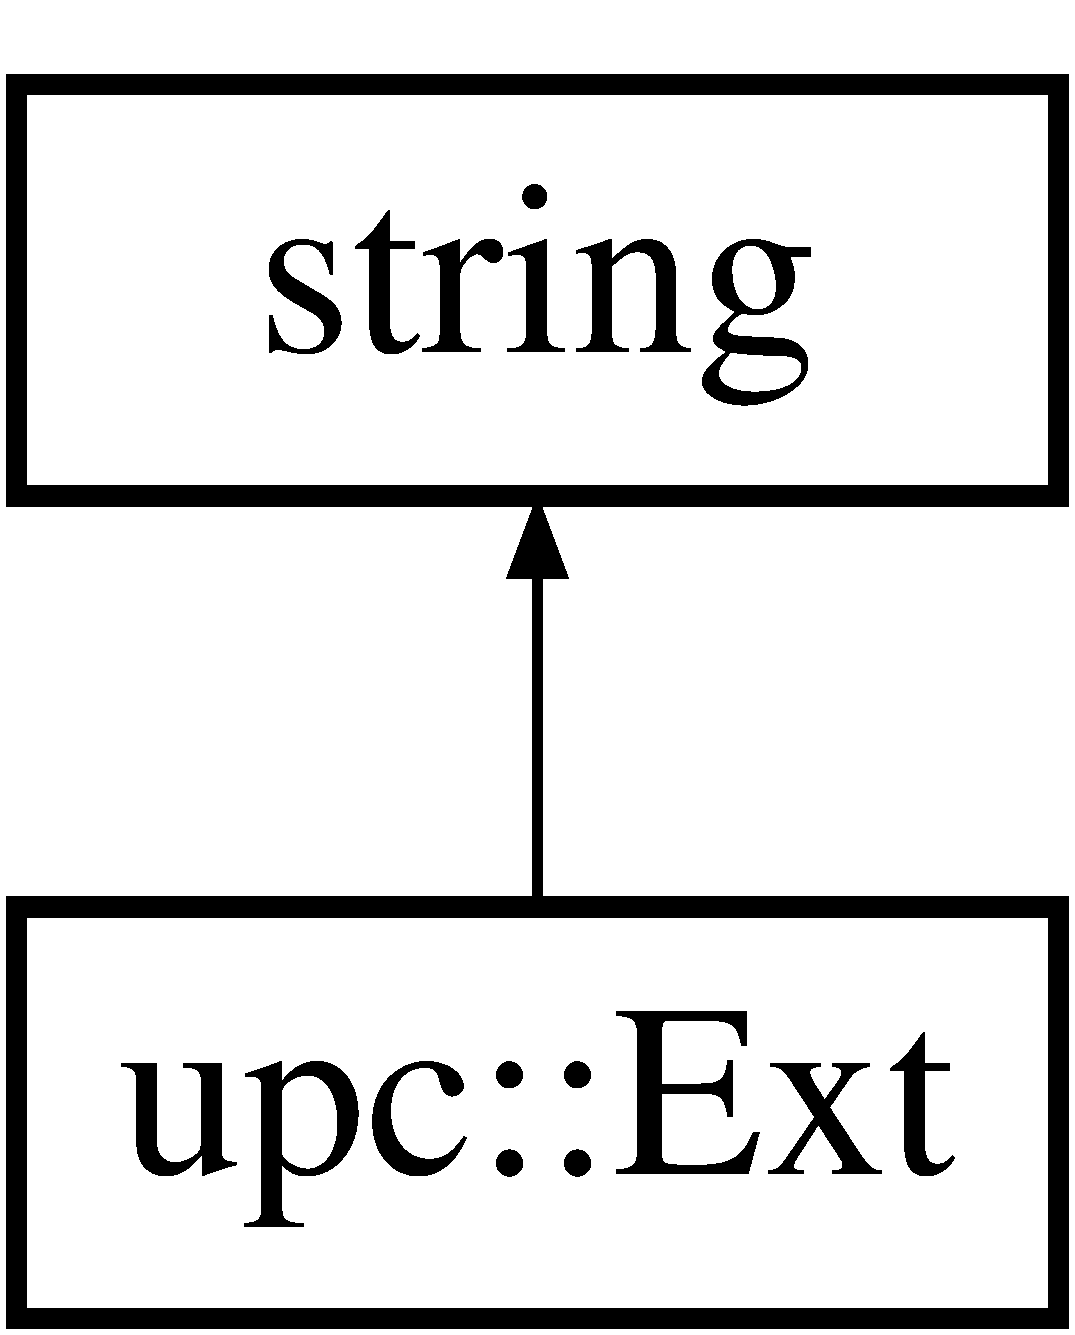
\includegraphics[height=2.000000cm]{classupc_1_1Ext}
\end{center}
\end{figure}
\subsection*{Public Member Functions}
\begin{DoxyCompactItemize}
\item 
\hyperlink{classupc_1_1Ext_af9636b92ecb5e6f5d0f16ae4d968c21a}{Ext} (const string \&str)
\item 
\hyperlink{classupc_1_1Ext_a0e3b4b899d14b0bef3dbf566a38086ae}{Ext} (const char $\ast$str)
\end{DoxyCompactItemize}
\subsection*{Private Member Functions}
\begin{DoxyCompactItemize}
\item 
void \hyperlink{classupc_1_1Ext_a05030fdcb67a89c115bc965a44164ea0}{check\+\_\+dot} ()
\end{DoxyCompactItemize}


\subsection{Constructor \& Destructor Documentation}
\index{upc\+::\+Ext@{upc\+::\+Ext}!Ext@{Ext}}
\index{Ext@{Ext}!upc\+::\+Ext@{upc\+::\+Ext}}
\subsubsection[{\texorpdfstring{Ext(const string \&str)}{Ext(const string &str)}}]{\setlength{\rightskip}{0pt plus 5cm}upc\+::\+Ext\+::\+Ext (
\begin{DoxyParamCaption}
\item[{const string \&}]{str}
\end{DoxyParamCaption}
)\hspace{0.3cm}{\ttfamily [inline]}}\hypertarget{classupc_1_1Ext_af9636b92ecb5e6f5d0f16ae4d968c21a}{}\label{classupc_1_1Ext_af9636b92ecb5e6f5d0f16ae4d968c21a}
\index{upc\+::\+Ext@{upc\+::\+Ext}!Ext@{Ext}}
\index{Ext@{Ext}!upc\+::\+Ext@{upc\+::\+Ext}}
\subsubsection[{\texorpdfstring{Ext(const char $\ast$str)}{Ext(const char *str)}}]{\setlength{\rightskip}{0pt plus 5cm}upc\+::\+Ext\+::\+Ext (
\begin{DoxyParamCaption}
\item[{const char $\ast$}]{str}
\end{DoxyParamCaption}
)\hspace{0.3cm}{\ttfamily [inline]}}\hypertarget{classupc_1_1Ext_a0e3b4b899d14b0bef3dbf566a38086ae}{}\label{classupc_1_1Ext_a0e3b4b899d14b0bef3dbf566a38086ae}


\subsection{Member Function Documentation}
\index{upc\+::\+Ext@{upc\+::\+Ext}!check\+\_\+dot@{check\+\_\+dot}}
\index{check\+\_\+dot@{check\+\_\+dot}!upc\+::\+Ext@{upc\+::\+Ext}}
\subsubsection[{\texorpdfstring{check\+\_\+dot()}{check_dot()}}]{\setlength{\rightskip}{0pt plus 5cm}void upc\+::\+Ext\+::check\+\_\+dot (
\begin{DoxyParamCaption}
{}
\end{DoxyParamCaption}
)\hspace{0.3cm}{\ttfamily [inline]}, {\ttfamily [private]}}\hypertarget{classupc_1_1Ext_a05030fdcb67a89c115bc965a44164ea0}{}\label{classupc_1_1Ext_a05030fdcb67a89c115bc965a44164ea0}


The documentation for this class was generated from the following file\+:\begin{DoxyCompactItemize}
\item 
include/\hyperlink{filename_8h}{filename.\+h}\end{DoxyCompactItemize}

\hypertarget{structFeatures}{}\section{Features Struct Reference}
\label{structFeatures}\index{Features@{Features}}
\subsection*{Public Attributes}
\begin{DoxyCompactItemize}
\item 
\hyperlink{FFTReal__readme_8txt_a0ea2fae2a8106200bf378b90eae003cf}{float} \hyperlink{structFeatures_a02006441e52641420bcac6b7adffc660}{zcr}
\item 
\hyperlink{FFTReal__readme_8txt_a0ea2fae2a8106200bf378b90eae003cf}{float} \hyperlink{structFeatures_a7ab66b5f9a14d82c41e411873d3ef425}{p}
\item 
\hyperlink{FFTReal__readme_8txt_a0ea2fae2a8106200bf378b90eae003cf}{float} \hyperlink{structFeatures_a767255b0011e02ba7edc937e69805dd4}{am}
\end{DoxyCompactItemize}


\subsection{Member Data Documentation}
\index{Features@{Features}!am@{am}}
\index{am@{am}!Features@{Features}}
\subsubsection[{\texorpdfstring{am}{am}}]{\setlength{\rightskip}{0pt plus 5cm}{\bf float} Features\+::am}\hypertarget{structFeatures_a767255b0011e02ba7edc937e69805dd4}{}\label{structFeatures_a767255b0011e02ba7edc937e69805dd4}
\index{Features@{Features}!p@{p}}
\index{p@{p}!Features@{Features}}
\subsubsection[{\texorpdfstring{p}{p}}]{\setlength{\rightskip}{0pt plus 5cm}{\bf float} Features\+::p}\hypertarget{structFeatures_a7ab66b5f9a14d82c41e411873d3ef425}{}\label{structFeatures_a7ab66b5f9a14d82c41e411873d3ef425}
\index{Features@{Features}!zcr@{zcr}}
\index{zcr@{zcr}!Features@{Features}}
\subsubsection[{\texorpdfstring{zcr}{zcr}}]{\setlength{\rightskip}{0pt plus 5cm}{\bf float} Features\+::zcr}\hypertarget{structFeatures_a02006441e52641420bcac6b7adffc660}{}\label{structFeatures_a02006441e52641420bcac6b7adffc660}


The documentation for this struct was generated from the following file\+:\begin{DoxyCompactItemize}
\item 
pav/\hyperlink{vad_8c}{vad.\+c}\end{DoxyCompactItemize}

\hypertarget{classffft_1_1FFTReal}{}\section{ffft\+:\+:F\+F\+T\+Real$<$ DT $>$ Class Template Reference}
\label{classffft_1_1FFTReal}\index{ffft\+::\+F\+F\+T\+Real$<$ D\+T $>$@{ffft\+::\+F\+F\+T\+Real$<$ D\+T $>$}}


{\ttfamily \#include $<$F\+F\+T\+Real.\+h$>$}

\subsection*{Public Types}
\begin{DoxyCompactItemize}
\item 
enum \{ \hyperlink{classffft_1_1FFTReal_a39f5a2ec14c15f9198268500716e5dbaabec37ae38b07b6e3e1230562f01882a2}{M\+A\+X\+\_\+\+B\+I\+T\+\_\+\+D\+E\+P\+TH} = 30
 \}
\item 
typedef DT \hyperlink{classffft_1_1FFTReal_a606148f1cf8c3b7d705473932fc063d1}{Data\+Type}
\end{DoxyCompactItemize}
\subsection*{Public Member Functions}
\begin{DoxyCompactItemize}
\item 
\hyperlink{classffft_1_1FFTReal_a627db4d781235302c3a229fc4d7a10ba}{F\+F\+T\+Real} (long length)
\item 
virtual \hyperlink{classffft_1_1FFTReal_a04f14f3576aac18af45ba22c38fbaf2a}{$\sim$\+F\+F\+T\+Real} ()
\item 
long \hyperlink{classffft_1_1FFTReal_abdd5b144ba5737c7ad27095d1658c29e}{get\+\_\+length} () const 
\item 
void \hyperlink{classffft_1_1FFTReal_a4c5b863a285c5a87f38517735cbf1352}{do\+\_\+fft} (\hyperlink{classffft_1_1FFTReal_a606148f1cf8c3b7d705473932fc063d1}{Data\+Type} \hyperlink{FFTReal__readme_8txt_abbf3cc73d1e3e4714ab1639819396eca}{f}\mbox{[}$\,$\mbox{]}, const \hyperlink{classffft_1_1FFTReal_a606148f1cf8c3b7d705473932fc063d1}{Data\+Type} \hyperlink{FFTReal__readme_8txt_a9c92ac89d1560f812393ca39a19e581e}{x}\mbox{[}$\,$\mbox{]}) const 
\item 
void \hyperlink{classffft_1_1FFTReal_a8ab2e0da482cea88a61f01d58c074989}{do\+\_\+ifft} (const \hyperlink{classffft_1_1FFTReal_a606148f1cf8c3b7d705473932fc063d1}{Data\+Type} \hyperlink{FFTReal__readme_8txt_abbf3cc73d1e3e4714ab1639819396eca}{f}\mbox{[}$\,$\mbox{]}, \hyperlink{classffft_1_1FFTReal_a606148f1cf8c3b7d705473932fc063d1}{Data\+Type} \hyperlink{FFTReal__readme_8txt_a9c92ac89d1560f812393ca39a19e581e}{x}\mbox{[}$\,$\mbox{]}) const 
\item 
void \hyperlink{classffft_1_1FFTReal_a9e30fff775905b1059aa9299004ee228}{rescale} (\hyperlink{classffft_1_1FFTReal_a606148f1cf8c3b7d705473932fc063d1}{Data\+Type} \hyperlink{FFTReal__readme_8txt_a9c92ac89d1560f812393ca39a19e581e}{x}\mbox{[}$\,$\mbox{]}) const 
\item 
\hyperlink{classffft_1_1FFTReal_a606148f1cf8c3b7d705473932fc063d1}{Data\+Type} $\ast$ \hyperlink{classffft_1_1FFTReal_af1fcd007f1cf0b41bd2188e0b3cd5cca}{use\+\_\+buffer} () const 
\end{DoxyCompactItemize}
\subsection*{Private Types}
\begin{DoxyCompactItemize}
\item 
enum \{ \hyperlink{classffft_1_1FFTReal_a69a4ed5b7507683f5233ddbd34f0e1eea5b9b73ce99dfec1ae2f92dd0151fa07e}{T\+R\+I\+G\+O\+\_\+\+B\+D\+\_\+\+L\+I\+M\+IT} = 12
 \}
\item 
typedef \hyperlink{classffft_1_1OscSinCos}{Osc\+Sin\+Cos}$<$ \hyperlink{classffft_1_1FFTReal_a606148f1cf8c3b7d705473932fc063d1}{Data\+Type} $>$ \hyperlink{classffft_1_1FFTReal_a3b9f6dae05435b3696c6c84155e0953a}{Osc\+Type}
\end{DoxyCompactItemize}
\subsection*{Private Member Functions}
\begin{DoxyCompactItemize}
\item 
void \hyperlink{classffft_1_1FFTReal_aa7315c1c287185277a8188eb4c6180c8}{init\+\_\+br\+\_\+lut} ()
\item 
void \hyperlink{classffft_1_1FFTReal_aac5c6c408da94a9d346e97aeded61ef2}{init\+\_\+trigo\+\_\+lut} ()
\item 
void \hyperlink{classffft_1_1FFTReal_adcac1258791df06ea6597c7f4fc49f63}{init\+\_\+trigo\+\_\+osc} ()
\item 
\hyperlink{def_8h_a31b2ada863c9efa7455efae4e13661f3}{ffft\+\_\+\+F\+O\+R\+C\+E\+I\+N\+L\+I\+NE} const long $\ast$ \hyperlink{classffft_1_1FFTReal_ae8bd596a64bbc6ff19a1b7efe0da50bc}{get\+\_\+br\+\_\+ptr} () const 
\item 
\hyperlink{def_8h_a31b2ada863c9efa7455efae4e13661f3}{ffft\+\_\+\+F\+O\+R\+C\+E\+I\+N\+L\+I\+NE} const \hyperlink{classffft_1_1FFTReal_a606148f1cf8c3b7d705473932fc063d1}{Data\+Type} $\ast$ \hyperlink{classffft_1_1FFTReal_a9683286954e4f26259af2c0f5c8727cb}{get\+\_\+trigo\+\_\+ptr} (int level) const 
\item 
\hyperlink{def_8h_a31b2ada863c9efa7455efae4e13661f3}{ffft\+\_\+\+F\+O\+R\+C\+E\+I\+N\+L\+I\+NE} long \hyperlink{classffft_1_1FFTReal_ae99a3872cc7dafca94190ee0d0e50fec}{get\+\_\+trigo\+\_\+level\+\_\+index} (int level) const 
\item 
void \hyperlink{classffft_1_1FFTReal_afdaf4c3d2ccb9fffcaa7d686179dd9ff}{compute\+\_\+fft\+\_\+general} (\hyperlink{classffft_1_1FFTReal_a606148f1cf8c3b7d705473932fc063d1}{Data\+Type} \hyperlink{FFTReal__readme_8txt_abbf3cc73d1e3e4714ab1639819396eca}{f}\mbox{[}$\,$\mbox{]}, const \hyperlink{classffft_1_1FFTReal_a606148f1cf8c3b7d705473932fc063d1}{Data\+Type} \hyperlink{FFTReal__readme_8txt_a9c92ac89d1560f812393ca39a19e581e}{x}\mbox{[}$\,$\mbox{]}) const 
\item 
void \hyperlink{classffft_1_1FFTReal_ac68be02ec38a22046a95a9b844da25db}{compute\+\_\+direct\+\_\+pass\+\_\+1\+\_\+2} (\hyperlink{classffft_1_1FFTReal_a606148f1cf8c3b7d705473932fc063d1}{Data\+Type} df\mbox{[}$\,$\mbox{]}, const \hyperlink{classffft_1_1FFTReal_a606148f1cf8c3b7d705473932fc063d1}{Data\+Type} \hyperlink{FFTReal__readme_8txt_a9c92ac89d1560f812393ca39a19e581e}{x}\mbox{[}$\,$\mbox{]}) const 
\item 
void \hyperlink{classffft_1_1FFTReal_a56b30d8e3cc4b343ea59cdaa54f326cd}{compute\+\_\+direct\+\_\+pass\+\_\+3} (\hyperlink{classffft_1_1FFTReal_a606148f1cf8c3b7d705473932fc063d1}{Data\+Type} df\mbox{[}$\,$\mbox{]}, const \hyperlink{classffft_1_1FFTReal_a606148f1cf8c3b7d705473932fc063d1}{Data\+Type} sf\mbox{[}$\,$\mbox{]}) const 
\item 
void \hyperlink{classffft_1_1FFTReal_a9ac801815332d3abd86ff1d7703f07e3}{compute\+\_\+direct\+\_\+pass\+\_\+n} (\hyperlink{classffft_1_1FFTReal_a606148f1cf8c3b7d705473932fc063d1}{Data\+Type} df\mbox{[}$\,$\mbox{]}, const \hyperlink{classffft_1_1FFTReal_a606148f1cf8c3b7d705473932fc063d1}{Data\+Type} sf\mbox{[}$\,$\mbox{]}, int pass) const 
\item 
void \hyperlink{classffft_1_1FFTReal_a91a4417bf6cff9a6af23f8538675a885}{compute\+\_\+direct\+\_\+pass\+\_\+n\+\_\+lut} (\hyperlink{classffft_1_1FFTReal_a606148f1cf8c3b7d705473932fc063d1}{Data\+Type} df\mbox{[}$\,$\mbox{]}, const \hyperlink{classffft_1_1FFTReal_a606148f1cf8c3b7d705473932fc063d1}{Data\+Type} sf\mbox{[}$\,$\mbox{]}, int pass) const 
\item 
void \hyperlink{classffft_1_1FFTReal_a388e0b14379bf9bf2c4e182713fee311}{compute\+\_\+direct\+\_\+pass\+\_\+n\+\_\+osc} (\hyperlink{classffft_1_1FFTReal_a606148f1cf8c3b7d705473932fc063d1}{Data\+Type} df\mbox{[}$\,$\mbox{]}, const \hyperlink{classffft_1_1FFTReal_a606148f1cf8c3b7d705473932fc063d1}{Data\+Type} sf\mbox{[}$\,$\mbox{]}, int pass) const 
\item 
void \hyperlink{classffft_1_1FFTReal_a62f005d553d75a8e3910e3c1d4401466}{compute\+\_\+ifft\+\_\+general} (const \hyperlink{classffft_1_1FFTReal_a606148f1cf8c3b7d705473932fc063d1}{Data\+Type} \hyperlink{FFTReal__readme_8txt_abbf3cc73d1e3e4714ab1639819396eca}{f}\mbox{[}$\,$\mbox{]}, \hyperlink{classffft_1_1FFTReal_a606148f1cf8c3b7d705473932fc063d1}{Data\+Type} \hyperlink{FFTReal__readme_8txt_a9c92ac89d1560f812393ca39a19e581e}{x}\mbox{[}$\,$\mbox{]}) const 
\item 
void \hyperlink{classffft_1_1FFTReal_ad392e218433964045a809dcfd49d0ddf}{compute\+\_\+inverse\+\_\+pass\+\_\+n} (\hyperlink{classffft_1_1FFTReal_a606148f1cf8c3b7d705473932fc063d1}{Data\+Type} df\mbox{[}$\,$\mbox{]}, const \hyperlink{classffft_1_1FFTReal_a606148f1cf8c3b7d705473932fc063d1}{Data\+Type} sf\mbox{[}$\,$\mbox{]}, int pass) const 
\item 
void \hyperlink{classffft_1_1FFTReal_a054d36f2f7bacf4bfa78c615d4fb491c}{compute\+\_\+inverse\+\_\+pass\+\_\+n\+\_\+osc} (\hyperlink{classffft_1_1FFTReal_a606148f1cf8c3b7d705473932fc063d1}{Data\+Type} df\mbox{[}$\,$\mbox{]}, const \hyperlink{classffft_1_1FFTReal_a606148f1cf8c3b7d705473932fc063d1}{Data\+Type} sf\mbox{[}$\,$\mbox{]}, int pass) const 
\item 
void \hyperlink{classffft_1_1FFTReal_a9a91e58a78284fcb3f76ec6c33ac63a4}{compute\+\_\+inverse\+\_\+pass\+\_\+n\+\_\+lut} (\hyperlink{classffft_1_1FFTReal_a606148f1cf8c3b7d705473932fc063d1}{Data\+Type} df\mbox{[}$\,$\mbox{]}, const \hyperlink{classffft_1_1FFTReal_a606148f1cf8c3b7d705473932fc063d1}{Data\+Type} sf\mbox{[}$\,$\mbox{]}, int pass) const 
\item 
void \hyperlink{classffft_1_1FFTReal_a509266997c0de51dc63ce9b4a50e7d3c}{compute\+\_\+inverse\+\_\+pass\+\_\+3} (\hyperlink{classffft_1_1FFTReal_a606148f1cf8c3b7d705473932fc063d1}{Data\+Type} df\mbox{[}$\,$\mbox{]}, const \hyperlink{classffft_1_1FFTReal_a606148f1cf8c3b7d705473932fc063d1}{Data\+Type} sf\mbox{[}$\,$\mbox{]}) const 
\item 
void \hyperlink{classffft_1_1FFTReal_a8d059fd4e6798c30ca6b9cab089cba68}{compute\+\_\+inverse\+\_\+pass\+\_\+1\+\_\+2} (\hyperlink{classffft_1_1FFTReal_a606148f1cf8c3b7d705473932fc063d1}{Data\+Type} \hyperlink{FFTReal__readme_8txt_a9c92ac89d1560f812393ca39a19e581e}{x}\mbox{[}$\,$\mbox{]}, const \hyperlink{classffft_1_1FFTReal_a606148f1cf8c3b7d705473932fc063d1}{Data\+Type} sf\mbox{[}$\,$\mbox{]}) const 
\item 
\hyperlink{classffft_1_1FFTReal_abb05c7093d0c905e4c3b3e1285bee8a4}{F\+F\+T\+Real} ()
\item 
\hyperlink{classffft_1_1FFTReal_a9ad7353cb1205c00d77f69b9d3362ba3}{F\+F\+T\+Real} (const \hyperlink{classffft_1_1FFTReal}{F\+F\+T\+Real} \&other)
\item 
\hyperlink{classffft_1_1FFTReal}{F\+F\+T\+Real} \& \hyperlink{classffft_1_1FFTReal_a65d44f8ea83d40a8e49ec9c90f6689d3}{operator=} (const \hyperlink{classffft_1_1FFTReal}{F\+F\+T\+Real} \&other)
\item 
bool \hyperlink{classffft_1_1FFTReal_a3569dbeffa58f00d8e4690a46be85292}{operator==} (const \hyperlink{classffft_1_1FFTReal}{F\+F\+T\+Real} \&other)
\item 
bool \hyperlink{classffft_1_1FFTReal_a0ab668257cd92ab58418bbfd4a248afe}{operator!=} (const \hyperlink{classffft_1_1FFTReal}{F\+F\+T\+Real} \&other)
\end{DoxyCompactItemize}
\subsection*{Private Attributes}
\begin{DoxyCompactItemize}
\item 
const long \hyperlink{classffft_1_1FFTReal_a04c882856db18a8be9c2c0b74fa4faf5}{\+\_\+length}
\item 
const int \hyperlink{classffft_1_1FFTReal_a009acfbabe3450f2d9cb0bcb7eb7a366}{\+\_\+nbr\+\_\+bits}
\item 
\hyperlink{classffft_1_1DynArray}{Dyn\+Array}$<$ long $>$ \hyperlink{classffft_1_1FFTReal_a0030146a32be3c87c47379c4db2caf12}{\+\_\+br\+\_\+lut}
\item 
\hyperlink{classffft_1_1DynArray}{Dyn\+Array}$<$ \hyperlink{classffft_1_1FFTReal_a606148f1cf8c3b7d705473932fc063d1}{Data\+Type} $>$ \hyperlink{classffft_1_1FFTReal_a5c28c732a8f3a262bc6e0527c3903970}{\+\_\+trigo\+\_\+lut}
\item 
\hyperlink{classffft_1_1DynArray}{Dyn\+Array}$<$ \hyperlink{classffft_1_1FFTReal_a606148f1cf8c3b7d705473932fc063d1}{Data\+Type} $>$ \hyperlink{classffft_1_1FFTReal_a9e29976841e3bf469336e3ea54e918f3}{\+\_\+buffer}
\item 
\hyperlink{classffft_1_1DynArray}{Dyn\+Array}$<$ \hyperlink{classffft_1_1FFTReal_a3b9f6dae05435b3696c6c84155e0953a}{Osc\+Type} $>$ \hyperlink{classffft_1_1FFTReal_a555f6fccc6ae27c97c96c5a1ddfac971}{\+\_\+trigo\+\_\+osc}
\end{DoxyCompactItemize}


\subsection{Member Typedef Documentation}
\index{ffft\+::\+F\+F\+T\+Real@{ffft\+::\+F\+F\+T\+Real}!Data\+Type@{Data\+Type}}
\index{Data\+Type@{Data\+Type}!ffft\+::\+F\+F\+T\+Real@{ffft\+::\+F\+F\+T\+Real}}
\subsubsection[{\texorpdfstring{Data\+Type}{DataType}}]{\setlength{\rightskip}{0pt plus 5cm}template$<$class DT$>$ typedef DT {\bf ffft\+::\+F\+F\+T\+Real}$<$ DT $>$\+::{\bf Data\+Type}}\hypertarget{classffft_1_1FFTReal_a606148f1cf8c3b7d705473932fc063d1}{}\label{classffft_1_1FFTReal_a606148f1cf8c3b7d705473932fc063d1}
\index{ffft\+::\+F\+F\+T\+Real@{ffft\+::\+F\+F\+T\+Real}!Osc\+Type@{Osc\+Type}}
\index{Osc\+Type@{Osc\+Type}!ffft\+::\+F\+F\+T\+Real@{ffft\+::\+F\+F\+T\+Real}}
\subsubsection[{\texorpdfstring{Osc\+Type}{OscType}}]{\setlength{\rightskip}{0pt plus 5cm}template$<$class DT$>$ typedef {\bf Osc\+Sin\+Cos}$<${\bf Data\+Type}$>$ {\bf ffft\+::\+F\+F\+T\+Real}$<$ DT $>$\+::{\bf Osc\+Type}\hspace{0.3cm}{\ttfamily [private]}}\hypertarget{classffft_1_1FFTReal_a3b9f6dae05435b3696c6c84155e0953a}{}\label{classffft_1_1FFTReal_a3b9f6dae05435b3696c6c84155e0953a}


\subsection{Member Enumeration Documentation}
\subsubsection[{\texorpdfstring{anonymous enum}{anonymous enum}}]{\setlength{\rightskip}{0pt plus 5cm}template$<$class DT$>$ anonymous enum}\hypertarget{classffft_1_1FFTReal_a39f5a2ec14c15f9198268500716e5dba}{}\label{classffft_1_1FFTReal_a39f5a2ec14c15f9198268500716e5dba}
\begin{Desc}
\item[Enumerator]\par
\begin{description}
\index{M\+A\+X\+\_\+\+B\+I\+T\+\_\+\+D\+E\+P\+TH@{M\+A\+X\+\_\+\+B\+I\+T\+\_\+\+D\+E\+P\+TH}!ffft\+::\+F\+F\+T\+Real@{ffft\+::\+F\+F\+T\+Real}}\index{ffft\+::\+F\+F\+T\+Real@{ffft\+::\+F\+F\+T\+Real}!M\+A\+X\+\_\+\+B\+I\+T\+\_\+\+D\+E\+P\+TH@{M\+A\+X\+\_\+\+B\+I\+T\+\_\+\+D\+E\+P\+TH}}\item[{\em 
M\+A\+X\+\_\+\+B\+I\+T\+\_\+\+D\+E\+P\+TH\hypertarget{classffft_1_1FFTReal_a39f5a2ec14c15f9198268500716e5dbaabec37ae38b07b6e3e1230562f01882a2}{}\label{classffft_1_1FFTReal_a39f5a2ec14c15f9198268500716e5dbaabec37ae38b07b6e3e1230562f01882a2}
}]\end{description}
\end{Desc}
\subsubsection[{\texorpdfstring{anonymous enum}{anonymous enum}}]{\setlength{\rightskip}{0pt plus 5cm}template$<$class DT$>$ anonymous enum\hspace{0.3cm}{\ttfamily [private]}}\hypertarget{classffft_1_1FFTReal_a69a4ed5b7507683f5233ddbd34f0e1ee}{}\label{classffft_1_1FFTReal_a69a4ed5b7507683f5233ddbd34f0e1ee}
\begin{Desc}
\item[Enumerator]\par
\begin{description}
\index{T\+R\+I\+G\+O\+\_\+\+B\+D\+\_\+\+L\+I\+M\+IT@{T\+R\+I\+G\+O\+\_\+\+B\+D\+\_\+\+L\+I\+M\+IT}!ffft\+::\+F\+F\+T\+Real@{ffft\+::\+F\+F\+T\+Real}}\index{ffft\+::\+F\+F\+T\+Real@{ffft\+::\+F\+F\+T\+Real}!T\+R\+I\+G\+O\+\_\+\+B\+D\+\_\+\+L\+I\+M\+IT@{T\+R\+I\+G\+O\+\_\+\+B\+D\+\_\+\+L\+I\+M\+IT}}\item[{\em 
T\+R\+I\+G\+O\+\_\+\+B\+D\+\_\+\+L\+I\+M\+IT\hypertarget{classffft_1_1FFTReal_a69a4ed5b7507683f5233ddbd34f0e1eea5b9b73ce99dfec1ae2f92dd0151fa07e}{}\label{classffft_1_1FFTReal_a69a4ed5b7507683f5233ddbd34f0e1eea5b9b73ce99dfec1ae2f92dd0151fa07e}
}]\end{description}
\end{Desc}


\subsection{Constructor \& Destructor Documentation}
\index{ffft\+::\+F\+F\+T\+Real@{ffft\+::\+F\+F\+T\+Real}!F\+F\+T\+Real@{F\+F\+T\+Real}}
\index{F\+F\+T\+Real@{F\+F\+T\+Real}!ffft\+::\+F\+F\+T\+Real@{ffft\+::\+F\+F\+T\+Real}}
\subsubsection[{\texorpdfstring{F\+F\+T\+Real(long length)}{FFTReal(long length)}}]{\setlength{\rightskip}{0pt plus 5cm}template$<$class DT $>$ {\bf ffft\+::\+F\+F\+T\+Real}$<$ DT $>$\+::{\bf F\+F\+T\+Real} (
\begin{DoxyParamCaption}
\item[{long}]{length}
\end{DoxyParamCaption}
)\hspace{0.3cm}{\ttfamily [explicit]}}\hypertarget{classffft_1_1FFTReal_a627db4d781235302c3a229fc4d7a10ba}{}\label{classffft_1_1FFTReal_a627db4d781235302c3a229fc4d7a10ba}
\index{ffft\+::\+F\+F\+T\+Real@{ffft\+::\+F\+F\+T\+Real}!````~F\+F\+T\+Real@{$\sim$\+F\+F\+T\+Real}}
\index{````~F\+F\+T\+Real@{$\sim$\+F\+F\+T\+Real}!ffft\+::\+F\+F\+T\+Real@{ffft\+::\+F\+F\+T\+Real}}
\subsubsection[{\texorpdfstring{$\sim$\+F\+F\+T\+Real()}{~FFTReal()}}]{\setlength{\rightskip}{0pt plus 5cm}template$<$class DT$>$ virtual {\bf ffft\+::\+F\+F\+T\+Real}$<$ DT $>$\+::$\sim${\bf F\+F\+T\+Real} (
\begin{DoxyParamCaption}
{}
\end{DoxyParamCaption}
)\hspace{0.3cm}{\ttfamily [inline]}, {\ttfamily [virtual]}}\hypertarget{classffft_1_1FFTReal_a04f14f3576aac18af45ba22c38fbaf2a}{}\label{classffft_1_1FFTReal_a04f14f3576aac18af45ba22c38fbaf2a}
\index{ffft\+::\+F\+F\+T\+Real@{ffft\+::\+F\+F\+T\+Real}!F\+F\+T\+Real@{F\+F\+T\+Real}}
\index{F\+F\+T\+Real@{F\+F\+T\+Real}!ffft\+::\+F\+F\+T\+Real@{ffft\+::\+F\+F\+T\+Real}}
\subsubsection[{\texorpdfstring{F\+F\+T\+Real()}{FFTReal()}}]{\setlength{\rightskip}{0pt plus 5cm}template$<$class DT$>$ {\bf ffft\+::\+F\+F\+T\+Real}$<$ DT $>$\+::{\bf F\+F\+T\+Real} (
\begin{DoxyParamCaption}
{}
\end{DoxyParamCaption}
)\hspace{0.3cm}{\ttfamily [private]}}\hypertarget{classffft_1_1FFTReal_abb05c7093d0c905e4c3b3e1285bee8a4}{}\label{classffft_1_1FFTReal_abb05c7093d0c905e4c3b3e1285bee8a4}
\index{ffft\+::\+F\+F\+T\+Real@{ffft\+::\+F\+F\+T\+Real}!F\+F\+T\+Real@{F\+F\+T\+Real}}
\index{F\+F\+T\+Real@{F\+F\+T\+Real}!ffft\+::\+F\+F\+T\+Real@{ffft\+::\+F\+F\+T\+Real}}
\subsubsection[{\texorpdfstring{F\+F\+T\+Real(const F\+F\+T\+Real \&other)}{FFTReal(const FFTReal &other)}}]{\setlength{\rightskip}{0pt plus 5cm}template$<$class DT$>$ {\bf ffft\+::\+F\+F\+T\+Real}$<$ DT $>$\+::{\bf F\+F\+T\+Real} (
\begin{DoxyParamCaption}
\item[{const {\bf F\+F\+T\+Real}$<$ DT $>$ \&}]{other}
\end{DoxyParamCaption}
)\hspace{0.3cm}{\ttfamily [private]}}\hypertarget{classffft_1_1FFTReal_a9ad7353cb1205c00d77f69b9d3362ba3}{}\label{classffft_1_1FFTReal_a9ad7353cb1205c00d77f69b9d3362ba3}


\subsection{Member Function Documentation}
\index{ffft\+::\+F\+F\+T\+Real@{ffft\+::\+F\+F\+T\+Real}!compute\+\_\+direct\+\_\+pass\+\_\+1\+\_\+2@{compute\+\_\+direct\+\_\+pass\+\_\+1\+\_\+2}}
\index{compute\+\_\+direct\+\_\+pass\+\_\+1\+\_\+2@{compute\+\_\+direct\+\_\+pass\+\_\+1\+\_\+2}!ffft\+::\+F\+F\+T\+Real@{ffft\+::\+F\+F\+T\+Real}}
\subsubsection[{\texorpdfstring{compute\+\_\+direct\+\_\+pass\+\_\+1\+\_\+2(\+Data\+Type df[], const Data\+Type x[]) const }{compute_direct_pass_1_2(DataType df[], const DataType x[]) const }}]{\setlength{\rightskip}{0pt plus 5cm}template$<$class DT $>$ void {\bf ffft\+::\+F\+F\+T\+Real}$<$ DT $>$\+::compute\+\_\+direct\+\_\+pass\+\_\+1\+\_\+2 (
\begin{DoxyParamCaption}
\item[{{\bf Data\+Type}}]{df\mbox{[}$\,$\mbox{]}, }
\item[{const {\bf Data\+Type}}]{x\mbox{[}$\,$\mbox{]}}
\end{DoxyParamCaption}
) const\hspace{0.3cm}{\ttfamily [inline]}, {\ttfamily [private]}}\hypertarget{classffft_1_1FFTReal_ac68be02ec38a22046a95a9b844da25db}{}\label{classffft_1_1FFTReal_ac68be02ec38a22046a95a9b844da25db}
\index{ffft\+::\+F\+F\+T\+Real@{ffft\+::\+F\+F\+T\+Real}!compute\+\_\+direct\+\_\+pass\+\_\+3@{compute\+\_\+direct\+\_\+pass\+\_\+3}}
\index{compute\+\_\+direct\+\_\+pass\+\_\+3@{compute\+\_\+direct\+\_\+pass\+\_\+3}!ffft\+::\+F\+F\+T\+Real@{ffft\+::\+F\+F\+T\+Real}}
\subsubsection[{\texorpdfstring{compute\+\_\+direct\+\_\+pass\+\_\+3(\+Data\+Type df[], const Data\+Type sf[]) const }{compute_direct_pass_3(DataType df[], const DataType sf[]) const }}]{\setlength{\rightskip}{0pt plus 5cm}template$<$class DT $>$ void {\bf ffft\+::\+F\+F\+T\+Real}$<$ DT $>$\+::compute\+\_\+direct\+\_\+pass\+\_\+3 (
\begin{DoxyParamCaption}
\item[{{\bf Data\+Type}}]{df\mbox{[}$\,$\mbox{]}, }
\item[{const {\bf Data\+Type}}]{sf\mbox{[}$\,$\mbox{]}}
\end{DoxyParamCaption}
) const\hspace{0.3cm}{\ttfamily [inline]}, {\ttfamily [private]}}\hypertarget{classffft_1_1FFTReal_a56b30d8e3cc4b343ea59cdaa54f326cd}{}\label{classffft_1_1FFTReal_a56b30d8e3cc4b343ea59cdaa54f326cd}
\index{ffft\+::\+F\+F\+T\+Real@{ffft\+::\+F\+F\+T\+Real}!compute\+\_\+direct\+\_\+pass\+\_\+n@{compute\+\_\+direct\+\_\+pass\+\_\+n}}
\index{compute\+\_\+direct\+\_\+pass\+\_\+n@{compute\+\_\+direct\+\_\+pass\+\_\+n}!ffft\+::\+F\+F\+T\+Real@{ffft\+::\+F\+F\+T\+Real}}
\subsubsection[{\texorpdfstring{compute\+\_\+direct\+\_\+pass\+\_\+n(\+Data\+Type df[], const Data\+Type sf[], int pass) const }{compute_direct_pass_n(DataType df[], const DataType sf[], int pass) const }}]{\setlength{\rightskip}{0pt plus 5cm}template$<$class DT $>$ void {\bf ffft\+::\+F\+F\+T\+Real}$<$ DT $>$\+::compute\+\_\+direct\+\_\+pass\+\_\+n (
\begin{DoxyParamCaption}
\item[{{\bf Data\+Type}}]{df\mbox{[}$\,$\mbox{]}, }
\item[{const {\bf Data\+Type}}]{sf\mbox{[}$\,$\mbox{]}, }
\item[{int}]{pass}
\end{DoxyParamCaption}
) const\hspace{0.3cm}{\ttfamily [inline]}, {\ttfamily [private]}}\hypertarget{classffft_1_1FFTReal_a9ac801815332d3abd86ff1d7703f07e3}{}\label{classffft_1_1FFTReal_a9ac801815332d3abd86ff1d7703f07e3}
\index{ffft\+::\+F\+F\+T\+Real@{ffft\+::\+F\+F\+T\+Real}!compute\+\_\+direct\+\_\+pass\+\_\+n\+\_\+lut@{compute\+\_\+direct\+\_\+pass\+\_\+n\+\_\+lut}}
\index{compute\+\_\+direct\+\_\+pass\+\_\+n\+\_\+lut@{compute\+\_\+direct\+\_\+pass\+\_\+n\+\_\+lut}!ffft\+::\+F\+F\+T\+Real@{ffft\+::\+F\+F\+T\+Real}}
\subsubsection[{\texorpdfstring{compute\+\_\+direct\+\_\+pass\+\_\+n\+\_\+lut(\+Data\+Type df[], const Data\+Type sf[], int pass) const }{compute_direct_pass_n_lut(DataType df[], const DataType sf[], int pass) const }}]{\setlength{\rightskip}{0pt plus 5cm}template$<$class DT $>$ void {\bf ffft\+::\+F\+F\+T\+Real}$<$ DT $>$\+::compute\+\_\+direct\+\_\+pass\+\_\+n\+\_\+lut (
\begin{DoxyParamCaption}
\item[{{\bf Data\+Type}}]{df\mbox{[}$\,$\mbox{]}, }
\item[{const {\bf Data\+Type}}]{sf\mbox{[}$\,$\mbox{]}, }
\item[{int}]{pass}
\end{DoxyParamCaption}
) const\hspace{0.3cm}{\ttfamily [inline]}, {\ttfamily [private]}}\hypertarget{classffft_1_1FFTReal_a91a4417bf6cff9a6af23f8538675a885}{}\label{classffft_1_1FFTReal_a91a4417bf6cff9a6af23f8538675a885}
\index{ffft\+::\+F\+F\+T\+Real@{ffft\+::\+F\+F\+T\+Real}!compute\+\_\+direct\+\_\+pass\+\_\+n\+\_\+osc@{compute\+\_\+direct\+\_\+pass\+\_\+n\+\_\+osc}}
\index{compute\+\_\+direct\+\_\+pass\+\_\+n\+\_\+osc@{compute\+\_\+direct\+\_\+pass\+\_\+n\+\_\+osc}!ffft\+::\+F\+F\+T\+Real@{ffft\+::\+F\+F\+T\+Real}}
\subsubsection[{\texorpdfstring{compute\+\_\+direct\+\_\+pass\+\_\+n\+\_\+osc(\+Data\+Type df[], const Data\+Type sf[], int pass) const }{compute_direct_pass_n_osc(DataType df[], const DataType sf[], int pass) const }}]{\setlength{\rightskip}{0pt plus 5cm}template$<$class DT $>$ void {\bf ffft\+::\+F\+F\+T\+Real}$<$ DT $>$\+::compute\+\_\+direct\+\_\+pass\+\_\+n\+\_\+osc (
\begin{DoxyParamCaption}
\item[{{\bf Data\+Type}}]{df\mbox{[}$\,$\mbox{]}, }
\item[{const {\bf Data\+Type}}]{sf\mbox{[}$\,$\mbox{]}, }
\item[{int}]{pass}
\end{DoxyParamCaption}
) const\hspace{0.3cm}{\ttfamily [inline]}, {\ttfamily [private]}}\hypertarget{classffft_1_1FFTReal_a388e0b14379bf9bf2c4e182713fee311}{}\label{classffft_1_1FFTReal_a388e0b14379bf9bf2c4e182713fee311}
\index{ffft\+::\+F\+F\+T\+Real@{ffft\+::\+F\+F\+T\+Real}!compute\+\_\+fft\+\_\+general@{compute\+\_\+fft\+\_\+general}}
\index{compute\+\_\+fft\+\_\+general@{compute\+\_\+fft\+\_\+general}!ffft\+::\+F\+F\+T\+Real@{ffft\+::\+F\+F\+T\+Real}}
\subsubsection[{\texorpdfstring{compute\+\_\+fft\+\_\+general(\+Data\+Type f[], const Data\+Type x[]) const }{compute_fft_general(DataType f[], const DataType x[]) const }}]{\setlength{\rightskip}{0pt plus 5cm}template$<$class DT $>$ void {\bf ffft\+::\+F\+F\+T\+Real}$<$ DT $>$\+::compute\+\_\+fft\+\_\+general (
\begin{DoxyParamCaption}
\item[{{\bf Data\+Type}}]{f\mbox{[}$\,$\mbox{]}, }
\item[{const {\bf Data\+Type}}]{x\mbox{[}$\,$\mbox{]}}
\end{DoxyParamCaption}
) const\hspace{0.3cm}{\ttfamily [inline]}, {\ttfamily [private]}}\hypertarget{classffft_1_1FFTReal_afdaf4c3d2ccb9fffcaa7d686179dd9ff}{}\label{classffft_1_1FFTReal_afdaf4c3d2ccb9fffcaa7d686179dd9ff}
\index{ffft\+::\+F\+F\+T\+Real@{ffft\+::\+F\+F\+T\+Real}!compute\+\_\+ifft\+\_\+general@{compute\+\_\+ifft\+\_\+general}}
\index{compute\+\_\+ifft\+\_\+general@{compute\+\_\+ifft\+\_\+general}!ffft\+::\+F\+F\+T\+Real@{ffft\+::\+F\+F\+T\+Real}}
\subsubsection[{\texorpdfstring{compute\+\_\+ifft\+\_\+general(const Data\+Type f[], Data\+Type x[]) const }{compute_ifft_general(const DataType f[], DataType x[]) const }}]{\setlength{\rightskip}{0pt plus 5cm}template$<$class DT $>$ void {\bf ffft\+::\+F\+F\+T\+Real}$<$ DT $>$\+::compute\+\_\+ifft\+\_\+general (
\begin{DoxyParamCaption}
\item[{const {\bf Data\+Type}}]{f\mbox{[}$\,$\mbox{]}, }
\item[{{\bf Data\+Type}}]{x\mbox{[}$\,$\mbox{]}}
\end{DoxyParamCaption}
) const\hspace{0.3cm}{\ttfamily [inline]}, {\ttfamily [private]}}\hypertarget{classffft_1_1FFTReal_a62f005d553d75a8e3910e3c1d4401466}{}\label{classffft_1_1FFTReal_a62f005d553d75a8e3910e3c1d4401466}
\index{ffft\+::\+F\+F\+T\+Real@{ffft\+::\+F\+F\+T\+Real}!compute\+\_\+inverse\+\_\+pass\+\_\+1\+\_\+2@{compute\+\_\+inverse\+\_\+pass\+\_\+1\+\_\+2}}
\index{compute\+\_\+inverse\+\_\+pass\+\_\+1\+\_\+2@{compute\+\_\+inverse\+\_\+pass\+\_\+1\+\_\+2}!ffft\+::\+F\+F\+T\+Real@{ffft\+::\+F\+F\+T\+Real}}
\subsubsection[{\texorpdfstring{compute\+\_\+inverse\+\_\+pass\+\_\+1\+\_\+2(\+Data\+Type x[], const Data\+Type sf[]) const }{compute_inverse_pass_1_2(DataType x[], const DataType sf[]) const }}]{\setlength{\rightskip}{0pt plus 5cm}template$<$class DT $>$ void {\bf ffft\+::\+F\+F\+T\+Real}$<$ DT $>$\+::compute\+\_\+inverse\+\_\+pass\+\_\+1\+\_\+2 (
\begin{DoxyParamCaption}
\item[{{\bf Data\+Type}}]{x\mbox{[}$\,$\mbox{]}, }
\item[{const {\bf Data\+Type}}]{sf\mbox{[}$\,$\mbox{]}}
\end{DoxyParamCaption}
) const\hspace{0.3cm}{\ttfamily [inline]}, {\ttfamily [private]}}\hypertarget{classffft_1_1FFTReal_a8d059fd4e6798c30ca6b9cab089cba68}{}\label{classffft_1_1FFTReal_a8d059fd4e6798c30ca6b9cab089cba68}
\index{ffft\+::\+F\+F\+T\+Real@{ffft\+::\+F\+F\+T\+Real}!compute\+\_\+inverse\+\_\+pass\+\_\+3@{compute\+\_\+inverse\+\_\+pass\+\_\+3}}
\index{compute\+\_\+inverse\+\_\+pass\+\_\+3@{compute\+\_\+inverse\+\_\+pass\+\_\+3}!ffft\+::\+F\+F\+T\+Real@{ffft\+::\+F\+F\+T\+Real}}
\subsubsection[{\texorpdfstring{compute\+\_\+inverse\+\_\+pass\+\_\+3(\+Data\+Type df[], const Data\+Type sf[]) const }{compute_inverse_pass_3(DataType df[], const DataType sf[]) const }}]{\setlength{\rightskip}{0pt plus 5cm}template$<$class DT $>$ void {\bf ffft\+::\+F\+F\+T\+Real}$<$ DT $>$\+::compute\+\_\+inverse\+\_\+pass\+\_\+3 (
\begin{DoxyParamCaption}
\item[{{\bf Data\+Type}}]{df\mbox{[}$\,$\mbox{]}, }
\item[{const {\bf Data\+Type}}]{sf\mbox{[}$\,$\mbox{]}}
\end{DoxyParamCaption}
) const\hspace{0.3cm}{\ttfamily [inline]}, {\ttfamily [private]}}\hypertarget{classffft_1_1FFTReal_a509266997c0de51dc63ce9b4a50e7d3c}{}\label{classffft_1_1FFTReal_a509266997c0de51dc63ce9b4a50e7d3c}
\index{ffft\+::\+F\+F\+T\+Real@{ffft\+::\+F\+F\+T\+Real}!compute\+\_\+inverse\+\_\+pass\+\_\+n@{compute\+\_\+inverse\+\_\+pass\+\_\+n}}
\index{compute\+\_\+inverse\+\_\+pass\+\_\+n@{compute\+\_\+inverse\+\_\+pass\+\_\+n}!ffft\+::\+F\+F\+T\+Real@{ffft\+::\+F\+F\+T\+Real}}
\subsubsection[{\texorpdfstring{compute\+\_\+inverse\+\_\+pass\+\_\+n(\+Data\+Type df[], const Data\+Type sf[], int pass) const }{compute_inverse_pass_n(DataType df[], const DataType sf[], int pass) const }}]{\setlength{\rightskip}{0pt plus 5cm}template$<$class DT $>$ void {\bf ffft\+::\+F\+F\+T\+Real}$<$ DT $>$\+::compute\+\_\+inverse\+\_\+pass\+\_\+n (
\begin{DoxyParamCaption}
\item[{{\bf Data\+Type}}]{df\mbox{[}$\,$\mbox{]}, }
\item[{const {\bf Data\+Type}}]{sf\mbox{[}$\,$\mbox{]}, }
\item[{int}]{pass}
\end{DoxyParamCaption}
) const\hspace{0.3cm}{\ttfamily [inline]}, {\ttfamily [private]}}\hypertarget{classffft_1_1FFTReal_ad392e218433964045a809dcfd49d0ddf}{}\label{classffft_1_1FFTReal_ad392e218433964045a809dcfd49d0ddf}
\index{ffft\+::\+F\+F\+T\+Real@{ffft\+::\+F\+F\+T\+Real}!compute\+\_\+inverse\+\_\+pass\+\_\+n\+\_\+lut@{compute\+\_\+inverse\+\_\+pass\+\_\+n\+\_\+lut}}
\index{compute\+\_\+inverse\+\_\+pass\+\_\+n\+\_\+lut@{compute\+\_\+inverse\+\_\+pass\+\_\+n\+\_\+lut}!ffft\+::\+F\+F\+T\+Real@{ffft\+::\+F\+F\+T\+Real}}
\subsubsection[{\texorpdfstring{compute\+\_\+inverse\+\_\+pass\+\_\+n\+\_\+lut(\+Data\+Type df[], const Data\+Type sf[], int pass) const }{compute_inverse_pass_n_lut(DataType df[], const DataType sf[], int pass) const }}]{\setlength{\rightskip}{0pt plus 5cm}template$<$class DT $>$ void {\bf ffft\+::\+F\+F\+T\+Real}$<$ DT $>$\+::compute\+\_\+inverse\+\_\+pass\+\_\+n\+\_\+lut (
\begin{DoxyParamCaption}
\item[{{\bf Data\+Type}}]{df\mbox{[}$\,$\mbox{]}, }
\item[{const {\bf Data\+Type}}]{sf\mbox{[}$\,$\mbox{]}, }
\item[{int}]{pass}
\end{DoxyParamCaption}
) const\hspace{0.3cm}{\ttfamily [inline]}, {\ttfamily [private]}}\hypertarget{classffft_1_1FFTReal_a9a91e58a78284fcb3f76ec6c33ac63a4}{}\label{classffft_1_1FFTReal_a9a91e58a78284fcb3f76ec6c33ac63a4}
\index{ffft\+::\+F\+F\+T\+Real@{ffft\+::\+F\+F\+T\+Real}!compute\+\_\+inverse\+\_\+pass\+\_\+n\+\_\+osc@{compute\+\_\+inverse\+\_\+pass\+\_\+n\+\_\+osc}}
\index{compute\+\_\+inverse\+\_\+pass\+\_\+n\+\_\+osc@{compute\+\_\+inverse\+\_\+pass\+\_\+n\+\_\+osc}!ffft\+::\+F\+F\+T\+Real@{ffft\+::\+F\+F\+T\+Real}}
\subsubsection[{\texorpdfstring{compute\+\_\+inverse\+\_\+pass\+\_\+n\+\_\+osc(\+Data\+Type df[], const Data\+Type sf[], int pass) const }{compute_inverse_pass_n_osc(DataType df[], const DataType sf[], int pass) const }}]{\setlength{\rightskip}{0pt plus 5cm}template$<$class DT $>$ void {\bf ffft\+::\+F\+F\+T\+Real}$<$ DT $>$\+::compute\+\_\+inverse\+\_\+pass\+\_\+n\+\_\+osc (
\begin{DoxyParamCaption}
\item[{{\bf Data\+Type}}]{df\mbox{[}$\,$\mbox{]}, }
\item[{const {\bf Data\+Type}}]{sf\mbox{[}$\,$\mbox{]}, }
\item[{int}]{pass}
\end{DoxyParamCaption}
) const\hspace{0.3cm}{\ttfamily [inline]}, {\ttfamily [private]}}\hypertarget{classffft_1_1FFTReal_a054d36f2f7bacf4bfa78c615d4fb491c}{}\label{classffft_1_1FFTReal_a054d36f2f7bacf4bfa78c615d4fb491c}
\index{ffft\+::\+F\+F\+T\+Real@{ffft\+::\+F\+F\+T\+Real}!do\+\_\+fft@{do\+\_\+fft}}
\index{do\+\_\+fft@{do\+\_\+fft}!ffft\+::\+F\+F\+T\+Real@{ffft\+::\+F\+F\+T\+Real}}
\subsubsection[{\texorpdfstring{do\+\_\+fft(\+Data\+Type f[], const Data\+Type x[]) const }{do_fft(DataType f[], const DataType x[]) const }}]{\setlength{\rightskip}{0pt plus 5cm}template$<$class DT $>$ void {\bf ffft\+::\+F\+F\+T\+Real}$<$ DT $>$\+::do\+\_\+fft (
\begin{DoxyParamCaption}
\item[{{\bf Data\+Type}}]{f\mbox{[}$\,$\mbox{]}, }
\item[{const {\bf Data\+Type}}]{x\mbox{[}$\,$\mbox{]}}
\end{DoxyParamCaption}
) const}\hypertarget{classffft_1_1FFTReal_a4c5b863a285c5a87f38517735cbf1352}{}\label{classffft_1_1FFTReal_a4c5b863a285c5a87f38517735cbf1352}
\index{ffft\+::\+F\+F\+T\+Real@{ffft\+::\+F\+F\+T\+Real}!do\+\_\+ifft@{do\+\_\+ifft}}
\index{do\+\_\+ifft@{do\+\_\+ifft}!ffft\+::\+F\+F\+T\+Real@{ffft\+::\+F\+F\+T\+Real}}
\subsubsection[{\texorpdfstring{do\+\_\+ifft(const Data\+Type f[], Data\+Type x[]) const }{do_ifft(const DataType f[], DataType x[]) const }}]{\setlength{\rightskip}{0pt plus 5cm}template$<$class DT $>$ void {\bf ffft\+::\+F\+F\+T\+Real}$<$ DT $>$\+::do\+\_\+ifft (
\begin{DoxyParamCaption}
\item[{const {\bf Data\+Type}}]{f\mbox{[}$\,$\mbox{]}, }
\item[{{\bf Data\+Type}}]{x\mbox{[}$\,$\mbox{]}}
\end{DoxyParamCaption}
) const}\hypertarget{classffft_1_1FFTReal_a8ab2e0da482cea88a61f01d58c074989}{}\label{classffft_1_1FFTReal_a8ab2e0da482cea88a61f01d58c074989}
\index{ffft\+::\+F\+F\+T\+Real@{ffft\+::\+F\+F\+T\+Real}!get\+\_\+br\+\_\+ptr@{get\+\_\+br\+\_\+ptr}}
\index{get\+\_\+br\+\_\+ptr@{get\+\_\+br\+\_\+ptr}!ffft\+::\+F\+F\+T\+Real@{ffft\+::\+F\+F\+T\+Real}}
\subsubsection[{\texorpdfstring{get\+\_\+br\+\_\+ptr() const }{get_br_ptr() const }}]{\setlength{\rightskip}{0pt plus 5cm}template$<$class DT $>$ const long $\ast$ {\bf ffft\+::\+F\+F\+T\+Real}$<$ DT $>$\+::get\+\_\+br\+\_\+ptr (
\begin{DoxyParamCaption}
{}
\end{DoxyParamCaption}
) const\hspace{0.3cm}{\ttfamily [private]}}\hypertarget{classffft_1_1FFTReal_ae8bd596a64bbc6ff19a1b7efe0da50bc}{}\label{classffft_1_1FFTReal_ae8bd596a64bbc6ff19a1b7efe0da50bc}
\index{ffft\+::\+F\+F\+T\+Real@{ffft\+::\+F\+F\+T\+Real}!get\+\_\+length@{get\+\_\+length}}
\index{get\+\_\+length@{get\+\_\+length}!ffft\+::\+F\+F\+T\+Real@{ffft\+::\+F\+F\+T\+Real}}
\subsubsection[{\texorpdfstring{get\+\_\+length() const }{get_length() const }}]{\setlength{\rightskip}{0pt plus 5cm}template$<$class DT $>$ long {\bf ffft\+::\+F\+F\+T\+Real}$<$ DT $>$\+::get\+\_\+length (
\begin{DoxyParamCaption}
{}
\end{DoxyParamCaption}
) const}\hypertarget{classffft_1_1FFTReal_abdd5b144ba5737c7ad27095d1658c29e}{}\label{classffft_1_1FFTReal_abdd5b144ba5737c7ad27095d1658c29e}
\index{ffft\+::\+F\+F\+T\+Real@{ffft\+::\+F\+F\+T\+Real}!get\+\_\+trigo\+\_\+level\+\_\+index@{get\+\_\+trigo\+\_\+level\+\_\+index}}
\index{get\+\_\+trigo\+\_\+level\+\_\+index@{get\+\_\+trigo\+\_\+level\+\_\+index}!ffft\+::\+F\+F\+T\+Real@{ffft\+::\+F\+F\+T\+Real}}
\subsubsection[{\texorpdfstring{get\+\_\+trigo\+\_\+level\+\_\+index(int level) const }{get_trigo_level_index(int level) const }}]{\setlength{\rightskip}{0pt plus 5cm}template$<$class DT $>$ long {\bf ffft\+::\+F\+F\+T\+Real}$<$ DT $>$\+::get\+\_\+trigo\+\_\+level\+\_\+index (
\begin{DoxyParamCaption}
\item[{int}]{level}
\end{DoxyParamCaption}
) const\hspace{0.3cm}{\ttfamily [private]}}\hypertarget{classffft_1_1FFTReal_ae99a3872cc7dafca94190ee0d0e50fec}{}\label{classffft_1_1FFTReal_ae99a3872cc7dafca94190ee0d0e50fec}
\index{ffft\+::\+F\+F\+T\+Real@{ffft\+::\+F\+F\+T\+Real}!get\+\_\+trigo\+\_\+ptr@{get\+\_\+trigo\+\_\+ptr}}
\index{get\+\_\+trigo\+\_\+ptr@{get\+\_\+trigo\+\_\+ptr}!ffft\+::\+F\+F\+T\+Real@{ffft\+::\+F\+F\+T\+Real}}
\subsubsection[{\texorpdfstring{get\+\_\+trigo\+\_\+ptr(int level) const }{get_trigo_ptr(int level) const }}]{\setlength{\rightskip}{0pt plus 5cm}template$<$class DT $>$ const {\bf F\+F\+T\+Real}$<$ DT $>$\+::{\bf Data\+Type} $\ast$ {\bf ffft\+::\+F\+F\+T\+Real}$<$ DT $>$\+::get\+\_\+trigo\+\_\+ptr (
\begin{DoxyParamCaption}
\item[{int}]{level}
\end{DoxyParamCaption}
) const\hspace{0.3cm}{\ttfamily [private]}}\hypertarget{classffft_1_1FFTReal_a9683286954e4f26259af2c0f5c8727cb}{}\label{classffft_1_1FFTReal_a9683286954e4f26259af2c0f5c8727cb}
\index{ffft\+::\+F\+F\+T\+Real@{ffft\+::\+F\+F\+T\+Real}!init\+\_\+br\+\_\+lut@{init\+\_\+br\+\_\+lut}}
\index{init\+\_\+br\+\_\+lut@{init\+\_\+br\+\_\+lut}!ffft\+::\+F\+F\+T\+Real@{ffft\+::\+F\+F\+T\+Real}}
\subsubsection[{\texorpdfstring{init\+\_\+br\+\_\+lut()}{init_br_lut()}}]{\setlength{\rightskip}{0pt plus 5cm}template$<$class DT $>$ void {\bf ffft\+::\+F\+F\+T\+Real}$<$ DT $>$\+::init\+\_\+br\+\_\+lut (
\begin{DoxyParamCaption}
{}
\end{DoxyParamCaption}
)\hspace{0.3cm}{\ttfamily [private]}}\hypertarget{classffft_1_1FFTReal_aa7315c1c287185277a8188eb4c6180c8}{}\label{classffft_1_1FFTReal_aa7315c1c287185277a8188eb4c6180c8}
\index{ffft\+::\+F\+F\+T\+Real@{ffft\+::\+F\+F\+T\+Real}!init\+\_\+trigo\+\_\+lut@{init\+\_\+trigo\+\_\+lut}}
\index{init\+\_\+trigo\+\_\+lut@{init\+\_\+trigo\+\_\+lut}!ffft\+::\+F\+F\+T\+Real@{ffft\+::\+F\+F\+T\+Real}}
\subsubsection[{\texorpdfstring{init\+\_\+trigo\+\_\+lut()}{init_trigo_lut()}}]{\setlength{\rightskip}{0pt plus 5cm}template$<$class DT $>$ void {\bf ffft\+::\+F\+F\+T\+Real}$<$ DT $>$\+::init\+\_\+trigo\+\_\+lut (
\begin{DoxyParamCaption}
{}
\end{DoxyParamCaption}
)\hspace{0.3cm}{\ttfamily [private]}}\hypertarget{classffft_1_1FFTReal_aac5c6c408da94a9d346e97aeded61ef2}{}\label{classffft_1_1FFTReal_aac5c6c408da94a9d346e97aeded61ef2}
\index{ffft\+::\+F\+F\+T\+Real@{ffft\+::\+F\+F\+T\+Real}!init\+\_\+trigo\+\_\+osc@{init\+\_\+trigo\+\_\+osc}}
\index{init\+\_\+trigo\+\_\+osc@{init\+\_\+trigo\+\_\+osc}!ffft\+::\+F\+F\+T\+Real@{ffft\+::\+F\+F\+T\+Real}}
\subsubsection[{\texorpdfstring{init\+\_\+trigo\+\_\+osc()}{init_trigo_osc()}}]{\setlength{\rightskip}{0pt plus 5cm}template$<$class DT $>$ void {\bf ffft\+::\+F\+F\+T\+Real}$<$ DT $>$\+::init\+\_\+trigo\+\_\+osc (
\begin{DoxyParamCaption}
{}
\end{DoxyParamCaption}
)\hspace{0.3cm}{\ttfamily [private]}}\hypertarget{classffft_1_1FFTReal_adcac1258791df06ea6597c7f4fc49f63}{}\label{classffft_1_1FFTReal_adcac1258791df06ea6597c7f4fc49f63}
\index{ffft\+::\+F\+F\+T\+Real@{ffft\+::\+F\+F\+T\+Real}!operator"!=@{operator"!=}}
\index{operator"!=@{operator"!=}!ffft\+::\+F\+F\+T\+Real@{ffft\+::\+F\+F\+T\+Real}}
\subsubsection[{\texorpdfstring{operator"!=(const F\+F\+T\+Real \&other)}{operator!=(const FFTReal &other)}}]{\setlength{\rightskip}{0pt plus 5cm}template$<$class DT$>$ bool {\bf ffft\+::\+F\+F\+T\+Real}$<$ DT $>$\+::operator!= (
\begin{DoxyParamCaption}
\item[{const {\bf F\+F\+T\+Real}$<$ DT $>$ \&}]{other}
\end{DoxyParamCaption}
)\hspace{0.3cm}{\ttfamily [private]}}\hypertarget{classffft_1_1FFTReal_a0ab668257cd92ab58418bbfd4a248afe}{}\label{classffft_1_1FFTReal_a0ab668257cd92ab58418bbfd4a248afe}
\index{ffft\+::\+F\+F\+T\+Real@{ffft\+::\+F\+F\+T\+Real}!operator=@{operator=}}
\index{operator=@{operator=}!ffft\+::\+F\+F\+T\+Real@{ffft\+::\+F\+F\+T\+Real}}
\subsubsection[{\texorpdfstring{operator=(const F\+F\+T\+Real \&other)}{operator=(const FFTReal &other)}}]{\setlength{\rightskip}{0pt plus 5cm}template$<$class DT$>$ {\bf F\+F\+T\+Real}\& {\bf ffft\+::\+F\+F\+T\+Real}$<$ DT $>$\+::operator= (
\begin{DoxyParamCaption}
\item[{const {\bf F\+F\+T\+Real}$<$ DT $>$ \&}]{other}
\end{DoxyParamCaption}
)\hspace{0.3cm}{\ttfamily [private]}}\hypertarget{classffft_1_1FFTReal_a65d44f8ea83d40a8e49ec9c90f6689d3}{}\label{classffft_1_1FFTReal_a65d44f8ea83d40a8e49ec9c90f6689d3}
\index{ffft\+::\+F\+F\+T\+Real@{ffft\+::\+F\+F\+T\+Real}!operator==@{operator==}}
\index{operator==@{operator==}!ffft\+::\+F\+F\+T\+Real@{ffft\+::\+F\+F\+T\+Real}}
\subsubsection[{\texorpdfstring{operator==(const F\+F\+T\+Real \&other)}{operator==(const FFTReal &other)}}]{\setlength{\rightskip}{0pt plus 5cm}template$<$class DT$>$ bool {\bf ffft\+::\+F\+F\+T\+Real}$<$ DT $>$\+::operator== (
\begin{DoxyParamCaption}
\item[{const {\bf F\+F\+T\+Real}$<$ DT $>$ \&}]{other}
\end{DoxyParamCaption}
)\hspace{0.3cm}{\ttfamily [private]}}\hypertarget{classffft_1_1FFTReal_a3569dbeffa58f00d8e4690a46be85292}{}\label{classffft_1_1FFTReal_a3569dbeffa58f00d8e4690a46be85292}
\index{ffft\+::\+F\+F\+T\+Real@{ffft\+::\+F\+F\+T\+Real}!rescale@{rescale}}
\index{rescale@{rescale}!ffft\+::\+F\+F\+T\+Real@{ffft\+::\+F\+F\+T\+Real}}
\subsubsection[{\texorpdfstring{rescale(\+Data\+Type x[]) const }{rescale(DataType x[]) const }}]{\setlength{\rightskip}{0pt plus 5cm}template$<$class DT $>$ void {\bf ffft\+::\+F\+F\+T\+Real}$<$ DT $>$\+::rescale (
\begin{DoxyParamCaption}
\item[{{\bf Data\+Type}}]{x\mbox{[}$\,$\mbox{]}}
\end{DoxyParamCaption}
) const}\hypertarget{classffft_1_1FFTReal_a9e30fff775905b1059aa9299004ee228}{}\label{classffft_1_1FFTReal_a9e30fff775905b1059aa9299004ee228}
\index{ffft\+::\+F\+F\+T\+Real@{ffft\+::\+F\+F\+T\+Real}!use\+\_\+buffer@{use\+\_\+buffer}}
\index{use\+\_\+buffer@{use\+\_\+buffer}!ffft\+::\+F\+F\+T\+Real@{ffft\+::\+F\+F\+T\+Real}}
\subsubsection[{\texorpdfstring{use\+\_\+buffer() const }{use_buffer() const }}]{\setlength{\rightskip}{0pt plus 5cm}template$<$class DT $>$ {\bf F\+F\+T\+Real}$<$ DT $>$\+::{\bf Data\+Type} $\ast$ {\bf ffft\+::\+F\+F\+T\+Real}$<$ DT $>$\+::use\+\_\+buffer (
\begin{DoxyParamCaption}
{}
\end{DoxyParamCaption}
) const}\hypertarget{classffft_1_1FFTReal_af1fcd007f1cf0b41bd2188e0b3cd5cca}{}\label{classffft_1_1FFTReal_af1fcd007f1cf0b41bd2188e0b3cd5cca}


\subsection{Member Data Documentation}
\index{ffft\+::\+F\+F\+T\+Real@{ffft\+::\+F\+F\+T\+Real}!\+\_\+br\+\_\+lut@{\+\_\+br\+\_\+lut}}
\index{\+\_\+br\+\_\+lut@{\+\_\+br\+\_\+lut}!ffft\+::\+F\+F\+T\+Real@{ffft\+::\+F\+F\+T\+Real}}
\subsubsection[{\texorpdfstring{\+\_\+br\+\_\+lut}{_br_lut}}]{\setlength{\rightskip}{0pt plus 5cm}template$<$class DT$>$ {\bf Dyn\+Array}$<$long$>$ {\bf ffft\+::\+F\+F\+T\+Real}$<$ DT $>$\+::\+\_\+br\+\_\+lut\hspace{0.3cm}{\ttfamily [private]}}\hypertarget{classffft_1_1FFTReal_a0030146a32be3c87c47379c4db2caf12}{}\label{classffft_1_1FFTReal_a0030146a32be3c87c47379c4db2caf12}
\index{ffft\+::\+F\+F\+T\+Real@{ffft\+::\+F\+F\+T\+Real}!\+\_\+buffer@{\+\_\+buffer}}
\index{\+\_\+buffer@{\+\_\+buffer}!ffft\+::\+F\+F\+T\+Real@{ffft\+::\+F\+F\+T\+Real}}
\subsubsection[{\texorpdfstring{\+\_\+buffer}{_buffer}}]{\setlength{\rightskip}{0pt plus 5cm}template$<$class DT$>$ {\bf Dyn\+Array}$<${\bf Data\+Type}$>$ {\bf ffft\+::\+F\+F\+T\+Real}$<$ DT $>$\+::\+\_\+buffer\hspace{0.3cm}{\ttfamily [mutable]}, {\ttfamily [private]}}\hypertarget{classffft_1_1FFTReal_a9e29976841e3bf469336e3ea54e918f3}{}\label{classffft_1_1FFTReal_a9e29976841e3bf469336e3ea54e918f3}
\index{ffft\+::\+F\+F\+T\+Real@{ffft\+::\+F\+F\+T\+Real}!\+\_\+length@{\+\_\+length}}
\index{\+\_\+length@{\+\_\+length}!ffft\+::\+F\+F\+T\+Real@{ffft\+::\+F\+F\+T\+Real}}
\subsubsection[{\texorpdfstring{\+\_\+length}{_length}}]{\setlength{\rightskip}{0pt plus 5cm}template$<$class DT$>$ const long {\bf ffft\+::\+F\+F\+T\+Real}$<$ DT $>$\+::\+\_\+length\hspace{0.3cm}{\ttfamily [private]}}\hypertarget{classffft_1_1FFTReal_a04c882856db18a8be9c2c0b74fa4faf5}{}\label{classffft_1_1FFTReal_a04c882856db18a8be9c2c0b74fa4faf5}
\index{ffft\+::\+F\+F\+T\+Real@{ffft\+::\+F\+F\+T\+Real}!\+\_\+nbr\+\_\+bits@{\+\_\+nbr\+\_\+bits}}
\index{\+\_\+nbr\+\_\+bits@{\+\_\+nbr\+\_\+bits}!ffft\+::\+F\+F\+T\+Real@{ffft\+::\+F\+F\+T\+Real}}
\subsubsection[{\texorpdfstring{\+\_\+nbr\+\_\+bits}{_nbr_bits}}]{\setlength{\rightskip}{0pt plus 5cm}template$<$class DT$>$ const int {\bf ffft\+::\+F\+F\+T\+Real}$<$ DT $>$\+::\+\_\+nbr\+\_\+bits\hspace{0.3cm}{\ttfamily [private]}}\hypertarget{classffft_1_1FFTReal_a009acfbabe3450f2d9cb0bcb7eb7a366}{}\label{classffft_1_1FFTReal_a009acfbabe3450f2d9cb0bcb7eb7a366}
\index{ffft\+::\+F\+F\+T\+Real@{ffft\+::\+F\+F\+T\+Real}!\+\_\+trigo\+\_\+lut@{\+\_\+trigo\+\_\+lut}}
\index{\+\_\+trigo\+\_\+lut@{\+\_\+trigo\+\_\+lut}!ffft\+::\+F\+F\+T\+Real@{ffft\+::\+F\+F\+T\+Real}}
\subsubsection[{\texorpdfstring{\+\_\+trigo\+\_\+lut}{_trigo_lut}}]{\setlength{\rightskip}{0pt plus 5cm}template$<$class DT$>$ {\bf Dyn\+Array}$<${\bf Data\+Type}$>$ {\bf ffft\+::\+F\+F\+T\+Real}$<$ DT $>$\+::\+\_\+trigo\+\_\+lut\hspace{0.3cm}{\ttfamily [private]}}\hypertarget{classffft_1_1FFTReal_a5c28c732a8f3a262bc6e0527c3903970}{}\label{classffft_1_1FFTReal_a5c28c732a8f3a262bc6e0527c3903970}
\index{ffft\+::\+F\+F\+T\+Real@{ffft\+::\+F\+F\+T\+Real}!\+\_\+trigo\+\_\+osc@{\+\_\+trigo\+\_\+osc}}
\index{\+\_\+trigo\+\_\+osc@{\+\_\+trigo\+\_\+osc}!ffft\+::\+F\+F\+T\+Real@{ffft\+::\+F\+F\+T\+Real}}
\subsubsection[{\texorpdfstring{\+\_\+trigo\+\_\+osc}{_trigo_osc}}]{\setlength{\rightskip}{0pt plus 5cm}template$<$class DT$>$ {\bf Dyn\+Array}$<${\bf Osc\+Type}$>$ {\bf ffft\+::\+F\+F\+T\+Real}$<$ DT $>$\+::\+\_\+trigo\+\_\+osc\hspace{0.3cm}{\ttfamily [mutable]}, {\ttfamily [private]}}\hypertarget{classffft_1_1FFTReal_a555f6fccc6ae27c97c96c5a1ddfac971}{}\label{classffft_1_1FFTReal_a555f6fccc6ae27c97c96c5a1ddfac971}


The documentation for this class was generated from the following files\+:\begin{DoxyCompactItemize}
\item 
include/ffft/\hyperlink{FFTReal_8h}{F\+F\+T\+Real.\+h}\item 
include/ffft/\hyperlink{FFTReal_8hpp}{F\+F\+T\+Real.\+hpp}\end{DoxyCompactItemize}

\hypertarget{classupc_1_1FileInfo}{}\section{upc\+:\+:File\+Info Class Reference}
\label{classupc_1_1FileInfo}\index{upc\+::\+File\+Info@{upc\+::\+File\+Info}}


{\ttfamily \#include $<$filename.\+h$>$}

\subsection*{Public Types}
\begin{DoxyCompactItemize}
\item 
enum \hyperlink{classupc_1_1FileInfo_a0d92d84fa1bd96c5e623e696ef484f38}{ftype} \{ \hyperlink{classupc_1_1FileInfo_a0d92d84fa1bd96c5e623e696ef484f38aafacba2155871d3d357b95920d987b1f}{E\+RR}, 
\hyperlink{classupc_1_1FileInfo_a0d92d84fa1bd96c5e623e696ef484f38aaa05780e3df0257e7affc677909e2e2f}{D\+IR}, 
\hyperlink{classupc_1_1FileInfo_a0d92d84fa1bd96c5e623e696ef484f38add423e388c6aee383f1bd6b420b31417}{R\+EG}
 \}
\end{DoxyCompactItemize}
\subsection*{Public Member Functions}
\begin{DoxyCompactItemize}
\item 
\hyperlink{classupc_1_1FileInfo_aa6b799f8194d7426f79b79ec88458e77}{File\+Info} (\hyperlink{classupc_1_1FileInfo_a0d92d84fa1bd96c5e623e696ef484f38}{ftype} tp, long long \hyperlink{classupc_1_1FileInfo_a312ce236409905ae3b0ebaa0c441511c}{size})
\item 
\hyperlink{classupc_1_1FileInfo_a0d92d84fa1bd96c5e623e696ef484f38}{ftype} \hyperlink{classupc_1_1FileInfo_a106f44feba768fb82672ded2b0337287}{type} () const 
\item 
long long \hyperlink{classupc_1_1FileInfo_a312ce236409905ae3b0ebaa0c441511c}{size} () const 
\end{DoxyCompactItemize}
\subsection*{Private Attributes}
\begin{DoxyCompactItemize}
\item 
\hyperlink{classupc_1_1FileInfo_a0d92d84fa1bd96c5e623e696ef484f38}{ftype} \hyperlink{classupc_1_1FileInfo_a61891fd0503949b6bb370556e2b8f3dc}{\+\_\+type}
\item 
long long \hyperlink{classupc_1_1FileInfo_ac09b1f0d020a595b0c6d5b582f5a1125}{\+\_\+size}
\end{DoxyCompactItemize}


\subsection{Member Enumeration Documentation}
\index{upc\+::\+File\+Info@{upc\+::\+File\+Info}!ftype@{ftype}}
\index{ftype@{ftype}!upc\+::\+File\+Info@{upc\+::\+File\+Info}}
\subsubsection[{\texorpdfstring{ftype}{ftype}}]{\setlength{\rightskip}{0pt plus 5cm}enum {\bf upc\+::\+File\+Info\+::ftype}}\hypertarget{classupc_1_1FileInfo_a0d92d84fa1bd96c5e623e696ef484f38}{}\label{classupc_1_1FileInfo_a0d92d84fa1bd96c5e623e696ef484f38}
\begin{Desc}
\item[Enumerator]\par
\begin{description}
\index{E\+RR@{E\+RR}!upc\+::\+File\+Info@{upc\+::\+File\+Info}}\index{upc\+::\+File\+Info@{upc\+::\+File\+Info}!E\+RR@{E\+RR}}\item[{\em 
E\+RR\hypertarget{classupc_1_1FileInfo_a0d92d84fa1bd96c5e623e696ef484f38aafacba2155871d3d357b95920d987b1f}{}\label{classupc_1_1FileInfo_a0d92d84fa1bd96c5e623e696ef484f38aafacba2155871d3d357b95920d987b1f}
}]\index{D\+IR@{D\+IR}!upc\+::\+File\+Info@{upc\+::\+File\+Info}}\index{upc\+::\+File\+Info@{upc\+::\+File\+Info}!D\+IR@{D\+IR}}\item[{\em 
D\+IR\hypertarget{classupc_1_1FileInfo_a0d92d84fa1bd96c5e623e696ef484f38aaa05780e3df0257e7affc677909e2e2f}{}\label{classupc_1_1FileInfo_a0d92d84fa1bd96c5e623e696ef484f38aaa05780e3df0257e7affc677909e2e2f}
}]\index{R\+EG@{R\+EG}!upc\+::\+File\+Info@{upc\+::\+File\+Info}}\index{upc\+::\+File\+Info@{upc\+::\+File\+Info}!R\+EG@{R\+EG}}\item[{\em 
R\+EG\hypertarget{classupc_1_1FileInfo_a0d92d84fa1bd96c5e623e696ef484f38add423e388c6aee383f1bd6b420b31417}{}\label{classupc_1_1FileInfo_a0d92d84fa1bd96c5e623e696ef484f38add423e388c6aee383f1bd6b420b31417}
}]\end{description}
\end{Desc}


\subsection{Constructor \& Destructor Documentation}
\index{upc\+::\+File\+Info@{upc\+::\+File\+Info}!File\+Info@{File\+Info}}
\index{File\+Info@{File\+Info}!upc\+::\+File\+Info@{upc\+::\+File\+Info}}
\subsubsection[{\texorpdfstring{File\+Info(ftype tp, long long size)}{FileInfo(ftype tp, long long size)}}]{\setlength{\rightskip}{0pt plus 5cm}upc\+::\+File\+Info\+::\+File\+Info (
\begin{DoxyParamCaption}
\item[{{\bf ftype}}]{tp, }
\item[{long long}]{size}
\end{DoxyParamCaption}
)\hspace{0.3cm}{\ttfamily [inline]}}\hypertarget{classupc_1_1FileInfo_aa6b799f8194d7426f79b79ec88458e77}{}\label{classupc_1_1FileInfo_aa6b799f8194d7426f79b79ec88458e77}


\subsection{Member Function Documentation}
\index{upc\+::\+File\+Info@{upc\+::\+File\+Info}!size@{size}}
\index{size@{size}!upc\+::\+File\+Info@{upc\+::\+File\+Info}}
\subsubsection[{\texorpdfstring{size() const }{size() const }}]{\setlength{\rightskip}{0pt plus 5cm}long long upc\+::\+File\+Info\+::size (
\begin{DoxyParamCaption}
{}
\end{DoxyParamCaption}
) const\hspace{0.3cm}{\ttfamily [inline]}}\hypertarget{classupc_1_1FileInfo_a312ce236409905ae3b0ebaa0c441511c}{}\label{classupc_1_1FileInfo_a312ce236409905ae3b0ebaa0c441511c}
\index{upc\+::\+File\+Info@{upc\+::\+File\+Info}!type@{type}}
\index{type@{type}!upc\+::\+File\+Info@{upc\+::\+File\+Info}}
\subsubsection[{\texorpdfstring{type() const }{type() const }}]{\setlength{\rightskip}{0pt plus 5cm}{\bf ftype} upc\+::\+File\+Info\+::type (
\begin{DoxyParamCaption}
{}
\end{DoxyParamCaption}
) const\hspace{0.3cm}{\ttfamily [inline]}}\hypertarget{classupc_1_1FileInfo_a106f44feba768fb82672ded2b0337287}{}\label{classupc_1_1FileInfo_a106f44feba768fb82672ded2b0337287}


\subsection{Member Data Documentation}
\index{upc\+::\+File\+Info@{upc\+::\+File\+Info}!\+\_\+size@{\+\_\+size}}
\index{\+\_\+size@{\+\_\+size}!upc\+::\+File\+Info@{upc\+::\+File\+Info}}
\subsubsection[{\texorpdfstring{\+\_\+size}{_size}}]{\setlength{\rightskip}{0pt plus 5cm}long long upc\+::\+File\+Info\+::\+\_\+size\hspace{0.3cm}{\ttfamily [private]}}\hypertarget{classupc_1_1FileInfo_ac09b1f0d020a595b0c6d5b582f5a1125}{}\label{classupc_1_1FileInfo_ac09b1f0d020a595b0c6d5b582f5a1125}
\index{upc\+::\+File\+Info@{upc\+::\+File\+Info}!\+\_\+type@{\+\_\+type}}
\index{\+\_\+type@{\+\_\+type}!upc\+::\+File\+Info@{upc\+::\+File\+Info}}
\subsubsection[{\texorpdfstring{\+\_\+type}{_type}}]{\setlength{\rightskip}{0pt plus 5cm}{\bf ftype} upc\+::\+File\+Info\+::\+\_\+type\hspace{0.3cm}{\ttfamily [private]}}\hypertarget{classupc_1_1FileInfo_a61891fd0503949b6bb370556e2b8f3dc}{}\label{classupc_1_1FileInfo_a61891fd0503949b6bb370556e2b8f3dc}


The documentation for this class was generated from the following file\+:\begin{DoxyCompactItemize}
\item 
include/\hyperlink{filename_8h}{filename.\+h}\end{DoxyCompactItemize}

\hypertarget{classupc_1_1Filename}{}\section{upc\+:\+:Filename Class Reference}
\label{classupc_1_1Filename}\index{upc\+::\+Filename@{upc\+::\+Filename}}


{\ttfamily \#include $<$filename.\+h$>$}

Inheritance diagram for upc\+:\+:Filename\+:\begin{figure}[H]
\begin{center}
\leavevmode
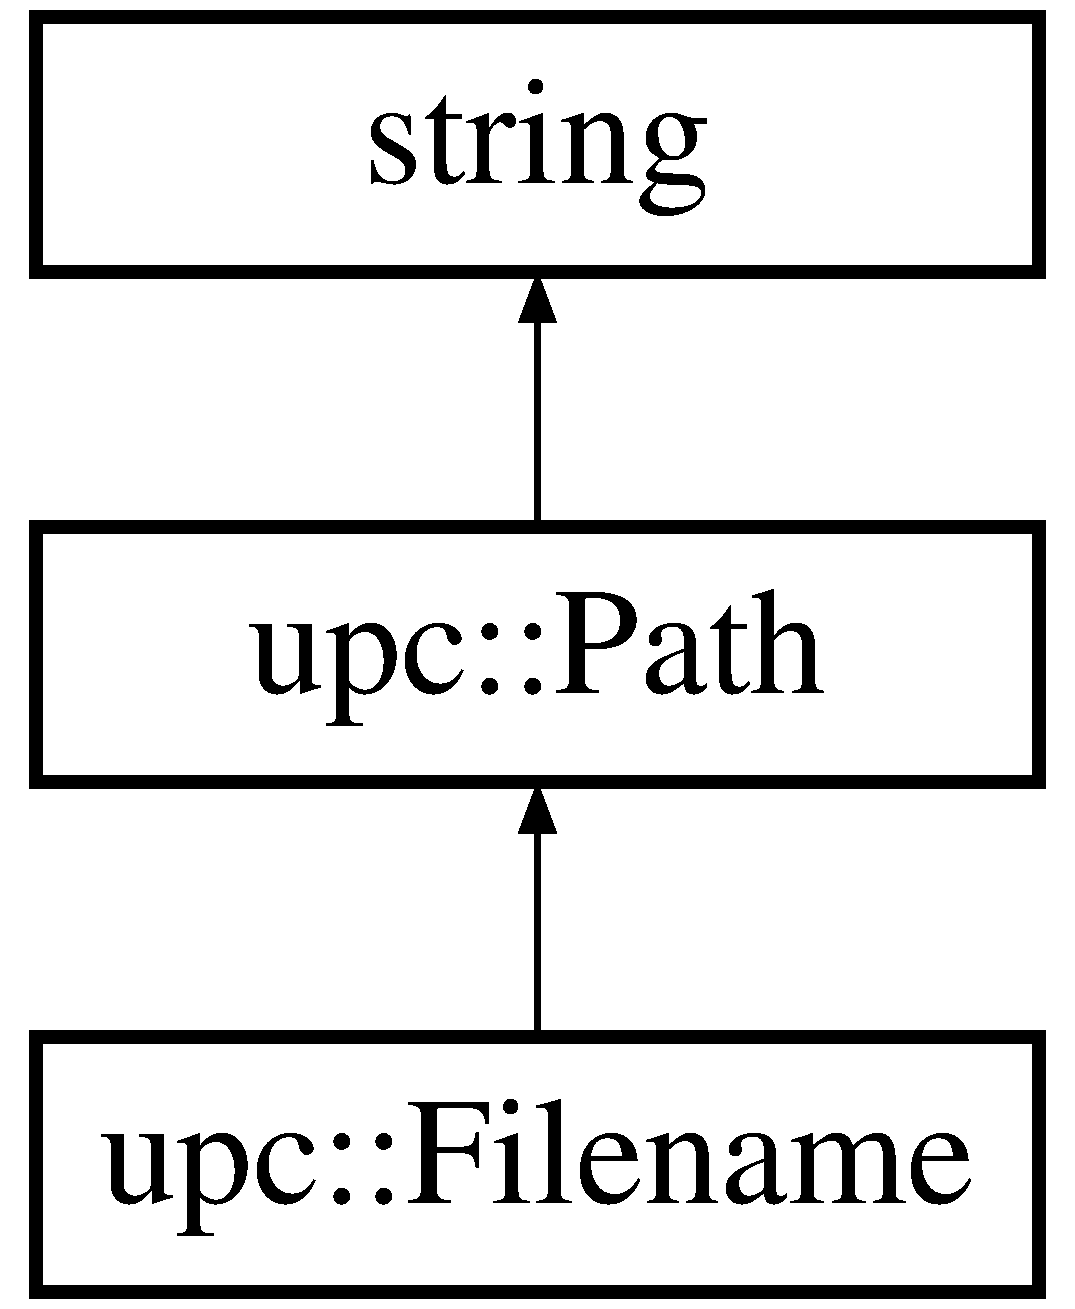
\includegraphics[height=3.000000cm]{classupc_1_1Filename}
\end{center}
\end{figure}
\subsection*{Public Member Functions}
\begin{DoxyCompactItemize}
\item 
\hyperlink{classupc_1_1Filename_ab3ba943521dc541e1eed8a3560d4c728}{Filename} ()
\item 
\hyperlink{classupc_1_1Filename_a80bdd15a0d0da8cf97a59125c3cae2c9}{Filename} (const \hyperlink{classupc_1_1Path}{Path} \&p)
\item 
\hyperlink{classupc_1_1Filename_a13e550c5b28bf991c84c053035760ed4}{Filename} (const string \&p)
\item 
\hyperlink{classupc_1_1Filename_a005b26738aa7db3b9f89258600b1e6f3}{Filename} (const char $\ast$p)
\item 
bool \hyperlink{classupc_1_1Filename_a5a53af16ef50db8e0f23ca9e96f6c1d0}{check\+Dir} (bool create=true) const 
\item 
bool \hyperlink{classupc_1_1Filename_af1ea3e760d5dc975dc404b81b3dd495d}{exist} () const 
\item 
\hyperlink{classupc_1_1Directory}{Directory} \hyperlink{classupc_1_1Filename_a5bef869d9bf781b7fbdc7e6e4de13558}{path} () const 
\item 
long long \hyperlink{classupc_1_1Filename_a232b2a742810eb8f213644cd367c8905}{size} () const 
\item 
virtual \hyperlink{classupc_1_1Filename_a873dadf99283f10286cb95cf4f951d1d}{$\sim$\+Filename} ()
\end{DoxyCompactItemize}


\subsection{Constructor \& Destructor Documentation}
\index{upc\+::\+Filename@{upc\+::\+Filename}!Filename@{Filename}}
\index{Filename@{Filename}!upc\+::\+Filename@{upc\+::\+Filename}}
\subsubsection[{\texorpdfstring{Filename()}{Filename()}}]{\setlength{\rightskip}{0pt plus 5cm}upc\+::\+Filename\+::\+Filename (
\begin{DoxyParamCaption}
{}
\end{DoxyParamCaption}
)\hspace{0.3cm}{\ttfamily [inline]}}\hypertarget{classupc_1_1Filename_ab3ba943521dc541e1eed8a3560d4c728}{}\label{classupc_1_1Filename_ab3ba943521dc541e1eed8a3560d4c728}
\index{upc\+::\+Filename@{upc\+::\+Filename}!Filename@{Filename}}
\index{Filename@{Filename}!upc\+::\+Filename@{upc\+::\+Filename}}
\subsubsection[{\texorpdfstring{Filename(const Path \&p)}{Filename(const Path &p)}}]{\setlength{\rightskip}{0pt plus 5cm}upc\+::\+Filename\+::\+Filename (
\begin{DoxyParamCaption}
\item[{const {\bf Path} \&}]{p}
\end{DoxyParamCaption}
)\hspace{0.3cm}{\ttfamily [inline]}}\hypertarget{classupc_1_1Filename_a80bdd15a0d0da8cf97a59125c3cae2c9}{}\label{classupc_1_1Filename_a80bdd15a0d0da8cf97a59125c3cae2c9}
\index{upc\+::\+Filename@{upc\+::\+Filename}!Filename@{Filename}}
\index{Filename@{Filename}!upc\+::\+Filename@{upc\+::\+Filename}}
\subsubsection[{\texorpdfstring{Filename(const string \&p)}{Filename(const string &p)}}]{\setlength{\rightskip}{0pt plus 5cm}upc\+::\+Filename\+::\+Filename (
\begin{DoxyParamCaption}
\item[{const string \&}]{p}
\end{DoxyParamCaption}
)\hspace{0.3cm}{\ttfamily [inline]}}\hypertarget{classupc_1_1Filename_a13e550c5b28bf991c84c053035760ed4}{}\label{classupc_1_1Filename_a13e550c5b28bf991c84c053035760ed4}
\index{upc\+::\+Filename@{upc\+::\+Filename}!Filename@{Filename}}
\index{Filename@{Filename}!upc\+::\+Filename@{upc\+::\+Filename}}
\subsubsection[{\texorpdfstring{Filename(const char $\ast$p)}{Filename(const char *p)}}]{\setlength{\rightskip}{0pt plus 5cm}upc\+::\+Filename\+::\+Filename (
\begin{DoxyParamCaption}
\item[{const char $\ast$}]{p}
\end{DoxyParamCaption}
)\hspace{0.3cm}{\ttfamily [inline]}}\hypertarget{classupc_1_1Filename_a005b26738aa7db3b9f89258600b1e6f3}{}\label{classupc_1_1Filename_a005b26738aa7db3b9f89258600b1e6f3}
\index{upc\+::\+Filename@{upc\+::\+Filename}!````~Filename@{$\sim$\+Filename}}
\index{````~Filename@{$\sim$\+Filename}!upc\+::\+Filename@{upc\+::\+Filename}}
\subsubsection[{\texorpdfstring{$\sim$\+Filename()}{~Filename()}}]{\setlength{\rightskip}{0pt plus 5cm}virtual upc\+::\+Filename\+::$\sim$\+Filename (
\begin{DoxyParamCaption}
{}
\end{DoxyParamCaption}
)\hspace{0.3cm}{\ttfamily [inline]}, {\ttfamily [virtual]}}\hypertarget{classupc_1_1Filename_a873dadf99283f10286cb95cf4f951d1d}{}\label{classupc_1_1Filename_a873dadf99283f10286cb95cf4f951d1d}


\subsection{Member Function Documentation}
\index{upc\+::\+Filename@{upc\+::\+Filename}!check\+Dir@{check\+Dir}}
\index{check\+Dir@{check\+Dir}!upc\+::\+Filename@{upc\+::\+Filename}}
\subsubsection[{\texorpdfstring{check\+Dir(bool create=true) const }{checkDir(bool create=true) const }}]{\setlength{\rightskip}{0pt plus 5cm}bool upc\+::\+Filename\+::check\+Dir (
\begin{DoxyParamCaption}
\item[{bool}]{create = {\ttfamily true}}
\end{DoxyParamCaption}
) const}\hypertarget{classupc_1_1Filename_a5a53af16ef50db8e0f23ca9e96f6c1d0}{}\label{classupc_1_1Filename_a5a53af16ef50db8e0f23ca9e96f6c1d0}
\index{upc\+::\+Filename@{upc\+::\+Filename}!exist@{exist}}
\index{exist@{exist}!upc\+::\+Filename@{upc\+::\+Filename}}
\subsubsection[{\texorpdfstring{exist() const }{exist() const }}]{\setlength{\rightskip}{0pt plus 5cm}bool upc\+::\+Filename\+::exist (
\begin{DoxyParamCaption}
{}
\end{DoxyParamCaption}
) const}\hypertarget{classupc_1_1Filename_af1ea3e760d5dc975dc404b81b3dd495d}{}\label{classupc_1_1Filename_af1ea3e760d5dc975dc404b81b3dd495d}
\index{upc\+::\+Filename@{upc\+::\+Filename}!path@{path}}
\index{path@{path}!upc\+::\+Filename@{upc\+::\+Filename}}
\subsubsection[{\texorpdfstring{path() const }{path() const }}]{\setlength{\rightskip}{0pt plus 5cm}{\bf Directory} upc\+::\+Filename\+::path (
\begin{DoxyParamCaption}
{}
\end{DoxyParamCaption}
) const}\hypertarget{classupc_1_1Filename_a5bef869d9bf781b7fbdc7e6e4de13558}{}\label{classupc_1_1Filename_a5bef869d9bf781b7fbdc7e6e4de13558}
\index{upc\+::\+Filename@{upc\+::\+Filename}!size@{size}}
\index{size@{size}!upc\+::\+Filename@{upc\+::\+Filename}}
\subsubsection[{\texorpdfstring{size() const }{size() const }}]{\setlength{\rightskip}{0pt plus 5cm}long long upc\+::\+Filename\+::size (
\begin{DoxyParamCaption}
{}
\end{DoxyParamCaption}
) const}\hypertarget{classupc_1_1Filename_a232b2a742810eb8f213644cd367c8905}{}\label{classupc_1_1Filename_a232b2a742810eb8f213644cd367c8905}


The documentation for this class was generated from the following files\+:\begin{DoxyCompactItemize}
\item 
include/\hyperlink{filename_8h}{filename.\+h}\item 
pav/\hyperlink{filename_8cpp}{filename.\+cpp}\end{DoxyCompactItemize}

\hypertarget{classupc_1_1KeyValue}{}\section{upc\+:\+:Key\+Value Class Reference}
\label{classupc_1_1KeyValue}\index{upc\+::\+Key\+Value@{upc\+::\+Key\+Value}}


{\ttfamily \#include $<$keyvalue.\+h$>$}

\subsection*{Public Member Functions}
\begin{DoxyCompactItemize}
\item 
\hyperlink{classupc_1_1KeyValue_a16e43218b2cdf234929ad76c6a28de51}{Key\+Value} (const std\+::string \&raw\+\_\+parameters=\char`\"{}\char`\"{})
\item 
void \hyperlink{classupc_1_1KeyValue_aff88fb11aa97cd85fa0b398e34ed763a}{set} (const std\+::string \&raw\+\_\+parameters)
\begin{DoxyCompactList}\small\item\em Initialize table from string, e.\+g. \char`\"{}city=\+Barcelona; year=2015\char`\"{}. \end{DoxyCompactList}\item 
const std\+::string \& \hyperlink{classupc_1_1KeyValue_a26cd081e33ed9d29937a266688f250eb}{operator()} (const std\+::string \&key) const 
\begin{DoxyCompactList}\small\item\em Give the value (as a string) of a given key. \end{DoxyCompactList}\item 
bool \hyperlink{classupc_1_1KeyValue_ab0e78c55886853b14ed0b0a12d54ffe8}{to\+\_\+float} (const std\+::string \&key, \hyperlink{FFTReal__readme_8txt_a0ea2fae2a8106200bf378b90eae003cf}{float} \&) const 
\begin{DoxyCompactList}\small\item\em Get the value as a float. \end{DoxyCompactList}\item 
bool \hyperlink{classupc_1_1KeyValue_aec285f4f4eb0eb6dda44c15138f4a3d9}{to\+\_\+int} (const std\+::string \&key, int \&) const 
\begin{DoxyCompactList}\small\item\em Get the value as an int. \end{DoxyCompactList}\item 
bool \hyperlink{classupc_1_1KeyValue_a8413af4543c0103f01a4bf2c7e480650}{to\+\_\+vector} (const std\+::string \&key, std\+::vector$<$ \hyperlink{FFTReal__readme_8txt_a0ea2fae2a8106200bf378b90eae003cf}{float} $>$ \&) const 
\begin{DoxyCompactList}\small\item\em Get the value as a vector of floats. \end{DoxyCompactList}\end{DoxyCompactItemize}
\subsection*{Private Types}
\begin{DoxyCompactItemize}
\item 
typedef std\+::map$<$ std\+::string, std\+::string $>$ \hyperlink{classupc_1_1KeyValue_a7f07bc656bce50d056f5ad0d118b2562}{S2\+S\+M\+AP}
\item 
typedef S2\+S\+M\+A\+P\+::iterator \hyperlink{classupc_1_1KeyValue_a3c6dedd86b7be8eadf7334b08d97364c}{iterator}
\item 
typedef S2\+S\+M\+A\+P\+::const\+\_\+iterator \hyperlink{classupc_1_1KeyValue_a1979eeaeda79e31e99fc6dc75b971373}{const\+\_\+iterator}
\end{DoxyCompactItemize}
\subsection*{Private Attributes}
\begin{DoxyCompactItemize}
\item 
\hyperlink{classupc_1_1KeyValue_a7f07bc656bce50d056f5ad0d118b2562}{S2\+S\+M\+AP} \hyperlink{classupc_1_1KeyValue_a5a75d6c2fb82f07ba0798cfeceefff01}{kv}
\begin{DoxyCompactList}\small\item\em Map to store key/value. \end{DoxyCompactList}\end{DoxyCompactItemize}


\subsection{Detailed Description}
Class to tranform parameters in a string format as a key/value table

string s = \char`\"{}\+A=3; B=hola; lista=3,2,5;\char`\"{} \hyperlink{classupc_1_1KeyValue}{Key\+Value} kv(s); cout $<$$<$ kv(\char`\"{}\+A\char`\"{}) $<$$<$ \textquotesingle{}~\newline
\textquotesingle{}; cout $<$$<$ kv(\char`\"{}\+B\char`\"{}) $<$$<$ \textquotesingle{}~\newline
\textquotesingle{}; cout $<$$<$ kv(\char`\"{}lista\char`\"{}) $<$$<$ \textquotesingle{}~\newline
\textquotesingle{};

This will show \char`\"{}3\char`\"{} \char`\"{}hola\char`\"{} \char`\"{}3,2,5\char`\"{}

Furthermore, it can transform the result to int, float, vector.

E.\+g.\+: int i; kv.\+to\+\_\+int(\char`\"{}\+A\char`\"{},i); vector$<$float$>$ x; kv.\+to\+\_\+vector(\char`\"{}lista\char`\"{}, x); 

\subsection{Member Typedef Documentation}
\index{upc\+::\+Key\+Value@{upc\+::\+Key\+Value}!const\+\_\+iterator@{const\+\_\+iterator}}
\index{const\+\_\+iterator@{const\+\_\+iterator}!upc\+::\+Key\+Value@{upc\+::\+Key\+Value}}
\subsubsection[{\texorpdfstring{const\+\_\+iterator}{const_iterator}}]{\setlength{\rightskip}{0pt plus 5cm}typedef S2\+S\+M\+A\+P\+::const\+\_\+iterator {\bf upc\+::\+Key\+Value\+::const\+\_\+iterator}\hspace{0.3cm}{\ttfamily [private]}}\hypertarget{classupc_1_1KeyValue_a1979eeaeda79e31e99fc6dc75b971373}{}\label{classupc_1_1KeyValue_a1979eeaeda79e31e99fc6dc75b971373}
\index{upc\+::\+Key\+Value@{upc\+::\+Key\+Value}!iterator@{iterator}}
\index{iterator@{iterator}!upc\+::\+Key\+Value@{upc\+::\+Key\+Value}}
\subsubsection[{\texorpdfstring{iterator}{iterator}}]{\setlength{\rightskip}{0pt plus 5cm}typedef S2\+S\+M\+A\+P\+::iterator {\bf upc\+::\+Key\+Value\+::iterator}\hspace{0.3cm}{\ttfamily [private]}}\hypertarget{classupc_1_1KeyValue_a3c6dedd86b7be8eadf7334b08d97364c}{}\label{classupc_1_1KeyValue_a3c6dedd86b7be8eadf7334b08d97364c}
\index{upc\+::\+Key\+Value@{upc\+::\+Key\+Value}!S2\+S\+M\+AP@{S2\+S\+M\+AP}}
\index{S2\+S\+M\+AP@{S2\+S\+M\+AP}!upc\+::\+Key\+Value@{upc\+::\+Key\+Value}}
\subsubsection[{\texorpdfstring{S2\+S\+M\+AP}{S2SMAP}}]{\setlength{\rightskip}{0pt plus 5cm}typedef std\+::map$<$std\+::string, std\+::string$>$ {\bf upc\+::\+Key\+Value\+::\+S2\+S\+M\+AP}\hspace{0.3cm}{\ttfamily [private]}}\hypertarget{classupc_1_1KeyValue_a7f07bc656bce50d056f5ad0d118b2562}{}\label{classupc_1_1KeyValue_a7f07bc656bce50d056f5ad0d118b2562}


\subsection{Constructor \& Destructor Documentation}
\index{upc\+::\+Key\+Value@{upc\+::\+Key\+Value}!Key\+Value@{Key\+Value}}
\index{Key\+Value@{Key\+Value}!upc\+::\+Key\+Value@{upc\+::\+Key\+Value}}
\subsubsection[{\texorpdfstring{Key\+Value(const std\+::string \&raw\+\_\+parameters="""")}{KeyValue(const std::string &raw_parameters="")}}]{\setlength{\rightskip}{0pt plus 5cm}Key\+Value\+::\+Key\+Value (
\begin{DoxyParamCaption}
\item[{const std\+::string \&}]{raw\+\_\+parameters = {\ttfamily \char`\"{}\char`\"{}}}
\end{DoxyParamCaption}
)}\hypertarget{classupc_1_1KeyValue_a16e43218b2cdf234929ad76c6a28de51}{}\label{classupc_1_1KeyValue_a16e43218b2cdf234929ad76c6a28de51}


\subsection{Member Function Documentation}
\index{upc\+::\+Key\+Value@{upc\+::\+Key\+Value}!operator()@{operator()}}
\index{operator()@{operator()}!upc\+::\+Key\+Value@{upc\+::\+Key\+Value}}
\subsubsection[{\texorpdfstring{operator()(const std\+::string \&key) const }{operator()(const std::string &key) const }}]{\setlength{\rightskip}{0pt plus 5cm}const std\+::string \& Key\+Value\+::operator() (
\begin{DoxyParamCaption}
\item[{const std\+::string \&}]{key}
\end{DoxyParamCaption}
) const}\hypertarget{classupc_1_1KeyValue_a26cd081e33ed9d29937a266688f250eb}{}\label{classupc_1_1KeyValue_a26cd081e33ed9d29937a266688f250eb}


Give the value (as a string) of a given key. 

\index{upc\+::\+Key\+Value@{upc\+::\+Key\+Value}!set@{set}}
\index{set@{set}!upc\+::\+Key\+Value@{upc\+::\+Key\+Value}}
\subsubsection[{\texorpdfstring{set(const std\+::string \&raw\+\_\+parameters)}{set(const std::string &raw_parameters)}}]{\setlength{\rightskip}{0pt plus 5cm}void Key\+Value\+::set (
\begin{DoxyParamCaption}
\item[{const std\+::string \&}]{raw\+\_\+parameters}
\end{DoxyParamCaption}
)}\hypertarget{classupc_1_1KeyValue_aff88fb11aa97cd85fa0b398e34ed763a}{}\label{classupc_1_1KeyValue_aff88fb11aa97cd85fa0b398e34ed763a}


Initialize table from string, e.\+g. \char`\"{}city=\+Barcelona; year=2015\char`\"{}. 

\index{upc\+::\+Key\+Value@{upc\+::\+Key\+Value}!to\+\_\+float@{to\+\_\+float}}
\index{to\+\_\+float@{to\+\_\+float}!upc\+::\+Key\+Value@{upc\+::\+Key\+Value}}
\subsubsection[{\texorpdfstring{to\+\_\+float(const std\+::string \&key, float \&) const }{to_float(const std::string &key, float &) const }}]{\setlength{\rightskip}{0pt plus 5cm}bool Key\+Value\+::to\+\_\+float (
\begin{DoxyParamCaption}
\item[{const std\+::string \&}]{key, }
\item[{{\bf float} \&}]{f}
\end{DoxyParamCaption}
) const}\hypertarget{classupc_1_1KeyValue_ab0e78c55886853b14ed0b0a12d54ffe8}{}\label{classupc_1_1KeyValue_ab0e78c55886853b14ed0b0a12d54ffe8}


Get the value as a float. 

\index{upc\+::\+Key\+Value@{upc\+::\+Key\+Value}!to\+\_\+int@{to\+\_\+int}}
\index{to\+\_\+int@{to\+\_\+int}!upc\+::\+Key\+Value@{upc\+::\+Key\+Value}}
\subsubsection[{\texorpdfstring{to\+\_\+int(const std\+::string \&key, int \&) const }{to_int(const std::string &key, int &) const }}]{\setlength{\rightskip}{0pt plus 5cm}bool Key\+Value\+::to\+\_\+int (
\begin{DoxyParamCaption}
\item[{const std\+::string \&}]{key, }
\item[{int \&}]{i}
\end{DoxyParamCaption}
) const}\hypertarget{classupc_1_1KeyValue_aec285f4f4eb0eb6dda44c15138f4a3d9}{}\label{classupc_1_1KeyValue_aec285f4f4eb0eb6dda44c15138f4a3d9}


Get the value as an int. 

\index{upc\+::\+Key\+Value@{upc\+::\+Key\+Value}!to\+\_\+vector@{to\+\_\+vector}}
\index{to\+\_\+vector@{to\+\_\+vector}!upc\+::\+Key\+Value@{upc\+::\+Key\+Value}}
\subsubsection[{\texorpdfstring{to\+\_\+vector(const std\+::string \&key, std\+::vector$<$ float $>$ \&) const }{to_vector(const std::string &key, std::vector< float > &) const }}]{\setlength{\rightskip}{0pt plus 5cm}bool Key\+Value\+::to\+\_\+vector (
\begin{DoxyParamCaption}
\item[{const std\+::string \&}]{key, }
\item[{std\+::vector$<$ {\bf float} $>$ \&}]{}
\end{DoxyParamCaption}
) const}\hypertarget{classupc_1_1KeyValue_a8413af4543c0103f01a4bf2c7e480650}{}\label{classupc_1_1KeyValue_a8413af4543c0103f01a4bf2c7e480650}


Get the value as a vector of floats. 



\subsection{Member Data Documentation}
\index{upc\+::\+Key\+Value@{upc\+::\+Key\+Value}!kv@{kv}}
\index{kv@{kv}!upc\+::\+Key\+Value@{upc\+::\+Key\+Value}}
\subsubsection[{\texorpdfstring{kv}{kv}}]{\setlength{\rightskip}{0pt plus 5cm}{\bf S2\+S\+M\+AP} upc\+::\+Key\+Value\+::kv\hspace{0.3cm}{\ttfamily [private]}}\hypertarget{classupc_1_1KeyValue_a5a75d6c2fb82f07ba0798cfeceefff01}{}\label{classupc_1_1KeyValue_a5a75d6c2fb82f07ba0798cfeceefff01}


Map to store key/value. 



The documentation for this class was generated from the following files\+:\begin{DoxyCompactItemize}
\item 
include/\hyperlink{keyvalue_8h}{keyvalue.\+h}\item 
pav/\hyperlink{keyvalue_8cpp}{keyvalue.\+cpp}\end{DoxyCompactItemize}

\hypertarget{classupc_1_1matrix}{}\section{upc\+:\+:matrix$<$ \+\_\+\+Ty $>$ Class Template Reference}
\label{classupc_1_1matrix}\index{upc\+::matrix$<$ \+\_\+\+Ty $>$@{upc\+::matrix$<$ \+\_\+\+Ty $>$}}


{\ttfamily \#include $<$matrix.\+h$>$}

\subsection*{Public Types}
\begin{DoxyCompactItemize}
\item 
typedef \hyperlink{classupc_1_1array_a85501f086a20ed6686ef78a242b2f302}{Tvector\+::size\+\_\+type} \hyperlink{classupc_1_1matrix_a0f2b47f0fc08216f8e0ef1cc1c022663}{size\+\_\+type}
\end{DoxyCompactItemize}
\subsection*{Public Member Functions}
\begin{DoxyCompactItemize}
\item 
\hyperlink{classupc_1_1matrix_a908e2ae559167d0376d2b095116029ab}{matrix} (\hyperlink{classupc_1_1matrix_a0f2b47f0fc08216f8e0ef1cc1c022663}{size\+\_\+type} \hyperlink{classupc_1_1matrix_a7b922be25c0cf0d255252a4fe7350ea2}{nrow}=0, \hyperlink{classupc_1_1matrix_a0f2b47f0fc08216f8e0ef1cc1c022663}{size\+\_\+type} \hyperlink{classupc_1_1matrix_a0e8f41d88948610215db9cc8eafa02a6}{ncol}=0)
\item 
\hyperlink{classupc_1_1matrix_aedb3ba241346dfac0655cf4b63715e7f}{matrix} (const \hyperlink{classupc_1_1matrix_a9e671131fc3af250bb4bad539474da9c}{\+\_\+\+Myt} \&o)
\item 
\hyperlink{classupc_1_1matrix_a0f2b47f0fc08216f8e0ef1cc1c022663}{size\+\_\+type} \hyperlink{classupc_1_1matrix_a7b922be25c0cf0d255252a4fe7350ea2}{nrow} () const 
\item 
\hyperlink{classupc_1_1matrix_a0f2b47f0fc08216f8e0ef1cc1c022663}{size\+\_\+type} \hyperlink{classupc_1_1matrix_a0e8f41d88948610215db9cc8eafa02a6}{ncol} () const 
\item 
\hyperlink{classupc_1_1matrix_af4880980335adaf4abe61988558472f5}{\+\_\+\+Ctptr} \hyperlink{classupc_1_1matrix_a773213642b2ba0beda6e19618e2b949a}{operator\mbox{[}$\,$\mbox{]}} (int i) const 
\item 
\hyperlink{classupc_1_1matrix_a75a85786a5de55cdfcdf1f205df1f3e8}{\+\_\+\+Tptr} \hyperlink{classupc_1_1matrix_a1016950fd091e3798fa475b5f2e90719}{operator\mbox{[}$\,$\mbox{]}} (int i)
\item 
const \hyperlink{classupc_1_1matrix_af4880980335adaf4abe61988558472f5}{\+\_\+\+Ctptr} $\ast$ \hyperlink{classupc_1_1matrix_add034dcb2c5abd3d6a728da60f5590e9}{m} () const 
\item 
\hyperlink{classupc_1_1matrix_a75a85786a5de55cdfcdf1f205df1f3e8}{\+\_\+\+Tptr} $\ast$ \hyperlink{classupc_1_1matrix_a6b505e71e56088332a4203f6b6032dcf}{m} ()
\item 
void \hyperlink{classupc_1_1matrix_aec394dcccbfaad5c75a013874814c475}{reset} ()
\item 
void \hyperlink{classupc_1_1matrix_ad9c957658ec403494af0d92fa2c499fb}{resize} (\hyperlink{classupc_1_1matrix_a0f2b47f0fc08216f8e0ef1cc1c022663}{size\+\_\+type} \hyperlink{classupc_1_1matrix_a7b922be25c0cf0d255252a4fe7350ea2}{nrow}, \hyperlink{classupc_1_1matrix_a0f2b47f0fc08216f8e0ef1cc1c022663}{size\+\_\+type} \hyperlink{classupc_1_1matrix_a0e8f41d88948610215db9cc8eafa02a6}{ncol})
\item 
\hyperlink{classupc_1_1matrix_a9e671131fc3af250bb4bad539474da9c}{\+\_\+\+Myt} \& \hyperlink{classupc_1_1matrix_a9a0d300fcfe6652fde1347c139291919}{operator=} (const \hyperlink{classupc_1_1matrix_a9e671131fc3af250bb4bad539474da9c}{\+\_\+\+Myt} \&other)
\end{DoxyCompactItemize}
\subsection*{Private Types}
\begin{DoxyCompactItemize}
\item 
typedef \hyperlink{classupc_1_1matrix}{matrix}$<$ \+\_\+\+Ty $>$ \hyperlink{classupc_1_1matrix_a9e671131fc3af250bb4bad539474da9c}{\+\_\+\+Myt}
\item 
typedef \hyperlink{classupc_1_1array}{array}$<$ \+\_\+\+Ty $>$ \hyperlink{classupc_1_1matrix_acebf527a1d5f301a17e38e08d5cea335}{Tvector}
\item 
typedef \hyperlink{classupc_1_1array_a420718228a4d845721303a19755f0d42}{Tvector\+::\+\_\+\+Ctptr} \hyperlink{classupc_1_1matrix_af4880980335adaf4abe61988558472f5}{\+\_\+\+Ctptr}
\item 
typedef \hyperlink{classupc_1_1array_a4ef66945898a2c393cff5be41de077d2}{Tvector\+::\+\_\+\+Tptr} \hyperlink{classupc_1_1matrix_a75a85786a5de55cdfcdf1f205df1f3e8}{\+\_\+\+Tptr}
\item 
typedef \hyperlink{classupc_1_1array}{array}$<$ \hyperlink{classupc_1_1matrix_a75a85786a5de55cdfcdf1f205df1f3e8}{\+\_\+\+Tptr} $>$ \hyperlink{classupc_1_1matrix_a1f8337796d73b88280f6a517d2d1f20d}{Pvector}
\end{DoxyCompactItemize}
\subsection*{Private Attributes}
\begin{DoxyCompactItemize}
\item 
\hyperlink{classupc_1_1matrix_acebf527a1d5f301a17e38e08d5cea335}{Tvector} \hyperlink{classupc_1_1matrix_a1fd23b090b8e985c526d913792ad0f96}{m\+\_\+v}
\item 
\hyperlink{classupc_1_1matrix_a1f8337796d73b88280f6a517d2d1f20d}{Pvector} \hyperlink{classupc_1_1matrix_a01c5df069e0cddf9efcb5632a7e9c220}{m\+\_\+p}
\item 
\hyperlink{classupc_1_1matrix_a0f2b47f0fc08216f8e0ef1cc1c022663}{size\+\_\+type} \hyperlink{classupc_1_1matrix_a2a32ddd89dd5b9c85d95498f9fb77c70}{m\+\_\+nrow}
\item 
\hyperlink{classupc_1_1matrix_a0f2b47f0fc08216f8e0ef1cc1c022663}{size\+\_\+type} \hyperlink{classupc_1_1matrix_a053950016358b76da92c0a25c01987e9}{m\+\_\+ncol}
\end{DoxyCompactItemize}


\subsection{Member Typedef Documentation}
\index{upc\+::matrix@{upc\+::matrix}!\+\_\+\+Ctptr@{\+\_\+\+Ctptr}}
\index{\+\_\+\+Ctptr@{\+\_\+\+Ctptr}!upc\+::matrix@{upc\+::matrix}}
\subsubsection[{\texorpdfstring{\+\_\+\+Ctptr}{_Ctptr}}]{\setlength{\rightskip}{0pt plus 5cm}template$<$class \+\_\+\+Ty$>$ typedef {\bf Tvector\+::\+\_\+\+Ctptr} {\bf upc\+::matrix}$<$ \+\_\+\+Ty $>$\+::{\bf \+\_\+\+Ctptr}\hspace{0.3cm}{\ttfamily [private]}}\hypertarget{classupc_1_1matrix_af4880980335adaf4abe61988558472f5}{}\label{classupc_1_1matrix_af4880980335adaf4abe61988558472f5}
\index{upc\+::matrix@{upc\+::matrix}!\+\_\+\+Myt@{\+\_\+\+Myt}}
\index{\+\_\+\+Myt@{\+\_\+\+Myt}!upc\+::matrix@{upc\+::matrix}}
\subsubsection[{\texorpdfstring{\+\_\+\+Myt}{_Myt}}]{\setlength{\rightskip}{0pt plus 5cm}template$<$class \+\_\+\+Ty$>$ typedef {\bf matrix}$<$\+\_\+\+Ty$>$ {\bf upc\+::matrix}$<$ \+\_\+\+Ty $>$\+::{\bf \+\_\+\+Myt}\hspace{0.3cm}{\ttfamily [private]}}\hypertarget{classupc_1_1matrix_a9e671131fc3af250bb4bad539474da9c}{}\label{classupc_1_1matrix_a9e671131fc3af250bb4bad539474da9c}
\index{upc\+::matrix@{upc\+::matrix}!\+\_\+\+Tptr@{\+\_\+\+Tptr}}
\index{\+\_\+\+Tptr@{\+\_\+\+Tptr}!upc\+::matrix@{upc\+::matrix}}
\subsubsection[{\texorpdfstring{\+\_\+\+Tptr}{_Tptr}}]{\setlength{\rightskip}{0pt plus 5cm}template$<$class \+\_\+\+Ty$>$ typedef {\bf Tvector\+::\+\_\+\+Tptr} {\bf upc\+::matrix}$<$ \+\_\+\+Ty $>$\+::{\bf \+\_\+\+Tptr}\hspace{0.3cm}{\ttfamily [private]}}\hypertarget{classupc_1_1matrix_a75a85786a5de55cdfcdf1f205df1f3e8}{}\label{classupc_1_1matrix_a75a85786a5de55cdfcdf1f205df1f3e8}
\index{upc\+::matrix@{upc\+::matrix}!Pvector@{Pvector}}
\index{Pvector@{Pvector}!upc\+::matrix@{upc\+::matrix}}
\subsubsection[{\texorpdfstring{Pvector}{Pvector}}]{\setlength{\rightskip}{0pt plus 5cm}template$<$class \+\_\+\+Ty$>$ typedef {\bf array}$<${\bf \+\_\+\+Tptr}$>$ {\bf upc\+::matrix}$<$ \+\_\+\+Ty $>$\+::{\bf Pvector}\hspace{0.3cm}{\ttfamily [private]}}\hypertarget{classupc_1_1matrix_a1f8337796d73b88280f6a517d2d1f20d}{}\label{classupc_1_1matrix_a1f8337796d73b88280f6a517d2d1f20d}
\index{upc\+::matrix@{upc\+::matrix}!size\+\_\+type@{size\+\_\+type}}
\index{size\+\_\+type@{size\+\_\+type}!upc\+::matrix@{upc\+::matrix}}
\subsubsection[{\texorpdfstring{size\+\_\+type}{size_type}}]{\setlength{\rightskip}{0pt plus 5cm}template$<$class \+\_\+\+Ty$>$ typedef {\bf Tvector\+::size\+\_\+type} {\bf upc\+::matrix}$<$ \+\_\+\+Ty $>$\+::{\bf size\+\_\+type}}\hypertarget{classupc_1_1matrix_a0f2b47f0fc08216f8e0ef1cc1c022663}{}\label{classupc_1_1matrix_a0f2b47f0fc08216f8e0ef1cc1c022663}
\index{upc\+::matrix@{upc\+::matrix}!Tvector@{Tvector}}
\index{Tvector@{Tvector}!upc\+::matrix@{upc\+::matrix}}
\subsubsection[{\texorpdfstring{Tvector}{Tvector}}]{\setlength{\rightskip}{0pt plus 5cm}template$<$class \+\_\+\+Ty$>$ typedef {\bf array}$<$\+\_\+\+Ty$>$ {\bf upc\+::matrix}$<$ \+\_\+\+Ty $>$\+::{\bf Tvector}\hspace{0.3cm}{\ttfamily [private]}}\hypertarget{classupc_1_1matrix_acebf527a1d5f301a17e38e08d5cea335}{}\label{classupc_1_1matrix_acebf527a1d5f301a17e38e08d5cea335}


\subsection{Constructor \& Destructor Documentation}
\index{upc\+::matrix@{upc\+::matrix}!matrix@{matrix}}
\index{matrix@{matrix}!upc\+::matrix@{upc\+::matrix}}
\subsubsection[{\texorpdfstring{matrix(size\+\_\+type nrow=0, size\+\_\+type ncol=0)}{matrix(size_type nrow=0, size_type ncol=0)}}]{\setlength{\rightskip}{0pt plus 5cm}template$<$class \+\_\+\+Ty$>$ {\bf upc\+::matrix}$<$ \+\_\+\+Ty $>$\+::{\bf matrix} (
\begin{DoxyParamCaption}
\item[{{\bf size\+\_\+type}}]{nrow = {\ttfamily 0}, }
\item[{{\bf size\+\_\+type}}]{ncol = {\ttfamily 0}}
\end{DoxyParamCaption}
)\hspace{0.3cm}{\ttfamily [inline]}, {\ttfamily [explicit]}}\hypertarget{classupc_1_1matrix_a908e2ae559167d0376d2b095116029ab}{}\label{classupc_1_1matrix_a908e2ae559167d0376d2b095116029ab}
\index{upc\+::matrix@{upc\+::matrix}!matrix@{matrix}}
\index{matrix@{matrix}!upc\+::matrix@{upc\+::matrix}}
\subsubsection[{\texorpdfstring{matrix(const \+\_\+\+Myt \&o)}{matrix(const _Myt &o)}}]{\setlength{\rightskip}{0pt plus 5cm}template$<$class \+\_\+\+Ty$>$ {\bf upc\+::matrix}$<$ \+\_\+\+Ty $>$\+::{\bf matrix} (
\begin{DoxyParamCaption}
\item[{const {\bf \+\_\+\+Myt} \&}]{o}
\end{DoxyParamCaption}
)\hspace{0.3cm}{\ttfamily [inline]}}\hypertarget{classupc_1_1matrix_aedb3ba241346dfac0655cf4b63715e7f}{}\label{classupc_1_1matrix_aedb3ba241346dfac0655cf4b63715e7f}


\subsection{Member Function Documentation}
\index{upc\+::matrix@{upc\+::matrix}!m@{m}}
\index{m@{m}!upc\+::matrix@{upc\+::matrix}}
\subsubsection[{\texorpdfstring{m() const }{m() const }}]{\setlength{\rightskip}{0pt plus 5cm}template$<$class \+\_\+\+Ty$>$ const {\bf \+\_\+\+Ctptr}$\ast$ {\bf upc\+::matrix}$<$ \+\_\+\+Ty $>$\+::m (
\begin{DoxyParamCaption}
{}
\end{DoxyParamCaption}
) const\hspace{0.3cm}{\ttfamily [inline]}}\hypertarget{classupc_1_1matrix_add034dcb2c5abd3d6a728da60f5590e9}{}\label{classupc_1_1matrix_add034dcb2c5abd3d6a728da60f5590e9}
\index{upc\+::matrix@{upc\+::matrix}!m@{m}}
\index{m@{m}!upc\+::matrix@{upc\+::matrix}}
\subsubsection[{\texorpdfstring{m()}{m()}}]{\setlength{\rightskip}{0pt plus 5cm}template$<$class \+\_\+\+Ty$>$ {\bf \+\_\+\+Tptr}$\ast$ {\bf upc\+::matrix}$<$ \+\_\+\+Ty $>$\+::m (
\begin{DoxyParamCaption}
{}
\end{DoxyParamCaption}
)\hspace{0.3cm}{\ttfamily [inline]}}\hypertarget{classupc_1_1matrix_a6b505e71e56088332a4203f6b6032dcf}{}\label{classupc_1_1matrix_a6b505e71e56088332a4203f6b6032dcf}
\index{upc\+::matrix@{upc\+::matrix}!ncol@{ncol}}
\index{ncol@{ncol}!upc\+::matrix@{upc\+::matrix}}
\subsubsection[{\texorpdfstring{ncol() const }{ncol() const }}]{\setlength{\rightskip}{0pt plus 5cm}template$<$class \+\_\+\+Ty$>$ {\bf size\+\_\+type} {\bf upc\+::matrix}$<$ \+\_\+\+Ty $>$\+::ncol (
\begin{DoxyParamCaption}
{}
\end{DoxyParamCaption}
) const\hspace{0.3cm}{\ttfamily [inline]}}\hypertarget{classupc_1_1matrix_a0e8f41d88948610215db9cc8eafa02a6}{}\label{classupc_1_1matrix_a0e8f41d88948610215db9cc8eafa02a6}
\index{upc\+::matrix@{upc\+::matrix}!nrow@{nrow}}
\index{nrow@{nrow}!upc\+::matrix@{upc\+::matrix}}
\subsubsection[{\texorpdfstring{nrow() const }{nrow() const }}]{\setlength{\rightskip}{0pt plus 5cm}template$<$class \+\_\+\+Ty$>$ {\bf size\+\_\+type} {\bf upc\+::matrix}$<$ \+\_\+\+Ty $>$\+::nrow (
\begin{DoxyParamCaption}
{}
\end{DoxyParamCaption}
) const\hspace{0.3cm}{\ttfamily [inline]}}\hypertarget{classupc_1_1matrix_a7b922be25c0cf0d255252a4fe7350ea2}{}\label{classupc_1_1matrix_a7b922be25c0cf0d255252a4fe7350ea2}
\index{upc\+::matrix@{upc\+::matrix}!operator=@{operator=}}
\index{operator=@{operator=}!upc\+::matrix@{upc\+::matrix}}
\subsubsection[{\texorpdfstring{operator=(const \+\_\+\+Myt \&other)}{operator=(const _Myt &other)}}]{\setlength{\rightskip}{0pt plus 5cm}template$<$class \+\_\+\+Ty$>$ {\bf \+\_\+\+Myt}\& {\bf upc\+::matrix}$<$ \+\_\+\+Ty $>$\+::operator= (
\begin{DoxyParamCaption}
\item[{const {\bf \+\_\+\+Myt} \&}]{other}
\end{DoxyParamCaption}
)\hspace{0.3cm}{\ttfamily [inline]}}\hypertarget{classupc_1_1matrix_a9a0d300fcfe6652fde1347c139291919}{}\label{classupc_1_1matrix_a9a0d300fcfe6652fde1347c139291919}
\index{upc\+::matrix@{upc\+::matrix}!operator\mbox{[}$\,$\mbox{]}@{operator[]}}
\index{operator\mbox{[}$\,$\mbox{]}@{operator[]}!upc\+::matrix@{upc\+::matrix}}
\subsubsection[{\texorpdfstring{operator[](int i) const }{operator[](int i) const }}]{\setlength{\rightskip}{0pt plus 5cm}template$<$class \+\_\+\+Ty$>$ {\bf \+\_\+\+Ctptr} {\bf upc\+::matrix}$<$ \+\_\+\+Ty $>$\+::operator\mbox{[}$\,$\mbox{]} (
\begin{DoxyParamCaption}
\item[{int}]{i}
\end{DoxyParamCaption}
) const\hspace{0.3cm}{\ttfamily [inline]}}\hypertarget{classupc_1_1matrix_a773213642b2ba0beda6e19618e2b949a}{}\label{classupc_1_1matrix_a773213642b2ba0beda6e19618e2b949a}
\index{upc\+::matrix@{upc\+::matrix}!operator\mbox{[}$\,$\mbox{]}@{operator[]}}
\index{operator\mbox{[}$\,$\mbox{]}@{operator[]}!upc\+::matrix@{upc\+::matrix}}
\subsubsection[{\texorpdfstring{operator[](int i)}{operator[](int i)}}]{\setlength{\rightskip}{0pt plus 5cm}template$<$class \+\_\+\+Ty$>$ {\bf \+\_\+\+Tptr} {\bf upc\+::matrix}$<$ \+\_\+\+Ty $>$\+::operator\mbox{[}$\,$\mbox{]} (
\begin{DoxyParamCaption}
\item[{int}]{i}
\end{DoxyParamCaption}
)\hspace{0.3cm}{\ttfamily [inline]}}\hypertarget{classupc_1_1matrix_a1016950fd091e3798fa475b5f2e90719}{}\label{classupc_1_1matrix_a1016950fd091e3798fa475b5f2e90719}
\index{upc\+::matrix@{upc\+::matrix}!reset@{reset}}
\index{reset@{reset}!upc\+::matrix@{upc\+::matrix}}
\subsubsection[{\texorpdfstring{reset()}{reset()}}]{\setlength{\rightskip}{0pt plus 5cm}template$<$class \+\_\+\+Ty$>$ void {\bf upc\+::matrix}$<$ \+\_\+\+Ty $>$\+::reset (
\begin{DoxyParamCaption}
{}
\end{DoxyParamCaption}
)\hspace{0.3cm}{\ttfamily [inline]}}\hypertarget{classupc_1_1matrix_aec394dcccbfaad5c75a013874814c475}{}\label{classupc_1_1matrix_aec394dcccbfaad5c75a013874814c475}
\index{upc\+::matrix@{upc\+::matrix}!resize@{resize}}
\index{resize@{resize}!upc\+::matrix@{upc\+::matrix}}
\subsubsection[{\texorpdfstring{resize(size\+\_\+type nrow, size\+\_\+type ncol)}{resize(size_type nrow, size_type ncol)}}]{\setlength{\rightskip}{0pt plus 5cm}template$<$class \+\_\+\+Ty$>$ void {\bf upc\+::matrix}$<$ \+\_\+\+Ty $>$\+::resize (
\begin{DoxyParamCaption}
\item[{{\bf size\+\_\+type}}]{nrow, }
\item[{{\bf size\+\_\+type}}]{ncol}
\end{DoxyParamCaption}
)\hspace{0.3cm}{\ttfamily [inline]}}\hypertarget{classupc_1_1matrix_ad9c957658ec403494af0d92fa2c499fb}{}\label{classupc_1_1matrix_ad9c957658ec403494af0d92fa2c499fb}


\subsection{Member Data Documentation}
\index{upc\+::matrix@{upc\+::matrix}!m\+\_\+ncol@{m\+\_\+ncol}}
\index{m\+\_\+ncol@{m\+\_\+ncol}!upc\+::matrix@{upc\+::matrix}}
\subsubsection[{\texorpdfstring{m\+\_\+ncol}{m_ncol}}]{\setlength{\rightskip}{0pt plus 5cm}template$<$class \+\_\+\+Ty$>$ {\bf size\+\_\+type} {\bf upc\+::matrix}$<$ \+\_\+\+Ty $>$\+::m\+\_\+ncol\hspace{0.3cm}{\ttfamily [private]}}\hypertarget{classupc_1_1matrix_a053950016358b76da92c0a25c01987e9}{}\label{classupc_1_1matrix_a053950016358b76da92c0a25c01987e9}
\index{upc\+::matrix@{upc\+::matrix}!m\+\_\+nrow@{m\+\_\+nrow}}
\index{m\+\_\+nrow@{m\+\_\+nrow}!upc\+::matrix@{upc\+::matrix}}
\subsubsection[{\texorpdfstring{m\+\_\+nrow}{m_nrow}}]{\setlength{\rightskip}{0pt plus 5cm}template$<$class \+\_\+\+Ty$>$ {\bf size\+\_\+type} {\bf upc\+::matrix}$<$ \+\_\+\+Ty $>$\+::m\+\_\+nrow\hspace{0.3cm}{\ttfamily [private]}}\hypertarget{classupc_1_1matrix_a2a32ddd89dd5b9c85d95498f9fb77c70}{}\label{classupc_1_1matrix_a2a32ddd89dd5b9c85d95498f9fb77c70}
\index{upc\+::matrix@{upc\+::matrix}!m\+\_\+p@{m\+\_\+p}}
\index{m\+\_\+p@{m\+\_\+p}!upc\+::matrix@{upc\+::matrix}}
\subsubsection[{\texorpdfstring{m\+\_\+p}{m_p}}]{\setlength{\rightskip}{0pt plus 5cm}template$<$class \+\_\+\+Ty$>$ {\bf Pvector} {\bf upc\+::matrix}$<$ \+\_\+\+Ty $>$\+::m\+\_\+p\hspace{0.3cm}{\ttfamily [private]}}\hypertarget{classupc_1_1matrix_a01c5df069e0cddf9efcb5632a7e9c220}{}\label{classupc_1_1matrix_a01c5df069e0cddf9efcb5632a7e9c220}
\index{upc\+::matrix@{upc\+::matrix}!m\+\_\+v@{m\+\_\+v}}
\index{m\+\_\+v@{m\+\_\+v}!upc\+::matrix@{upc\+::matrix}}
\subsubsection[{\texorpdfstring{m\+\_\+v}{m_v}}]{\setlength{\rightskip}{0pt plus 5cm}template$<$class \+\_\+\+Ty$>$ {\bf Tvector} {\bf upc\+::matrix}$<$ \+\_\+\+Ty $>$\+::m\+\_\+v\hspace{0.3cm}{\ttfamily [private]}}\hypertarget{classupc_1_1matrix_a1fd23b090b8e985c526d913792ad0f96}{}\label{classupc_1_1matrix_a1fd23b090b8e985c526d913792ad0f96}


The documentation for this class was generated from the following file\+:\begin{DoxyCompactItemize}
\item 
include/\hyperlink{matrix_8h}{matrix.\+h}\end{DoxyCompactItemize}

\hypertarget{classffft_1_1OscSinCos}{}\section{ffft\+:\+:Osc\+Sin\+Cos$<$ T $>$ Class Template Reference}
\label{classffft_1_1OscSinCos}\index{ffft\+::\+Osc\+Sin\+Cos$<$ T $>$@{ffft\+::\+Osc\+Sin\+Cos$<$ T $>$}}


{\ttfamily \#include $<$Osc\+Sin\+Cos.\+h$>$}

\subsection*{Public Types}
\begin{DoxyCompactItemize}
\item 
typedef T \hyperlink{classffft_1_1OscSinCos_af91237051e92ce0af7aaf38b1826244d}{Data\+Type}
\end{DoxyCompactItemize}
\subsection*{Public Member Functions}
\begin{DoxyCompactItemize}
\item 
\hyperlink{classffft_1_1OscSinCos_aed332791021f51d86b05594629244f1e}{Osc\+Sin\+Cos} ()
\item 
\hyperlink{def_8h_a31b2ada863c9efa7455efae4e13661f3}{ffft\+\_\+\+F\+O\+R\+C\+E\+I\+N\+L\+I\+NE} void \hyperlink{classffft_1_1OscSinCos_ad41139a76b16a5af136d1e730a9143dc}{set\+\_\+step} (double angle\+\_\+rad)
\item 
\hyperlink{def_8h_a31b2ada863c9efa7455efae4e13661f3}{ffft\+\_\+\+F\+O\+R\+C\+E\+I\+N\+L\+I\+NE} \hyperlink{classffft_1_1OscSinCos_af91237051e92ce0af7aaf38b1826244d}{Data\+Type} \hyperlink{classffft_1_1OscSinCos_aa903b64bed3d46a27aeb5af7d7154eb3}{get\+\_\+cos} () const 
\item 
\hyperlink{def_8h_a31b2ada863c9efa7455efae4e13661f3}{ffft\+\_\+\+F\+O\+R\+C\+E\+I\+N\+L\+I\+NE} \hyperlink{classffft_1_1OscSinCos_af91237051e92ce0af7aaf38b1826244d}{Data\+Type} \hyperlink{classffft_1_1OscSinCos_a3e336802d9e10288483d477bfdf50c20}{get\+\_\+sin} () const 
\item 
\hyperlink{def_8h_a31b2ada863c9efa7455efae4e13661f3}{ffft\+\_\+\+F\+O\+R\+C\+E\+I\+N\+L\+I\+NE} void \hyperlink{classffft_1_1OscSinCos_a442975ce6388271ea78998c080364e08}{step} ()
\item 
\hyperlink{def_8h_a31b2ada863c9efa7455efae4e13661f3}{ffft\+\_\+\+F\+O\+R\+C\+E\+I\+N\+L\+I\+NE} void \hyperlink{classffft_1_1OscSinCos_a1be4a9ec10517ae2615d2925c05d7d29}{clear\+\_\+buffers} ()
\end{DoxyCompactItemize}
\subsection*{Private Member Functions}
\begin{DoxyCompactItemize}
\item 
\hyperlink{classffft_1_1OscSinCos_a55142abe630264728cdec4eac8cdc932}{Osc\+Sin\+Cos} (const \hyperlink{classffft_1_1OscSinCos}{Osc\+Sin\+Cos} \&other)
\item 
\hyperlink{classffft_1_1OscSinCos}{Osc\+Sin\+Cos} \& \hyperlink{classffft_1_1OscSinCos_aa1205e8382acd3b8ccfc5bd4dc1a6ac6}{operator=} (const \hyperlink{classffft_1_1OscSinCos}{Osc\+Sin\+Cos} \&other)
\item 
bool \hyperlink{classffft_1_1OscSinCos_a77055dcda40cc256ec6f481fe9779bee}{operator==} (const \hyperlink{classffft_1_1OscSinCos}{Osc\+Sin\+Cos} \&other)
\item 
bool \hyperlink{classffft_1_1OscSinCos_a39334cbb48e55afe3db6a3d36069f052}{operator!=} (const \hyperlink{classffft_1_1OscSinCos}{Osc\+Sin\+Cos} \&other)
\end{DoxyCompactItemize}
\subsection*{Private Attributes}
\begin{DoxyCompactItemize}
\item 
\hyperlink{classffft_1_1OscSinCos_af91237051e92ce0af7aaf38b1826244d}{Data\+Type} \hyperlink{classffft_1_1OscSinCos_a27b849cf4cd82b159f969c9de39197d5}{\+\_\+pos\+\_\+cos}
\item 
\hyperlink{classffft_1_1OscSinCos_af91237051e92ce0af7aaf38b1826244d}{Data\+Type} \hyperlink{classffft_1_1OscSinCos_afddb969706b1b473229bf433d308b670}{\+\_\+pos\+\_\+sin}
\item 
\hyperlink{classffft_1_1OscSinCos_af91237051e92ce0af7aaf38b1826244d}{Data\+Type} \hyperlink{classffft_1_1OscSinCos_ad0bdc750147d730559311933ac124ab2}{\+\_\+step\+\_\+cos}
\item 
\hyperlink{classffft_1_1OscSinCos_af91237051e92ce0af7aaf38b1826244d}{Data\+Type} \hyperlink{classffft_1_1OscSinCos_a1a55c352898b66ee77bff85e116fdce0}{\+\_\+step\+\_\+sin}
\end{DoxyCompactItemize}


\subsection{Member Typedef Documentation}
\index{ffft\+::\+Osc\+Sin\+Cos@{ffft\+::\+Osc\+Sin\+Cos}!Data\+Type@{Data\+Type}}
\index{Data\+Type@{Data\+Type}!ffft\+::\+Osc\+Sin\+Cos@{ffft\+::\+Osc\+Sin\+Cos}}
\subsubsection[{\texorpdfstring{Data\+Type}{DataType}}]{\setlength{\rightskip}{0pt plus 5cm}template$<$class T$>$ typedef T {\bf ffft\+::\+Osc\+Sin\+Cos}$<$ T $>$\+::{\bf Data\+Type}}\hypertarget{classffft_1_1OscSinCos_af91237051e92ce0af7aaf38b1826244d}{}\label{classffft_1_1OscSinCos_af91237051e92ce0af7aaf38b1826244d}


\subsection{Constructor \& Destructor Documentation}
\index{ffft\+::\+Osc\+Sin\+Cos@{ffft\+::\+Osc\+Sin\+Cos}!Osc\+Sin\+Cos@{Osc\+Sin\+Cos}}
\index{Osc\+Sin\+Cos@{Osc\+Sin\+Cos}!ffft\+::\+Osc\+Sin\+Cos@{ffft\+::\+Osc\+Sin\+Cos}}
\subsubsection[{\texorpdfstring{Osc\+Sin\+Cos()}{OscSinCos()}}]{\setlength{\rightskip}{0pt plus 5cm}template$<$class T $>$ {\bf ffft\+::\+Osc\+Sin\+Cos}$<$ T $>$\+::{\bf Osc\+Sin\+Cos} (
\begin{DoxyParamCaption}
{}
\end{DoxyParamCaption}
)}\hypertarget{classffft_1_1OscSinCos_aed332791021f51d86b05594629244f1e}{}\label{classffft_1_1OscSinCos_aed332791021f51d86b05594629244f1e}
\index{ffft\+::\+Osc\+Sin\+Cos@{ffft\+::\+Osc\+Sin\+Cos}!Osc\+Sin\+Cos@{Osc\+Sin\+Cos}}
\index{Osc\+Sin\+Cos@{Osc\+Sin\+Cos}!ffft\+::\+Osc\+Sin\+Cos@{ffft\+::\+Osc\+Sin\+Cos}}
\subsubsection[{\texorpdfstring{Osc\+Sin\+Cos(const Osc\+Sin\+Cos \&other)}{OscSinCos(const OscSinCos &other)}}]{\setlength{\rightskip}{0pt plus 5cm}template$<$class T$>$ {\bf ffft\+::\+Osc\+Sin\+Cos}$<$ T $>$\+::{\bf Osc\+Sin\+Cos} (
\begin{DoxyParamCaption}
\item[{const {\bf Osc\+Sin\+Cos}$<$ T $>$ \&}]{other}
\end{DoxyParamCaption}
)\hspace{0.3cm}{\ttfamily [private]}}\hypertarget{classffft_1_1OscSinCos_a55142abe630264728cdec4eac8cdc932}{}\label{classffft_1_1OscSinCos_a55142abe630264728cdec4eac8cdc932}


\subsection{Member Function Documentation}
\index{ffft\+::\+Osc\+Sin\+Cos@{ffft\+::\+Osc\+Sin\+Cos}!clear\+\_\+buffers@{clear\+\_\+buffers}}
\index{clear\+\_\+buffers@{clear\+\_\+buffers}!ffft\+::\+Osc\+Sin\+Cos@{ffft\+::\+Osc\+Sin\+Cos}}
\subsubsection[{\texorpdfstring{clear\+\_\+buffers()}{clear_buffers()}}]{\setlength{\rightskip}{0pt plus 5cm}template$<$class T $>$ void {\bf ffft\+::\+Osc\+Sin\+Cos}$<$ T $>$\+::clear\+\_\+buffers (
\begin{DoxyParamCaption}
{}
\end{DoxyParamCaption}
)}\hypertarget{classffft_1_1OscSinCos_a1be4a9ec10517ae2615d2925c05d7d29}{}\label{classffft_1_1OscSinCos_a1be4a9ec10517ae2615d2925c05d7d29}
\index{ffft\+::\+Osc\+Sin\+Cos@{ffft\+::\+Osc\+Sin\+Cos}!get\+\_\+cos@{get\+\_\+cos}}
\index{get\+\_\+cos@{get\+\_\+cos}!ffft\+::\+Osc\+Sin\+Cos@{ffft\+::\+Osc\+Sin\+Cos}}
\subsubsection[{\texorpdfstring{get\+\_\+cos() const }{get_cos() const }}]{\setlength{\rightskip}{0pt plus 5cm}template$<$class T $>$ {\bf Osc\+Sin\+Cos}$<$ T $>$\+::{\bf Data\+Type} {\bf ffft\+::\+Osc\+Sin\+Cos}$<$ T $>$\+::get\+\_\+cos (
\begin{DoxyParamCaption}
{}
\end{DoxyParamCaption}
) const}\hypertarget{classffft_1_1OscSinCos_aa903b64bed3d46a27aeb5af7d7154eb3}{}\label{classffft_1_1OscSinCos_aa903b64bed3d46a27aeb5af7d7154eb3}
\index{ffft\+::\+Osc\+Sin\+Cos@{ffft\+::\+Osc\+Sin\+Cos}!get\+\_\+sin@{get\+\_\+sin}}
\index{get\+\_\+sin@{get\+\_\+sin}!ffft\+::\+Osc\+Sin\+Cos@{ffft\+::\+Osc\+Sin\+Cos}}
\subsubsection[{\texorpdfstring{get\+\_\+sin() const }{get_sin() const }}]{\setlength{\rightskip}{0pt plus 5cm}template$<$class T $>$ {\bf Osc\+Sin\+Cos}$<$ T $>$\+::{\bf Data\+Type} {\bf ffft\+::\+Osc\+Sin\+Cos}$<$ T $>$\+::get\+\_\+sin (
\begin{DoxyParamCaption}
{}
\end{DoxyParamCaption}
) const}\hypertarget{classffft_1_1OscSinCos_a3e336802d9e10288483d477bfdf50c20}{}\label{classffft_1_1OscSinCos_a3e336802d9e10288483d477bfdf50c20}
\index{ffft\+::\+Osc\+Sin\+Cos@{ffft\+::\+Osc\+Sin\+Cos}!operator"!=@{operator"!=}}
\index{operator"!=@{operator"!=}!ffft\+::\+Osc\+Sin\+Cos@{ffft\+::\+Osc\+Sin\+Cos}}
\subsubsection[{\texorpdfstring{operator"!=(const Osc\+Sin\+Cos \&other)}{operator!=(const OscSinCos &other)}}]{\setlength{\rightskip}{0pt plus 5cm}template$<$class T$>$ bool {\bf ffft\+::\+Osc\+Sin\+Cos}$<$ T $>$\+::operator!= (
\begin{DoxyParamCaption}
\item[{const {\bf Osc\+Sin\+Cos}$<$ T $>$ \&}]{other}
\end{DoxyParamCaption}
)\hspace{0.3cm}{\ttfamily [private]}}\hypertarget{classffft_1_1OscSinCos_a39334cbb48e55afe3db6a3d36069f052}{}\label{classffft_1_1OscSinCos_a39334cbb48e55afe3db6a3d36069f052}
\index{ffft\+::\+Osc\+Sin\+Cos@{ffft\+::\+Osc\+Sin\+Cos}!operator=@{operator=}}
\index{operator=@{operator=}!ffft\+::\+Osc\+Sin\+Cos@{ffft\+::\+Osc\+Sin\+Cos}}
\subsubsection[{\texorpdfstring{operator=(const Osc\+Sin\+Cos \&other)}{operator=(const OscSinCos &other)}}]{\setlength{\rightskip}{0pt plus 5cm}template$<$class T$>$ {\bf Osc\+Sin\+Cos}\& {\bf ffft\+::\+Osc\+Sin\+Cos}$<$ T $>$\+::operator= (
\begin{DoxyParamCaption}
\item[{const {\bf Osc\+Sin\+Cos}$<$ T $>$ \&}]{other}
\end{DoxyParamCaption}
)\hspace{0.3cm}{\ttfamily [private]}}\hypertarget{classffft_1_1OscSinCos_aa1205e8382acd3b8ccfc5bd4dc1a6ac6}{}\label{classffft_1_1OscSinCos_aa1205e8382acd3b8ccfc5bd4dc1a6ac6}
\index{ffft\+::\+Osc\+Sin\+Cos@{ffft\+::\+Osc\+Sin\+Cos}!operator==@{operator==}}
\index{operator==@{operator==}!ffft\+::\+Osc\+Sin\+Cos@{ffft\+::\+Osc\+Sin\+Cos}}
\subsubsection[{\texorpdfstring{operator==(const Osc\+Sin\+Cos \&other)}{operator==(const OscSinCos &other)}}]{\setlength{\rightskip}{0pt plus 5cm}template$<$class T$>$ bool {\bf ffft\+::\+Osc\+Sin\+Cos}$<$ T $>$\+::operator== (
\begin{DoxyParamCaption}
\item[{const {\bf Osc\+Sin\+Cos}$<$ T $>$ \&}]{other}
\end{DoxyParamCaption}
)\hspace{0.3cm}{\ttfamily [private]}}\hypertarget{classffft_1_1OscSinCos_a77055dcda40cc256ec6f481fe9779bee}{}\label{classffft_1_1OscSinCos_a77055dcda40cc256ec6f481fe9779bee}
\index{ffft\+::\+Osc\+Sin\+Cos@{ffft\+::\+Osc\+Sin\+Cos}!set\+\_\+step@{set\+\_\+step}}
\index{set\+\_\+step@{set\+\_\+step}!ffft\+::\+Osc\+Sin\+Cos@{ffft\+::\+Osc\+Sin\+Cos}}
\subsubsection[{\texorpdfstring{set\+\_\+step(double angle\+\_\+rad)}{set_step(double angle_rad)}}]{\setlength{\rightskip}{0pt plus 5cm}template$<$class T $>$ void {\bf ffft\+::\+Osc\+Sin\+Cos}$<$ T $>$\+::set\+\_\+step (
\begin{DoxyParamCaption}
\item[{double}]{angle\+\_\+rad}
\end{DoxyParamCaption}
)}\hypertarget{classffft_1_1OscSinCos_ad41139a76b16a5af136d1e730a9143dc}{}\label{classffft_1_1OscSinCos_ad41139a76b16a5af136d1e730a9143dc}
\index{ffft\+::\+Osc\+Sin\+Cos@{ffft\+::\+Osc\+Sin\+Cos}!step@{step}}
\index{step@{step}!ffft\+::\+Osc\+Sin\+Cos@{ffft\+::\+Osc\+Sin\+Cos}}
\subsubsection[{\texorpdfstring{step()}{step()}}]{\setlength{\rightskip}{0pt plus 5cm}template$<$class T $>$ void {\bf ffft\+::\+Osc\+Sin\+Cos}$<$ T $>$\+::step (
\begin{DoxyParamCaption}
{}
\end{DoxyParamCaption}
)}\hypertarget{classffft_1_1OscSinCos_a442975ce6388271ea78998c080364e08}{}\label{classffft_1_1OscSinCos_a442975ce6388271ea78998c080364e08}


\subsection{Member Data Documentation}
\index{ffft\+::\+Osc\+Sin\+Cos@{ffft\+::\+Osc\+Sin\+Cos}!\+\_\+pos\+\_\+cos@{\+\_\+pos\+\_\+cos}}
\index{\+\_\+pos\+\_\+cos@{\+\_\+pos\+\_\+cos}!ffft\+::\+Osc\+Sin\+Cos@{ffft\+::\+Osc\+Sin\+Cos}}
\subsubsection[{\texorpdfstring{\+\_\+pos\+\_\+cos}{_pos_cos}}]{\setlength{\rightskip}{0pt plus 5cm}template$<$class T$>$ {\bf Data\+Type} {\bf ffft\+::\+Osc\+Sin\+Cos}$<$ T $>$\+::\+\_\+pos\+\_\+cos\hspace{0.3cm}{\ttfamily [private]}}\hypertarget{classffft_1_1OscSinCos_a27b849cf4cd82b159f969c9de39197d5}{}\label{classffft_1_1OscSinCos_a27b849cf4cd82b159f969c9de39197d5}
\index{ffft\+::\+Osc\+Sin\+Cos@{ffft\+::\+Osc\+Sin\+Cos}!\+\_\+pos\+\_\+sin@{\+\_\+pos\+\_\+sin}}
\index{\+\_\+pos\+\_\+sin@{\+\_\+pos\+\_\+sin}!ffft\+::\+Osc\+Sin\+Cos@{ffft\+::\+Osc\+Sin\+Cos}}
\subsubsection[{\texorpdfstring{\+\_\+pos\+\_\+sin}{_pos_sin}}]{\setlength{\rightskip}{0pt plus 5cm}template$<$class T$>$ {\bf Data\+Type} {\bf ffft\+::\+Osc\+Sin\+Cos}$<$ T $>$\+::\+\_\+pos\+\_\+sin\hspace{0.3cm}{\ttfamily [private]}}\hypertarget{classffft_1_1OscSinCos_afddb969706b1b473229bf433d308b670}{}\label{classffft_1_1OscSinCos_afddb969706b1b473229bf433d308b670}
\index{ffft\+::\+Osc\+Sin\+Cos@{ffft\+::\+Osc\+Sin\+Cos}!\+\_\+step\+\_\+cos@{\+\_\+step\+\_\+cos}}
\index{\+\_\+step\+\_\+cos@{\+\_\+step\+\_\+cos}!ffft\+::\+Osc\+Sin\+Cos@{ffft\+::\+Osc\+Sin\+Cos}}
\subsubsection[{\texorpdfstring{\+\_\+step\+\_\+cos}{_step_cos}}]{\setlength{\rightskip}{0pt plus 5cm}template$<$class T$>$ {\bf Data\+Type} {\bf ffft\+::\+Osc\+Sin\+Cos}$<$ T $>$\+::\+\_\+step\+\_\+cos\hspace{0.3cm}{\ttfamily [private]}}\hypertarget{classffft_1_1OscSinCos_ad0bdc750147d730559311933ac124ab2}{}\label{classffft_1_1OscSinCos_ad0bdc750147d730559311933ac124ab2}
\index{ffft\+::\+Osc\+Sin\+Cos@{ffft\+::\+Osc\+Sin\+Cos}!\+\_\+step\+\_\+sin@{\+\_\+step\+\_\+sin}}
\index{\+\_\+step\+\_\+sin@{\+\_\+step\+\_\+sin}!ffft\+::\+Osc\+Sin\+Cos@{ffft\+::\+Osc\+Sin\+Cos}}
\subsubsection[{\texorpdfstring{\+\_\+step\+\_\+sin}{_step_sin}}]{\setlength{\rightskip}{0pt plus 5cm}template$<$class T$>$ {\bf Data\+Type} {\bf ffft\+::\+Osc\+Sin\+Cos}$<$ T $>$\+::\+\_\+step\+\_\+sin\hspace{0.3cm}{\ttfamily [private]}}\hypertarget{classffft_1_1OscSinCos_a1a55c352898b66ee77bff85e116fdce0}{}\label{classffft_1_1OscSinCos_a1a55c352898b66ee77bff85e116fdce0}


The documentation for this class was generated from the following files\+:\begin{DoxyCompactItemize}
\item 
include/ffft/\hyperlink{OscSinCos_8h}{Osc\+Sin\+Cos.\+h}\item 
include/ffft/\hyperlink{OscSinCos_8hpp}{Osc\+Sin\+Cos.\+hpp}\end{DoxyCompactItemize}

\hypertarget{classupc_1_1Path}{}\section{upc\+:\+:Path Class Reference}
\label{classupc_1_1Path}\index{upc\+::\+Path@{upc\+::\+Path}}


{\ttfamily \#include $<$filename.\+h$>$}

Inheritance diagram for upc\+:\+:Path\+:\begin{figure}[H]
\begin{center}
\leavevmode
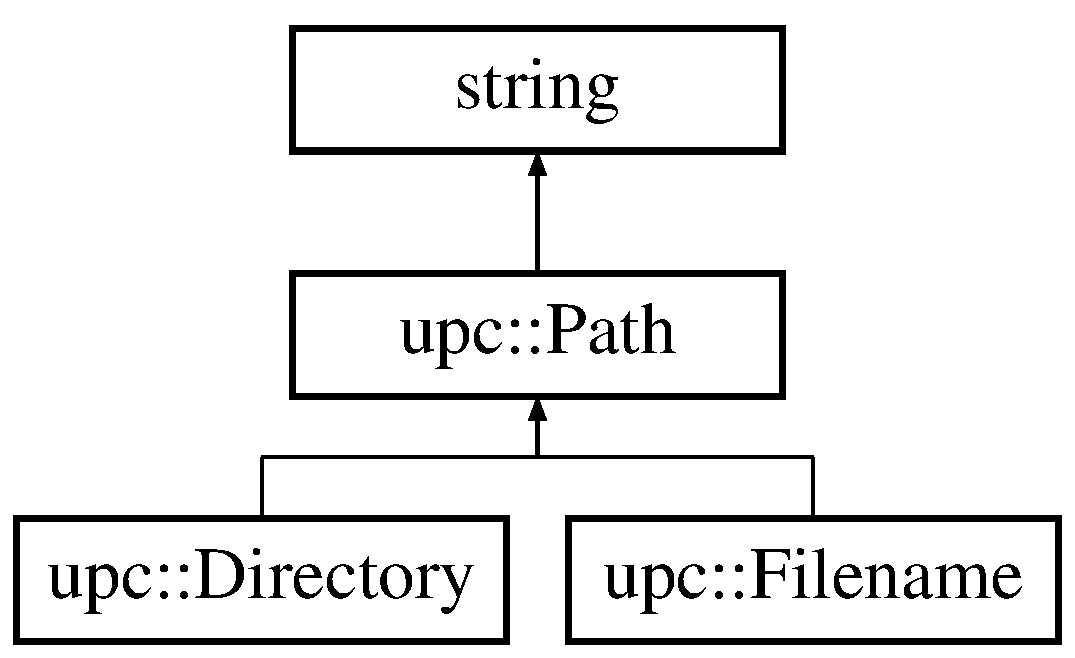
\includegraphics[height=3.000000cm]{classupc_1_1Path}
\end{center}
\end{figure}
\subsection*{Public Member Functions}
\begin{DoxyCompactItemize}
\item 
\hyperlink{classupc_1_1Path_a0bf9cbf155aa8e6b39a49acedbd4bb9a}{Path} ()
\item 
\hyperlink{classupc_1_1Path_a364200f9a453fedd5ba68f79f8b93154}{Path} (const string \&str)
\item 
\hyperlink{classupc_1_1Path_a082270e960275af46d65c3ce252ef581}{Path} (const char $\ast$str)
\item 
virtual \hyperlink{classupc_1_1Path_a96f9ce2d43d4544b663316abb32281a1}{$\sim$\+Path} ()
\end{DoxyCompactItemize}


\subsection{Constructor \& Destructor Documentation}
\index{upc\+::\+Path@{upc\+::\+Path}!Path@{Path}}
\index{Path@{Path}!upc\+::\+Path@{upc\+::\+Path}}
\subsubsection[{\texorpdfstring{Path()}{Path()}}]{\setlength{\rightskip}{0pt plus 5cm}upc\+::\+Path\+::\+Path (
\begin{DoxyParamCaption}
{}
\end{DoxyParamCaption}
)\hspace{0.3cm}{\ttfamily [inline]}}\hypertarget{classupc_1_1Path_a0bf9cbf155aa8e6b39a49acedbd4bb9a}{}\label{classupc_1_1Path_a0bf9cbf155aa8e6b39a49acedbd4bb9a}
\index{upc\+::\+Path@{upc\+::\+Path}!Path@{Path}}
\index{Path@{Path}!upc\+::\+Path@{upc\+::\+Path}}
\subsubsection[{\texorpdfstring{Path(const string \&str)}{Path(const string &str)}}]{\setlength{\rightskip}{0pt plus 5cm}upc\+::\+Path\+::\+Path (
\begin{DoxyParamCaption}
\item[{const string \&}]{str}
\end{DoxyParamCaption}
)\hspace{0.3cm}{\ttfamily [inline]}}\hypertarget{classupc_1_1Path_a364200f9a453fedd5ba68f79f8b93154}{}\label{classupc_1_1Path_a364200f9a453fedd5ba68f79f8b93154}
\index{upc\+::\+Path@{upc\+::\+Path}!Path@{Path}}
\index{Path@{Path}!upc\+::\+Path@{upc\+::\+Path}}
\subsubsection[{\texorpdfstring{Path(const char $\ast$str)}{Path(const char *str)}}]{\setlength{\rightskip}{0pt plus 5cm}upc\+::\+Path\+::\+Path (
\begin{DoxyParamCaption}
\item[{const char $\ast$}]{str}
\end{DoxyParamCaption}
)\hspace{0.3cm}{\ttfamily [inline]}}\hypertarget{classupc_1_1Path_a082270e960275af46d65c3ce252ef581}{}\label{classupc_1_1Path_a082270e960275af46d65c3ce252ef581}
\index{upc\+::\+Path@{upc\+::\+Path}!````~Path@{$\sim$\+Path}}
\index{````~Path@{$\sim$\+Path}!upc\+::\+Path@{upc\+::\+Path}}
\subsubsection[{\texorpdfstring{$\sim$\+Path()}{~Path()}}]{\setlength{\rightskip}{0pt plus 5cm}virtual upc\+::\+Path\+::$\sim$\+Path (
\begin{DoxyParamCaption}
{}
\end{DoxyParamCaption}
)\hspace{0.3cm}{\ttfamily [inline]}, {\ttfamily [virtual]}}\hypertarget{classupc_1_1Path_a96f9ce2d43d4544b663316abb32281a1}{}\label{classupc_1_1Path_a96f9ce2d43d4544b663316abb32281a1}


The documentation for this class was generated from the following file\+:\begin{DoxyCompactItemize}
\item 
include/\hyperlink{filename_8h}{filename.\+h}\end{DoxyCompactItemize}

\hypertarget{classupc_1_1PitchAnalyzer}{}\section{upc\+:\+:Pitch\+Analyzer Class Reference}
\label{classupc_1_1PitchAnalyzer}\index{upc\+::\+Pitch\+Analyzer@{upc\+::\+Pitch\+Analyzer}}


{\ttfamily \#include $<$pitch\+\_\+analyzer.\+h$>$}

\subsection*{Public Types}
\begin{DoxyCompactItemize}
\item 
enum \hyperlink{classupc_1_1PitchAnalyzer_ab82b7694d6bc72839e5be6e526be81b6}{Window} \{ \hyperlink{classupc_1_1PitchAnalyzer_ab82b7694d6bc72839e5be6e526be81b6ae89513dddf240af8bbef3358597f244c}{R\+E\+CT}, 
\hyperlink{classupc_1_1PitchAnalyzer_ab82b7694d6bc72839e5be6e526be81b6a20e793e736a503aacbed0294970a9b33}{H\+A\+M\+M\+I\+NG}
 \}
\end{DoxyCompactItemize}
\subsection*{Public Member Functions}
\begin{DoxyCompactItemize}
\item 
void \hyperlink{classupc_1_1PitchAnalyzer_a96cc042a650825b25ca39c41beebd0db}{set\+\_\+window} (\hyperlink{classupc_1_1PitchAnalyzer_ab82b7694d6bc72839e5be6e526be81b6}{Window} type)
\begin{DoxyCompactList}\small\item\em Window type. \end{DoxyCompactList}\item 
\hyperlink{classupc_1_1PitchAnalyzer_ae7cfb918feadd7d56f5736e4ef600c06}{Pitch\+Analyzer} (unsigned int f\+Len, unsigned int s\+Freq, \hyperlink{classupc_1_1PitchAnalyzer_ab82b7694d6bc72839e5be6e526be81b6}{Window} w=\hyperlink{classupc_1_1PitchAnalyzer_ab82b7694d6bc72839e5be6e526be81b6a20e793e736a503aacbed0294970a9b33}{Pitch\+Analyzer\+::\+H\+A\+M\+M\+I\+NG}, \hyperlink{FFTReal__readme_8txt_a0ea2fae2a8106200bf378b90eae003cf}{float} min\+\_\+\+F0=\hyperlink{namespaceupc_ae8ed4ce6dc2c05dfc1aa6432db41e1ae}{M\+I\+N\+\_\+\+F0}, \hyperlink{FFTReal__readme_8txt_a0ea2fae2a8106200bf378b90eae003cf}{float} max\+\_\+\+F0=\hyperlink{namespaceupc_ab69be42753266b6e1a0deaa8eba56a19}{M\+A\+X\+\_\+\+F0})
\begin{DoxyCompactList}\small\item\em true if the frame is unvoiced \end{DoxyCompactList}\item 
\hyperlink{FFTReal__readme_8txt_a0ea2fae2a8106200bf378b90eae003cf}{float} \hyperlink{classupc_1_1PitchAnalyzer_a2cd33d0cbfc699c43f570442190ca9e6}{operator()} (const std\+::vector$<$ \hyperlink{FFTReal__readme_8txt_a0ea2fae2a8106200bf378b90eae003cf}{float} $>$ \&\+\_\+x) const 
\item 
\hyperlink{FFTReal__readme_8txt_a0ea2fae2a8106200bf378b90eae003cf}{float} \hyperlink{classupc_1_1PitchAnalyzer_a00aef276755224ed20668f3b1b3f16d1}{operator()} (const \hyperlink{FFTReal__readme_8txt_a0ea2fae2a8106200bf378b90eae003cf}{float} $\ast$pt, unsigned int \hyperlink{FFTReal__readme_8txt_a049dd452c22185832440207517cffdaa}{N}) const 
\item 
\hyperlink{FFTReal__readme_8txt_a0ea2fae2a8106200bf378b90eae003cf}{float} \hyperlink{classupc_1_1PitchAnalyzer_a2f924f9f45df090463be1498518934ab}{operator()} (std\+::vector$<$ \hyperlink{FFTReal__readme_8txt_a0ea2fae2a8106200bf378b90eae003cf}{float} $>$\+::const\+\_\+iterator begin, std\+::vector$<$ \hyperlink{FFTReal__readme_8txt_a0ea2fae2a8106200bf378b90eae003cf}{float} $>$\+::const\+\_\+iterator end) const 
\item 
void \hyperlink{classupc_1_1PitchAnalyzer_ac33887654b62b3f90c3de231ec187d94}{set\+\_\+f0\+\_\+range} (\hyperlink{FFTReal__readme_8txt_a0ea2fae2a8106200bf378b90eae003cf}{float} min\+\_\+\+F0, \hyperlink{FFTReal__readme_8txt_a0ea2fae2a8106200bf378b90eae003cf}{float} max\+\_\+\+F0)
\end{DoxyCompactItemize}
\subsection*{Private Member Functions}
\begin{DoxyCompactItemize}
\item 
void \hyperlink{classupc_1_1PitchAnalyzer_a45da4fa8b3d7bd67d87468a3153a839e}{autocorrelation} (const std\+::vector$<$ \hyperlink{FFTReal__readme_8txt_a0ea2fae2a8106200bf378b90eae003cf}{float} $>$ \&\hyperlink{FFTReal__readme_8txt_a9c92ac89d1560f812393ca39a19e581e}{x}, std\+::vector$<$ \hyperlink{FFTReal__readme_8txt_a0ea2fae2a8106200bf378b90eae003cf}{float} $>$ \&r) const 
\begin{DoxyCompactList}\small\item\em max. value of pitch period, in samples \end{DoxyCompactList}\item 
\hyperlink{FFTReal__readme_8txt_a0ea2fae2a8106200bf378b90eae003cf}{float} \hyperlink{classupc_1_1PitchAnalyzer_abb8bc34c74953c8d43127fe4acb6b4eb}{compute\+\_\+pitch} (std\+::vector$<$ \hyperlink{FFTReal__readme_8txt_a0ea2fae2a8106200bf378b90eae003cf}{float} $>$ \&\hyperlink{FFTReal__readme_8txt_a9c92ac89d1560f812393ca39a19e581e}{x}) const 
\begin{DoxyCompactList}\small\item\em compute correlation from lag=0 to r.\+size() \end{DoxyCompactList}\item 
bool \hyperlink{classupc_1_1PitchAnalyzer_a0b32960107336078d87118cb10d6c83f}{unvoiced} (\hyperlink{FFTReal__readme_8txt_a0ea2fae2a8106200bf378b90eae003cf}{float} pot, \hyperlink{FFTReal__readme_8txt_a0ea2fae2a8106200bf378b90eae003cf}{float} r1norm, \hyperlink{FFTReal__readme_8txt_a0ea2fae2a8106200bf378b90eae003cf}{float} rmaxnorm) const 
\begin{DoxyCompactList}\small\item\em Returns the pitch (in Hz) of input frame x. \end{DoxyCompactList}\end{DoxyCompactItemize}
\subsection*{Private Attributes}
\begin{DoxyCompactItemize}
\item 
std\+::vector$<$ \hyperlink{FFTReal__readme_8txt_a0ea2fae2a8106200bf378b90eae003cf}{float} $>$ \hyperlink{classupc_1_1PitchAnalyzer_aa9531a6af11904dca47a18cc22c4bcdd}{window}
\begin{DoxyCompactList}\small\item\em pre-\/compute window \end{DoxyCompactList}\item 
unsigned int \hyperlink{classupc_1_1PitchAnalyzer_a6ef737140140ec94f7be345804f28c73}{frame\+Len}
\begin{DoxyCompactList}\small\item\em precomputed window \end{DoxyCompactList}\item 
unsigned int \hyperlink{classupc_1_1PitchAnalyzer_a92578165c78c763749ef5c8aa23b1ca2}{sampling\+Freq}
\begin{DoxyCompactList}\small\item\em length of frame (ins samples). Has to be set in the constructor call \end{DoxyCompactList}\item 
unsigned int \hyperlink{classupc_1_1PitchAnalyzer_a3bb67370dbd69fade6be12fdae510eed}{npitch\+\_\+min}
\begin{DoxyCompactList}\small\item\em sampling rate (ins samples). Has to be set in the constructor call \end{DoxyCompactList}\item 
unsigned int \hyperlink{classupc_1_1PitchAnalyzer_a63d4cf285fa5f7a4e579ac2e02d36dd2}{npitch\+\_\+max}
\begin{DoxyCompactList}\small\item\em min. value of pitch period, in samples \end{DoxyCompactList}\end{DoxyCompactItemize}


\subsection{Detailed Description}
\hyperlink{classupc_1_1PitchAnalyzer}{Pitch\+Analyzer}\+: class that computes the pitch (in Hz) from a signal frame. No pre-\/processing or post-\/processing has been included 

\subsection{Member Enumeration Documentation}
\index{upc\+::\+Pitch\+Analyzer@{upc\+::\+Pitch\+Analyzer}!Window@{Window}}
\index{Window@{Window}!upc\+::\+Pitch\+Analyzer@{upc\+::\+Pitch\+Analyzer}}
\subsubsection[{\texorpdfstring{Window}{Window}}]{\setlength{\rightskip}{0pt plus 5cm}enum {\bf upc\+::\+Pitch\+Analyzer\+::\+Window}}\hypertarget{classupc_1_1PitchAnalyzer_ab82b7694d6bc72839e5be6e526be81b6}{}\label{classupc_1_1PitchAnalyzer_ab82b7694d6bc72839e5be6e526be81b6}
\begin{Desc}
\item[Enumerator]\par
\begin{description}
\index{R\+E\+CT@{R\+E\+CT}!upc\+::\+Pitch\+Analyzer@{upc\+::\+Pitch\+Analyzer}}\index{upc\+::\+Pitch\+Analyzer@{upc\+::\+Pitch\+Analyzer}!R\+E\+CT@{R\+E\+CT}}\item[{\em 
R\+E\+CT\hypertarget{classupc_1_1PitchAnalyzer_ab82b7694d6bc72839e5be6e526be81b6ae89513dddf240af8bbef3358597f244c}{}\label{classupc_1_1PitchAnalyzer_ab82b7694d6bc72839e5be6e526be81b6ae89513dddf240af8bbef3358597f244c}
}]\index{H\+A\+M\+M\+I\+NG@{H\+A\+M\+M\+I\+NG}!upc\+::\+Pitch\+Analyzer@{upc\+::\+Pitch\+Analyzer}}\index{upc\+::\+Pitch\+Analyzer@{upc\+::\+Pitch\+Analyzer}!H\+A\+M\+M\+I\+NG@{H\+A\+M\+M\+I\+NG}}\item[{\em 
H\+A\+M\+M\+I\+NG\hypertarget{classupc_1_1PitchAnalyzer_ab82b7694d6bc72839e5be6e526be81b6a20e793e736a503aacbed0294970a9b33}{}\label{classupc_1_1PitchAnalyzer_ab82b7694d6bc72839e5be6e526be81b6a20e793e736a503aacbed0294970a9b33}
}]\end{description}
\end{Desc}


\subsection{Constructor \& Destructor Documentation}
\index{upc\+::\+Pitch\+Analyzer@{upc\+::\+Pitch\+Analyzer}!Pitch\+Analyzer@{Pitch\+Analyzer}}
\index{Pitch\+Analyzer@{Pitch\+Analyzer}!upc\+::\+Pitch\+Analyzer@{upc\+::\+Pitch\+Analyzer}}
\subsubsection[{\texorpdfstring{Pitch\+Analyzer(unsigned int f\+Len, unsigned int s\+Freq, Window w=\+Pitch\+Analyzer\+::\+H\+A\+M\+M\+I\+N\+G, float min\+\_\+\+F0=\+M\+I\+N\+\_\+\+F0, float max\+\_\+\+F0=\+M\+A\+X\+\_\+\+F0)}{PitchAnalyzer(unsigned int fLen, unsigned int sFreq, Window w=PitchAnalyzer::HAMMING, float min_F0=MIN_F0, float max_F0=MAX_F0)}}]{\setlength{\rightskip}{0pt plus 5cm}upc\+::\+Pitch\+Analyzer\+::\+Pitch\+Analyzer (
\begin{DoxyParamCaption}
\item[{unsigned int}]{f\+Len, }
\item[{unsigned int}]{s\+Freq, }
\item[{{\bf Window}}]{w = {\ttfamily {\bf Pitch\+Analyzer\+::\+H\+A\+M\+M\+I\+NG}}, }
\item[{{\bf float}}]{min\+\_\+\+F0 = {\ttfamily {\bf M\+I\+N\+\_\+\+F0}}, }
\item[{{\bf float}}]{max\+\_\+\+F0 = {\ttfamily {\bf M\+A\+X\+\_\+\+F0}}}
\end{DoxyParamCaption}
)\hspace{0.3cm}{\ttfamily [inline]}}\hypertarget{classupc_1_1PitchAnalyzer_ae7cfb918feadd7d56f5736e4ef600c06}{}\label{classupc_1_1PitchAnalyzer_ae7cfb918feadd7d56f5736e4ef600c06}


true if the frame is unvoiced 

Declaration of the \hyperlink{classupc_1_1PitchAnalyzer}{Pitch\+Analyzer}\+: f\+Len\+: frame length, in samples s\+Freq\+: sampling rate (samples/second) w\+: window type min\+\_\+\+F0, max\+\_\+\+F0\+: the pitch range can be restricted to this range 

\subsection{Member Function Documentation}
\index{upc\+::\+Pitch\+Analyzer@{upc\+::\+Pitch\+Analyzer}!autocorrelation@{autocorrelation}}
\index{autocorrelation@{autocorrelation}!upc\+::\+Pitch\+Analyzer@{upc\+::\+Pitch\+Analyzer}}
\subsubsection[{\texorpdfstring{autocorrelation(const std\+::vector$<$ float $>$ \&x, std\+::vector$<$ float $>$ \&r) const }{autocorrelation(const std::vector< float > &x, std::vector< float > &r) const }}]{\setlength{\rightskip}{0pt plus 5cm}void upc\+::\+Pitch\+Analyzer\+::autocorrelation (
\begin{DoxyParamCaption}
\item[{const std\+::vector$<$ {\bf float} $>$ \&}]{x, }
\item[{std\+::vector$<$ {\bf float} $>$ \&}]{r}
\end{DoxyParamCaption}
) const\hspace{0.3cm}{\ttfamily [private]}}\hypertarget{classupc_1_1PitchAnalyzer_a45da4fa8b3d7bd67d87468a3153a839e}{}\label{classupc_1_1PitchAnalyzer_a45da4fa8b3d7bd67d87468a3153a839e}


max. value of pitch period, in samples 

\index{upc\+::\+Pitch\+Analyzer@{upc\+::\+Pitch\+Analyzer}!compute\+\_\+pitch@{compute\+\_\+pitch}}
\index{compute\+\_\+pitch@{compute\+\_\+pitch}!upc\+::\+Pitch\+Analyzer@{upc\+::\+Pitch\+Analyzer}}
\subsubsection[{\texorpdfstring{compute\+\_\+pitch(std\+::vector$<$ float $>$ \&x) const }{compute_pitch(std::vector< float > &x) const }}]{\setlength{\rightskip}{0pt plus 5cm}{\bf float} upc\+::\+Pitch\+Analyzer\+::compute\+\_\+pitch (
\begin{DoxyParamCaption}
\item[{std\+::vector$<$ {\bf float} $>$ \&}]{x}
\end{DoxyParamCaption}
) const\hspace{0.3cm}{\ttfamily [private]}}\hypertarget{classupc_1_1PitchAnalyzer_abb8bc34c74953c8d43127fe4acb6b4eb}{}\label{classupc_1_1PitchAnalyzer_abb8bc34c74953c8d43127fe4acb6b4eb}


compute correlation from lag=0 to r.\+size() 

\index{upc\+::\+Pitch\+Analyzer@{upc\+::\+Pitch\+Analyzer}!operator()@{operator()}}
\index{operator()@{operator()}!upc\+::\+Pitch\+Analyzer@{upc\+::\+Pitch\+Analyzer}}
\subsubsection[{\texorpdfstring{operator()(const std\+::vector$<$ float $>$ \&\+\_\+x) const }{operator()(const std::vector< float > &_x) const }}]{\setlength{\rightskip}{0pt plus 5cm}{\bf float} upc\+::\+Pitch\+Analyzer\+::operator() (
\begin{DoxyParamCaption}
\item[{const std\+::vector$<$ {\bf float} $>$ \&}]{\+\_\+x}
\end{DoxyParamCaption}
) const\hspace{0.3cm}{\ttfamily [inline]}}\hypertarget{classupc_1_1PitchAnalyzer_a2cd33d0cbfc699c43f570442190ca9e6}{}\label{classupc_1_1PitchAnalyzer_a2cd33d0cbfc699c43f570442190ca9e6}
Operator () \+: compute the pitch for the given vector x \index{upc\+::\+Pitch\+Analyzer@{upc\+::\+Pitch\+Analyzer}!operator()@{operator()}}
\index{operator()@{operator()}!upc\+::\+Pitch\+Analyzer@{upc\+::\+Pitch\+Analyzer}}
\subsubsection[{\texorpdfstring{operator()(const float $\ast$pt, unsigned int N) const }{operator()(const float *pt, unsigned int N) const }}]{\setlength{\rightskip}{0pt plus 5cm}{\bf float} upc\+::\+Pitch\+Analyzer\+::operator() (
\begin{DoxyParamCaption}
\item[{const {\bf float} $\ast$}]{pt, }
\item[{unsigned int}]{N}
\end{DoxyParamCaption}
) const\hspace{0.3cm}{\ttfamily [inline]}}\hypertarget{classupc_1_1PitchAnalyzer_a00aef276755224ed20668f3b1b3f16d1}{}\label{classupc_1_1PitchAnalyzer_a00aef276755224ed20668f3b1b3f16d1}
Operator () \+: compute the pitch for the given \char`\"{}\+C\char`\"{} vector (float $\ast$). N is the size of the vector pointer by pt. copy input values into local vector x \index{upc\+::\+Pitch\+Analyzer@{upc\+::\+Pitch\+Analyzer}!operator()@{operator()}}
\index{operator()@{operator()}!upc\+::\+Pitch\+Analyzer@{upc\+::\+Pitch\+Analyzer}}
\subsubsection[{\texorpdfstring{operator()(std\+::vector$<$ float $>$\+::const\+\_\+iterator begin, std\+::vector$<$ float $>$\+::const\+\_\+iterator end) const }{operator()(std::vector< float >::const_iterator begin, std::vector< float >::const_iterator end) const }}]{\setlength{\rightskip}{0pt plus 5cm}{\bf float} upc\+::\+Pitch\+Analyzer\+::operator() (
\begin{DoxyParamCaption}
\item[{std\+::vector$<$ {\bf float} $>$\+::const\+\_\+iterator}]{begin, }
\item[{std\+::vector$<$ {\bf float} $>$\+::const\+\_\+iterator}]{end}
\end{DoxyParamCaption}
) const\hspace{0.3cm}{\ttfamily [inline]}}\hypertarget{classupc_1_1PitchAnalyzer_a2f924f9f45df090463be1498518934ab}{}\label{classupc_1_1PitchAnalyzer_a2f924f9f45df090463be1498518934ab}
Operator () \+: compute the pitch for the given vector, expressed by the begin and end iterators copy input values into local vector x \index{upc\+::\+Pitch\+Analyzer@{upc\+::\+Pitch\+Analyzer}!set\+\_\+f0\+\_\+range@{set\+\_\+f0\+\_\+range}}
\index{set\+\_\+f0\+\_\+range@{set\+\_\+f0\+\_\+range}!upc\+::\+Pitch\+Analyzer@{upc\+::\+Pitch\+Analyzer}}
\subsubsection[{\texorpdfstring{set\+\_\+f0\+\_\+range(float min\+\_\+\+F0, float max\+\_\+\+F0)}{set_f0_range(float min_F0, float max_F0)}}]{\setlength{\rightskip}{0pt plus 5cm}void upc\+::\+Pitch\+Analyzer\+::set\+\_\+f0\+\_\+range (
\begin{DoxyParamCaption}
\item[{{\bf float}}]{min\+\_\+\+F0, }
\item[{{\bf float}}]{max\+\_\+\+F0}
\end{DoxyParamCaption}
)}\hypertarget{classupc_1_1PitchAnalyzer_ac33887654b62b3f90c3de231ec187d94}{}\label{classupc_1_1PitchAnalyzer_ac33887654b62b3f90c3de231ec187d94}
Set pitch range; (input in Hz, npitch\+\_\+min and npitch\+\_\+max, in samples \index{upc\+::\+Pitch\+Analyzer@{upc\+::\+Pitch\+Analyzer}!set\+\_\+window@{set\+\_\+window}}
\index{set\+\_\+window@{set\+\_\+window}!upc\+::\+Pitch\+Analyzer@{upc\+::\+Pitch\+Analyzer}}
\subsubsection[{\texorpdfstring{set\+\_\+window(\+Window type)}{set_window(Window type)}}]{\setlength{\rightskip}{0pt plus 5cm}void upc\+::\+Pitch\+Analyzer\+::set\+\_\+window (
\begin{DoxyParamCaption}
\item[{{\bf Window}}]{type}
\end{DoxyParamCaption}
)}\hypertarget{classupc_1_1PitchAnalyzer_a96cc042a650825b25ca39c41beebd0db}{}\label{classupc_1_1PitchAnalyzer_a96cc042a650825b25ca39c41beebd0db}


Window type. 

\index{upc\+::\+Pitch\+Analyzer@{upc\+::\+Pitch\+Analyzer}!unvoiced@{unvoiced}}
\index{unvoiced@{unvoiced}!upc\+::\+Pitch\+Analyzer@{upc\+::\+Pitch\+Analyzer}}
\subsubsection[{\texorpdfstring{unvoiced(float pot, float r1norm, float rmaxnorm) const }{unvoiced(float pot, float r1norm, float rmaxnorm) const }}]{\setlength{\rightskip}{0pt plus 5cm}bool upc\+::\+Pitch\+Analyzer\+::unvoiced (
\begin{DoxyParamCaption}
\item[{{\bf float}}]{pot, }
\item[{{\bf float}}]{r1norm, }
\item[{{\bf float}}]{rmaxnorm}
\end{DoxyParamCaption}
) const\hspace{0.3cm}{\ttfamily [private]}}\hypertarget{classupc_1_1PitchAnalyzer_a0b32960107336078d87118cb10d6c83f}{}\label{classupc_1_1PitchAnalyzer_a0b32960107336078d87118cb10d6c83f}


Returns the pitch (in Hz) of input frame x. 



\subsection{Member Data Documentation}
\index{upc\+::\+Pitch\+Analyzer@{upc\+::\+Pitch\+Analyzer}!frame\+Len@{frame\+Len}}
\index{frame\+Len@{frame\+Len}!upc\+::\+Pitch\+Analyzer@{upc\+::\+Pitch\+Analyzer}}
\subsubsection[{\texorpdfstring{frame\+Len}{frameLen}}]{\setlength{\rightskip}{0pt plus 5cm}unsigned int upc\+::\+Pitch\+Analyzer\+::frame\+Len\hspace{0.3cm}{\ttfamily [private]}}\hypertarget{classupc_1_1PitchAnalyzer_a6ef737140140ec94f7be345804f28c73}{}\label{classupc_1_1PitchAnalyzer_a6ef737140140ec94f7be345804f28c73}


precomputed window 

\index{upc\+::\+Pitch\+Analyzer@{upc\+::\+Pitch\+Analyzer}!npitch\+\_\+max@{npitch\+\_\+max}}
\index{npitch\+\_\+max@{npitch\+\_\+max}!upc\+::\+Pitch\+Analyzer@{upc\+::\+Pitch\+Analyzer}}
\subsubsection[{\texorpdfstring{npitch\+\_\+max}{npitch_max}}]{\setlength{\rightskip}{0pt plus 5cm}unsigned int upc\+::\+Pitch\+Analyzer\+::npitch\+\_\+max\hspace{0.3cm}{\ttfamily [private]}}\hypertarget{classupc_1_1PitchAnalyzer_a63d4cf285fa5f7a4e579ac2e02d36dd2}{}\label{classupc_1_1PitchAnalyzer_a63d4cf285fa5f7a4e579ac2e02d36dd2}


min. value of pitch period, in samples 

\index{upc\+::\+Pitch\+Analyzer@{upc\+::\+Pitch\+Analyzer}!npitch\+\_\+min@{npitch\+\_\+min}}
\index{npitch\+\_\+min@{npitch\+\_\+min}!upc\+::\+Pitch\+Analyzer@{upc\+::\+Pitch\+Analyzer}}
\subsubsection[{\texorpdfstring{npitch\+\_\+min}{npitch_min}}]{\setlength{\rightskip}{0pt plus 5cm}unsigned int upc\+::\+Pitch\+Analyzer\+::npitch\+\_\+min\hspace{0.3cm}{\ttfamily [private]}}\hypertarget{classupc_1_1PitchAnalyzer_a3bb67370dbd69fade6be12fdae510eed}{}\label{classupc_1_1PitchAnalyzer_a3bb67370dbd69fade6be12fdae510eed}


sampling rate (ins samples). Has to be set in the constructor call 

\index{upc\+::\+Pitch\+Analyzer@{upc\+::\+Pitch\+Analyzer}!sampling\+Freq@{sampling\+Freq}}
\index{sampling\+Freq@{sampling\+Freq}!upc\+::\+Pitch\+Analyzer@{upc\+::\+Pitch\+Analyzer}}
\subsubsection[{\texorpdfstring{sampling\+Freq}{samplingFreq}}]{\setlength{\rightskip}{0pt plus 5cm}unsigned int upc\+::\+Pitch\+Analyzer\+::sampling\+Freq\hspace{0.3cm}{\ttfamily [private]}}\hypertarget{classupc_1_1PitchAnalyzer_a92578165c78c763749ef5c8aa23b1ca2}{}\label{classupc_1_1PitchAnalyzer_a92578165c78c763749ef5c8aa23b1ca2}


length of frame (ins samples). Has to be set in the constructor call 

\index{upc\+::\+Pitch\+Analyzer@{upc\+::\+Pitch\+Analyzer}!window@{window}}
\index{window@{window}!upc\+::\+Pitch\+Analyzer@{upc\+::\+Pitch\+Analyzer}}
\subsubsection[{\texorpdfstring{window}{window}}]{\setlength{\rightskip}{0pt plus 5cm}std\+::vector$<${\bf float}$>$ upc\+::\+Pitch\+Analyzer\+::window\hspace{0.3cm}{\ttfamily [private]}}\hypertarget{classupc_1_1PitchAnalyzer_aa9531a6af11904dca47a18cc22c4bcdd}{}\label{classupc_1_1PitchAnalyzer_aa9531a6af11904dca47a18cc22c4bcdd}


pre-\/compute window 



The documentation for this class was generated from the following files\+:\begin{DoxyCompactItemize}
\item 
get\+\_\+pitch/\hyperlink{pitch__analyzer_8h}{pitch\+\_\+analyzer.\+h}\item 
get\+\_\+pitch/\hyperlink{pitch__analyzer_8cpp}{pitch\+\_\+analyzer.\+cpp}\end{DoxyCompactItemize}

\hypertarget{structVAD__DATA}{}\section{V\+A\+D\+\_\+\+D\+A\+TA Struct Reference}
\label{structVAD__DATA}\index{V\+A\+D\+\_\+\+D\+A\+TA@{V\+A\+D\+\_\+\+D\+A\+TA}}


{\ttfamily \#include $<$vad.\+h$>$}

\subsection*{Public Attributes}
\begin{DoxyCompactItemize}
\item 
\hyperlink{vad_8h_a655a5d992101d81e27b861d90c712d65}{V\+A\+D\+\_\+\+S\+T\+A\+TE} \hyperlink{structVAD__DATA_a02d71db9de6c2438820ea1cfab9187bf}{state}
\item 
\hyperlink{FFTReal__readme_8txt_a0ea2fae2a8106200bf378b90eae003cf}{float} \hyperlink{structVAD__DATA_ad2b4da91b7353a41a0fe64e65093e056}{sampling\+\_\+rate}
\item 
unsigned int \hyperlink{structVAD__DATA_a24ae8d2d4e2c13f0c930cb281ddf5ae5}{frame\+\_\+length}
\item 
\hyperlink{FFTReal__readme_8txt_a0ea2fae2a8106200bf378b90eae003cf}{float} \hyperlink{structVAD__DATA_a73be3c4f2bddba51db3f74d1df7b9286}{last\+\_\+feature}
\end{DoxyCompactItemize}


\subsection{Member Data Documentation}
\index{V\+A\+D\+\_\+\+D\+A\+TA@{V\+A\+D\+\_\+\+D\+A\+TA}!frame\+\_\+length@{frame\+\_\+length}}
\index{frame\+\_\+length@{frame\+\_\+length}!V\+A\+D\+\_\+\+D\+A\+TA@{V\+A\+D\+\_\+\+D\+A\+TA}}
\subsubsection[{\texorpdfstring{frame\+\_\+length}{frame_length}}]{\setlength{\rightskip}{0pt plus 5cm}unsigned int V\+A\+D\+\_\+\+D\+A\+T\+A\+::frame\+\_\+length}\hypertarget{structVAD__DATA_a24ae8d2d4e2c13f0c930cb281ddf5ae5}{}\label{structVAD__DATA_a24ae8d2d4e2c13f0c930cb281ddf5ae5}
\index{V\+A\+D\+\_\+\+D\+A\+TA@{V\+A\+D\+\_\+\+D\+A\+TA}!last\+\_\+feature@{last\+\_\+feature}}
\index{last\+\_\+feature@{last\+\_\+feature}!V\+A\+D\+\_\+\+D\+A\+TA@{V\+A\+D\+\_\+\+D\+A\+TA}}
\subsubsection[{\texorpdfstring{last\+\_\+feature}{last_feature}}]{\setlength{\rightskip}{0pt plus 5cm}{\bf float} V\+A\+D\+\_\+\+D\+A\+T\+A\+::last\+\_\+feature}\hypertarget{structVAD__DATA_a73be3c4f2bddba51db3f74d1df7b9286}{}\label{structVAD__DATA_a73be3c4f2bddba51db3f74d1df7b9286}
\index{V\+A\+D\+\_\+\+D\+A\+TA@{V\+A\+D\+\_\+\+D\+A\+TA}!sampling\+\_\+rate@{sampling\+\_\+rate}}
\index{sampling\+\_\+rate@{sampling\+\_\+rate}!V\+A\+D\+\_\+\+D\+A\+TA@{V\+A\+D\+\_\+\+D\+A\+TA}}
\subsubsection[{\texorpdfstring{sampling\+\_\+rate}{sampling_rate}}]{\setlength{\rightskip}{0pt plus 5cm}{\bf float} V\+A\+D\+\_\+\+D\+A\+T\+A\+::sampling\+\_\+rate}\hypertarget{structVAD__DATA_ad2b4da91b7353a41a0fe64e65093e056}{}\label{structVAD__DATA_ad2b4da91b7353a41a0fe64e65093e056}
\index{V\+A\+D\+\_\+\+D\+A\+TA@{V\+A\+D\+\_\+\+D\+A\+TA}!state@{state}}
\index{state@{state}!V\+A\+D\+\_\+\+D\+A\+TA@{V\+A\+D\+\_\+\+D\+A\+TA}}
\subsubsection[{\texorpdfstring{state}{state}}]{\setlength{\rightskip}{0pt plus 5cm}{\bf V\+A\+D\+\_\+\+S\+T\+A\+TE} V\+A\+D\+\_\+\+D\+A\+T\+A\+::state}\hypertarget{structVAD__DATA_a02d71db9de6c2438820ea1cfab9187bf}{}\label{structVAD__DATA_a02d71db9de6c2438820ea1cfab9187bf}


The documentation for this struct was generated from the following file\+:\begin{DoxyCompactItemize}
\item 
include/\hyperlink{vad_8h}{vad.\+h}\end{DoxyCompactItemize}

\chapter{File Documentation}
\hypertarget{get__pitch_8cpp}{}\section{get\+\_\+pitch/get\+\_\+pitch.cpp File Reference}
\label{get__pitch_8cpp}\index{get\+\_\+pitch/get\+\_\+pitch.\+cpp@{get\+\_\+pitch/get\+\_\+pitch.\+cpp}}
{\ttfamily \#include $<$iostream$>$}\\*
{\ttfamily \#include $<$fstream$>$}\\*
{\ttfamily \#include \char`\"{}wavfile\+\_\+mono.\+h\char`\"{}}\\*
{\ttfamily \#include \char`\"{}pitch\+\_\+analyzer.\+h\char`\"{}}\\*
\subsection*{Macros}
\begin{DoxyCompactItemize}
\item 
\#define \hyperlink{get__pitch_8cpp_a7d356b7d5a77c1e2fb7e8154f65ebfcf}{F\+R\+A\+M\+E\+\_\+\+L\+EN}~0.\+030 /$\ast$ 30 ms. $\ast$/
\item 
\#define \hyperlink{get__pitch_8cpp_a69ba23fac7d991d8e893ea34ef05ba00}{F\+R\+A\+M\+E\+\_\+\+S\+H\+I\+FT}~0.\+015 /$\ast$ 15 ms. $\ast$/
\end{DoxyCompactItemize}
\subsection*{Functions}
\begin{DoxyCompactItemize}
\item 
int \hyperlink{get__pitch_8cpp_ac0f2228420376f4db7e1274f2b41667c}{main} (int argc, const char $\ast$argv\mbox{[}$\,$\mbox{]})
\end{DoxyCompactItemize}


\subsection{Macro Definition Documentation}
\index{get\+\_\+pitch.\+cpp@{get\+\_\+pitch.\+cpp}!F\+R\+A\+M\+E\+\_\+\+L\+EN@{F\+R\+A\+M\+E\+\_\+\+L\+EN}}
\index{F\+R\+A\+M\+E\+\_\+\+L\+EN@{F\+R\+A\+M\+E\+\_\+\+L\+EN}!get\+\_\+pitch.\+cpp@{get\+\_\+pitch.\+cpp}}
\subsubsection[{\texorpdfstring{F\+R\+A\+M\+E\+\_\+\+L\+EN}{FRAME_LEN}}]{\setlength{\rightskip}{0pt plus 5cm}\#define F\+R\+A\+M\+E\+\_\+\+L\+EN~0.\+030 /$\ast$ 30 ms. $\ast$/}\hypertarget{get__pitch_8cpp_a7d356b7d5a77c1e2fb7e8154f65ebfcf}{}\label{get__pitch_8cpp_a7d356b7d5a77c1e2fb7e8154f65ebfcf}
\index{get\+\_\+pitch.\+cpp@{get\+\_\+pitch.\+cpp}!F\+R\+A\+M\+E\+\_\+\+S\+H\+I\+FT@{F\+R\+A\+M\+E\+\_\+\+S\+H\+I\+FT}}
\index{F\+R\+A\+M\+E\+\_\+\+S\+H\+I\+FT@{F\+R\+A\+M\+E\+\_\+\+S\+H\+I\+FT}!get\+\_\+pitch.\+cpp@{get\+\_\+pitch.\+cpp}}
\subsubsection[{\texorpdfstring{F\+R\+A\+M\+E\+\_\+\+S\+H\+I\+FT}{FRAME_SHIFT}}]{\setlength{\rightskip}{0pt plus 5cm}\#define F\+R\+A\+M\+E\+\_\+\+S\+H\+I\+FT~0.\+015 /$\ast$ 15 ms. $\ast$/}\hypertarget{get__pitch_8cpp_a69ba23fac7d991d8e893ea34ef05ba00}{}\label{get__pitch_8cpp_a69ba23fac7d991d8e893ea34ef05ba00}


\subsection{Function Documentation}
\index{get\+\_\+pitch.\+cpp@{get\+\_\+pitch.\+cpp}!main@{main}}
\index{main@{main}!get\+\_\+pitch.\+cpp@{get\+\_\+pitch.\+cpp}}
\subsubsection[{\texorpdfstring{main(int argc, const char $\ast$argv[])}{main(int argc, const char *argv[])}}]{\setlength{\rightskip}{0pt plus 5cm}int main (
\begin{DoxyParamCaption}
\item[{int}]{argc, }
\item[{const char $\ast$}]{argv\mbox{[}$\,$\mbox{]}}
\end{DoxyParamCaption}
)}\hypertarget{get__pitch_8cpp_ac0f2228420376f4db7e1274f2b41667c}{}\label{get__pitch_8cpp_ac0f2228420376f4db7e1274f2b41667c}
Main program\+: Arguments\+:
\begin{DoxyItemize}
\item input (wav) file
\item output (txt) file with f0 one value per line with the f0 for each frame (or 0 for unvoiced frames) 
\end{DoxyItemize}Read input sound file

Define analyzer

You can preprocess the input data x ....

Iterate for each frame and save values in f0 vector

Write f0 contour into the output file 
\hypertarget{pitch__analyzer_8cpp}{}\section{get\+\_\+pitch/pitch\+\_\+analyzer.cpp File Reference}
\label{pitch__analyzer_8cpp}\index{get\+\_\+pitch/pitch\+\_\+analyzer.\+cpp@{get\+\_\+pitch/pitch\+\_\+analyzer.\+cpp}}
{\ttfamily \#include $<$iostream$>$}\\*
{\ttfamily \#include $<$math.\+h$>$}\\*
{\ttfamily \#include \char`\"{}pitch\+\_\+analyzer.\+h\char`\"{}}\\*
\subsection*{Namespaces}
\begin{DoxyCompactItemize}
\item 
 \hyperlink{namespaceupc}{upc}
\end{DoxyCompactItemize}

\hypertarget{pitch__analyzer_8h}{}\section{get\+\_\+pitch/pitch\+\_\+analyzer.h File Reference}
\label{pitch__analyzer_8h}\index{get\+\_\+pitch/pitch\+\_\+analyzer.\+h@{get\+\_\+pitch/pitch\+\_\+analyzer.\+h}}
{\ttfamily \#include $<$vector$>$}\\*
{\ttfamily \#include $<$algorithm$>$}\\*
\subsection*{Classes}
\begin{DoxyCompactItemize}
\item 
class \hyperlink{classupc_1_1PitchAnalyzer}{upc\+::\+Pitch\+Analyzer}
\end{DoxyCompactItemize}
\subsection*{Namespaces}
\begin{DoxyCompactItemize}
\item 
 \hyperlink{namespaceupc}{upc}
\end{DoxyCompactItemize}
\subsection*{Variables}
\begin{DoxyCompactItemize}
\item 
const \hyperlink{FFTReal__readme_8txt_a0ea2fae2a8106200bf378b90eae003cf}{float} \hyperlink{namespaceupc_ae8ed4ce6dc2c05dfc1aa6432db41e1ae}{upc\+::\+M\+I\+N\+\_\+\+F0} =20.\+0F
\item 
const \hyperlink{FFTReal__readme_8txt_a0ea2fae2a8106200bf378b90eae003cf}{float} \hyperlink{namespaceupc_ab69be42753266b6e1a0deaa8eba56a19}{upc\+::\+M\+A\+X\+\_\+\+F0} =10000.\+0F
\end{DoxyCompactItemize}

\hypertarget{pitch__evaluate_8cpp}{}\section{get\+\_\+pitch/pitch\+\_\+evaluate.cpp File Reference}
\label{pitch__evaluate_8cpp}\index{get\+\_\+pitch/pitch\+\_\+evaluate.\+cpp@{get\+\_\+pitch/pitch\+\_\+evaluate.\+cpp}}
{\ttfamily \#include $<$iostream$>$}\\*
{\ttfamily \#include $<$fstream$>$}\\*
{\ttfamily \#include $<$iomanip$>$}\\*
{\ttfamily \#include $<$vector$>$}\\*
{\ttfamily \#include $<$math.\+h$>$}\\*
{\ttfamily \#include $<$stdlib.\+h$>$}\\*
\subsection*{Functions}
\begin{DoxyCompactItemize}
\item 
int \hyperlink{pitch__evaluate_8cpp_acc47b8492bcbc1ad3fab7d6ac74d2d8d}{read\+\_\+vector} (const string \&filename, vector$<$ \hyperlink{FFTReal__readme_8txt_a0ea2fae2a8106200bf378b90eae003cf}{float} $>$ \&\hyperlink{FFTReal__readme_8txt_a9c92ac89d1560f812393ca39a19e581e}{x})
\item 
void \hyperlink{pitch__evaluate_8cpp_a77944b5af41e256ec0ba1f00442cf9ba}{compare} (const vector$<$ \hyperlink{FFTReal__readme_8txt_a0ea2fae2a8106200bf378b90eae003cf}{float} $>$ \&vref, const vector$<$ \hyperlink{FFTReal__readme_8txt_a0ea2fae2a8106200bf378b90eae003cf}{float} $>$ \&vtest, int \&num\+\_\+voiced, int \&num\+\_\+unvoiced, int \&num\+\_\+voiced\+\_\+unvoiced, int \&num\+\_\+unvoiced\+\_\+voiced, int \&num\+\_\+voiced\+\_\+voiced, int \&num\+\_\+gross\+\_\+errors, \hyperlink{FFTReal__readme_8txt_a0ea2fae2a8106200bf378b90eae003cf}{float} \&fine\+\_\+error)
\item 
void \hyperlink{pitch__evaluate_8cpp_a87c47e482c3ef68d841885d5f81166a6}{print\+\_\+results} (int nframes, int num\+\_\+voiced, int num\+\_\+unvoiced, int num\+\_\+voiced\+\_\+unvoiced, int num\+\_\+unvoiced\+\_\+voiced, int num\+\_\+voiced\+\_\+voiced, int num\+\_\+gross\+\_\+errors, \hyperlink{FFTReal__readme_8txt_a0ea2fae2a8106200bf378b90eae003cf}{float} fine\+\_\+error)
\item 
int \hyperlink{pitch__evaluate_8cpp_ac0f2228420376f4db7e1274f2b41667c}{main} (int argc, const char $\ast$argv\mbox{[}$\,$\mbox{]})
\end{DoxyCompactItemize}
\subsection*{Variables}
\begin{DoxyCompactItemize}
\item 
const \hyperlink{FFTReal__readme_8txt_a0ea2fae2a8106200bf378b90eae003cf}{float} \hyperlink{pitch__evaluate_8cpp_ac3e1e3eb989b9766a74a68f946c1b20d}{gross\+\_\+threshold} = 0.\+2F
\end{DoxyCompactItemize}


\subsection{Function Documentation}
\index{pitch\+\_\+evaluate.\+cpp@{pitch\+\_\+evaluate.\+cpp}!compare@{compare}}
\index{compare@{compare}!pitch\+\_\+evaluate.\+cpp@{pitch\+\_\+evaluate.\+cpp}}
\subsubsection[{\texorpdfstring{compare(const vector$<$ float $>$ \&vref, const vector$<$ float $>$ \&vtest, int \&num\+\_\+voiced, int \&num\+\_\+unvoiced, int \&num\+\_\+voiced\+\_\+unvoiced, int \&num\+\_\+unvoiced\+\_\+voiced, int \&num\+\_\+voiced\+\_\+voiced, int \&num\+\_\+gross\+\_\+errors, float \&fine\+\_\+error)}{compare(const vector< float > &vref, const vector< float > &vtest, int &num_voiced, int &num_unvoiced, int &num_voiced_unvoiced, int &num_unvoiced_voiced, int &num_voiced_voiced, int &num_gross_errors, float &fine_error)}}]{\setlength{\rightskip}{0pt plus 5cm}void compare (
\begin{DoxyParamCaption}
\item[{const vector$<$ {\bf float} $>$ \&}]{vref, }
\item[{const vector$<$ {\bf float} $>$ \&}]{vtest, }
\item[{int \&}]{num\+\_\+voiced, }
\item[{int \&}]{num\+\_\+unvoiced, }
\item[{int \&}]{num\+\_\+voiced\+\_\+unvoiced, }
\item[{int \&}]{num\+\_\+unvoiced\+\_\+voiced, }
\item[{int \&}]{num\+\_\+voiced\+\_\+voiced, }
\item[{int \&}]{num\+\_\+gross\+\_\+errors, }
\item[{{\bf float} \&}]{fine\+\_\+error}
\end{DoxyParamCaption}
)}\hypertarget{pitch__evaluate_8cpp_a77944b5af41e256ec0ba1f00442cf9ba}{}\label{pitch__evaluate_8cpp_a77944b5af41e256ec0ba1f00442cf9ba}
\index{pitch\+\_\+evaluate.\+cpp@{pitch\+\_\+evaluate.\+cpp}!main@{main}}
\index{main@{main}!pitch\+\_\+evaluate.\+cpp@{pitch\+\_\+evaluate.\+cpp}}
\subsubsection[{\texorpdfstring{main(int argc, const char $\ast$argv[])}{main(int argc, const char *argv[])}}]{\setlength{\rightskip}{0pt plus 5cm}int main (
\begin{DoxyParamCaption}
\item[{int}]{argc, }
\item[{const char $\ast$}]{argv\mbox{[}$\,$\mbox{]}}
\end{DoxyParamCaption}
)}\hypertarget{pitch__evaluate_8cpp_ac0f2228420376f4db7e1274f2b41667c}{}\label{pitch__evaluate_8cpp_ac0f2228420376f4db7e1274f2b41667c}
\index{pitch\+\_\+evaluate.\+cpp@{pitch\+\_\+evaluate.\+cpp}!print\+\_\+results@{print\+\_\+results}}
\index{print\+\_\+results@{print\+\_\+results}!pitch\+\_\+evaluate.\+cpp@{pitch\+\_\+evaluate.\+cpp}}
\subsubsection[{\texorpdfstring{print\+\_\+results(int nframes, int num\+\_\+voiced, int num\+\_\+unvoiced, int num\+\_\+voiced\+\_\+unvoiced, int num\+\_\+unvoiced\+\_\+voiced, int num\+\_\+voiced\+\_\+voiced, int num\+\_\+gross\+\_\+errors, float fine\+\_\+error)}{print_results(int nframes, int num_voiced, int num_unvoiced, int num_voiced_unvoiced, int num_unvoiced_voiced, int num_voiced_voiced, int num_gross_errors, float fine_error)}}]{\setlength{\rightskip}{0pt plus 5cm}void print\+\_\+results (
\begin{DoxyParamCaption}
\item[{int}]{nframes, }
\item[{int}]{num\+\_\+voiced, }
\item[{int}]{num\+\_\+unvoiced, }
\item[{int}]{num\+\_\+voiced\+\_\+unvoiced, }
\item[{int}]{num\+\_\+unvoiced\+\_\+voiced, }
\item[{int}]{num\+\_\+voiced\+\_\+voiced, }
\item[{int}]{num\+\_\+gross\+\_\+errors, }
\item[{{\bf float}}]{fine\+\_\+error}
\end{DoxyParamCaption}
)}\hypertarget{pitch__evaluate_8cpp_a87c47e482c3ef68d841885d5f81166a6}{}\label{pitch__evaluate_8cpp_a87c47e482c3ef68d841885d5f81166a6}
\index{pitch\+\_\+evaluate.\+cpp@{pitch\+\_\+evaluate.\+cpp}!read\+\_\+vector@{read\+\_\+vector}}
\index{read\+\_\+vector@{read\+\_\+vector}!pitch\+\_\+evaluate.\+cpp@{pitch\+\_\+evaluate.\+cpp}}
\subsubsection[{\texorpdfstring{read\+\_\+vector(const string \&filename, vector$<$ float $>$ \&x)}{read_vector(const string &filename, vector< float > &x)}}]{\setlength{\rightskip}{0pt plus 5cm}int read\+\_\+vector (
\begin{DoxyParamCaption}
\item[{const string \&}]{filename, }
\item[{vector$<$ {\bf float} $>$ \&}]{x}
\end{DoxyParamCaption}
)}\hypertarget{pitch__evaluate_8cpp_acc47b8492bcbc1ad3fab7d6ac74d2d8d}{}\label{pitch__evaluate_8cpp_acc47b8492bcbc1ad3fab7d6ac74d2d8d}


\subsection{Variable Documentation}
\index{pitch\+\_\+evaluate.\+cpp@{pitch\+\_\+evaluate.\+cpp}!gross\+\_\+threshold@{gross\+\_\+threshold}}
\index{gross\+\_\+threshold@{gross\+\_\+threshold}!pitch\+\_\+evaluate.\+cpp@{pitch\+\_\+evaluate.\+cpp}}
\subsubsection[{\texorpdfstring{gross\+\_\+threshold}{gross_threshold}}]{\setlength{\rightskip}{0pt plus 5cm}const {\bf float} gross\+\_\+threshold = 0.\+2F}\hypertarget{pitch__evaluate_8cpp_ac3e1e3eb989b9766a74a68f946c1b20d}{}\label{pitch__evaluate_8cpp_ac3e1e3eb989b9766a74a68f946c1b20d}

\hypertarget{digital__filter_8h}{}\section{include/digital\+\_\+filter.h File Reference}
\label{digital__filter_8h}\index{include/digital\+\_\+filter.\+h@{include/digital\+\_\+filter.\+h}}
{\ttfamily \#include $<$vector$>$}\\*
\subsection*{Classes}
\begin{DoxyCompactItemize}
\item 
class \hyperlink{classupc_1_1CircularIndex}{upc\+::\+Circular\+Index}
\begin{DoxyCompactList}\small\item\em Circular Index used to go through state circular buffer (u) \end{DoxyCompactList}\item 
class \hyperlink{classupc_1_1DigitalFilter}{upc\+::\+Digital\+Filter}
\begin{DoxyCompactList}\small\item\em Digital filter implemented using direct form. \end{DoxyCompactList}\end{DoxyCompactItemize}
\subsection*{Namespaces}
\begin{DoxyCompactItemize}
\item 
 \hyperlink{namespaceupc}{upc}
\end{DoxyCompactItemize}

\hypertarget{def_8h}{}\section{include/ffft/def.h File Reference}
\label{def_8h}\index{include/ffft/def.\+h@{include/ffft/def.\+h}}
\subsection*{Namespaces}
\begin{DoxyCompactItemize}
\item 
 \hyperlink{namespaceffft}{ffft}
\end{DoxyCompactItemize}
\subsection*{Macros}
\begin{DoxyCompactItemize}
\item 
\#define \hyperlink{def_8h_a31b2ada863c9efa7455efae4e13661f3}{ffft\+\_\+\+F\+O\+R\+C\+E\+I\+N\+L\+I\+NE}~inline
\end{DoxyCompactItemize}
\subsection*{Variables}
\begin{DoxyCompactItemize}
\item 
const double \hyperlink{namespaceffft_a74ffcd4c90202b5240bbca7374dfd6fa}{ffft\+::\+PI} = 3.\+1415926535897932384626433832795
\item 
const double \hyperlink{namespaceffft_a489004390ad7d791bf53a724c0f07abb}{ffft\+::\+S\+Q\+R\+T2} = 1.\+41421356237309514547462185873883
\end{DoxyCompactItemize}


\subsection{Macro Definition Documentation}
\index{def.\+h@{def.\+h}!ffft\+\_\+\+F\+O\+R\+C\+E\+I\+N\+L\+I\+NE@{ffft\+\_\+\+F\+O\+R\+C\+E\+I\+N\+L\+I\+NE}}
\index{ffft\+\_\+\+F\+O\+R\+C\+E\+I\+N\+L\+I\+NE@{ffft\+\_\+\+F\+O\+R\+C\+E\+I\+N\+L\+I\+NE}!def.\+h@{def.\+h}}
\subsubsection[{\texorpdfstring{ffft\+\_\+\+F\+O\+R\+C\+E\+I\+N\+L\+I\+NE}{ffft_FORCEINLINE}}]{\setlength{\rightskip}{0pt plus 5cm}\#define ffft\+\_\+\+F\+O\+R\+C\+E\+I\+N\+L\+I\+NE~inline}\hypertarget{def_8h_a31b2ada863c9efa7455efae4e13661f3}{}\label{def_8h_a31b2ada863c9efa7455efae4e13661f3}

\hypertarget{DynArray_8h}{}\section{include/ffft/\+Dyn\+Array.h File Reference}
\label{DynArray_8h}\index{include/ffft/\+Dyn\+Array.\+h@{include/ffft/\+Dyn\+Array.\+h}}
{\ttfamily \#include \char`\"{}ffft/\+Dyn\+Array.\+hpp\char`\"{}}\\*
\subsection*{Classes}
\begin{DoxyCompactItemize}
\item 
class \hyperlink{classffft_1_1DynArray}{ffft\+::\+Dyn\+Array$<$ T $>$}
\end{DoxyCompactItemize}
\subsection*{Namespaces}
\begin{DoxyCompactItemize}
\item 
 \hyperlink{namespaceffft}{ffft}
\end{DoxyCompactItemize}

\hypertarget{DynArray_8hpp}{}\section{include/ffft/\+Dyn\+Array.hpp File Reference}
\label{DynArray_8hpp}\index{include/ffft/\+Dyn\+Array.\+hpp@{include/ffft/\+Dyn\+Array.\+hpp}}
{\ttfamily \#include $<$cassert$>$}\\*
\subsection*{Namespaces}
\begin{DoxyCompactItemize}
\item 
 \hyperlink{namespaceffft}{ffft}
\end{DoxyCompactItemize}
\subsection*{Macros}
\begin{DoxyCompactItemize}
\item 
\#define \hyperlink{DynArray_8hpp_ad74efcb6a9d581885aa6775982c07997}{ffft\+\_\+\+Dyn\+Array\+\_\+\+C\+U\+R\+R\+E\+N\+T\+\_\+\+C\+O\+D\+E\+H\+E\+A\+D\+ER}
\item 
\#define \hyperlink{DynArray_8hpp_a86200f79a6a46453b3f096c370e0ae16}{ffft\+\_\+\+Dyn\+Array\+\_\+\+C\+O\+D\+E\+H\+E\+A\+D\+E\+R\+\_\+\+I\+N\+C\+L\+U\+D\+ED}
\end{DoxyCompactItemize}


\subsection{Macro Definition Documentation}
\index{Dyn\+Array.\+hpp@{Dyn\+Array.\+hpp}!ffft\+\_\+\+Dyn\+Array\+\_\+\+C\+O\+D\+E\+H\+E\+A\+D\+E\+R\+\_\+\+I\+N\+C\+L\+U\+D\+ED@{ffft\+\_\+\+Dyn\+Array\+\_\+\+C\+O\+D\+E\+H\+E\+A\+D\+E\+R\+\_\+\+I\+N\+C\+L\+U\+D\+ED}}
\index{ffft\+\_\+\+Dyn\+Array\+\_\+\+C\+O\+D\+E\+H\+E\+A\+D\+E\+R\+\_\+\+I\+N\+C\+L\+U\+D\+ED@{ffft\+\_\+\+Dyn\+Array\+\_\+\+C\+O\+D\+E\+H\+E\+A\+D\+E\+R\+\_\+\+I\+N\+C\+L\+U\+D\+ED}!Dyn\+Array.\+hpp@{Dyn\+Array.\+hpp}}
\subsubsection[{\texorpdfstring{ffft\+\_\+\+Dyn\+Array\+\_\+\+C\+O\+D\+E\+H\+E\+A\+D\+E\+R\+\_\+\+I\+N\+C\+L\+U\+D\+ED}{ffft_DynArray_CODEHEADER_INCLUDED}}]{\setlength{\rightskip}{0pt plus 5cm}\#define ffft\+\_\+\+Dyn\+Array\+\_\+\+C\+O\+D\+E\+H\+E\+A\+D\+E\+R\+\_\+\+I\+N\+C\+L\+U\+D\+ED}\hypertarget{DynArray_8hpp_a86200f79a6a46453b3f096c370e0ae16}{}\label{DynArray_8hpp_a86200f79a6a46453b3f096c370e0ae16}
\index{Dyn\+Array.\+hpp@{Dyn\+Array.\+hpp}!ffft\+\_\+\+Dyn\+Array\+\_\+\+C\+U\+R\+R\+E\+N\+T\+\_\+\+C\+O\+D\+E\+H\+E\+A\+D\+ER@{ffft\+\_\+\+Dyn\+Array\+\_\+\+C\+U\+R\+R\+E\+N\+T\+\_\+\+C\+O\+D\+E\+H\+E\+A\+D\+ER}}
\index{ffft\+\_\+\+Dyn\+Array\+\_\+\+C\+U\+R\+R\+E\+N\+T\+\_\+\+C\+O\+D\+E\+H\+E\+A\+D\+ER@{ffft\+\_\+\+Dyn\+Array\+\_\+\+C\+U\+R\+R\+E\+N\+T\+\_\+\+C\+O\+D\+E\+H\+E\+A\+D\+ER}!Dyn\+Array.\+hpp@{Dyn\+Array.\+hpp}}
\subsubsection[{\texorpdfstring{ffft\+\_\+\+Dyn\+Array\+\_\+\+C\+U\+R\+R\+E\+N\+T\+\_\+\+C\+O\+D\+E\+H\+E\+A\+D\+ER}{ffft_DynArray_CURRENT_CODEHEADER}}]{\setlength{\rightskip}{0pt plus 5cm}\#define ffft\+\_\+\+Dyn\+Array\+\_\+\+C\+U\+R\+R\+E\+N\+T\+\_\+\+C\+O\+D\+E\+H\+E\+A\+D\+ER}\hypertarget{DynArray_8hpp_ad74efcb6a9d581885aa6775982c07997}{}\label{DynArray_8hpp_ad74efcb6a9d581885aa6775982c07997}

\hypertarget{FFTReal_8h}{}\section{include/ffft/\+F\+F\+T\+Real.h File Reference}
\label{FFTReal_8h}\index{include/ffft/\+F\+F\+T\+Real.\+h@{include/ffft/\+F\+F\+T\+Real.\+h}}
{\ttfamily \#include \char`\"{}ffft/def.\+h\char`\"{}}\\*
{\ttfamily \#include \char`\"{}ffft/\+Dyn\+Array.\+h\char`\"{}}\\*
{\ttfamily \#include \char`\"{}ffft/\+Osc\+Sin\+Cos.\+h\char`\"{}}\\*
{\ttfamily \#include \char`\"{}ffft/\+F\+F\+T\+Real.\+hpp\char`\"{}}\\*
\subsection*{Classes}
\begin{DoxyCompactItemize}
\item 
class \hyperlink{classffft_1_1FFTReal}{ffft\+::\+F\+F\+T\+Real$<$ D\+T $>$}
\end{DoxyCompactItemize}
\subsection*{Namespaces}
\begin{DoxyCompactItemize}
\item 
 \hyperlink{namespaceffft}{ffft}
\end{DoxyCompactItemize}

\hypertarget{FFTReal_8hpp}{}\section{include/ffft/\+F\+F\+T\+Real.hpp File Reference}
\label{FFTReal_8hpp}\index{include/ffft/\+F\+F\+T\+Real.\+hpp@{include/ffft/\+F\+F\+T\+Real.\+hpp}}
{\ttfamily \#include $<$cassert$>$}\\*
{\ttfamily \#include $<$cmath$>$}\\*
\subsection*{Namespaces}
\begin{DoxyCompactItemize}
\item 
 \hyperlink{namespaceffft}{ffft}
\end{DoxyCompactItemize}
\subsection*{Macros}
\begin{DoxyCompactItemize}
\item 
\#define \hyperlink{FFTReal_8hpp_a7e1c53e720f689723accc78c4835f91c}{ffft\+\_\+\+F\+F\+T\+Real\+\_\+\+C\+U\+R\+R\+E\+N\+T\+\_\+\+C\+O\+D\+E\+H\+E\+A\+D\+ER}
\item 
\#define \hyperlink{FFTReal_8hpp_adf3b5663ee12a1d9e612686163e7ad52}{ffft\+\_\+\+F\+F\+T\+Real\+\_\+\+C\+O\+D\+E\+H\+E\+A\+D\+E\+R\+\_\+\+I\+N\+C\+L\+U\+D\+ED}
\end{DoxyCompactItemize}


\subsection{Macro Definition Documentation}
\index{F\+F\+T\+Real.\+hpp@{F\+F\+T\+Real.\+hpp}!ffft\+\_\+\+F\+F\+T\+Real\+\_\+\+C\+O\+D\+E\+H\+E\+A\+D\+E\+R\+\_\+\+I\+N\+C\+L\+U\+D\+ED@{ffft\+\_\+\+F\+F\+T\+Real\+\_\+\+C\+O\+D\+E\+H\+E\+A\+D\+E\+R\+\_\+\+I\+N\+C\+L\+U\+D\+ED}}
\index{ffft\+\_\+\+F\+F\+T\+Real\+\_\+\+C\+O\+D\+E\+H\+E\+A\+D\+E\+R\+\_\+\+I\+N\+C\+L\+U\+D\+ED@{ffft\+\_\+\+F\+F\+T\+Real\+\_\+\+C\+O\+D\+E\+H\+E\+A\+D\+E\+R\+\_\+\+I\+N\+C\+L\+U\+D\+ED}!F\+F\+T\+Real.\+hpp@{F\+F\+T\+Real.\+hpp}}
\subsubsection[{\texorpdfstring{ffft\+\_\+\+F\+F\+T\+Real\+\_\+\+C\+O\+D\+E\+H\+E\+A\+D\+E\+R\+\_\+\+I\+N\+C\+L\+U\+D\+ED}{ffft_FFTReal_CODEHEADER_INCLUDED}}]{\setlength{\rightskip}{0pt plus 5cm}\#define ffft\+\_\+\+F\+F\+T\+Real\+\_\+\+C\+O\+D\+E\+H\+E\+A\+D\+E\+R\+\_\+\+I\+N\+C\+L\+U\+D\+ED}\hypertarget{FFTReal_8hpp_adf3b5663ee12a1d9e612686163e7ad52}{}\label{FFTReal_8hpp_adf3b5663ee12a1d9e612686163e7ad52}
\index{F\+F\+T\+Real.\+hpp@{F\+F\+T\+Real.\+hpp}!ffft\+\_\+\+F\+F\+T\+Real\+\_\+\+C\+U\+R\+R\+E\+N\+T\+\_\+\+C\+O\+D\+E\+H\+E\+A\+D\+ER@{ffft\+\_\+\+F\+F\+T\+Real\+\_\+\+C\+U\+R\+R\+E\+N\+T\+\_\+\+C\+O\+D\+E\+H\+E\+A\+D\+ER}}
\index{ffft\+\_\+\+F\+F\+T\+Real\+\_\+\+C\+U\+R\+R\+E\+N\+T\+\_\+\+C\+O\+D\+E\+H\+E\+A\+D\+ER@{ffft\+\_\+\+F\+F\+T\+Real\+\_\+\+C\+U\+R\+R\+E\+N\+T\+\_\+\+C\+O\+D\+E\+H\+E\+A\+D\+ER}!F\+F\+T\+Real.\+hpp@{F\+F\+T\+Real.\+hpp}}
\subsubsection[{\texorpdfstring{ffft\+\_\+\+F\+F\+T\+Real\+\_\+\+C\+U\+R\+R\+E\+N\+T\+\_\+\+C\+O\+D\+E\+H\+E\+A\+D\+ER}{ffft_FFTReal_CURRENT_CODEHEADER}}]{\setlength{\rightskip}{0pt plus 5cm}\#define ffft\+\_\+\+F\+F\+T\+Real\+\_\+\+C\+U\+R\+R\+E\+N\+T\+\_\+\+C\+O\+D\+E\+H\+E\+A\+D\+ER}\hypertarget{FFTReal_8hpp_a7e1c53e720f689723accc78c4835f91c}{}\label{FFTReal_8hpp_a7e1c53e720f689723accc78c4835f91c}

\hypertarget{FFTReal__readme_8txt}{}\section{include/ffft/\+F\+F\+T\+Real\+\_\+readme.txt File Reference}
\label{FFTReal__readme_8txt}\index{include/ffft/\+F\+F\+T\+Real\+\_\+readme.\+txt@{include/ffft/\+F\+F\+T\+Real\+\_\+readme.\+txt}}
{\ttfamily \#include \char`\"{}ffft/\+F\+F\+T\+Real.\+h\char`\"{}}\\*
{\ttfamily \#include \char`\"{}ffft/\+F\+F\+T\+Real\+Fix\+Len.\+h\char`\"{}}\\*
\subsection*{Typedefs}
\begin{DoxyCompactItemize}
\item 
using \hyperlink{FFTReal__readme_8txt_a555609f588a3dd8483e643133ba24b82}{len} = 1024
\end{DoxyCompactItemize}
\subsection*{Functions}
\begin{DoxyCompactItemize}
\item 
\hyperlink{classffft_1_1FFTReal}{ffft\+::\+F\+F\+T\+Real}$<$ \hyperlink{FFTReal__readme_8txt_a0ea2fae2a8106200bf378b90eae003cf}{float} $>$ \hyperlink{FFTReal__readme_8txt_a38b2d99092edb3ec444550a95aa1951f}{fft\+\_\+object} (\hyperlink{FFTReal__readme_8txt_a555609f588a3dd8483e643133ba24b82}{len})
\item 
\hyperlink{FFTReal__readme_8txt_a38b2d99092edb3ec444550a95aa1951f}{fft\+\_\+object} \hyperlink{FFTReal__readme_8txt_a601296d1e380b29c96683b649d7d1518}{do\+\_\+fft} (\hyperlink{FFTReal__readme_8txt_abbf3cc73d1e3e4714ab1639819396eca}{f}, \hyperlink{FFTReal__readme_8txt_a9c92ac89d1560f812393ca39a19e581e}{x})
\item 
\hyperlink{FFTReal__readme_8txt_a38b2d99092edb3ec444550a95aa1951f}{fft\+\_\+object} \hyperlink{FFTReal__readme_8txt_a1a33a3b7245f269d5150c436da7d5ed6}{do\+\_\+ifft} (\hyperlink{FFTReal__readme_8txt_abbf3cc73d1e3e4714ab1639819396eca}{f}, \hyperlink{FFTReal__readme_8txt_a9c92ac89d1560f812393ca39a19e581e}{x})
\item 
\hyperlink{FFTReal__readme_8txt_a38b2d99092edb3ec444550a95aa1951f}{fft\+\_\+object} \hyperlink{FFTReal__readme_8txt_ab87096300f2c26c87aa35b0623fdfd1e}{rescale} (\hyperlink{FFTReal__readme_8txt_a9c92ac89d1560f812393ca39a19e581e}{x})
\item 
Warning depending on the compiler and its optimisation options If compilation time is too encapsulate the F\+FT \hyperlink{FFTReal__readme_8txt_a5057f8d0a8b36ba2bdea206a5592c87a}{object} in a seprate \hyperlink{FFTReal__readme_8txt_ad229ab5c8241df85a2096743cc8c4e9f}{class} whose header doesn t need to include F\+F\+T\+Real\+Fix\+Len \hyperlink{FFTReal__readme_8txt_a5a475fe9e77e2d776b063abc32a10e20}{h} so you just have to compile the wrapper once and only link it the other times For \hyperlink{FFTReal__readme_8txt_a22165307fc7fb8edc069828217b871ec}{example} (quick, dirty and incomplete)
\end{DoxyCompactItemize}
\subsection*{Variables}
\begin{DoxyCompactItemize}
\item 
it can be changed by modifying the Data\+Type typedef in F\+F\+T\+Real\+Fix\+Len\+Param \hyperlink{FFTReal__readme_8txt_a5a475fe9e77e2d776b063abc32a10e20}{h} As \hyperlink{FFTReal__readme_8txt_afc545541c7ab0be25cf239418fc47b65}{F\+F\+T\+Real} \hyperlink{FFTReal__readme_8txt_ad229ab5c8241df85a2096743cc8c4e9f}{class}
\item 
it can be changed by modifying the Data\+Type typedef in F\+F\+T\+Real\+Fix\+Len\+Param \hyperlink{FFTReal__readme_8txt_a5a475fe9e77e2d776b063abc32a10e20}{h} As \hyperlink{FFTReal__readme_8txt_afc545541c7ab0be25cf239418fc47b65}{F\+F\+T\+Real} it supports only floating point types or equivalent Use is similar as the one of \hyperlink{FFTReal__readme_8txt_afc545541c7ab0be25cf239418fc47b65}{F\+F\+T\+Real} To instanciate the \hyperlink{FFTReal__readme_8txt_a5057f8d0a8b36ba2bdea206a5592c87a}{object}
\item 
it can be changed by modifying the Data\+Type typedef in F\+F\+T\+Real\+Fix\+Len\+Param \hyperlink{FFTReal__readme_8txt_a5a475fe9e77e2d776b063abc32a10e20}{h} As \hyperlink{FFTReal__readme_8txt_afc545541c7ab0be25cf239418fc47b65}{F\+F\+T\+Real} it supports only floating point types or equivalent Use is similar as the one of \hyperlink{FFTReal__readme_8txt_afc545541c7ab0be25cf239418fc47b65}{F\+F\+T\+Real} To instanciate the just proceed as indicated \hyperlink{FFTReal__readme_8txt_aadd6d22385a49baac7311a220729ab52}{below}
\item 
some of them are of particular \hyperlink{FFTReal__readme_8txt_a8dd124b3ee508be769f386edc2b8ccc7}{interest}
\item 
some of them are of particular length fixed at run time ffft F\+F\+T\+Real\+Fix\+Len \hyperlink{FFTReal__readme_8txt_a5a475fe9e77e2d776b063abc32a10e20}{h}
\item 
some of them are of particular length fixed at run time ffft F\+F\+T\+Real\+Fix\+Len length fixed at compile time delphi \hyperlink{FFTReal__readme_8txt_afc545541c7ab0be25cf239418fc47b65}{F\+F\+T\+Real} \hyperlink{FFTReal__readme_8txt_a6cf8b214cfb6bfb689594a776ceb1ea0}{pas}
\item 
Then you can use this \hyperlink{FFTReal__readme_8txt_a5057f8d0a8b36ba2bdea206a5592c87a}{object} to compute as many F\+F\+Ts and I\+F\+F\+Ts as you want They will be computed very quickly because a lot of work has been done in the \hyperlink{FFTReal__readme_8txt_a5057f8d0a8b36ba2bdea206a5592c87a}{object} construction \hyperlink{FFTReal__readme_8txt_a0ea2fae2a8106200bf378b90eae003cf}{float} \hyperlink{FFTReal__readme_8txt_a9c92ac89d1560f812393ca39a19e581e}{x} \mbox{[}1024\mbox{]}
\item 
\hyperlink{FFTReal__readme_8txt_a0ea2fae2a8106200bf378b90eae003cf}{float} \hyperlink{FFTReal__readme_8txt_abbf3cc73d1e3e4714ab1639819396eca}{f} \mbox{[}1024\mbox{]}
\item 
\hyperlink{FFTReal__readme_8txt_a9c92ac89d1560f812393ca39a19e581e}{x}\mbox{[}$\,$\mbox{]} and \hyperlink{FFTReal__readme_8txt_abbf3cc73d1e3e4714ab1639819396eca}{f}\mbox{[}$\,$\mbox{]} are floating point number arrays \hyperlink{FFTReal__readme_8txt_a9c92ac89d1560f812393ca39a19e581e}{x}\mbox{[}$\,$\mbox{]} is the real number sequence which we want to compute the F\+FT \hyperlink{FFTReal__readme_8txt_abbf3cc73d1e3e4714ab1639819396eca}{f}\mbox{[}$\,$\mbox{]} is the \hyperlink{FFTReal__readme_8txt_af64dcf51fedf6a89308c7e46c0868511}{result}
\item 
\hyperlink{FFTReal__readme_8txt_a9c92ac89d1560f812393ca39a19e581e}{x}\mbox{[}$\,$\mbox{]} and \hyperlink{FFTReal__readme_8txt_abbf3cc73d1e3e4714ab1639819396eca}{f}\mbox{[}$\,$\mbox{]} are floating point number arrays \hyperlink{FFTReal__readme_8txt_a9c92ac89d1560f812393ca39a19e581e}{x}\mbox{[}$\,$\mbox{]} is the real number sequence which we want to compute the F\+FT \hyperlink{FFTReal__readme_8txt_abbf3cc73d1e3e4714ab1639819396eca}{f}\mbox{[}$\,$\mbox{]} is the in the frequency domain \hyperlink{FFTReal__readme_8txt_abbf3cc73d1e3e4714ab1639819396eca}{f} has the same number of elements as but \hyperlink{FFTReal__readme_8txt_abbf3cc73d1e3e4714ab1639819396eca}{f}\mbox{[}$\,$\mbox{]} elements are complex numbers The routine uses some F\+FT properties to optimize memory and to reduce \hyperlink{FFTReal__readme_8txt_a65cbf8e61482778d7aa2ebe890cc7d7c}{calculations}
\item 
\hyperlink{FFTReal__readme_8txt_a9c92ac89d1560f812393ca39a19e581e}{x}\mbox{[}$\,$\mbox{]} and \hyperlink{FFTReal__readme_8txt_abbf3cc73d1e3e4714ab1639819396eca}{f}\mbox{[}$\,$\mbox{]} are floating point number arrays \hyperlink{FFTReal__readme_8txt_a9c92ac89d1560f812393ca39a19e581e}{x}\mbox{[}$\,$\mbox{]} is the real number sequence which we want to compute the F\+FT \hyperlink{FFTReal__readme_8txt_abbf3cc73d1e3e4714ab1639819396eca}{f}\mbox{[}$\,$\mbox{]} is the in the frequency domain \hyperlink{FFTReal__readme_8txt_abbf3cc73d1e3e4714ab1639819396eca}{f} has the same number of elements as but \hyperlink{FFTReal__readme_8txt_abbf3cc73d1e3e4714ab1639819396eca}{f}\mbox{[}$\,$\mbox{]} elements are complex numbers The routine uses some F\+FT properties to optimize memory and to reduce giving a speed gain between and The template parameter is the base logarithm of the F\+FT length The datatype is \hyperlink{FFTReal__readme_8txt_a0ea2fae2a8106200bf378b90eae003cf}{float}
\item 
Warning \hyperlink{FFTReal__readme_8txt_a18c0aa5889d7cc9c9c4e4ac7474f1dc7}{\+\_\+\+\_\+pad0\+\_\+\+\_\+}
\item 
Warning depending on the compiler and its optimisation options If compilation time is too \hyperlink{FFTReal__readme_8txt_af1a4dd6a27c987e5516ef3295e3e51f0}{high}
\item 
Data organisation Mathematically \hyperlink{FFTReal__readme_8txt_a2c9b06685d7b48b69727762751de915d}{speaking}
\item 
Data organisation Mathematically D\+FT formulas \hyperlink{FFTReal__readme_8txt_aadd6d22385a49baac7311a220729ab52}{below} show what does \hyperlink{FFTReal__readme_8txt_afc545541c7ab0be25cf239418fc47b65}{F\+F\+T\+Real}
\item 
Data organisation Mathematically D\+FT formulas \hyperlink{FFTReal__readme_8txt_aadd6d22385a49baac7311a220729ab52}{below} show what does \hyperlink{FFTReal__readme_8txt_a049dd452c22185832440207517cffdaa}{N}
\item 
Data organisation Mathematically D\+FT formulas \hyperlink{FFTReal__readme_8txt_aadd6d22385a49baac7311a220729ab52}{below} show what does \hyperlink{FFTReal__readme_8txt_a9c92ac89d1560f812393ca39a19e581e}{x}(p)$\ast$exp(+j $\ast$2 $\ast$pi $\ast$k $\ast$p/\hyperlink{FFTReal__readme_8txt_a049dd452c22185832440207517cffdaa}{N})) \hyperlink{FFTReal__readme_8txt_a1a33a3b7245f269d5150c436da7d5ed6}{do\+\_\+ifft}() they are not needed to use \hyperlink{FFTReal__readme_8txt_afc545541c7ab0be25cf239418fc47b65}{F\+F\+T\+Real} in your own programs \hyperlink{FFTReal__readme_8txt_afc545541c7ab0be25cf239418fc47b65}{F\+F\+T\+Real} may be compiled in tw \hyperlink{FFTReal__readme_8txt_a4c3ae4ba9b2751ae5f224f21fdfbb46d}{versions} )
\end{DoxyCompactItemize}


\subsection{Typedef Documentation}
\index{F\+F\+T\+Real\+\_\+readme.\+txt@{F\+F\+T\+Real\+\_\+readme.\+txt}!len@{len}}
\index{len@{len}!F\+F\+T\+Real\+\_\+readme.\+txt@{F\+F\+T\+Real\+\_\+readme.\+txt}}
\subsubsection[{\texorpdfstring{len}{len}}]{\setlength{\rightskip}{0pt plus 5cm}using {\bf len} =  1024}\hypertarget{FFTReal__readme_8txt_a555609f588a3dd8483e643133ba24b82}{}\label{FFTReal__readme_8txt_a555609f588a3dd8483e643133ba24b82}


\subsection{Function Documentation}
\index{F\+F\+T\+Real\+\_\+readme.\+txt@{F\+F\+T\+Real\+\_\+readme.\+txt}!do\+\_\+fft@{do\+\_\+fft}}
\index{do\+\_\+fft@{do\+\_\+fft}!F\+F\+T\+Real\+\_\+readme.\+txt@{F\+F\+T\+Real\+\_\+readme.\+txt}}
\subsubsection[{\texorpdfstring{do\+\_\+fft(f, x)}{do_fft(f, x)}}]{\setlength{\rightskip}{0pt plus 5cm}{\bf fft\+\_\+object} do\+\_\+fft (
\begin{DoxyParamCaption}
\item[{{\bf f}}]{, }
\item[{{\bf x}}]{}
\end{DoxyParamCaption}
)}\hypertarget{FFTReal__readme_8txt_a601296d1e380b29c96683b649d7d1518}{}\label{FFTReal__readme_8txt_a601296d1e380b29c96683b649d7d1518}
\index{F\+F\+T\+Real\+\_\+readme.\+txt@{F\+F\+T\+Real\+\_\+readme.\+txt}!do\+\_\+ifft@{do\+\_\+ifft}}
\index{do\+\_\+ifft@{do\+\_\+ifft}!F\+F\+T\+Real\+\_\+readme.\+txt@{F\+F\+T\+Real\+\_\+readme.\+txt}}
\subsubsection[{\texorpdfstring{do\+\_\+ifft(f, x)}{do_ifft(f, x)}}]{\setlength{\rightskip}{0pt plus 5cm}{\bf fft\+\_\+object} do\+\_\+ifft (
\begin{DoxyParamCaption}
\item[{{\bf f}}]{, }
\item[{{\bf x}}]{}
\end{DoxyParamCaption}
)}\hypertarget{FFTReal__readme_8txt_a1a33a3b7245f269d5150c436da7d5ed6}{}\label{FFTReal__readme_8txt_a1a33a3b7245f269d5150c436da7d5ed6}
\index{F\+F\+T\+Real\+\_\+readme.\+txt@{F\+F\+T\+Real\+\_\+readme.\+txt}!example@{example}}
\index{example@{example}!F\+F\+T\+Real\+\_\+readme.\+txt@{F\+F\+T\+Real\+\_\+readme.\+txt}}
\subsubsection[{\texorpdfstring{example(quick, dirty and incomplete)}{example(quick, dirty and incomplete)}}]{\setlength{\rightskip}{0pt plus 5cm}Warning depending on the compiler and its optimisation options If compilation time is too encapsulate the F\+FT {\bf object} in a seprate {\bf class} whose header doesn t need to include F\+F\+T\+Real\+Fix\+Len {\bf h} so you just have to compile the wrapper once and only link it the other times For example (
\begin{DoxyParamCaption}
\item[{quick}]{, }
\item[{dirty and}]{incomplete}
\end{DoxyParamCaption}
)}\hypertarget{FFTReal__readme_8txt_a22165307fc7fb8edc069828217b871ec}{}\label{FFTReal__readme_8txt_a22165307fc7fb8edc069828217b871ec}
\index{F\+F\+T\+Real\+\_\+readme.\+txt@{F\+F\+T\+Real\+\_\+readme.\+txt}!fft\+\_\+object@{fft\+\_\+object}}
\index{fft\+\_\+object@{fft\+\_\+object}!F\+F\+T\+Real\+\_\+readme.\+txt@{F\+F\+T\+Real\+\_\+readme.\+txt}}
\subsubsection[{\texorpdfstring{fft\+\_\+object(len)}{fft_object(len)}}]{\setlength{\rightskip}{0pt plus 5cm}{\bf ffft\+::\+F\+F\+T\+Real}$<${\bf float}$>$ fft\+\_\+object (
\begin{DoxyParamCaption}
\item[{{\bf len}}]{}
\end{DoxyParamCaption}
)}\hypertarget{FFTReal__readme_8txt_a38b2d99092edb3ec444550a95aa1951f}{}\label{FFTReal__readme_8txt_a38b2d99092edb3ec444550a95aa1951f}
\index{F\+F\+T\+Real\+\_\+readme.\+txt@{F\+F\+T\+Real\+\_\+readme.\+txt}!rescale@{rescale}}
\index{rescale@{rescale}!F\+F\+T\+Real\+\_\+readme.\+txt@{F\+F\+T\+Real\+\_\+readme.\+txt}}
\subsubsection[{\texorpdfstring{rescale(x)}{rescale(x)}}]{\setlength{\rightskip}{0pt plus 5cm}{\bf fft\+\_\+object} rescale (
\begin{DoxyParamCaption}
\item[{{\bf x}}]{}
\end{DoxyParamCaption}
)}\hypertarget{FFTReal__readme_8txt_ab87096300f2c26c87aa35b0623fdfd1e}{}\label{FFTReal__readme_8txt_ab87096300f2c26c87aa35b0623fdfd1e}


\subsection{Variable Documentation}
\index{F\+F\+T\+Real\+\_\+readme.\+txt@{F\+F\+T\+Real\+\_\+readme.\+txt}!\+\_\+\+\_\+pad0\+\_\+\+\_\+@{\+\_\+\+\_\+pad0\+\_\+\+\_\+}}
\index{\+\_\+\+\_\+pad0\+\_\+\+\_\+@{\+\_\+\+\_\+pad0\+\_\+\+\_\+}!F\+F\+T\+Real\+\_\+readme.\+txt@{F\+F\+T\+Real\+\_\+readme.\+txt}}
\subsubsection[{\texorpdfstring{\+\_\+\+\_\+pad0\+\_\+\+\_\+}{__pad0__}}]{\setlength{\rightskip}{0pt plus 5cm}Warning \+\_\+\+\_\+pad0\+\_\+\+\_\+}\hypertarget{FFTReal__readme_8txt_a18c0aa5889d7cc9c9c4e4ac7474f1dc7}{}\label{FFTReal__readme_8txt_a18c0aa5889d7cc9c9c4e4ac7474f1dc7}
\index{F\+F\+T\+Real\+\_\+readme.\+txt@{F\+F\+T\+Real\+\_\+readme.\+txt}!below@{below}}
\index{below@{below}!F\+F\+T\+Real\+\_\+readme.\+txt@{F\+F\+T\+Real\+\_\+readme.\+txt}}
\subsubsection[{\texorpdfstring{below}{below}}]{\setlength{\rightskip}{0pt plus 5cm}it can be changed by modifying the Data\+Type typedef in F\+F\+T\+Real\+Fix\+Len\+Param {\bf h} As {\bf F\+F\+T\+Real} it supports only floating point types or equivalent Use is similar as the one of {\bf F\+F\+T\+Real} To instanciate the just proceed as indicated below}\hypertarget{FFTReal__readme_8txt_aadd6d22385a49baac7311a220729ab52}{}\label{FFTReal__readme_8txt_aadd6d22385a49baac7311a220729ab52}
\index{F\+F\+T\+Real\+\_\+readme.\+txt@{F\+F\+T\+Real\+\_\+readme.\+txt}!calculations@{calculations}}
\index{calculations@{calculations}!F\+F\+T\+Real\+\_\+readme.\+txt@{F\+F\+T\+Real\+\_\+readme.\+txt}}
\subsubsection[{\texorpdfstring{calculations}{calculations}}]{\setlength{\rightskip}{0pt plus 5cm}{\bf x} \mbox{[}$\,$\mbox{]} and {\bf f} \mbox{[}$\,$\mbox{]} are floating point number arrays {\bf x} \mbox{[}$\,$\mbox{]} is the real number sequence which we want to compute the F\+FT {\bf f} \mbox{[}$\,$\mbox{]} is the in the frequency domain {\bf f} has the same number of elements as but {\bf f} \mbox{[}$\,$\mbox{]} elements are complex numbers The routine uses some F\+FT properties to optimize memory and to reduce calculations}\hypertarget{FFTReal__readme_8txt_a65cbf8e61482778d7aa2ebe890cc7d7c}{}\label{FFTReal__readme_8txt_a65cbf8e61482778d7aa2ebe890cc7d7c}
\index{F\+F\+T\+Real\+\_\+readme.\+txt@{F\+F\+T\+Real\+\_\+readme.\+txt}!class@{class}}
\index{class@{class}!F\+F\+T\+Real\+\_\+readme.\+txt@{F\+F\+T\+Real\+\_\+readme.\+txt}}
\subsubsection[{\texorpdfstring{class}{class}}]{\setlength{\rightskip}{0pt plus 5cm}it can be changed by modifying the Data\+Type typedef in F\+F\+T\+Real\+Fix\+Len\+Param {\bf h} As {\bf F\+F\+T\+Real} class}\hypertarget{FFTReal__readme_8txt_ad229ab5c8241df85a2096743cc8c4e9f}{}\label{FFTReal__readme_8txt_ad229ab5c8241df85a2096743cc8c4e9f}
\index{F\+F\+T\+Real\+\_\+readme.\+txt@{F\+F\+T\+Real\+\_\+readme.\+txt}!f@{f}}
\index{f@{f}!F\+F\+T\+Real\+\_\+readme.\+txt@{F\+F\+T\+Real\+\_\+readme.\+txt}}
\subsubsection[{\texorpdfstring{f}{f}}]{\setlength{\rightskip}{0pt plus 5cm}{\bf float} f\mbox{[}1024\mbox{]}}\hypertarget{FFTReal__readme_8txt_abbf3cc73d1e3e4714ab1639819396eca}{}\label{FFTReal__readme_8txt_abbf3cc73d1e3e4714ab1639819396eca}
\index{F\+F\+T\+Real\+\_\+readme.\+txt@{F\+F\+T\+Real\+\_\+readme.\+txt}!F\+F\+T\+Real@{F\+F\+T\+Real}}
\index{F\+F\+T\+Real@{F\+F\+T\+Real}!F\+F\+T\+Real\+\_\+readme.\+txt@{F\+F\+T\+Real\+\_\+readme.\+txt}}
\subsubsection[{\texorpdfstring{F\+F\+T\+Real}{FFTReal}}]{\setlength{\rightskip}{0pt plus 5cm}Data organisation Mathematically D\+FT formulas {\bf below} show what does F\+F\+T\+Real}\hypertarget{FFTReal__readme_8txt_afc545541c7ab0be25cf239418fc47b65}{}\label{FFTReal__readme_8txt_afc545541c7ab0be25cf239418fc47b65}
\index{F\+F\+T\+Real\+\_\+readme.\+txt@{F\+F\+T\+Real\+\_\+readme.\+txt}!float@{float}}
\index{float@{float}!F\+F\+T\+Real\+\_\+readme.\+txt@{F\+F\+T\+Real\+\_\+readme.\+txt}}
\subsubsection[{\texorpdfstring{float}{float}}]{\setlength{\rightskip}{0pt plus 5cm}{\bf x} \mbox{[}$\,$\mbox{]} and {\bf f} \mbox{[}$\,$\mbox{]} are floating point number arrays {\bf x} \mbox{[}$\,$\mbox{]} is the real number sequence which we want to compute the F\+FT {\bf f} \mbox{[}$\,$\mbox{]} is the in the frequency domain {\bf f} has the same number of elements as but {\bf f} \mbox{[}$\,$\mbox{]} elements are complex numbers The routine uses some F\+FT properties to optimize memory and to reduce giving a speed gain between and The template parameter is the base logarithm of the F\+FT length The datatype is float}\hypertarget{FFTReal__readme_8txt_a0ea2fae2a8106200bf378b90eae003cf}{}\label{FFTReal__readme_8txt_a0ea2fae2a8106200bf378b90eae003cf}
\index{F\+F\+T\+Real\+\_\+readme.\+txt@{F\+F\+T\+Real\+\_\+readme.\+txt}!h@{h}}
\index{h@{h}!F\+F\+T\+Real\+\_\+readme.\+txt@{F\+F\+T\+Real\+\_\+readme.\+txt}}
\subsubsection[{\texorpdfstring{h}{h}}]{\setlength{\rightskip}{0pt plus 5cm}some of them are of particular length fixed at run time ffft F\+F\+T\+Real\+Fix\+Len h}\hypertarget{FFTReal__readme_8txt_a5a475fe9e77e2d776b063abc32a10e20}{}\label{FFTReal__readme_8txt_a5a475fe9e77e2d776b063abc32a10e20}
\index{F\+F\+T\+Real\+\_\+readme.\+txt@{F\+F\+T\+Real\+\_\+readme.\+txt}!high@{high}}
\index{high@{high}!F\+F\+T\+Real\+\_\+readme.\+txt@{F\+F\+T\+Real\+\_\+readme.\+txt}}
\subsubsection[{\texorpdfstring{high}{high}}]{\setlength{\rightskip}{0pt plus 5cm}Warning depending on the compiler and its optimisation options If compilation time is too high}\hypertarget{FFTReal__readme_8txt_af1a4dd6a27c987e5516ef3295e3e51f0}{}\label{FFTReal__readme_8txt_af1a4dd6a27c987e5516ef3295e3e51f0}
\index{F\+F\+T\+Real\+\_\+readme.\+txt@{F\+F\+T\+Real\+\_\+readme.\+txt}!interest@{interest}}
\index{interest@{interest}!F\+F\+T\+Real\+\_\+readme.\+txt@{F\+F\+T\+Real\+\_\+readme.\+txt}}
\subsubsection[{\texorpdfstring{interest}{interest}}]{\setlength{\rightskip}{0pt plus 5cm}some of them are of particular interest}\hypertarget{FFTReal__readme_8txt_a8dd124b3ee508be769f386edc2b8ccc7}{}\label{FFTReal__readme_8txt_a8dd124b3ee508be769f386edc2b8ccc7}
\index{F\+F\+T\+Real\+\_\+readme.\+txt@{F\+F\+T\+Real\+\_\+readme.\+txt}!N@{N}}
\index{N@{N}!F\+F\+T\+Real\+\_\+readme.\+txt@{F\+F\+T\+Real\+\_\+readme.\+txt}}
\subsubsection[{\texorpdfstring{N}{N}}]{\setlength{\rightskip}{0pt plus 5cm}Data organisation Mathematically D\+FT formulas {\bf below} show what does N}\hypertarget{FFTReal__readme_8txt_a049dd452c22185832440207517cffdaa}{}\label{FFTReal__readme_8txt_a049dd452c22185832440207517cffdaa}
\index{F\+F\+T\+Real\+\_\+readme.\+txt@{F\+F\+T\+Real\+\_\+readme.\+txt}!object@{object}}
\index{object@{object}!F\+F\+T\+Real\+\_\+readme.\+txt@{F\+F\+T\+Real\+\_\+readme.\+txt}}
\subsubsection[{\texorpdfstring{object}{object}}]{\setlength{\rightskip}{0pt plus 5cm}it can be changed by modifying the Data\+Type typedef in F\+F\+T\+Real\+Fix\+Len\+Param {\bf h} As {\bf F\+F\+T\+Real} it supports only floating point types or equivalent Use is similar as the one of {\bf F\+F\+T\+Real} To instanciate the object}\hypertarget{FFTReal__readme_8txt_a5057f8d0a8b36ba2bdea206a5592c87a}{}\label{FFTReal__readme_8txt_a5057f8d0a8b36ba2bdea206a5592c87a}
\index{F\+F\+T\+Real\+\_\+readme.\+txt@{F\+F\+T\+Real\+\_\+readme.\+txt}!pas@{pas}}
\index{pas@{pas}!F\+F\+T\+Real\+\_\+readme.\+txt@{F\+F\+T\+Real\+\_\+readme.\+txt}}
\subsubsection[{\texorpdfstring{pas}{pas}}]{\setlength{\rightskip}{0pt plus 5cm}some of them are of particular length fixed at run time ffft F\+F\+T\+Real\+Fix\+Len length fixed at compile time delphi {\bf F\+F\+T\+Real} pas}\hypertarget{FFTReal__readme_8txt_a6cf8b214cfb6bfb689594a776ceb1ea0}{}\label{FFTReal__readme_8txt_a6cf8b214cfb6bfb689594a776ceb1ea0}
\index{F\+F\+T\+Real\+\_\+readme.\+txt@{F\+F\+T\+Real\+\_\+readme.\+txt}!result@{result}}
\index{result@{result}!F\+F\+T\+Real\+\_\+readme.\+txt@{F\+F\+T\+Real\+\_\+readme.\+txt}}
\subsubsection[{\texorpdfstring{result}{result}}]{\setlength{\rightskip}{0pt plus 5cm}{\bf x} \mbox{[}$\,$\mbox{]} and {\bf f} \mbox{[}$\,$\mbox{]} are floating point number arrays {\bf x} \mbox{[}$\,$\mbox{]} is the real number sequence which we want to compute the F\+FT {\bf f} \mbox{[}$\,$\mbox{]} is the result}\hypertarget{FFTReal__readme_8txt_af64dcf51fedf6a89308c7e46c0868511}{}\label{FFTReal__readme_8txt_af64dcf51fedf6a89308c7e46c0868511}
\index{F\+F\+T\+Real\+\_\+readme.\+txt@{F\+F\+T\+Real\+\_\+readme.\+txt}!speaking@{speaking}}
\index{speaking@{speaking}!F\+F\+T\+Real\+\_\+readme.\+txt@{F\+F\+T\+Real\+\_\+readme.\+txt}}
\subsubsection[{\texorpdfstring{speaking}{speaking}}]{\setlength{\rightskip}{0pt plus 5cm}Data organisation Mathematically speaking}\hypertarget{FFTReal__readme_8txt_a2c9b06685d7b48b69727762751de915d}{}\label{FFTReal__readme_8txt_a2c9b06685d7b48b69727762751de915d}
\index{F\+F\+T\+Real\+\_\+readme.\+txt@{F\+F\+T\+Real\+\_\+readme.\+txt}!versions@{versions}}
\index{versions@{versions}!F\+F\+T\+Real\+\_\+readme.\+txt@{F\+F\+T\+Real\+\_\+readme.\+txt}}
\subsubsection[{\texorpdfstring{versions}{versions}}]{\setlength{\rightskip}{0pt plus 5cm}Data organisation Mathematically D\+FT formulas {\bf below} show what does {\bf x} (p) $\ast$ exp (+j$\ast$2$\ast$pi$\ast$k$\ast$p/{\bf N})) {\bf do\+\_\+ifft}() they are not needed to use {\bf F\+F\+T\+Real} in your own programs {\bf F\+F\+T\+Real} may be compiled in tw versions) }\hypertarget{FFTReal__readme_8txt_a4c3ae4ba9b2751ae5f224f21fdfbb46d}{}\label{FFTReal__readme_8txt_a4c3ae4ba9b2751ae5f224f21fdfbb46d}
\index{F\+F\+T\+Real\+\_\+readme.\+txt@{F\+F\+T\+Real\+\_\+readme.\+txt}!x@{x}}
\index{x@{x}!F\+F\+T\+Real\+\_\+readme.\+txt@{F\+F\+T\+Real\+\_\+readme.\+txt}}
\subsubsection[{\texorpdfstring{x}{x}}]{\setlength{\rightskip}{0pt plus 5cm}x}\hypertarget{FFTReal__readme_8txt_a9c92ac89d1560f812393ca39a19e581e}{}\label{FFTReal__readme_8txt_a9c92ac89d1560f812393ca39a19e581e}

\hypertarget{OscSinCos_8h}{}\section{include/ffft/\+Osc\+Sin\+Cos.h File Reference}
\label{OscSinCos_8h}\index{include/ffft/\+Osc\+Sin\+Cos.\+h@{include/ffft/\+Osc\+Sin\+Cos.\+h}}
{\ttfamily \#include \char`\"{}ffft/def.\+h\char`\"{}}\\*
{\ttfamily \#include \char`\"{}ffft/\+Osc\+Sin\+Cos.\+hpp\char`\"{}}\\*
\subsection*{Classes}
\begin{DoxyCompactItemize}
\item 
class \hyperlink{classffft_1_1OscSinCos}{ffft\+::\+Osc\+Sin\+Cos$<$ T $>$}
\end{DoxyCompactItemize}
\subsection*{Namespaces}
\begin{DoxyCompactItemize}
\item 
 \hyperlink{namespaceffft}{ffft}
\end{DoxyCompactItemize}

\hypertarget{OscSinCos_8hpp}{}\section{include/ffft/\+Osc\+Sin\+Cos.hpp File Reference}
\label{OscSinCos_8hpp}\index{include/ffft/\+Osc\+Sin\+Cos.\+hpp@{include/ffft/\+Osc\+Sin\+Cos.\+hpp}}
{\ttfamily \#include $<$cmath$>$}\\*
\subsection*{Namespaces}
\begin{DoxyCompactItemize}
\item 
 \hyperlink{namespacestd}{std}
\item 
 \hyperlink{namespaceffft}{ffft}
\end{DoxyCompactItemize}
\subsection*{Macros}
\begin{DoxyCompactItemize}
\item 
\#define \hyperlink{OscSinCos_8hpp_a494ff2306ae58e9421db77eb15781a51}{ffft\+\_\+\+Osc\+Sin\+Cos\+\_\+\+C\+U\+R\+R\+E\+N\+T\+\_\+\+C\+O\+D\+E\+H\+E\+A\+D\+ER}
\item 
\#define \hyperlink{OscSinCos_8hpp_ae01440666959e9c8b8737183e8a5b3ef}{ffft\+\_\+\+Osc\+Sin\+Cos\+\_\+\+C\+O\+D\+E\+H\+E\+A\+D\+E\+R\+\_\+\+I\+N\+C\+L\+U\+D\+ED}
\end{DoxyCompactItemize}


\subsection{Macro Definition Documentation}
\index{Osc\+Sin\+Cos.\+hpp@{Osc\+Sin\+Cos.\+hpp}!ffft\+\_\+\+Osc\+Sin\+Cos\+\_\+\+C\+O\+D\+E\+H\+E\+A\+D\+E\+R\+\_\+\+I\+N\+C\+L\+U\+D\+ED@{ffft\+\_\+\+Osc\+Sin\+Cos\+\_\+\+C\+O\+D\+E\+H\+E\+A\+D\+E\+R\+\_\+\+I\+N\+C\+L\+U\+D\+ED}}
\index{ffft\+\_\+\+Osc\+Sin\+Cos\+\_\+\+C\+O\+D\+E\+H\+E\+A\+D\+E\+R\+\_\+\+I\+N\+C\+L\+U\+D\+ED@{ffft\+\_\+\+Osc\+Sin\+Cos\+\_\+\+C\+O\+D\+E\+H\+E\+A\+D\+E\+R\+\_\+\+I\+N\+C\+L\+U\+D\+ED}!Osc\+Sin\+Cos.\+hpp@{Osc\+Sin\+Cos.\+hpp}}
\subsubsection[{\texorpdfstring{ffft\+\_\+\+Osc\+Sin\+Cos\+\_\+\+C\+O\+D\+E\+H\+E\+A\+D\+E\+R\+\_\+\+I\+N\+C\+L\+U\+D\+ED}{ffft_OscSinCos_CODEHEADER_INCLUDED}}]{\setlength{\rightskip}{0pt plus 5cm}\#define ffft\+\_\+\+Osc\+Sin\+Cos\+\_\+\+C\+O\+D\+E\+H\+E\+A\+D\+E\+R\+\_\+\+I\+N\+C\+L\+U\+D\+ED}\hypertarget{OscSinCos_8hpp_ae01440666959e9c8b8737183e8a5b3ef}{}\label{OscSinCos_8hpp_ae01440666959e9c8b8737183e8a5b3ef}
\index{Osc\+Sin\+Cos.\+hpp@{Osc\+Sin\+Cos.\+hpp}!ffft\+\_\+\+Osc\+Sin\+Cos\+\_\+\+C\+U\+R\+R\+E\+N\+T\+\_\+\+C\+O\+D\+E\+H\+E\+A\+D\+ER@{ffft\+\_\+\+Osc\+Sin\+Cos\+\_\+\+C\+U\+R\+R\+E\+N\+T\+\_\+\+C\+O\+D\+E\+H\+E\+A\+D\+ER}}
\index{ffft\+\_\+\+Osc\+Sin\+Cos\+\_\+\+C\+U\+R\+R\+E\+N\+T\+\_\+\+C\+O\+D\+E\+H\+E\+A\+D\+ER@{ffft\+\_\+\+Osc\+Sin\+Cos\+\_\+\+C\+U\+R\+R\+E\+N\+T\+\_\+\+C\+O\+D\+E\+H\+E\+A\+D\+ER}!Osc\+Sin\+Cos.\+hpp@{Osc\+Sin\+Cos.\+hpp}}
\subsubsection[{\texorpdfstring{ffft\+\_\+\+Osc\+Sin\+Cos\+\_\+\+C\+U\+R\+R\+E\+N\+T\+\_\+\+C\+O\+D\+E\+H\+E\+A\+D\+ER}{ffft_OscSinCos_CURRENT_CODEHEADER}}]{\setlength{\rightskip}{0pt plus 5cm}\#define ffft\+\_\+\+Osc\+Sin\+Cos\+\_\+\+C\+U\+R\+R\+E\+N\+T\+\_\+\+C\+O\+D\+E\+H\+E\+A\+D\+ER}\hypertarget{OscSinCos_8hpp_a494ff2306ae58e9421db77eb15781a51}{}\label{OscSinCos_8hpp_a494ff2306ae58e9421db77eb15781a51}

\hypertarget{filename_8h}{}\section{include/filename.h File Reference}
\label{filename_8h}\index{include/filename.\+h@{include/filename.\+h}}
{\ttfamily \#include $<$iostream$>$}\\*
{\ttfamily \#include $<$fstream$>$}\\*
{\ttfamily \#include $<$vector$>$}\\*
{\ttfamily \#include $<$string$>$}\\*
\subsection*{Classes}
\begin{DoxyCompactItemize}
\item 
class \hyperlink{classupc_1_1FileInfo}{upc\+::\+File\+Info}
\item 
class \hyperlink{classupc_1_1Ext}{upc\+::\+Ext}
\item 
class \hyperlink{classupc_1_1Path}{upc\+::\+Path}
\item 
class \hyperlink{classupc_1_1Directory}{upc\+::\+Directory}
\item 
class \hyperlink{classupc_1_1Filename}{upc\+::\+Filename}
\end{DoxyCompactItemize}
\subsection*{Namespaces}
\begin{DoxyCompactItemize}
\item 
 \hyperlink{namespaceupc}{upc}
\item 
 \hyperlink{namespaceupc_1_1ascii}{upc\+::ascii}
\end{DoxyCompactItemize}
\subsection*{Typedefs}
\begin{DoxyCompactItemize}
\item 
typedef vector$<$ string $>$ \hyperlink{namespaceupc_ab61343ef80507c505066d99a281645ee}{upc\+::vstring}
\end{DoxyCompactItemize}
\subsection*{Functions}
\begin{DoxyCompactItemize}
\item 
int \hyperlink{namespaceupc_a97b8e57e112ba7b34bf233ad20b82751}{upc\+::get\+Cols} (istream \&is, vstring \&cols)
\item 
bool \hyperlink{namespaceupc_a3caf6fbcaba76b586577cab2d8b8bea0}{upc\+::key\+Stroke} (char key=0)
\end{DoxyCompactItemize}
\subsection*{Variables}
\begin{DoxyCompactItemize}
\item 
const char \hyperlink{namespaceupc_1_1ascii_a9cd56052c84609b89d09985a4651c436}{upc\+::ascii\+::\+CR} = 0x0d
\item 
const char \hyperlink{namespaceupc_1_1ascii_a8c3d9f1660792c0a53398e5cc64f4bcf}{upc\+::ascii\+::\+NL} = 0x0a
\item 
const char \hyperlink{namespaceupc_1_1ascii_a628dd589ffd58739bc253012809d38fb}{upc\+::ascii\+::\+LF} = 0x0a
\item 
const char \hyperlink{namespaceupc_1_1ascii_af5ddbbb8830f0005861ff0a7c859c062}{upc\+::ascii\+::\+FF} = 0x0c
\item 
const char \hyperlink{namespaceupc_1_1ascii_a864f71ae1e9d63e7f14baadb84584e57}{upc\+::ascii\+::\+T\+AB} = 0x09
\item 
const char \hyperlink{namespaceupc_1_1ascii_a801ade1e26388b0096aabd57c126a99e}{upc\+::ascii\+::\+E\+SC} = 0x1b
\end{DoxyCompactItemize}

\hypertarget{keyvalue_8h}{}\section{include/keyvalue.h File Reference}
\label{keyvalue_8h}\index{include/keyvalue.\+h@{include/keyvalue.\+h}}
{\ttfamily \#include $<$string$>$}\\*
{\ttfamily \#include $<$map$>$}\\*
{\ttfamily \#include $<$vector$>$}\\*
\subsection*{Classes}
\begin{DoxyCompactItemize}
\item 
class \hyperlink{classupc_1_1KeyValue}{upc\+::\+Key\+Value}
\end{DoxyCompactItemize}
\subsection*{Namespaces}
\begin{DoxyCompactItemize}
\item 
 \hyperlink{namespaceupc}{upc}
\end{DoxyCompactItemize}

\hypertarget{matrix_8h}{}\section{include/matrix.h File Reference}
\label{matrix_8h}\index{include/matrix.\+h@{include/matrix.\+h}}
{\ttfamily \#include $<$iostream$>$}\\*
{\ttfamily \#include $<$valarray$>$}\\*
{\ttfamily \#include $<$inttypes.\+h$>$}\\*
\subsection*{Classes}
\begin{DoxyCompactItemize}
\item 
class \hyperlink{classupc_1_1array}{upc\+::array$<$ \+\_\+\+Ty $>$}
\item 
class \hyperlink{classupc_1_1matrix}{upc\+::matrix$<$ \+\_\+\+Ty $>$}
\end{DoxyCompactItemize}
\subsection*{Namespaces}
\begin{DoxyCompactItemize}
\item 
 \hyperlink{namespaceupc}{upc}
\end{DoxyCompactItemize}
\subsection*{Typedefs}
\begin{DoxyCompactItemize}
\item 
typedef array$<$ int $>$ \hyperlink{namespaceupc_a31ef55c6b4d2d73fd78e70710297c8f4}{upc\+::ivector}
\item 
typedef matrix$<$ int $>$ \hyperlink{namespaceupc_a6bb820f56fc4cc2c976ac0ceeaa8e611}{upc\+::imatrix}
\item 
typedef array$<$ \hyperlink{FFTReal__readme_8txt_a0ea2fae2a8106200bf378b90eae003cf}{float} $>$ \hyperlink{namespaceupc_a12a5d4885a36892c03181736f8b3089c}{upc\+::fvector}
\item 
typedef matrix$<$ \hyperlink{FFTReal__readme_8txt_a0ea2fae2a8106200bf378b90eae003cf}{float} $>$ \hyperlink{namespaceupc_a9f26dfcf21c4c5cee20f5733be78ba11}{upc\+::fmatrix}
\item 
typedef array$<$ double $>$ \hyperlink{namespaceupc_a226c72b20137fbf8cc10b0c0ca887b5d}{upc\+::dvector}
\item 
typedef matrix$<$ double $>$ \hyperlink{namespaceupc_a53f2db863d6ef79ba43159171dce9612}{upc\+::dmatrix}
\end{DoxyCompactItemize}
\subsection*{Functions}
\begin{DoxyCompactItemize}
\item 
{\footnotesize template$<$class \+\_\+\+Ty $>$ }\\std\+::ostream \& \hyperlink{namespaceupc_ab2fd910b16bf8e101ab813f01ca242e9}{upc\+::operator$<$$<$} (std\+::ostream \&os, const array$<$ \+\_\+\+Ty $>$ \&\hyperlink{FFTReal__readme_8txt_abbf3cc73d1e3e4714ab1639819396eca}{f})
\item 
{\footnotesize template$<$class \+\_\+\+Ty $>$ }\\std\+::istream \& \hyperlink{namespaceupc_ac501f17fd16a4120101674beee8802b5}{upc\+::operator$>$$>$} (std\+::istream \&is, array$<$ \+\_\+\+Ty $>$ \&\hyperlink{FFTReal__readme_8txt_abbf3cc73d1e3e4714ab1639819396eca}{f})
\item 
{\footnotesize template$<$class \+\_\+\+Ty $>$ }\\std\+::ostream \& \hyperlink{namespaceupc_ac42418ad9ea80d45b868329d67c315c5}{upc\+::operator$<$$<$} (std\+::ostream \&os, const matrix$<$ \+\_\+\+Ty $>$ \&\hyperlink{FFTReal__readme_8txt_abbf3cc73d1e3e4714ab1639819396eca}{f})
\item 
{\footnotesize template$<$class \+\_\+\+Ty $>$ }\\std\+::istream \& \hyperlink{namespaceupc_a9d33040c9285f9e546a2cdccb017e246}{upc\+::operator$>$$>$} (std\+::istream \&is, matrix$<$ \+\_\+\+Ty $>$ \&\hyperlink{FFTReal__readme_8txt_abbf3cc73d1e3e4714ab1639819396eca}{f})
\end{DoxyCompactItemize}

\hypertarget{pav__analysis_8h}{}\section{include/pav\+\_\+analysis.h File Reference}
\label{pav__analysis_8h}\index{include/pav\+\_\+analysis.\+h@{include/pav\+\_\+analysis.\+h}}
\subsection*{Functions}
\begin{DoxyCompactItemize}
\item 
\hyperlink{FFTReal__readme_8txt_a0ea2fae2a8106200bf378b90eae003cf}{float} \hyperlink{pav__analysis_8h_adc36300aeb76d96160c7e5cba08a976c}{compute\+\_\+power} (const \hyperlink{FFTReal__readme_8txt_a0ea2fae2a8106200bf378b90eae003cf}{float} $\ast$\hyperlink{FFTReal__readme_8txt_a9c92ac89d1560f812393ca39a19e581e}{x}, unsigned int \hyperlink{FFTReal__readme_8txt_a049dd452c22185832440207517cffdaa}{N})
\item 
\hyperlink{FFTReal__readme_8txt_a0ea2fae2a8106200bf378b90eae003cf}{float} \hyperlink{pav__analysis_8h_ab866edd0ec1064024b2738186de12226}{compute\+\_\+am} (const \hyperlink{FFTReal__readme_8txt_a0ea2fae2a8106200bf378b90eae003cf}{float} $\ast$\hyperlink{FFTReal__readme_8txt_a9c92ac89d1560f812393ca39a19e581e}{x}, unsigned int \hyperlink{FFTReal__readme_8txt_a049dd452c22185832440207517cffdaa}{N})
\item 
\hyperlink{FFTReal__readme_8txt_a0ea2fae2a8106200bf378b90eae003cf}{float} \hyperlink{pav__analysis_8h_ab51d267300bcac15e5e5e08c2f738e9c}{compute\+\_\+zcr} (const \hyperlink{FFTReal__readme_8txt_a0ea2fae2a8106200bf378b90eae003cf}{float} $\ast$\hyperlink{FFTReal__readme_8txt_a9c92ac89d1560f812393ca39a19e581e}{x}, unsigned int \hyperlink{FFTReal__readme_8txt_a049dd452c22185832440207517cffdaa}{N})
\item 
\hyperlink{FFTReal__readme_8txt_a0ea2fae2a8106200bf378b90eae003cf}{float} \hyperlink{pav__analysis_8h_a9bbca2062295d3aa20d28cd1af2d58ef}{define\+\_\+window} (\hyperlink{FFTReal__readme_8txt_a0ea2fae2a8106200bf378b90eae003cf}{float} $\ast$w, unsigned int \hyperlink{FFTReal__readme_8txt_a049dd452c22185832440207517cffdaa}{N})
\item 
\hyperlink{FFTReal__readme_8txt_a0ea2fae2a8106200bf378b90eae003cf}{float} \hyperlink{pav__analysis_8h_ab154571050d19db24c7251b10edbf092}{apply\+\_\+window} (const \hyperlink{FFTReal__readme_8txt_a0ea2fae2a8106200bf378b90eae003cf}{float} $\ast$\hyperlink{FFTReal__readme_8txt_a9c92ac89d1560f812393ca39a19e581e}{x}, const \hyperlink{FFTReal__readme_8txt_a0ea2fae2a8106200bf378b90eae003cf}{float} $\ast$w, unsigned int \hyperlink{FFTReal__readme_8txt_a049dd452c22185832440207517cffdaa}{N})
\end{DoxyCompactItemize}


\subsection{Function Documentation}
\index{pav\+\_\+analysis.\+h@{pav\+\_\+analysis.\+h}!apply\+\_\+window@{apply\+\_\+window}}
\index{apply\+\_\+window@{apply\+\_\+window}!pav\+\_\+analysis.\+h@{pav\+\_\+analysis.\+h}}
\subsubsection[{\texorpdfstring{apply\+\_\+window(const float $\ast$x, const float $\ast$w, unsigned int N)}{apply_window(const float *x, const float *w, unsigned int N)}}]{\setlength{\rightskip}{0pt plus 5cm}{\bf float} apply\+\_\+window (
\begin{DoxyParamCaption}
\item[{const {\bf float} $\ast$}]{x, }
\item[{const {\bf float} $\ast$}]{w, }
\item[{unsigned int}]{N}
\end{DoxyParamCaption}
)}\hypertarget{pav__analysis_8h_ab154571050d19db24c7251b10edbf092}{}\label{pav__analysis_8h_ab154571050d19db24c7251b10edbf092}
\index{pav\+\_\+analysis.\+h@{pav\+\_\+analysis.\+h}!compute\+\_\+am@{compute\+\_\+am}}
\index{compute\+\_\+am@{compute\+\_\+am}!pav\+\_\+analysis.\+h@{pav\+\_\+analysis.\+h}}
\subsubsection[{\texorpdfstring{compute\+\_\+am(const float $\ast$x, unsigned int N)}{compute_am(const float *x, unsigned int N)}}]{\setlength{\rightskip}{0pt plus 5cm}{\bf float} compute\+\_\+am (
\begin{DoxyParamCaption}
\item[{const {\bf float} $\ast$}]{x, }
\item[{unsigned int}]{N}
\end{DoxyParamCaption}
)}\hypertarget{pav__analysis_8h_ab866edd0ec1064024b2738186de12226}{}\label{pav__analysis_8h_ab866edd0ec1064024b2738186de12226}
\index{pav\+\_\+analysis.\+h@{pav\+\_\+analysis.\+h}!compute\+\_\+power@{compute\+\_\+power}}
\index{compute\+\_\+power@{compute\+\_\+power}!pav\+\_\+analysis.\+h@{pav\+\_\+analysis.\+h}}
\subsubsection[{\texorpdfstring{compute\+\_\+power(const float $\ast$x, unsigned int N)}{compute_power(const float *x, unsigned int N)}}]{\setlength{\rightskip}{0pt plus 5cm}{\bf float} compute\+\_\+power (
\begin{DoxyParamCaption}
\item[{const {\bf float} $\ast$}]{x, }
\item[{unsigned int}]{N}
\end{DoxyParamCaption}
)}\hypertarget{pav__analysis_8h_adc36300aeb76d96160c7e5cba08a976c}{}\label{pav__analysis_8h_adc36300aeb76d96160c7e5cba08a976c}
\index{pav\+\_\+analysis.\+h@{pav\+\_\+analysis.\+h}!compute\+\_\+zcr@{compute\+\_\+zcr}}
\index{compute\+\_\+zcr@{compute\+\_\+zcr}!pav\+\_\+analysis.\+h@{pav\+\_\+analysis.\+h}}
\subsubsection[{\texorpdfstring{compute\+\_\+zcr(const float $\ast$x, unsigned int N)}{compute_zcr(const float *x, unsigned int N)}}]{\setlength{\rightskip}{0pt plus 5cm}{\bf float} compute\+\_\+zcr (
\begin{DoxyParamCaption}
\item[{const {\bf float} $\ast$}]{x, }
\item[{unsigned int}]{N}
\end{DoxyParamCaption}
)}\hypertarget{pav__analysis_8h_ab51d267300bcac15e5e5e08c2f738e9c}{}\label{pav__analysis_8h_ab51d267300bcac15e5e5e08c2f738e9c}
\index{pav\+\_\+analysis.\+h@{pav\+\_\+analysis.\+h}!define\+\_\+window@{define\+\_\+window}}
\index{define\+\_\+window@{define\+\_\+window}!pav\+\_\+analysis.\+h@{pav\+\_\+analysis.\+h}}
\subsubsection[{\texorpdfstring{define\+\_\+window(float $\ast$w, unsigned int N)}{define_window(float *w, unsigned int N)}}]{\setlength{\rightskip}{0pt plus 5cm}{\bf float} define\+\_\+window (
\begin{DoxyParamCaption}
\item[{{\bf float} $\ast$}]{w, }
\item[{unsigned int}]{N}
\end{DoxyParamCaption}
)}\hypertarget{pav__analysis_8h_a9bbca2062295d3aa20d28cd1af2d58ef}{}\label{pav__analysis_8h_a9bbca2062295d3aa20d28cd1af2d58ef}

\hypertarget{vad_8h}{}\section{include/vad.h File Reference}
\label{vad_8h}\index{include/vad.\+h@{include/vad.\+h}}
{\ttfamily \#include $<$stdio.\+h$>$}\\*
\subsection*{Classes}
\begin{DoxyCompactItemize}
\item 
struct \hyperlink{structVAD__DATA}{V\+A\+D\+\_\+\+D\+A\+TA}
\end{DoxyCompactItemize}
\subsection*{Enumerations}
\begin{DoxyCompactItemize}
\item 
enum \hyperlink{vad_8h_a655a5d992101d81e27b861d90c712d65}{V\+A\+D\+\_\+\+S\+T\+A\+TE} \{ \hyperlink{vad_8h_a655a5d992101d81e27b861d90c712d65a1304275ad7093093032465cc2be35974}{S\+T\+\_\+\+U\+N\+D\+EF} =0, 
\hyperlink{vad_8h_a655a5d992101d81e27b861d90c712d65a2a5c7ca66a2124e9bc80843608a1d96b}{S\+T\+\_\+\+S\+I\+L\+E\+N\+CE}, 
\hyperlink{vad_8h_a655a5d992101d81e27b861d90c712d65acf8e29e294dcf56289fbc382c5fc473c}{S\+T\+\_\+\+V\+O\+I\+CE}, 
\hyperlink{vad_8h_a655a5d992101d81e27b861d90c712d65ad7fd527e9b09b1822fbee87683a69937}{S\+T\+\_\+\+I\+N\+IT}
 \}
\end{DoxyCompactItemize}
\subsection*{Functions}
\begin{DoxyCompactItemize}
\item 
const char $\ast$ \hyperlink{vad_8h_afa50d0be16dbf537eef6fc5d2cedd64f}{state2str} (\hyperlink{vad_8h_a655a5d992101d81e27b861d90c712d65}{V\+A\+D\+\_\+\+S\+T\+A\+TE} st)
\item 
\hyperlink{structVAD__DATA}{V\+A\+D\+\_\+\+D\+A\+TA} $\ast$ \hyperlink{vad_8h_ac24b4ee983693460003682c302be68c5}{vad\+\_\+open} (\hyperlink{FFTReal__readme_8txt_a0ea2fae2a8106200bf378b90eae003cf}{float} sampling\+\_\+rate)
\item 
unsigned int \hyperlink{vad_8h_a03913fc4fc1a6f97dee805b6530c400b}{vad\+\_\+frame\+\_\+size} (\hyperlink{structVAD__DATA}{V\+A\+D\+\_\+\+D\+A\+TA} $\ast$)
\item 
\hyperlink{vad_8h_a655a5d992101d81e27b861d90c712d65}{V\+A\+D\+\_\+\+S\+T\+A\+TE} \hyperlink{vad_8h_a2c7956e64d1a5f94adf1852e76fb4208}{vad} (\hyperlink{structVAD__DATA}{V\+A\+D\+\_\+\+D\+A\+TA} $\ast$vad\+\_\+data, \hyperlink{FFTReal__readme_8txt_a0ea2fae2a8106200bf378b90eae003cf}{float} $\ast$\hyperlink{FFTReal__readme_8txt_a9c92ac89d1560f812393ca39a19e581e}{x}, \hyperlink{FFTReal__readme_8txt_a0ea2fae2a8106200bf378b90eae003cf}{float} pot\+\_\+media)
\item 
\hyperlink{vad_8h_a655a5d992101d81e27b861d90c712d65}{V\+A\+D\+\_\+\+S\+T\+A\+TE} \hyperlink{vad_8h_ae03a22f498f04499bc665da5196aedf4}{vad\+\_\+close} (\hyperlink{structVAD__DATA}{V\+A\+D\+\_\+\+D\+A\+TA} $\ast$vad\+\_\+data)
\item 
void \hyperlink{vad_8h_a18dc5ba22b3015351ec225f73517cdd3}{vad\+\_\+show\+\_\+state} (const \hyperlink{structVAD__DATA}{V\+A\+D\+\_\+\+D\+A\+TA} $\ast$, F\+I\+LE $\ast$)
\end{DoxyCompactItemize}


\subsection{Enumeration Type Documentation}
\index{vad.\+h@{vad.\+h}!V\+A\+D\+\_\+\+S\+T\+A\+TE@{V\+A\+D\+\_\+\+S\+T\+A\+TE}}
\index{V\+A\+D\+\_\+\+S\+T\+A\+TE@{V\+A\+D\+\_\+\+S\+T\+A\+TE}!vad.\+h@{vad.\+h}}
\subsubsection[{\texorpdfstring{V\+A\+D\+\_\+\+S\+T\+A\+TE}{VAD_STATE}}]{\setlength{\rightskip}{0pt plus 5cm}enum {\bf V\+A\+D\+\_\+\+S\+T\+A\+TE}}\hypertarget{vad_8h_a655a5d992101d81e27b861d90c712d65}{}\label{vad_8h_a655a5d992101d81e27b861d90c712d65}
\begin{Desc}
\item[Enumerator]\par
\begin{description}
\index{S\+T\+\_\+\+U\+N\+D\+EF@{S\+T\+\_\+\+U\+N\+D\+EF}!vad.\+h@{vad.\+h}}\index{vad.\+h@{vad.\+h}!S\+T\+\_\+\+U\+N\+D\+EF@{S\+T\+\_\+\+U\+N\+D\+EF}}\item[{\em 
S\+T\+\_\+\+U\+N\+D\+EF\hypertarget{vad_8h_a655a5d992101d81e27b861d90c712d65a1304275ad7093093032465cc2be35974}{}\label{vad_8h_a655a5d992101d81e27b861d90c712d65a1304275ad7093093032465cc2be35974}
}]\index{S\+T\+\_\+\+S\+I\+L\+E\+N\+CE@{S\+T\+\_\+\+S\+I\+L\+E\+N\+CE}!vad.\+h@{vad.\+h}}\index{vad.\+h@{vad.\+h}!S\+T\+\_\+\+S\+I\+L\+E\+N\+CE@{S\+T\+\_\+\+S\+I\+L\+E\+N\+CE}}\item[{\em 
S\+T\+\_\+\+S\+I\+L\+E\+N\+CE\hypertarget{vad_8h_a655a5d992101d81e27b861d90c712d65a2a5c7ca66a2124e9bc80843608a1d96b}{}\label{vad_8h_a655a5d992101d81e27b861d90c712d65a2a5c7ca66a2124e9bc80843608a1d96b}
}]\index{S\+T\+\_\+\+V\+O\+I\+CE@{S\+T\+\_\+\+V\+O\+I\+CE}!vad.\+h@{vad.\+h}}\index{vad.\+h@{vad.\+h}!S\+T\+\_\+\+V\+O\+I\+CE@{S\+T\+\_\+\+V\+O\+I\+CE}}\item[{\em 
S\+T\+\_\+\+V\+O\+I\+CE\hypertarget{vad_8h_a655a5d992101d81e27b861d90c712d65acf8e29e294dcf56289fbc382c5fc473c}{}\label{vad_8h_a655a5d992101d81e27b861d90c712d65acf8e29e294dcf56289fbc382c5fc473c}
}]\index{S\+T\+\_\+\+I\+N\+IT@{S\+T\+\_\+\+I\+N\+IT}!vad.\+h@{vad.\+h}}\index{vad.\+h@{vad.\+h}!S\+T\+\_\+\+I\+N\+IT@{S\+T\+\_\+\+I\+N\+IT}}\item[{\em 
S\+T\+\_\+\+I\+N\+IT\hypertarget{vad_8h_a655a5d992101d81e27b861d90c712d65ad7fd527e9b09b1822fbee87683a69937}{}\label{vad_8h_a655a5d992101d81e27b861d90c712d65ad7fd527e9b09b1822fbee87683a69937}
}]\end{description}
\end{Desc}


\subsection{Function Documentation}
\index{vad.\+h@{vad.\+h}!state2str@{state2str}}
\index{state2str@{state2str}!vad.\+h@{vad.\+h}}
\subsubsection[{\texorpdfstring{state2str(\+V\+A\+D\+\_\+\+S\+T\+A\+T\+E st)}{state2str(VAD_STATE st)}}]{\setlength{\rightskip}{0pt plus 5cm}const char$\ast$ state2str (
\begin{DoxyParamCaption}
\item[{{\bf V\+A\+D\+\_\+\+S\+T\+A\+TE}}]{st}
\end{DoxyParamCaption}
)}\hypertarget{vad_8h_afa50d0be16dbf537eef6fc5d2cedd64f}{}\label{vad_8h_afa50d0be16dbf537eef6fc5d2cedd64f}
\index{vad.\+h@{vad.\+h}!vad@{vad}}
\index{vad@{vad}!vad.\+h@{vad.\+h}}
\subsubsection[{\texorpdfstring{vad(\+V\+A\+D\+\_\+\+D\+A\+T\+A $\ast$vad\+\_\+data, float $\ast$x, float pot\+\_\+media)}{vad(VAD_DATA *vad_data, float *x, float pot_media)}}]{\setlength{\rightskip}{0pt plus 5cm}{\bf V\+A\+D\+\_\+\+S\+T\+A\+TE} vad (
\begin{DoxyParamCaption}
\item[{{\bf V\+A\+D\+\_\+\+D\+A\+TA} $\ast$}]{vad\+\_\+data, }
\item[{{\bf float} $\ast$}]{x, }
\item[{{\bf float}}]{pot\+\_\+media}
\end{DoxyParamCaption}
)}\hypertarget{vad_8h_a2c7956e64d1a5f94adf1852e76fb4208}{}\label{vad_8h_a2c7956e64d1a5f94adf1852e76fb4208}
\index{vad.\+h@{vad.\+h}!vad\+\_\+close@{vad\+\_\+close}}
\index{vad\+\_\+close@{vad\+\_\+close}!vad.\+h@{vad.\+h}}
\subsubsection[{\texorpdfstring{vad\+\_\+close(\+V\+A\+D\+\_\+\+D\+A\+T\+A $\ast$vad\+\_\+data)}{vad_close(VAD_DATA *vad_data)}}]{\setlength{\rightskip}{0pt plus 5cm}{\bf V\+A\+D\+\_\+\+S\+T\+A\+TE} vad\+\_\+close (
\begin{DoxyParamCaption}
\item[{{\bf V\+A\+D\+\_\+\+D\+A\+TA} $\ast$}]{vad\+\_\+data}
\end{DoxyParamCaption}
)}\hypertarget{vad_8h_ae03a22f498f04499bc665da5196aedf4}{}\label{vad_8h_ae03a22f498f04499bc665da5196aedf4}
\index{vad.\+h@{vad.\+h}!vad\+\_\+frame\+\_\+size@{vad\+\_\+frame\+\_\+size}}
\index{vad\+\_\+frame\+\_\+size@{vad\+\_\+frame\+\_\+size}!vad.\+h@{vad.\+h}}
\subsubsection[{\texorpdfstring{vad\+\_\+frame\+\_\+size(\+V\+A\+D\+\_\+\+D\+A\+T\+A $\ast$)}{vad_frame_size(VAD_DATA *)}}]{\setlength{\rightskip}{0pt plus 5cm}unsigned int vad\+\_\+frame\+\_\+size (
\begin{DoxyParamCaption}
\item[{{\bf V\+A\+D\+\_\+\+D\+A\+TA} $\ast$}]{}
\end{DoxyParamCaption}
)}\hypertarget{vad_8h_a03913fc4fc1a6f97dee805b6530c400b}{}\label{vad_8h_a03913fc4fc1a6f97dee805b6530c400b}
\index{vad.\+h@{vad.\+h}!vad\+\_\+open@{vad\+\_\+open}}
\index{vad\+\_\+open@{vad\+\_\+open}!vad.\+h@{vad.\+h}}
\subsubsection[{\texorpdfstring{vad\+\_\+open(float sampling\+\_\+rate)}{vad_open(float sampling_rate)}}]{\setlength{\rightskip}{0pt plus 5cm}{\bf V\+A\+D\+\_\+\+D\+A\+TA}$\ast$ vad\+\_\+open (
\begin{DoxyParamCaption}
\item[{{\bf float}}]{sampling\+\_\+rate}
\end{DoxyParamCaption}
)}\hypertarget{vad_8h_ac24b4ee983693460003682c302be68c5}{}\label{vad_8h_ac24b4ee983693460003682c302be68c5}
\index{vad.\+h@{vad.\+h}!vad\+\_\+show\+\_\+state@{vad\+\_\+show\+\_\+state}}
\index{vad\+\_\+show\+\_\+state@{vad\+\_\+show\+\_\+state}!vad.\+h@{vad.\+h}}
\subsubsection[{\texorpdfstring{vad\+\_\+show\+\_\+state(const V\+A\+D\+\_\+\+D\+A\+T\+A $\ast$, F\+I\+L\+E $\ast$)}{vad_show_state(const VAD_DATA *, FILE *)}}]{\setlength{\rightskip}{0pt plus 5cm}void vad\+\_\+show\+\_\+state (
\begin{DoxyParamCaption}
\item[{const {\bf V\+A\+D\+\_\+\+D\+A\+TA} $\ast$}]{, }
\item[{F\+I\+LE $\ast$}]{}
\end{DoxyParamCaption}
)}\hypertarget{vad_8h_a18dc5ba22b3015351ec225f73517cdd3}{}\label{vad_8h_a18dc5ba22b3015351ec225f73517cdd3}

\hypertarget{wavfile__mono_8h}{}\section{include/wavfile\+\_\+mono.h File Reference}
\label{wavfile__mono_8h}\index{include/wavfile\+\_\+mono.\+h@{include/wavfile\+\_\+mono.\+h}}
{\ttfamily \#include $<$string$>$}\\*
{\ttfamily \#include $<$vector$>$}\\*
\subsection*{Functions}
\begin{DoxyCompactItemize}
\item 
int \hyperlink{wavfile__mono_8h_aedcb767fa59813d39dc5cd862faa793b}{readwav\+\_\+mono} (const std\+::string \&filename, unsigned int \&sampling\+\_\+rate, std\+::vector$<$ \hyperlink{FFTReal__readme_8txt_a0ea2fae2a8106200bf378b90eae003cf}{float} $>$ \&\hyperlink{FFTReal__readme_8txt_a9c92ac89d1560f812393ca39a19e581e}{x})
\item 
int \hyperlink{wavfile__mono_8h_a43d41231f7fb07149e00c477727a8254}{writewav\+\_\+mono} (const std\+::string \&filename, unsigned int sampling\+\_\+freq, const std\+::vector$<$ \hyperlink{FFTReal__readme_8txt_a0ea2fae2a8106200bf378b90eae003cf}{float} $>$ \&\hyperlink{FFTReal__readme_8txt_a9c92ac89d1560f812393ca39a19e581e}{x})
\end{DoxyCompactItemize}


\subsection{Function Documentation}
\index{wavfile\+\_\+mono.\+h@{wavfile\+\_\+mono.\+h}!readwav\+\_\+mono@{readwav\+\_\+mono}}
\index{readwav\+\_\+mono@{readwav\+\_\+mono}!wavfile\+\_\+mono.\+h@{wavfile\+\_\+mono.\+h}}
\subsubsection[{\texorpdfstring{readwav\+\_\+mono(const std\+::string \&filename, unsigned int \&sampling\+\_\+rate, std\+::vector$<$ float $>$ \&x)}{readwav_mono(const std::string &filename, unsigned int &sampling_rate, std::vector< float > &x)}}]{\setlength{\rightskip}{0pt plus 5cm}int readwav\+\_\+mono (
\begin{DoxyParamCaption}
\item[{const std\+::string \&}]{filename, }
\item[{unsigned int \&}]{sampling\+\_\+rate, }
\item[{std\+::vector$<$ {\bf float} $>$ \&}]{x}
\end{DoxyParamCaption}
)}\hypertarget{wavfile__mono_8h_aedcb767fa59813d39dc5cd862faa793b}{}\label{wavfile__mono_8h_aedcb767fa59813d39dc5cd862faa793b}
Read input sound filename and set the value of sampling\+\_\+freq and samples This is just a wrapper of the sndfile lib, for the particular case that the input is mono. Return\+: 0 =$>$ OK; $<$ 0 =$>$ Error. \index{wavfile\+\_\+mono.\+h@{wavfile\+\_\+mono.\+h}!writewav\+\_\+mono@{writewav\+\_\+mono}}
\index{writewav\+\_\+mono@{writewav\+\_\+mono}!wavfile\+\_\+mono.\+h@{wavfile\+\_\+mono.\+h}}
\subsubsection[{\texorpdfstring{writewav\+\_\+mono(const std\+::string \&filename, unsigned int sampling\+\_\+freq, const std\+::vector$<$ float $>$ \&x)}{writewav_mono(const std::string &filename, unsigned int sampling_freq, const std::vector< float > &x)}}]{\setlength{\rightskip}{0pt plus 5cm}int writewav\+\_\+mono (
\begin{DoxyParamCaption}
\item[{const std\+::string \&}]{filename, }
\item[{unsigned int}]{sampling\+\_\+freq, }
\item[{const std\+::vector$<$ {\bf float} $>$ \&}]{x}
\end{DoxyParamCaption}
)}\hypertarget{wavfile__mono_8h_a43d41231f7fb07149e00c477727a8254}{}\label{wavfile__mono_8h_a43d41231f7fb07149e00c477727a8254}

\hypertarget{digital__filter_8cpp}{}\section{pav/digital\+\_\+filter.cpp File Reference}
\label{digital__filter_8cpp}\index{pav/digital\+\_\+filter.\+cpp@{pav/digital\+\_\+filter.\+cpp}}
{\ttfamily \#include $<$math.\+h$>$}\\*
{\ttfamily \#include \char`\"{}digital\+\_\+filter.\+h\char`\"{}}\\*
{\ttfamily \#include $<$iostream$>$}\\*
\subsection*{Namespaces}
\begin{DoxyCompactItemize}
\item 
 \hyperlink{namespaceupc}{upc}
\end{DoxyCompactItemize}

\hypertarget{filename_8cpp}{}\section{pav/filename.cpp File Reference}
\label{filename_8cpp}\index{pav/filename.\+cpp@{pav/filename.\+cpp}}
{\ttfamily \#include $<$limits.\+h$>$}\\*
{\ttfamily \#include $<$string.\+h$>$}\\*
{\ttfamily \#include $<$iostream$>$}\\*
{\ttfamily \#include $<$fstream$>$}\\*
{\ttfamily \#include $<$sys/types.\+h$>$}\\*
{\ttfamily \#include $<$sys/stat.\+h$>$}\\*
{\ttfamily \#include \char`\"{}filename.\+h\char`\"{}}\\*
{\ttfamily \#include $<$sys/select.\+h$>$}\\*
{\ttfamily \#include $<$termios.\+h$>$}\\*
\subsection*{Namespaces}
\begin{DoxyCompactItemize}
\item 
 \hyperlink{namespaceupc}{upc}
\end{DoxyCompactItemize}
\subsection*{Macros}
\begin{DoxyCompactItemize}
\item 
\#define \hyperlink{filename_8cpp_a49470f43c0323a1059053a1d791df73b}{\+\_\+stati64}~stat
\item 
\#define \hyperlink{filename_8cpp_a57b4d1dd9c2b252c2886140b9c6099e3}{\+\_\+\+S\+\_\+\+I\+F\+D\+IR}~S\+\_\+\+I\+F\+D\+IR
\item 
\#define \hyperlink{filename_8cpp_a865dced746336a2d6ae9141287c4ebf4}{\+\_\+\+M\+A\+X\+\_\+\+P\+A\+TH}~P\+A\+T\+H\+\_\+\+M\+AX
\item 
\#define \hyperlink{filename_8cpp_a390bd49d566d1ac38c66b638e80127d7}{M\+K\+D\+IR}(A)~mkdir((A), 0777)
\end{DoxyCompactItemize}
\subsection*{Functions}
\begin{DoxyCompactItemize}
\item 
int \hyperlink{filename_8cpp_a8babaa154c3f235837f50519b87650ac}{\+\_\+kbhit} ()
\item 
bool \hyperlink{filename_8cpp_af16f8ea0a6a8d027ab8baeba46206b91}{key\+Board\+Hit} ()
\item 
int \hyperlink{namespaceupc_a97b8e57e112ba7b34bf233ad20b82751}{upc\+::get\+Cols} (istream \&is, vstring \&cols)
\item 
bool \hyperlink{namespaceupc_a3caf6fbcaba76b586577cab2d8b8bea0}{upc\+::key\+Stroke} (char key=0)
\item 
File\+Info \hyperlink{namespaceupc_a4c5e814ef76fc815a67f0de482283ff5}{upc\+::file\+Info} (const Path \&fname)
\end{DoxyCompactItemize}


\subsection{Macro Definition Documentation}
\index{filename.\+cpp@{filename.\+cpp}!\+\_\+\+M\+A\+X\+\_\+\+P\+A\+TH@{\+\_\+\+M\+A\+X\+\_\+\+P\+A\+TH}}
\index{\+\_\+\+M\+A\+X\+\_\+\+P\+A\+TH@{\+\_\+\+M\+A\+X\+\_\+\+P\+A\+TH}!filename.\+cpp@{filename.\+cpp}}
\subsubsection[{\texorpdfstring{\+\_\+\+M\+A\+X\+\_\+\+P\+A\+TH}{_MAX_PATH}}]{\setlength{\rightskip}{0pt plus 5cm}\#define \+\_\+\+M\+A\+X\+\_\+\+P\+A\+TH~P\+A\+T\+H\+\_\+\+M\+AX}\hypertarget{filename_8cpp_a865dced746336a2d6ae9141287c4ebf4}{}\label{filename_8cpp_a865dced746336a2d6ae9141287c4ebf4}
\index{filename.\+cpp@{filename.\+cpp}!\+\_\+\+S\+\_\+\+I\+F\+D\+IR@{\+\_\+\+S\+\_\+\+I\+F\+D\+IR}}
\index{\+\_\+\+S\+\_\+\+I\+F\+D\+IR@{\+\_\+\+S\+\_\+\+I\+F\+D\+IR}!filename.\+cpp@{filename.\+cpp}}
\subsubsection[{\texorpdfstring{\+\_\+\+S\+\_\+\+I\+F\+D\+IR}{_S_IFDIR}}]{\setlength{\rightskip}{0pt plus 5cm}\#define \+\_\+\+S\+\_\+\+I\+F\+D\+IR~S\+\_\+\+I\+F\+D\+IR}\hypertarget{filename_8cpp_a57b4d1dd9c2b252c2886140b9c6099e3}{}\label{filename_8cpp_a57b4d1dd9c2b252c2886140b9c6099e3}
\index{filename.\+cpp@{filename.\+cpp}!\+\_\+stati64@{\+\_\+stati64}}
\index{\+\_\+stati64@{\+\_\+stati64}!filename.\+cpp@{filename.\+cpp}}
\subsubsection[{\texorpdfstring{\+\_\+stati64}{_stati64}}]{\setlength{\rightskip}{0pt plus 5cm}\#define \+\_\+stati64~stat}\hypertarget{filename_8cpp_a49470f43c0323a1059053a1d791df73b}{}\label{filename_8cpp_a49470f43c0323a1059053a1d791df73b}
\index{filename.\+cpp@{filename.\+cpp}!M\+K\+D\+IR@{M\+K\+D\+IR}}
\index{M\+K\+D\+IR@{M\+K\+D\+IR}!filename.\+cpp@{filename.\+cpp}}
\subsubsection[{\texorpdfstring{M\+K\+D\+IR}{MKDIR}}]{\setlength{\rightskip}{0pt plus 5cm}\#define M\+K\+D\+IR(
\begin{DoxyParamCaption}
\item[{}]{A}
\end{DoxyParamCaption}
)~mkdir((A), 0777)}\hypertarget{filename_8cpp_a390bd49d566d1ac38c66b638e80127d7}{}\label{filename_8cpp_a390bd49d566d1ac38c66b638e80127d7}


\subsection{Function Documentation}
\index{filename.\+cpp@{filename.\+cpp}!\+\_\+kbhit@{\+\_\+kbhit}}
\index{\+\_\+kbhit@{\+\_\+kbhit}!filename.\+cpp@{filename.\+cpp}}
\subsubsection[{\texorpdfstring{\+\_\+kbhit()}{_kbhit()}}]{\setlength{\rightskip}{0pt plus 5cm}int \+\_\+kbhit (
\begin{DoxyParamCaption}
{}
\end{DoxyParamCaption}
)}\hypertarget{filename_8cpp_a8babaa154c3f235837f50519b87650ac}{}\label{filename_8cpp_a8babaa154c3f235837f50519b87650ac}
\index{filename.\+cpp@{filename.\+cpp}!key\+Board\+Hit@{key\+Board\+Hit}}
\index{key\+Board\+Hit@{key\+Board\+Hit}!filename.\+cpp@{filename.\+cpp}}
\subsubsection[{\texorpdfstring{key\+Board\+Hit()}{keyBoardHit()}}]{\setlength{\rightskip}{0pt plus 5cm}bool key\+Board\+Hit (
\begin{DoxyParamCaption}
{}
\end{DoxyParamCaption}
)\hspace{0.3cm}{\ttfamily [inline]}}\hypertarget{filename_8cpp_af16f8ea0a6a8d027ab8baeba46206b91}{}\label{filename_8cpp_af16f8ea0a6a8d027ab8baeba46206b91}

\hypertarget{keyvalue_8cpp}{}\section{pav/keyvalue.cpp File Reference}
\label{keyvalue_8cpp}\index{pav/keyvalue.\+cpp@{pav/keyvalue.\+cpp}}
{\ttfamily \#include $<$string$>$}\\*
{\ttfamily \#include $<$sstream$>$}\\*
{\ttfamily \#include $<$algorithm$>$}\\*
{\ttfamily \#include $<$stdlib.\+h$>$}\\*
{\ttfamily \#include $<$cctype$>$}\\*
{\ttfamily \#include \char`\"{}keyvalue.\+h\char`\"{}}\\*
{\ttfamily \#include $<$iostream$>$}\\*

\hypertarget{pav__analysis_8c}{}\section{pav/pav\+\_\+analysis.c File Reference}
\label{pav__analysis_8c}\index{pav/pav\+\_\+analysis.\+c@{pav/pav\+\_\+analysis.\+c}}
{\ttfamily \#include \char`\"{}pav\+\_\+analysis.\+h\char`\"{}}\\*
{\ttfamily \#include $<$stdio.\+h$>$}\\*
{\ttfamily \#include $<$math.\+h$>$}\\*
\subsection*{Functions}
\begin{DoxyCompactItemize}
\item 
\hyperlink{FFTReal__readme_8txt_a0ea2fae2a8106200bf378b90eae003cf}{float} \hyperlink{pav__analysis_8c_adc36300aeb76d96160c7e5cba08a976c}{compute\+\_\+power} (const \hyperlink{FFTReal__readme_8txt_a0ea2fae2a8106200bf378b90eae003cf}{float} $\ast$\hyperlink{FFTReal__readme_8txt_a9c92ac89d1560f812393ca39a19e581e}{x}, unsigned int \hyperlink{FFTReal__readme_8txt_a049dd452c22185832440207517cffdaa}{N})
\item 
\hyperlink{FFTReal__readme_8txt_a0ea2fae2a8106200bf378b90eae003cf}{float} \hyperlink{pav__analysis_8c_ab866edd0ec1064024b2738186de12226}{compute\+\_\+am} (const \hyperlink{FFTReal__readme_8txt_a0ea2fae2a8106200bf378b90eae003cf}{float} $\ast$\hyperlink{FFTReal__readme_8txt_a9c92ac89d1560f812393ca39a19e581e}{x}, unsigned int \hyperlink{FFTReal__readme_8txt_a049dd452c22185832440207517cffdaa}{N})
\item 
\hyperlink{FFTReal__readme_8txt_a0ea2fae2a8106200bf378b90eae003cf}{float} \hyperlink{pav__analysis_8c_ab51d267300bcac15e5e5e08c2f738e9c}{compute\+\_\+zcr} (const \hyperlink{FFTReal__readme_8txt_a0ea2fae2a8106200bf378b90eae003cf}{float} $\ast$\hyperlink{FFTReal__readme_8txt_a9c92ac89d1560f812393ca39a19e581e}{x}, unsigned int \hyperlink{FFTReal__readme_8txt_a049dd452c22185832440207517cffdaa}{N})
\end{DoxyCompactItemize}


\subsection{Function Documentation}
\index{pav\+\_\+analysis.\+c@{pav\+\_\+analysis.\+c}!compute\+\_\+am@{compute\+\_\+am}}
\index{compute\+\_\+am@{compute\+\_\+am}!pav\+\_\+analysis.\+c@{pav\+\_\+analysis.\+c}}
\subsubsection[{\texorpdfstring{compute\+\_\+am(const float $\ast$x, unsigned int N)}{compute_am(const float *x, unsigned int N)}}]{\setlength{\rightskip}{0pt plus 5cm}{\bf float} compute\+\_\+am (
\begin{DoxyParamCaption}
\item[{const {\bf float} $\ast$}]{x, }
\item[{unsigned int}]{N}
\end{DoxyParamCaption}
)}\hypertarget{pav__analysis_8c_ab866edd0ec1064024b2738186de12226}{}\label{pav__analysis_8c_ab866edd0ec1064024b2738186de12226}
\index{pav\+\_\+analysis.\+c@{pav\+\_\+analysis.\+c}!compute\+\_\+power@{compute\+\_\+power}}
\index{compute\+\_\+power@{compute\+\_\+power}!pav\+\_\+analysis.\+c@{pav\+\_\+analysis.\+c}}
\subsubsection[{\texorpdfstring{compute\+\_\+power(const float $\ast$x, unsigned int N)}{compute_power(const float *x, unsigned int N)}}]{\setlength{\rightskip}{0pt plus 5cm}{\bf float} compute\+\_\+power (
\begin{DoxyParamCaption}
\item[{const {\bf float} $\ast$}]{x, }
\item[{unsigned int}]{N}
\end{DoxyParamCaption}
)}\hypertarget{pav__analysis_8c_adc36300aeb76d96160c7e5cba08a976c}{}\label{pav__analysis_8c_adc36300aeb76d96160c7e5cba08a976c}
\index{pav\+\_\+analysis.\+c@{pav\+\_\+analysis.\+c}!compute\+\_\+zcr@{compute\+\_\+zcr}}
\index{compute\+\_\+zcr@{compute\+\_\+zcr}!pav\+\_\+analysis.\+c@{pav\+\_\+analysis.\+c}}
\subsubsection[{\texorpdfstring{compute\+\_\+zcr(const float $\ast$x, unsigned int N)}{compute_zcr(const float *x, unsigned int N)}}]{\setlength{\rightskip}{0pt plus 5cm}{\bf float} compute\+\_\+zcr (
\begin{DoxyParamCaption}
\item[{const {\bf float} $\ast$}]{x, }
\item[{unsigned int}]{N}
\end{DoxyParamCaption}
)}\hypertarget{pav__analysis_8c_ab51d267300bcac15e5e5e08c2f738e9c}{}\label{pav__analysis_8c_ab51d267300bcac15e5e5e08c2f738e9c}

\hypertarget{vad_8c}{}\section{pav/vad.c File Reference}
\label{vad_8c}\index{pav/vad.\+c@{pav/vad.\+c}}
{\ttfamily \#include $<$math.\+h$>$}\\*
{\ttfamily \#include \char`\"{}vad.\+h\char`\"{}}\\*
{\ttfamily \#include $<$stdlib.\+h$>$}\\*
{\ttfamily \#include $<$stdio.\+h$>$}\\*
{\ttfamily \#include \char`\"{}pav\+\_\+analysis.\+h\char`\"{}}\\*
\subsection*{Classes}
\begin{DoxyCompactItemize}
\item 
struct \hyperlink{structFeatures}{Features}
\end{DoxyCompactItemize}
\subsection*{Functions}
\begin{DoxyCompactItemize}
\item 
const char $\ast$ \hyperlink{vad_8c_afa50d0be16dbf537eef6fc5d2cedd64f}{state2str} (\hyperlink{vad_8h_a655a5d992101d81e27b861d90c712d65}{V\+A\+D\+\_\+\+S\+T\+A\+TE} st)
\item 
\hyperlink{structFeatures}{Features} \hyperlink{vad_8c_ad916b12864d6ed9b84e57523840864a8}{compute\+\_\+features} (const \hyperlink{FFTReal__readme_8txt_a0ea2fae2a8106200bf378b90eae003cf}{float} $\ast$\hyperlink{FFTReal__readme_8txt_a9c92ac89d1560f812393ca39a19e581e}{x}, int \hyperlink{FFTReal__readme_8txt_a049dd452c22185832440207517cffdaa}{N})
\item 
\hyperlink{structVAD__DATA}{V\+A\+D\+\_\+\+D\+A\+TA} $\ast$ \hyperlink{vad_8c_aa59349cef94e43aeda991f61a179927b}{vad\+\_\+open} (\hyperlink{FFTReal__readme_8txt_a0ea2fae2a8106200bf378b90eae003cf}{float} rate)
\item 
\hyperlink{vad_8h_a655a5d992101d81e27b861d90c712d65}{V\+A\+D\+\_\+\+S\+T\+A\+TE} \hyperlink{vad_8c_ae03a22f498f04499bc665da5196aedf4}{vad\+\_\+close} (\hyperlink{structVAD__DATA}{V\+A\+D\+\_\+\+D\+A\+TA} $\ast$vad\+\_\+data)
\item 
unsigned int \hyperlink{vad_8c_a175d85bfe840f8bd5868a2f66facfc79}{vad\+\_\+frame\+\_\+size} (\hyperlink{structVAD__DATA}{V\+A\+D\+\_\+\+D\+A\+TA} $\ast$vad\+\_\+data)
\item 
\hyperlink{vad_8h_a655a5d992101d81e27b861d90c712d65}{V\+A\+D\+\_\+\+S\+T\+A\+TE} \hyperlink{vad_8c_a2c7956e64d1a5f94adf1852e76fb4208}{vad} (\hyperlink{structVAD__DATA}{V\+A\+D\+\_\+\+D\+A\+TA} $\ast$vad\+\_\+data, \hyperlink{FFTReal__readme_8txt_a0ea2fae2a8106200bf378b90eae003cf}{float} $\ast$\hyperlink{FFTReal__readme_8txt_a9c92ac89d1560f812393ca39a19e581e}{x}, \hyperlink{FFTReal__readme_8txt_a0ea2fae2a8106200bf378b90eae003cf}{float} pot\+\_\+media)
\item 
void \hyperlink{vad_8c_abbcd550d8ffab66eef3623974299f912}{vad\+\_\+show\+\_\+state} (const \hyperlink{structVAD__DATA}{V\+A\+D\+\_\+\+D\+A\+TA} $\ast$vad\+\_\+data, F\+I\+LE $\ast$out)
\end{DoxyCompactItemize}
\subsection*{Variables}
\begin{DoxyCompactItemize}
\item 
const \hyperlink{FFTReal__readme_8txt_a0ea2fae2a8106200bf378b90eae003cf}{float} \hyperlink{vad_8c_ae3a41f505fa8d010bea4cb6d61a9019d}{F\+R\+A\+M\+E\+\_\+\+T\+I\+ME} = 10.\+0F
\item 
const char $\ast$ \hyperlink{vad_8c_a3012714639dac6ee77ac759f561c8702}{state\+\_\+str} \mbox{[}$\,$\mbox{]}
\end{DoxyCompactItemize}


\subsection{Function Documentation}
\index{vad.\+c@{vad.\+c}!compute\+\_\+features@{compute\+\_\+features}}
\index{compute\+\_\+features@{compute\+\_\+features}!vad.\+c@{vad.\+c}}
\subsubsection[{\texorpdfstring{compute\+\_\+features(const float $\ast$x, int N)}{compute_features(const float *x, int N)}}]{\setlength{\rightskip}{0pt plus 5cm}{\bf Features} compute\+\_\+features (
\begin{DoxyParamCaption}
\item[{const {\bf float} $\ast$}]{x, }
\item[{int}]{N}
\end{DoxyParamCaption}
)}\hypertarget{vad_8c_ad916b12864d6ed9b84e57523840864a8}{}\label{vad_8c_ad916b12864d6ed9b84e57523840864a8}
\index{vad.\+c@{vad.\+c}!state2str@{state2str}}
\index{state2str@{state2str}!vad.\+c@{vad.\+c}}
\subsubsection[{\texorpdfstring{state2str(\+V\+A\+D\+\_\+\+S\+T\+A\+T\+E st)}{state2str(VAD_STATE st)}}]{\setlength{\rightskip}{0pt plus 5cm}const char$\ast$ state2str (
\begin{DoxyParamCaption}
\item[{{\bf V\+A\+D\+\_\+\+S\+T\+A\+TE}}]{st}
\end{DoxyParamCaption}
)}\hypertarget{vad_8c_afa50d0be16dbf537eef6fc5d2cedd64f}{}\label{vad_8c_afa50d0be16dbf537eef6fc5d2cedd64f}
\index{vad.\+c@{vad.\+c}!vad@{vad}}
\index{vad@{vad}!vad.\+c@{vad.\+c}}
\subsubsection[{\texorpdfstring{vad(\+V\+A\+D\+\_\+\+D\+A\+T\+A $\ast$vad\+\_\+data, float $\ast$x, float pot\+\_\+media)}{vad(VAD_DATA *vad_data, float *x, float pot_media)}}]{\setlength{\rightskip}{0pt plus 5cm}{\bf V\+A\+D\+\_\+\+S\+T\+A\+TE} vad (
\begin{DoxyParamCaption}
\item[{{\bf V\+A\+D\+\_\+\+D\+A\+TA} $\ast$}]{vad\+\_\+data, }
\item[{{\bf float} $\ast$}]{x, }
\item[{{\bf float}}]{pot\+\_\+media}
\end{DoxyParamCaption}
)}\hypertarget{vad_8c_a2c7956e64d1a5f94adf1852e76fb4208}{}\label{vad_8c_a2c7956e64d1a5f94adf1852e76fb4208}
\index{vad.\+c@{vad.\+c}!vad\+\_\+close@{vad\+\_\+close}}
\index{vad\+\_\+close@{vad\+\_\+close}!vad.\+c@{vad.\+c}}
\subsubsection[{\texorpdfstring{vad\+\_\+close(\+V\+A\+D\+\_\+\+D\+A\+T\+A $\ast$vad\+\_\+data)}{vad_close(VAD_DATA *vad_data)}}]{\setlength{\rightskip}{0pt plus 5cm}{\bf V\+A\+D\+\_\+\+S\+T\+A\+TE} vad\+\_\+close (
\begin{DoxyParamCaption}
\item[{{\bf V\+A\+D\+\_\+\+D\+A\+TA} $\ast$}]{vad\+\_\+data}
\end{DoxyParamCaption}
)}\hypertarget{vad_8c_ae03a22f498f04499bc665da5196aedf4}{}\label{vad_8c_ae03a22f498f04499bc665da5196aedf4}
\index{vad.\+c@{vad.\+c}!vad\+\_\+frame\+\_\+size@{vad\+\_\+frame\+\_\+size}}
\index{vad\+\_\+frame\+\_\+size@{vad\+\_\+frame\+\_\+size}!vad.\+c@{vad.\+c}}
\subsubsection[{\texorpdfstring{vad\+\_\+frame\+\_\+size(\+V\+A\+D\+\_\+\+D\+A\+T\+A $\ast$vad\+\_\+data)}{vad_frame_size(VAD_DATA *vad_data)}}]{\setlength{\rightskip}{0pt plus 5cm}unsigned int vad\+\_\+frame\+\_\+size (
\begin{DoxyParamCaption}
\item[{{\bf V\+A\+D\+\_\+\+D\+A\+TA} $\ast$}]{vad\+\_\+data}
\end{DoxyParamCaption}
)}\hypertarget{vad_8c_a175d85bfe840f8bd5868a2f66facfc79}{}\label{vad_8c_a175d85bfe840f8bd5868a2f66facfc79}
\index{vad.\+c@{vad.\+c}!vad\+\_\+open@{vad\+\_\+open}}
\index{vad\+\_\+open@{vad\+\_\+open}!vad.\+c@{vad.\+c}}
\subsubsection[{\texorpdfstring{vad\+\_\+open(float rate)}{vad_open(float rate)}}]{\setlength{\rightskip}{0pt plus 5cm}{\bf V\+A\+D\+\_\+\+D\+A\+TA}$\ast$ vad\+\_\+open (
\begin{DoxyParamCaption}
\item[{{\bf float}}]{rate}
\end{DoxyParamCaption}
)}\hypertarget{vad_8c_aa59349cef94e43aeda991f61a179927b}{}\label{vad_8c_aa59349cef94e43aeda991f61a179927b}
\index{vad.\+c@{vad.\+c}!vad\+\_\+show\+\_\+state@{vad\+\_\+show\+\_\+state}}
\index{vad\+\_\+show\+\_\+state@{vad\+\_\+show\+\_\+state}!vad.\+c@{vad.\+c}}
\subsubsection[{\texorpdfstring{vad\+\_\+show\+\_\+state(const V\+A\+D\+\_\+\+D\+A\+T\+A $\ast$vad\+\_\+data, F\+I\+L\+E $\ast$out)}{vad_show_state(const VAD_DATA *vad_data, FILE *out)}}]{\setlength{\rightskip}{0pt plus 5cm}void vad\+\_\+show\+\_\+state (
\begin{DoxyParamCaption}
\item[{const {\bf V\+A\+D\+\_\+\+D\+A\+TA} $\ast$}]{vad\+\_\+data, }
\item[{F\+I\+LE $\ast$}]{out}
\end{DoxyParamCaption}
)}\hypertarget{vad_8c_abbcd550d8ffab66eef3623974299f912}{}\label{vad_8c_abbcd550d8ffab66eef3623974299f912}


\subsection{Variable Documentation}
\index{vad.\+c@{vad.\+c}!F\+R\+A\+M\+E\+\_\+\+T\+I\+ME@{F\+R\+A\+M\+E\+\_\+\+T\+I\+ME}}
\index{F\+R\+A\+M\+E\+\_\+\+T\+I\+ME@{F\+R\+A\+M\+E\+\_\+\+T\+I\+ME}!vad.\+c@{vad.\+c}}
\subsubsection[{\texorpdfstring{F\+R\+A\+M\+E\+\_\+\+T\+I\+ME}{FRAME_TIME}}]{\setlength{\rightskip}{0pt plus 5cm}const {\bf float} F\+R\+A\+M\+E\+\_\+\+T\+I\+ME = 10.\+0F}\hypertarget{vad_8c_ae3a41f505fa8d010bea4cb6d61a9019d}{}\label{vad_8c_ae3a41f505fa8d010bea4cb6d61a9019d}
\index{vad.\+c@{vad.\+c}!state\+\_\+str@{state\+\_\+str}}
\index{state\+\_\+str@{state\+\_\+str}!vad.\+c@{vad.\+c}}
\subsubsection[{\texorpdfstring{state\+\_\+str}{state_str}}]{\setlength{\rightskip}{0pt plus 5cm}const char$\ast$ state\+\_\+str\mbox{[}$\,$\mbox{]}}\hypertarget{vad_8c_a3012714639dac6ee77ac759f561c8702}{}\label{vad_8c_a3012714639dac6ee77ac759f561c8702}
{\bfseries Initial value\+:}
\begin{DoxyCode}
= \{
  \textcolor{stringliteral}{"UNDEF"}, \textcolor{stringliteral}{"S"}, \textcolor{stringliteral}{"V"}, \textcolor{stringliteral}{"INIT"}
\}
\end{DoxyCode}

\hypertarget{wavfile__mono_8cpp}{}\section{pav/wavfile\+\_\+mono.cpp File Reference}
\label{wavfile__mono_8cpp}\index{pav/wavfile\+\_\+mono.\+cpp@{pav/wavfile\+\_\+mono.\+cpp}}
{\ttfamily \#include $<$vector$>$}\\*
{\ttfamily \#include $<$sndfile.\+h$>$}\\*
{\ttfamily \#include \char`\"{}wavfile\+\_\+mono.\+h\char`\"{}}\\*
\subsection*{Functions}
\begin{DoxyCompactItemize}
\item 
int \hyperlink{wavfile__mono_8cpp_a4520ce28d4225a186fbdc50ba39221b9}{readwav\+\_\+mono} (const string \&filename, unsigned int \&sampling\+\_\+freq, vector$<$ \hyperlink{FFTReal__readme_8txt_a0ea2fae2a8106200bf378b90eae003cf}{float} $>$ \&\hyperlink{FFTReal__readme_8txt_a9c92ac89d1560f812393ca39a19e581e}{x})
\item 
int \hyperlink{wavfile__mono_8cpp_a044fc29ca8222e16e340036e9b28c0e8}{writewav\+\_\+mono} (const string \&filename, unsigned int sampling\+\_\+freq, const vector$<$ \hyperlink{FFTReal__readme_8txt_a0ea2fae2a8106200bf378b90eae003cf}{float} $>$ \&\hyperlink{FFTReal__readme_8txt_a9c92ac89d1560f812393ca39a19e581e}{x})
\end{DoxyCompactItemize}


\subsection{Function Documentation}
\index{wavfile\+\_\+mono.\+cpp@{wavfile\+\_\+mono.\+cpp}!readwav\+\_\+mono@{readwav\+\_\+mono}}
\index{readwav\+\_\+mono@{readwav\+\_\+mono}!wavfile\+\_\+mono.\+cpp@{wavfile\+\_\+mono.\+cpp}}
\subsubsection[{\texorpdfstring{readwav\+\_\+mono(const string \&filename, unsigned int \&sampling\+\_\+freq, vector$<$ float $>$ \&x)}{readwav_mono(const string &filename, unsigned int &sampling_freq, vector< float > &x)}}]{\setlength{\rightskip}{0pt plus 5cm}int readwav\+\_\+mono (
\begin{DoxyParamCaption}
\item[{const string \&}]{filename, }
\item[{unsigned int \&}]{sampling\+\_\+freq, }
\item[{vector$<$ {\bf float} $>$ \&}]{x}
\end{DoxyParamCaption}
)}\hypertarget{wavfile__mono_8cpp_a4520ce28d4225a186fbdc50ba39221b9}{}\label{wavfile__mono_8cpp_a4520ce28d4225a186fbdc50ba39221b9}
Read input filename and returns sampling\+\_\+freq and samples Input file should be mono Return\+: 0 =$>$ OK; $<$ 0 =$>$ Error\index{wavfile\+\_\+mono.\+cpp@{wavfile\+\_\+mono.\+cpp}!writewav\+\_\+mono@{writewav\+\_\+mono}}
\index{writewav\+\_\+mono@{writewav\+\_\+mono}!wavfile\+\_\+mono.\+cpp@{wavfile\+\_\+mono.\+cpp}}
\subsubsection[{\texorpdfstring{writewav\+\_\+mono(const string \&filename, unsigned int sampling\+\_\+freq, const vector$<$ float $>$ \&x)}{writewav_mono(const string &filename, unsigned int sampling_freq, const vector< float > &x)}}]{\setlength{\rightskip}{0pt plus 5cm}int writewav\+\_\+mono (
\begin{DoxyParamCaption}
\item[{const string \&}]{filename, }
\item[{unsigned int}]{sampling\+\_\+freq, }
\item[{const vector$<$ {\bf float} $>$ \&}]{x}
\end{DoxyParamCaption}
)}\hypertarget{wavfile__mono_8cpp_a044fc29ca8222e16e340036e9b28c0e8}{}\label{wavfile__mono_8cpp_a044fc29ca8222e16e340036e9b28c0e8}
Write output filename Output file is mono Return\+: 0 =$>$ OK; $<$0 =$>$ Error
\hypertarget{test__fft_8cpp}{}\section{test\+\_\+fft/test\+\_\+fft.cpp File Reference}
\label{test__fft_8cpp}\index{test\+\_\+fft/test\+\_\+fft.\+cpp@{test\+\_\+fft/test\+\_\+fft.\+cpp}}
{\ttfamily \#include $<$iostream$>$}\\*
{\ttfamily \#include $<$cmath$>$}\\*
{\ttfamily \#include $<$ffft/\+F\+F\+T\+Real.\+h$>$}\\*
\subsection*{Macros}
\begin{DoxyCompactItemize}
\item 
\#define \hyperlink{test__fft_8cpp_a0240ac851181b84ac374872dc5434ee4}{N}~32
\end{DoxyCompactItemize}
\subsection*{Functions}
\begin{DoxyCompactItemize}
\item 
int \hyperlink{test__fft_8cpp_ae66f6b31b5ad750f1fe042a706a4e3d4}{main} ()
\end{DoxyCompactItemize}


\subsection{Macro Definition Documentation}
\index{test\+\_\+fft.\+cpp@{test\+\_\+fft.\+cpp}!N@{N}}
\index{N@{N}!test\+\_\+fft.\+cpp@{test\+\_\+fft.\+cpp}}
\subsubsection[{\texorpdfstring{N}{N}}]{\setlength{\rightskip}{0pt plus 5cm}\#define N~32}\hypertarget{test__fft_8cpp_a0240ac851181b84ac374872dc5434ee4}{}\label{test__fft_8cpp_a0240ac851181b84ac374872dc5434ee4}


\subsection{Function Documentation}
\index{test\+\_\+fft.\+cpp@{test\+\_\+fft.\+cpp}!main@{main}}
\index{main@{main}!test\+\_\+fft.\+cpp@{test\+\_\+fft.\+cpp}}
\subsubsection[{\texorpdfstring{main()}{main()}}]{\setlength{\rightskip}{0pt plus 5cm}int main (
\begin{DoxyParamCaption}
{}
\end{DoxyParamCaption}
)}\hypertarget{test__fft_8cpp_ae66f6b31b5ad750f1fe042a706a4e3d4}{}\label{test__fft_8cpp_ae66f6b31b5ad750f1fe042a706a4e3d4}

\hypertarget{main__vad_8c}{}\section{vad/main\+\_\+vad.c File Reference}
\label{main__vad_8c}\index{vad/main\+\_\+vad.\+c@{vad/main\+\_\+vad.\+c}}
{\ttfamily \#include $<$stdio.\+h$>$}\\*
{\ttfamily \#include $<$stdlib.\+h$>$}\\*
{\ttfamily \#include $<$sndfile.\+h$>$}\\*
{\ttfamily \#include $<$string.\+h$>$}\\*
{\ttfamily \#include \char`\"{}vad.\+h\char`\"{}}\\*
{\ttfamily \#include \char`\"{}pav\+\_\+analysis.\+h\char`\"{}}\\*
\subsection*{Macros}
\begin{DoxyCompactItemize}
\item 
\#define \hyperlink{main__vad_8c_ada6204163b0b4cff6d248aaa88837230}{D\+E\+B\+U\+G\+\_\+\+V\+AD}~0x1
\end{DoxyCompactItemize}
\subsection*{Functions}
\begin{DoxyCompactItemize}
\item 
int \hyperlink{main__vad_8c_ac0f2228420376f4db7e1274f2b41667c}{main} (int argc, const char $\ast$argv\mbox{[}$\,$\mbox{]})
\end{DoxyCompactItemize}


\subsection{Macro Definition Documentation}
\index{main\+\_\+vad.\+c@{main\+\_\+vad.\+c}!D\+E\+B\+U\+G\+\_\+\+V\+AD@{D\+E\+B\+U\+G\+\_\+\+V\+AD}}
\index{D\+E\+B\+U\+G\+\_\+\+V\+AD@{D\+E\+B\+U\+G\+\_\+\+V\+AD}!main\+\_\+vad.\+c@{main\+\_\+vad.\+c}}
\subsubsection[{\texorpdfstring{D\+E\+B\+U\+G\+\_\+\+V\+AD}{DEBUG_VAD}}]{\setlength{\rightskip}{0pt plus 5cm}\#define D\+E\+B\+U\+G\+\_\+\+V\+AD~0x1}\hypertarget{main__vad_8c_ada6204163b0b4cff6d248aaa88837230}{}\label{main__vad_8c_ada6204163b0b4cff6d248aaa88837230}


\subsection{Function Documentation}
\index{main\+\_\+vad.\+c@{main\+\_\+vad.\+c}!main@{main}}
\index{main@{main}!main\+\_\+vad.\+c@{main\+\_\+vad.\+c}}
\subsubsection[{\texorpdfstring{main(int argc, const char $\ast$argv[])}{main(int argc, const char *argv[])}}]{\setlength{\rightskip}{0pt plus 5cm}int main (
\begin{DoxyParamCaption}
\item[{int}]{argc, }
\item[{const char $\ast$}]{argv\mbox{[}$\,$\mbox{]}}
\end{DoxyParamCaption}
)}\hypertarget{main__vad_8c_ac0f2228420376f4db7e1274f2b41667c}{}\label{main__vad_8c_ac0f2228420376f4db7e1274f2b41667c}

%--- End generated contents ---

% Index
\backmatter
\newpage
\phantomsection
\clearemptydoublepage
\addcontentsline{toc}{chapter}{Index}
\printindex

\end{document}
